\documentclass[a4paper,oneside,11pt]{report}
%
\usepackage{amsmath}
\usepackage{amsfonts}
\usepackage{amsthm}
\usepackage{amstext}
\usepackage{amssymb}
\usepackage{amsbsy}
\usepackage{amscd}
\usepackage{latexsym}
\usepackage[dvips]{graphics}
\usepackage[pdf]{graphicx}
\usepackage{geometry}
\usepackage{epsfig}
\usepackage{fancyhdr}
\usepackage{color} 
% \usepackage[ps2pdf=true,colorlinks]{hyperref}
\usepackage{pstricks}
\usepackage{indentfirst}
% \usepackage{draftcopy}
\usepackage{subfigure}
\usepackage{psfrag}
% % % % \usepackage[square, comma, sort&compress]{natbib}
\usepackage{makeidx}
\usepackage{showidx}  
\usepackage{ifthen} 
\usepackage{eso-pic} 
\usepackage[all]{xy}
% \usepackage{showkeys}
\usepackage[small,normal,bf,up]{caption} 

%\usepackage{losymbol}

\usepackage{rotating}
\usepackage{setspace}
% % 
% \renewcommand{\captionfont}{\small}
% % 
% \definecolor{gray}{cmyk}{0.0,0.0,0.0,0.5} 
% %
% \def\RCS$#1: #2 ${\expandafter\def\csname RCS#1\endcsname{#2}} 
% %
% %\newcommand{\labelcx}{50pt} 
% %\newcommand{\labelcy}{250pt} 
% \newcommand{\draftcommand}{ \huge{ \textcolor{gray}{ 
% \selectfont{Draft version 
% \ifx\RCSId\Undefined of \today 
% \else 
% 	(\texttt{\RCSId}) 
% \fi  
% } 
% }
% }
% } 
% \makeatletter 
% \AddToShipoutPicture*{\setlength{\@tempdimb}{ 
% \ifx\labelcx\Undefined 
% 	.075\paperwidth 
% \else\labelcx 
% \fi 
% } 
% \setlength{\@tempdimc}{
% \ifx\labelcy\Undefined 
% 	.5\paperheight 
% \else\labelcy 
% \fi 
% } 
% \put(\strip@pt\@tempdimb, \strip@pt\@tempdimc){\makebox(0, 0){\rotatebox{90}{\draftcommand}} } 
% } 
% \makeatother
% %
\pagestyle{fancy}
\fancyfoot{}
\fancyhead{}                          
\renewcommand{\chaptermark}[1]{\markboth{    \bf{ \thechapter.\ #1} }{} } 
\renewcommand{\sectionmark}[1]{\markright{ \emph{ \thesection.\ #1} }   } 
\fancyhead[L]{\rightmark}
\fancyhead[R]{\leftmark}
\fancyfoot[R]{\thepage} 
%
\fancypagestyle{fancyplain}{
\fancyhf{} 
\fancyfoot[R]{\thepage} 
\renewcommand{\headrulewidth}{0pt}
\renewcommand{\footrulewidth}{0pt}
} 
% 
%\input amssym.def
%\input amssym.tex
%
\frenchspacing
\sloppy
% \parskip               0.0pt
% \abovedisplayskip      0.0pt
% \abovedisplayshortskip 0.0pt
% \belowdisplayskip      0.0pt
% \belowdisplayshortskip 0.0pt
%
%
% if \hoffset = 25.4mm + extra and the requirement is on 40mm
%
\setlength{\hoffset}{8mm} 
\setlength{\voffset}{8mm}
% \setlength{\oddsidemargin}{15mm}
% \setlength{\evensidemargin}{75mm}    % by default 70pt
% \setlength{\topmargin}{-5mm}         % by default 22pt
% % \setlength{\topmargin}{22pt}
% \setlength{\headheight}{14pt}
% \setlength{\headsep}{22pt}
% % \setlength{\textheight}{620pt}
% % \setlength{\textwidth}{360pt}
% \setlength{\marginparsep}{0.0mm}
% \setlength{\marginparwidth}{0.0mm} % by default 106pt
\setlength{\footskip}{30pt}
% % 
% \setlength{\parindent}{5.0mm}
% \setlength{\marginparpush}{5pt}
% %
% \newcommand{\ShortArticleName}[1]{{Thesis}}
% \newcommand{\AuthorNameForHeading}[1]{{Me}}
% % 
\newtheorem{thm}{Theorem}[section]
\newtheorem{conj}[thm]{Conjecture}
\newtheorem{cor}[thm]{Corollary}
\newtheorem{lem}[thm]{Lemma}
\newtheorem{prop}[thm]{Proposition}
\newtheorem{rem}[thm]{Remark}
\newtheorem{defin}[thm]{Definition}
\newtheorem{cla}[thm]{Claim}
\newtheorem{example}[thm]{Example}
\newtheorem{note}[thm]{Note}
% 
\renewcommand{\contentsname}{Table of Contents}
% 
\begin{document}
%
\thispagestyle{empty}
\vspace*{1.5cm} 
\begin{center}
\Huge{Integrability, Localisation and Bifurcation\\ of an Elastic Conducting Rod in a\\ Uniform Magnetic Field} \\
\vspace{1.2cm}
\huge{David Sinden} \\
\vspace{1.2cm}
\large{Centre for Nonlinear Dynamics,} \\
\vspace{0.5cm}
\large{Department of Civil, Environmental \& Geomatic Engineering,} \\
\vspace{0.5cm}
\large{University College London, \\
Gower Street, \\
London, \\
\sc{wc1e 6bt}} \\
\vspace{2.0cm}
March 20, 2009 \\
\vspace{2.0cm}
\large{Submitted to University College London in partial fulfilment \\
of the requirements for the degree of \\
Doctor of Philosophy, \\
2009.}

\end{center}
% 
\setcounter{page}{2}
\pagenumbering{arabic}
%
\baselineskip=1.5\normalbaselineskip
\newpage
\thispagestyle{fancyplain}
\begin{quotation}
\vspace*{6cm}

`I, David Sinden, confirm that the work presented in this thesis is my own and has not been previously submitted to this or any other institution for any degree, diploma or other qualification. Where information has been derived from other sources, I confirm that this has been indicated in the thesis.'

\hspace{4.0cm}

\begin{flushright}
\rule{0.75\textwidth}{0.5pt}\\
\end{flushright}
\end{quotation}
% 
\newpage
\thispagestyle{fancyplain}
\vspace*{-2.0cm} 
\begin{center}
\textbf{Acknowledgements}
\end{center}
\par %
Firstly I must thank my supervisor Gert van der Heijden for his insight, patience and enthusiasm. It has been a pleasure and an honour to work alongside. %
%
\par %
This thesis represents the cumulation of many years of (hard) study. I hope to thank everyone who has contributed in any way and I apologise in advance to those I may have missed out. I would like to thank the contribution of my friends and colleagues at University College London - Jason, Tristan, Ali, Joe, Joao, Laurent, Ricky and Simon for fixing my computer and talking about football. The good friends I made while at the University of Bath - David, Sioned, Spyros, Caroline, Vicky, Jackie and Nefeli. My friends from undergraduate days at Imperial College London - Mike, Tim, Dom and Alan. Friends from school and those met randomly along the way - Phil, James, Paul, Lewis, Kate, Ryan, Doug, Sean, Emma and Kirsty for sharing jokes and probably too many drinks. Time was I wasn't working was as important to work as the time spent working. %
%
\par %
Lastly, I would like to thank all my family Teta and Granddad, Colin and Gay, Stephen and Shani, Trevor, Grandma (without her kindness and generosity this thesis would have never been finished) and Granddad and of course Mum, Dad, Paul, Graeme and Debra for all their support, interest and love. This is both for and because of them. %
% 
\newpage
\baselineskip=1.5\normalbaselineskip
\thispagestyle{fancyplain}
\addcontentsline{toc}{chapter}{Abstract}
\vspace*{-2.0cm} 
\begin{center}
\textbf{Abstract} \label{abstract}
\end{center}
\par % 
The classical problem of the buckling of an elastic rod in a magnetic field is investigated using modern techniques from dynamical systems theory. The Kirchhoff equations, which describe the static equilibrium equations of a geometrically exact rod under end tension and moment are extended by incorporating the evolution of a fixed external vector (in the direction of the magnetic field) that interacts with the rod via a Lorentz force. The static equilibrium equations (in body cordinates) are found to be noncanonical Hamiltonian equations. The Poisson bracket is generalised and the equilibrium equations found to sit, as the third member, in a family of rod equations in generalised magnetic fields. When the rod is linearly elastic, isotropic, inextensible and unshearable the equations are completely integrable and can be generated by a Lax pair. %
%
\par %
The isotropic system is reduced using the Casimirs, via the Euler angles, to a four-dimensional canonical system with a first integral provided the magnetic field is not aligned with the force within the rod at any point as the system losses rank. An energy surface is specified, defining three-dimensional flows. Poincar\'e sections then show closed curves. %
%
\par %
Through Mel'nikov analysis it is shown that for an extensible rod the presence of a magnetic field leads to the transverse intersection of the stable and unstable manifolds and the loss of complete integrability.  Consequently, the system admits spatially chaotic solutions and a multiplicity of multimodal homoclinic solutions exist. Poincar\'e sections associated with the loss of integrability are displayed. %
% 
\par %
Homoclinic solutions are computed and post-buckling paths found using continutaion methods. The rods buckle in a Hamiltonian-Hopf bifurcation about a periodic solution. A codimension-two point, which describes a double Hamiltonian-Hopf bifurcation, determines whether straight rods buckle into localised configurations at either two critical values of the magnetic field, a single critical value or do not buckle at all.  The codimension-two point is found to be an organising centre for primary and multimodal solutions. %


\newpage
\fancypagestyle{plain}{%
\fancyhf{} % clear all header and footer fields
\fancyfoot[R]{\thepage} % except the center
\renewcommand{\headrulewidth}{0pt}
\renewcommand{\footrulewidth}{0pt}
}
 
\pagestyle{plain}
\addcontentsline{toc}{chapter}{Table of Contents}
\tableofcontents \label{toc}
\thispagestyle{plain}
\pagestyle{plain}
% 
\newpage
\pagestyle{plain}
\addcontentsline{toc}{chapter}{List of Figures}
\listoffigures \label{lof}
%
\newpage
\thispagestyle{plain}
\addcontentsline{toc}{chapter}{List of Tables}
\listoftables \label{lot}
%
\newpage
\pagestyle{fancy}
\fancyfoot{}
\fancyhead{}                          
\renewcommand{\chaptermark}[1]{\markboth{    \bf{ \thechapter.\ #1} }{} } 
\renewcommand{\sectionmark}[1]{\markright{ \emph{ \thesection.\ #1} }   } 
\fancyhead[L]{\rightmark}
\fancyhead[R]{\leftmark}
\fancyfoot[R]{\thepage} 
\renewcommand{\headrulewidth}{0.5pt}
\pagestyle{fancy} 
%
\chapter{Introduction} \label{chap:intro}
%
\par % Introductory sentence
The problem of the configurations and buckling of elastic conducting wire in a magnetic field is a classical one in magnetoelasticity and is of both theoretical and practical interest. In this thesis the problem is investigated using modern techniques from dynamical systems theory. %
%
\par % Background of magnetoelasticity
It is well-known that a straight current-carrying wire held between pole faces of a magnet buckles into a coiled configuration at a critical current~\cite[\S{10.4.3}]{Woodson68}. A rigorous bifurcation analysis of this buckling problem (for a uniform magnetic field directed parallel to the undeformed wire) was developed in a series of papers by Wolfe. Wolfe first considered a nonlinearly-elastic string model for the wire, i.e., a perfectly flexible elastic line, and by studying the linearised eigenvalue problem about the trivial straight solution found that an infinite number of solution branches bifurcate from the trivial solution~\cite{Wolfe83,Wolfe90b}, much like in the Euler elastica under compressive load. Indeed, the analysis was performed in a classical manner, that is a configuration space was defined using Euler angles and the centreline of the rod and through the construction of potential energies a set of Euler-Lagrange equations produced. It was then shown that the equations can be solved exactly and the non-trivial solutions are exact helices. In subsequent work Wolfe modelled the wire as a rod~\cite{Wolfe88,Seidman88}. In addition to extension a rod can undergo flexure, torsion and shear, and for the case of welded boundary conditions it was found that in certain cases bifurcation occurs, again with an infinity of non-trivial equilibrium states. The bifurcation results were obtained through an imperfect bifurcation since the solution branches were found to be two-manifolds. Healey~\cite{Healey90} then performed the bifurcation analysis for a wire by observing that a `subtle symmetry', due to reversibility through the rod, meant that the solution branches were two-dimensional manifolds.  In fact, the observation allowed the problem to be reduced to a form that was amenable to global bifurcation analysis~\cite{Healey88}. Wolfe then performed the same analysis for an elastic rod in a uniform magnetic field~\cite{Wolfe96}. 
% 
\par % Motivation, modern context
Many technical devices such as motors, generators and transformer use elastic structures in magnetic fields~\cite{Moon84} but recently the problem of a conducting rod in a magnetic field has attracted interest as a model for electrodynamic space tethers~\cite{Valverde03,Heijden05}. Electrodynamic tethers are long slender conducting cables that exploit the earth's magnetic field to generate Lorentz forces through Faraday's law. The generated drag force could be used for maneuvering satellites when deorbiting, eliminating the need for additional chemical fuel, thus reducing the weight of satellite and hence operational costs. The reduction in cost has been estimated at a billion dollars over ten years for the international space station alone~\cite{Johnson98}. Tethers are spun about their axis for gyroscopic stability and therefore must resist bending and twisting. Such tethers need to be described by an elastic rod rather than the traditional wire. Analysis of electrodynamic tethers has been performed using techniques from multibody system dynamics.  Geometric nonlinearities were found to have a stabilizing effect on the tether configurations. However, a drawback with the analysis was that elastic displacements in each substructure were assumed to be small, diminishing the stabilizing effect. %
%
\par % Hamiltonian formulation
It is believed that modern problems in engineering need modern solutions and in this thesis a \emph{geometrically exact} formulation is adopted. The static equilibrium equations of a rod under end force and moment, known as the Kirchhoff equations~\cite{Antman95} are extended by incorporating a fixed external vector in the direction of the magnetic field into the body frame that interacts with the rod via a Lorentz force. The geometrically exact formulation, in contrast to previous models, is naturally a noncanonical Hamiltonian formulation~\cite{Simo88} and retains the symmetry properties of the physical system. The Hamiltonian formulation allows deep insight into a system and allows a number of powerful methods to be applied; for example in the study of nonlinear stability~\cite{Simo90,Chouaieb04}; bifurcation theory~\cite{Cushman90,Chossat02}; complete integrability~\cite{Arnold89,Kehrbaum97a}; spatially chaotic solutions~\cite{Devaney78,Holmes83} and in numerical analysis~\cite{Channell90}. A principal advantage is the large body of work relating to finite-dimensional noncanonical Hamiltonian systems~\cite{Arnold89,Marsden99}. % 
% 
\par % In general: applications of rod theory
When the rod is isotropic, that is when the principal bending stiffness are equal, the Kirchhoff equations are completely integrable and all solutions can be expressed in closed form. As such, the Kirchhoff equations have been used to model a variety of physical systems. Examples include: the deformation of biological materials such as DNA~\cite{Naschie90,Schlick95}, climbing plants~\cite{Goriely98b,McMillen02}, the visualisation of hair~\cite{Bertails05}, the spin dynamics of the superfluid~ ${}^{3}$He~\cite{Novikov82b} and an Heisenberg $XY$ particle~\cite{Dandoloff05}, the configurations of undersea cables~\cite{Coyne90}, the motion of a body submerged in an ideal compressible fluid~\cite{Smith01,Holmes98,Leonard97a,Leonard97b}. The Kirchhoff equations are related to the (integrable) modified Korteweg-de Vries equation by the Hasimoto transform~\cite{Hasimoto71,Langer96} and through the Kirchhoff kinetic analogy to the vast canon of literature devoted to the motion of rigid bodies~\cite{Marsden99,Wang91}. %
% 
\par % Kirchhoff kinetic analogy
Despite the Kirchhoff equations being static, mathematically they have the same structure as many problems in dynamics: arclength along the rod plays a role similar to that of time in a dynamical system like the spinning top or a pendulum. The Kirchhoff kinetic analogy relates the \emph{shape} of a deformed rod with the \emph{motion} of a heavy spinning top~\cite{Thompson88a,Kehrbaum97b,Coyne90}. In the same way the motion of the centre of gravity of a top prescribes the motion of the entire top so the position of the centreline of the rod prescribes the position of the rigidly transformed cross-section. For example, an initially straight rod whose principal moments of inertia are equal can be deformed via end forces and moments into a helix, corresponding to the periodic orbit of the spinning top. The analogy is not perfect however, as concepts such as shear, extensibility and nonlinear constitutive relationships have no physical interpretation in the context of rigid body dynamics\footnote{In many ways the rod model is more flexible than the rigid body model!}. % 
%
\par % localisation as homoclinic solutions.
Homoclinic solutions represent localising buckling modes which are the physically preferred buckling configurations for long rods~\cite{Thompson96,Horak05} and thus are the natural configurations to study. In general homoclinic solutions to a hyperbolic fixed point are a codimension-one phenomena, however in Hamiltonian or reversible systems homoclinic solutions are a codimension-zero phenomena and hence are generic under perturbations~\cite{Devaney76b}. Homoclinic solutions disregard the intricacies and influences of boundary conditions and can be thought of as a purer form of buckling. Homoclinic buckling of rods due to magnetic effects has not been investigated up to this point. %
%
\par % rods, specifically material properties
Previous analysis of localised solutions of Cosserat rods under end torque and moment has shown that neither shear and extensibility~\cite{Stump00,Champneys97a} nor nonlinear constitutive relationships~\cite{Champneys96b,Antman75} has any significant qualitative or quantitative effect on the rod. Indeed, in both cases the isotropic system was integrable. Other material properties such as anisotropy~\cite{Mielke88} and initially curvature~\cite{Leung04} lead to the loss of complete integrability and the emergence of spatial chaos resulting in multimodal configurations. The resulting localised configurations and their bifurcation structure were investigated in~\cite{Heijden98a} and~\cite{Champneys97a} respectively. Nonlinear normal form analysis was performed on the buckling of anisotropic~\cite{Heijden98b} and initially curved rods~\cite{McMillen02}. It was shown that a codimension-two point delineates between weakly anisotropic rods and strongly anisotropic rods. Weakly anisotropic rods buckle according to a subcritical Hamiltonian-Hopf bifurcation, strongly anisotropic rods buckle according to the Hamiltonian-pitchfork bifurcation~\cite{Heijden98b}.  
%
\par % family of noncanonical models
In this thesis material properties are not the main focus of the investigation, instead the governing equations are extended to include the effect of the magnetic field. It is shown that the static equilibrium equations for a rod in a magnetic field sit in a family of non-canonical Hamiltonian systems. The first member of the family is the force-free rod (the Euler-Poinsot top), the Kirchhoff equation is the second member (the Lagrange top) and the third member the rod in a magnetic field (the abstract Twisted top~\cite{Thiffeault01}). The fourth member of the family is a rod in a linearly varying magnetic field that depends on the configuration of the rod. It will be shown that the rod in a uniform magnetic field is significant as it is the first member whose Lie-Poisson bracket is extended in a nontrivial manner. %
%
\par % Lax pairs
Crucially, every member of the family is completely integrable in the sense of Liouville~\cite{Arnold89} if the constitutive relationships are linearly elastic, initially straight, isotropic, unshearable and inextensible. The subfamily can be generalised using a Lax pair formulation~\cite{Sinden08}. %
% 
\par % thesis specific reduction
The Euler angles are used to reduce the governing equation for a rod in a uniform magnetic field from a nine-dimensional non-canonical Hamiltonian system to a six-dimensional canonical system. The reduction holds provided that the magnetic field is not aligned with the rod at any point as the system loses rank~\cite{Olver93}. Due to the nontrivial Poisson bracket extension, the Casimirs and integrals that render the system completely integrable do not have an intuitive physical interpretation. Thus, reduction to a single degree of freedom system is seemingly impossible. Hence, when the rod is isotropic the system is reduced to a four-dimensional system with an additional integral. However, from the four-dimensional system phase diagrams are computed as planar projections of Poincar\'e sections of a three-dimensional energy surface. %
% 
\par % rod specific: Mel'nikov
From the reduction a modified version of Mel'nikov's method that takes into account the symmetry of the reduced system~\cite{Holmes83} is applied to show that the presence of a uniform magnetic field is a perturbation which destroys integrability for extensible rods. The Mel'nikov analysis shows that the stable and unstable manifolds of the perturbed homoclinic orbit intersect transversely and there exists Smale horseshoes on the Poincar\'e sections of the homoclinic energy level~\cite{Smale67,Devaney78}. The loss of integrability is the classical result but it is the presence of horseshoes which is the more significant result: given the presence of horsehoes on the stable and unstable manifolds there exists a multiplicity of multimodal homoclinic orbits~\cite{Belyakov90}. %
% 
\par % differences in old model to new
The result is of interest as alone neither the presence of a magnetic field nor extensibility effect the integrability of a rod. However, when extensibility and the magnetic field are both considered to be perturbations of equal order the interaction of the combined perturbations destroys integrability. It is believed that this is the first physical system in which the coupling between two integrable perturbations leads to the loss of integrability and spatially chaotic solutions. %
% 
\par % thesis specifics - periodicity
Due to the coupling of body and spatial frames by the magnetic field the computation and continuation of homoclinic orbit are nontrivial since the homoclinic orbit are periodic-to-periodic~\cite{Champneys97d,Bai96a}. The coupling between body and spatial frames has been seen in the context of rods constrained to lie in a plane~\cite{Heijden99} or on a cylinder~\cite{Heijden01a,Heijden02b} and standard numerical procedures are adapted. The underlying periodicity does not affect the codimension of the problem. Hence localised solutions are computed and their post-buckling paths followed using the continuation software~\textsc{auto97}~\cite{Doedel98}. However, it is impossible to derive analytical expressions for the spectrum of Floquet multipliers. 
%
\par % thesis specifics - bif structure
A rich bifurcation structure for primary homoclinics and bi- and tri-modal homoclinics is uncovered. A codimension-two point is identified from the spectrum of the Floquet multipliers which determines whether configuration with a single localisation bifurcate twice, once or not at all for critical values of the magnetic field. The bifurcation is found to be a twice generalised Hopf bifurcation; generalised by the Hamiltonian structure and the periodicity of the trivial solution. Consequently the bifurcation can be called a Hamiltonian Hopf bifurcation about a periodic orbit or equivalently a Hamiltonian Neimark-Sacker bifurcation. The codimension-two point is a double Hamiltonian-Hopf bifurcation point and acts as an organising centre for the bifurcation set for primary and multimodal homoclinics. 
%
\par % Outline - chapters
The thesis is structured as follows, chapter~\ref{chap:poisson} gives the theoretical background and outlines the analytical tools used in thesis. Chapter~\ref{chap:model} then derives the governing equations of geometrically exact rod as a non-canonical Hamiltonian system under a variety of loading conditions. A family of equilibrium equations is then formulated. For a set of constitutive relations a Lax pair presented. Chapter~\ref{chap:reduction} gives a description of the Kirchoff rod. In chapter~\ref{chap:analytical} the rod in a magnetic field is reduced on the symplectic leaves to form a canonical system. Mel'nikov's method is then applied to an extensible rod in magnetic field. From the existence of multimodal solutions chapter~\ref{chap:bifurcation} investigates the multiplicities of multimodal homoclinics and their bifurcation structure. Finally, chapter~\ref{chap:conc} summarises the main results, discusses conclusions, limitations and directions for future research. The thesis concludes with two appendices; the first introduces the Euler angles and the Euler parameters, the second outlines the standard numerical techniques to compute and continue homoclinic orbits in reversible dynamical systems to a hyperbolic fixed point. %
%
\chapter{Hamiltonian Systems with Symmetry} \label{chap:poisson}
%
The geometric exact Cosserat rod formulation preserves symmetries which are exploited throughout this thesis. On choosing suitable constitutive relations the energy-density through the rod is conserved and the governing equations become Hamiltonian. Thus, the geometric formulation allows for a vast array of analytical and numerical tools to be applied. In this chapter the analytical tools which are applied are introduced and placed in the context of rod theory. For a more detailed description of Hamiltonian systems, see for example Arnol'd~\cite{Arnold89} or Olver~\cite{Olver93}.
%
\section{Hamiltonian Systems} \label{sec:lie_poisson}
%
\par
The consequences of the geometrically exact model appear in the Hamiltonian formulation. The equations are naturally noncanonical equations and furthermore the governing equations are Lie-Poisson equations. In this section the Hamiltonian framework is briefly outlined. 
%
\par
The Lie algebra generated by a Lie group $G$ is denoted by $\mathfrak{g}$. The Lie algebra then defines a dual space, $\mathfrak{g}^{*}$, which although is not necessarily a Lie algebra is a vector space. The structure on $\mathfrak{g}$ does not define the structure on its dual other than say that it lies on a Poisson manifold. A Poisson manifold is defined via a Poisson bracket.
%
\begin{defin} \label{def:bracket}
Let $\mathcal{M}$ be a smooth $m$-dimensional manifold, then for any smooth real-valued functions $f$, $g$ and $h$ on $\mathcal{M}$, that is $f$, $g$, $h \in C^{\infty}\left(\mathcal{M}\right)$, the Poisson bracket defines another smooth real-valued function on $\mathcal{M}$ with the following properties
\begin{itemize} \addtolength{\itemsep}{-0.4\baselineskip}
\item[(i)] Bilinearity$\mathrm{:}$ $\{ \alpha f + \beta g , h \} = \alpha \{f,h\} + \beta \{ g, h\}, \quad \forall \, \alpha, \beta \in \mathbb{R}$.
\item[(ii)] Skew-Symmetry$\mathrm{:}$ $\{ f,g \}+\{g,f\}=0$.
\item[(iii)] Jacobi's Identity$\mathrm{:}$ $\{f,\{g,h\}\} + \{h,\{f,g\}\} + \{g,\{h,f\}\} = 0$. 
\item[(iv)] Liebniz's Rule$\mathrm{:}$ $\{f \circ g,h\} = g \circ \{f,h\} + f \circ \{g,h\}$.
\end{itemize}
If the manifold has a Poisson bracket then the manifold is called a Poisson manifold.
\end{defin}
%
Thus a Poisson manifold has a Poisson bracket. A Lie-Poisson bracket is a Poisson bracket created from a Lie algebra.
% 
\begin{defin} \label{def:lie_poisson}
A Lie-Poisson bracket is of the form
\begin{align}
\left\{ f, g \right\}_{\left(\mu\right)} & = \left< \mu, \left[ \frac{\delta f}{\delta \mu}, \frac{\delta g}{\delta \mu} \right] \right> \label{eq:lie_poisson}.
\end{align}
where $\mu \in \mathfrak{g}^{*}$ and $f$, $g$ $\mathrm{:}$ $\mathfrak{g}^{*} \mapsto \mathbb{R}$, with an associated inner product $\left< \cdot, \cdot \right>$ and Lie bracket on the Lie algebra, $\left[ \cdot, \cdot \right]$.  The inner product associates elements of the Lie algebra with its dual and the Lie bracket acts on the function derivatives of $f$ and $g$ with respect to the field variable, that is $\delta f \slash \delta \mu$ $\mathrm{:}$ $\mathfrak{g}^{*} \mapsto \mathfrak{g}$. 
\end{defin}
%
\par
It has been shown that an equation of the form~\eqref{eq:lie_poisson} will satisfy a variational principle~\cite{Bloch96}. Although a Poisson manifold is not necessarily a symplectic manifold it is, however, foliated by collection of submanifolds which are symplectic. Thus
%
\begin{thm}[Darboux' Theorem] \label{thm:reduction}
Let $\mathcal{M}$ be a smooth $m$-dimensional Poisson manifold of constant rank $2n \le m$ everywhere. At each $x_{0} \in \mathcal{M}$ there exist canonical local coordinates $\left( q, p, z \right) = \left(q_{1}, \dots, q_{n}, p_{1}, \ldots, p_{n}, z_{1}, \ldots z_{k} \right)$, where $2n + k = m$, in terms of which the Poisson bracket takes the form
\begin{align}
\left\{ f, g \right\}_{\left(q,p\right)} & = \sum_{i=1}^{n}\left( \frac{\partial f}{\partial q_{i}}\frac{\partial g}{\partial p_{i}} - \frac{\partial f}{\partial p_{i}}\frac{\partial g}{\partial q_{i}} \right). \label{eq:canonical}
\end{align}
\end{thm}
%
\begin{proof}[Proof of \ref{thm:reduction}] 
See~\cite[\S{6.22}]{Olver93}.
\end{proof}
% 
The Poisson bracket~\eqref{eq:canonical} is called the canonical bracket. From the variational structure endowed by the Poisson bracket the Hamiltonian structure can be defined. 
% 
\begin{prop} \label{prop:variational}
The following are equivalent
\begin{itemize}\addtolength{\itemsep}{-0.4\baselineskip}
\item[(iv)] Poisson bracket formulation,
\item[(iii)] Hamilton's equations of motion,
\item[(ii)] Hamilton's principle of stationary action,
\item[(i)] Lagrangian formulation.
\end{itemize}
\end{prop}
% 
\begin{proof}[Proof of \ref{prop:variational}] 
See~\cite{Bloch96}.
\end{proof}
% 
Classically the Hamiltonian is defined from the Legendre transform of the Lagrangian and is the total energy of the system. In the context of rod theory the static equilibria are non-canonical Hamiltonian equations. The governing equations can be constructed in one of either two ways: the static equilibria can be derived from first principles or through the construction of a Lagrangian from the energy stored in the rod and the work done against tension.
% 
\begin{defin} \label{def:hamiltonian}
Let $\mathcal{M}$ be an $m$-dimensional Poisson manifold and let the Hamiltonian be a smooth function such that $\mathcal{H}\left(q,p,z\right): \mathcal{M} \mapsto \mathbb{R}$. The Hamiltonian vector field is the unique, smooth vector field on $\mathcal{M}$ satisfying
\begin{align}
\frac{\mathrm{d}f}{\mathrm{d}t} & = \left\{ f, \mathcal{H}\right\} \nonumber 
\end{align} 
for every smooth function $f\left(q,p,z\right):\mathcal{M}\mapsto\mathbb{R}$. The governing equations are referred to as Hamilton's equations. When the bracket is the canonical bracket~\eqref{eq:canonical}, the governing equations are referred to as Hamilton's canonical equations
\begin{equation}
q^{\prime}= \frac{\partial\mathcal{H}}{\partial p}, \quad  q^{\prime} = -\frac{\partial\mathcal{H}}{\partial q} \quad \mbox{and} \quad z^{\prime} = 0. \nonumber
\end{equation}
\end{defin}
% 
In rod mechanics the Hamiltonian is the total energy density along the rod.
% 
\begin{defin} \label{def:integral}
A function, $f$, is an integral of a Hamiltonian system if it is constant for all solutions of the system. This is equivalent to being in involution with the Hamiltonian, i.e. $ \{ f,\mathcal{H} \} = 0$. Functions which are in involution with every function in the phase space are called Casimir functions. They too are conserved quantities since they are in involution with the Hamiltonian.
\end{defin}
%
\par
Casimirs only exist in non-canonical formulations. In finite-dimensional Hamiltonian systems Casimirs can be found in systematic way~\cite{HernandezBermejo98}. There is a distinction between Casimirs and first integrals. 
%
\begin{description}\addtolength{\itemsep}{-0.4\baselineskip}
\item[First integrals] or nontrivial integrals, are conserved quantities which are dependent on the parameters of the system. In the context of rod theory the first integrals are dependent on the constitutive relations. The Hamiltonian and the integrals of Lagrange and Kovalevskaya, cf.~\eqref{eq:lagrange} and~\eqref{eq:kov} are examples of first integrals in rod theory. They are rare, often difficult to find and may not have an intuitive physical meaning. In some case, such as the Chaplygin-Goryachev integral, cf.~\eqref{eq:chaplygin}, maybe dependent on the values of the Casimirs as well as the parameters of the system. 
\item[Casimirs] or distinguished functions are integrals which are independent of the specific Hamiltonian function but are dependent on the equilibrium equations.  Examples of Casimirs in rod theory are the conservation of the applied moment about the loading axis~\eqref{eq:kirchhoff_casimir1} or the conservation of the magnitude of force force in the body~\eqref{eq:kirchhoff_casimir2} for a rod under end force and torque. Casimirs may be expressed as functions of parameters, see~\eqref{eq:mag_casimir1}, but are not dependent on them.
\item[Subcasimirs] are Casimirs of a substructure matrix or Casimirs of a structure matrix with a constraint, they are independent of the parameters of the system but are dependent on  the values of the Casimirs. Examples of subcasimirs in rod theory are the conservation of curvature in helices for the Kirchhoff rod~\eqref{eq:helix_subcasimirs}.
\end{description}
%
In a sense first integrals are analytic, based on the form of the Hamiltonian, while Casimirs are geometric integrals, based on the structure of the Poisson manifold. In the context of rod theory first integrals are dependent on the material properties of the rod and the Casimirs are dependent on the equilibrium equations.
%
\par
Knowledge of the conserved quantities allows for the equations to be classified as integrable or nonintegrable. In the context of finite dimensional Hamiltonian systems complete integrability is defined as
%
\begin{defin} \label{def:integrability}
A $m$-dimensional Hamiltonian system is said to be completely integrable in the sense of Liouville if it possesses $k$ Casimirs and $n$ first integrals where
\begin{align}
2n + k & = m. \label{eq:count}
\end{align}
Additionally an $m$-dimensional system is superintegrable if $2n + k > m$, minimally superintegrable if it possesses $2n + k = m-1$ integrals and maximally superintegrable if $2n + k = 2m-1$. 
\end{defin}
%
The algebraic and geometric properties of integrability are given by the Arnol'd-Liouville Theorem.
%
\begin{thm}[Arnol'd-Liouville Integrability]\label{thm:arnold-liouville} 
Let an $m$-dimensional Hamiltonian vector field be completely integrable with $k$ Casimirs and $n$ first integrals. Thus the Casimirs induce a canonical Hamiltonian system on the $n$-dimension reduced phase space. Then
\begin{itemize} \addtolength{\itemsep}{-0.5\baselineskip}
\item[(i)] The level set of all first integrals is a manifold which is invariant under the flow of the Hamiltonian.
\item[(ii)] If the manifold is compact and connected then it is diffeomorphic to an $n$-dimensional torus.
\item[(iii)] The phase flow on the torus is `conditionally periodic' on the values of the integrals, both the first integrals and the Casimirs. That is, a unique set of action-angle variables $\left(I,\varphi\right)$ exist.
\item[(iv)] The canonical equations can be integrated by quadrature.
\end{itemize}
\end{thm}
%
\begin{proof}[Proof of \ref{thm:arnold-liouville}] 
See~\cite[pg. 271]{Arnold89}.
\end{proof}
%
The existence of action-angle variables shows that a system is solvable by quadrature, although for practical purposes it is often an existence theorem only. However, integrability has dynamical consequences: the action-angle formulation creates a set of symplectic coordinates $\left(I, \varphi\right)$ such that the actions depend on the integrals and the angles are angular coordinates that flow linearly on the $n$-torus. Thus the Hamiltonian is a function of the actions only. Hence Hamilton's equations are
%
\begin{equation}
{I}^{\prime} = -\dfrac{\partial \mathcal{H}}{\partial \varphi} \quad \mbox{and} \quad {\varphi}^{\prime} = \dfrac{\partial \mathcal{H}}{\partial I}.
\end{equation} 
%
It follows that
%
\begin{equation}
{I}^{\prime} = 0 \quad \mbox{and} \quad {\varphi}^{\prime} = \omega \label{eq:action_angle}
\end{equation}
%
where $\omega$ are the frequencies of the motion on the torus and
%
\begin{align}
I & = I\left( h, p \right) \quad \mbox{such that} \quad I_{i} = \dfrac{1}{2\pi}\oint_{ \gamma_{i} } p_{i} \, \mathrm{d}q_{i} \quad i=1,\ldots,n \nonumber
\end{align}
%
over cycles $\gamma_{i}$.  
%
\par
If the independent integrals do not form a compact and smooth manifold then the system is said to have monodromy. This prohibits the construction of global action-angle coordinates. 
%
\par
As mentioned, if the principal bending stiffnesses of a rod under end tension and moment are equal then the governing equations are completely integrable. Thus all configurations can be expressed in closed form. However a global set of action-angle variables cannot be created on every energy level~\cite{Cushman85}. If a global set of action-angle variables can be created on an energy level the singular fibrations of the torus define the bifurcation values.
% 
\begin{defin} \label{def:nondegenerate}
An integrable system is said to be non-degenerate if  
\begin{align}
\left| \dfrac{\partial \omega}{ \partial I} \right| = \left| \dfrac{\partial^{2} \mathcal{H}}{ \partial I^{2}} \right| & \ne 0. \nonumber
\end{align}
\end{defin}
%
\noindent
A simple way of creating a degenerate system is to have a pair of resonant frequencies $\omega_{i}=\omega_{j}$ with $i \ne j$. 
%
\begin{lem} \label{lem:uniqueness_tori}
If a system is non-degenerate then the invariant tori are uniquely defined and independent of the choice of action-angle coordinates.
\end{lem} 
%
\begin{proof}
See~\cite[pg. 290]{Arnold89}.
\end{proof} 
%
The definition of degeneracy relates the dependence of the Hamiltonian to the action integrals and primarily relates to the time scales in which perturbations effect the system in \textsc{kam} theory. However, in this study it shall be shown that the nondegeneracy condition plays a role in defining the order of the perturbation in a canonical Hamiltonian system.
%
\par
The main benefits of action-angle coordinates are that they allow insight into the bifurcation structure of a system and through perturbation analysis can shed light on the behaviour of nonintegrable systems nearby.
%
\section{Mel'nikov's Theory} \label{sec:melnikov_thm}
%
Most naturally occurring systems are nonintegrable, however many can be considered to be perturbations of integrable systems. For rod theory, some perturbations such as extensibility and a force due to a magnetic field do not destroy integrability while others such as anisotropy and initial curvature do destroy integrability through the loss of a first integral. In this section Mel'nikov's theory is introduced and an instructive example presented.
%
\par
The Mel'nikov integral~\cite{Melnikov63,Holmes83} is used to analyse a perturbation of a homoclinic orbit in an integrable Hamiltonian systems, giving a measure (to first order) of the distance between the unstable and stable manifolds of the perturbed homoclinic, as is illustrated in figure~\ref{fig:Mel}. If the Mel'nikov integral has simple zeroes then the stable and unstable perturbed homoclinic manifolds intersect transversely. Devaney's theorem~\cite{Devaney78} states that if the perturbation yields a transverse intersection of the stable and unstable manifolds then the existence of an associated transverse homoclinic orbits allows, via the Smale-Birkhoff theorem, horseshoes on the Poincar\'e sections of the level sets defined by the homoclinic energy. In turn, the system is no longer integrable. Given the transversal intersection of the stable and unstable manifolds there then exists configurations with arbitrarily high period which are embedded in an invariant Cantor set. Hence, there exists a multiplicity of multimodal homoclinic solutions~\cite{Belyakov90} and~\cite[\S{2.4.1}]{Guckenheimer83}. 
% 
\begin{figure}[!htbp]
\begin{center}
%GNUPLOT: LaTeX picture with Postscript
\begin{picture}(0,0)%
\includegraphics{Images/epslatex/Melnikov.eps}%
\end{picture}%
\begingroup
\setlength{\unitlength}{0.0200bp}%
\begin{picture}(18000,10800)(0,0)%
\put(15385,8116){\makebox(0,0)[l]{\strut{}$f_{0}\left(\boldsymbol{x}_{0} \left(0\right) \right)$}}%
\put(12998,10250){\makebox(0,0)[l]{\strut{}$f_{0}\left(\boldsymbol{x}_{0} \left(0\right) \right)^{\perp}$}}%
\put(13819,9400){\makebox(0,0)[l]{\strut{}$q_{\epsilon}^{u} \left(\varphi_{0}\right)$}}%
\put(12743,6979){\makebox(0,0)[l]{\strut{}$q_{\epsilon}^{s} \left(\varphi_{0}\right)$}}%
\put(3984,3266){\makebox(0,0)[l]{\strut{}$W_{\epsilon}^{s}\left( \boldsymbol{p}_{\epsilon}^{\varphi_{0}} \right)$}}%
\put(4233,7728){\makebox(0,0)[l]{\strut{}$W_{\epsilon}^{u}\left( \boldsymbol{p}_{\epsilon}^{\varphi_{0}} \right)$}}%
\put(3093,5400){\makebox(0,0)[l]{\strut{}$\boldsymbol{p}$}}%
\put(825,5400){\makebox(0,0)[l]{\strut{}$\boldsymbol{p}_{\epsilon}^{\varphi_{0}}$}}%
\put(2257,9280){\makebox(0,0)[l]{\strut{}$\Sigma^{\varphi_{0}}$}}%
\end{picture}%
\endgroup
\endinput
 
\end{center}
\vspace*{-1.0cm}
\caption[Schematic diagram of Mel'nikov's method]{\baselineskip=1.0\normalbaselineskip% 
Schematic illustration of Mel'nikov's method on a Poincar\'e section $\Sigma_{}^{\varphi_{0}}$ showing the distance between the perturbed stable $W^{s}_{\epsilon}$ (light blue) and unstable manifolds $W^{s}_{\epsilon}$ (dark blue) of a homoclinic $\boldsymbol{x}_{0}\left(\varphi\right)$ (dotted) at a point $\varphi_{0}$. Note that $\boldsymbol{p}$ is a fixed point but $\boldsymbol{p}_{\epsilon}^{\varphi_{0}}$ is a periodic orbit with a fixed point on the Poincar\'e map $\Sigma_{}^{\varphi_{0}}$. \label{fig:Mel} }
\end{figure}
%
\par
Mel'nikov's original theorem needs to be adapted when the unperturbed phase space is comprised of a pair of canonical variables with symmetry properties. Let the perturbed system take the form
%
\begin{align}
\mathcal{H}_{\epsilon}\left(q,p,\varphi,I\right) & = \mathcal{H}_{0}\left(q,p,I\right) + \epsilon \mathcal{H}_{1}\left(q,p,\varphi,I\right) + \mathcal{O}\left( \epsilon^{2}\right) \label{eq:perturbed_hamiltonian}
\end{align}
%
where the unperturbed integrable Hamiltonian system is given by the two-dimensional system
%
\begin{align}
\mathcal{H}_{0} & = \mathcal{H}_{0}\left( q, p, I \right)
\end{align}
%
on the energy level $h$. In order for the analysis to hold in a Lie-Poisson system, two assumptions need to be satisfied:
%
\begin{itemize}\addtolength{\itemsep}{-0.5\baselineskip}
\item[({H1})] The unperturbed Hamiltonian system possesses a homoclinic orbit of the form
\begin{align}
\boldsymbol{x}_{0}\left(s\right) &= \left( q\left(s;h\right), p\left(s;h\right) \right) \nonumber 
\end{align}
to a hyperbolic fixed point
\begin{align}
\boldsymbol{p} = \boldsymbol{x}_{0}\left(0\right) &= \left( q\left(0;h\right), p\left(0;h\right) \right) \nonumber 
\end{align}
for each $h$ in an interval $h \in J^{h} \subset \mathbb{R}$, where the interval $J^{h}$ is the set of energy levels which admit homoclinic orbits. The homoclinic depends on the energy level via the action $I_{h}=I\left(h\right)$ corresponding to the homoclinic orbit and the total energy $\mathcal{H}_{0}\left(x_{0},I\right)=h$.
\item[({H2})] For $h \in J^{h} $ and $\boldsymbol{x}_{0}$ the frequency
\begin{align}
\omega_{0} & = \omega_{0}\left( \boldsymbol{x}_{0}, I_{h} \right) = \dfrac{\partial \mathcal{H}_{0}}{\partial I} \label{eq:Omega_0} 
\end{align}
of the unperturbed system satisfies the condition $\left| \omega_{0} \right| \ge \delta > 0$ for some $\delta \in \mathbb{R}^{+}$ and $\forall s \in\left(-\infty,+\infty\right)$. Thus
\begin{align}
\varphi\left(s\right) & = \varphi_{0} + \int^{s}\omega_{0}\left(\bar{s}\right)\,\mathrm{d}\bar{s} = \varphi_{0} + \bar{\varphi}\left(s\right)
\end{align}
and  
\begin{align}
\lim_{s\rightarrow\pm\infty} \varphi\left(s\right) & = \pm \infty.
\end{align}
\end{itemize}
%
% In a general system $\omega_{0}$ would be a constant, but in a Lie-Poisson system as there is a coupling in the unperturbed Hamiltonian between the actions and the conjugates, i.e., $\mathcal{H}_{0}\left(q\left(s\right),p\left(s\right),I\right)$ then $\omega_{0} = \omega_{0}\left(s\right)$.
%
\par
By the first condition~({H1}), the unperturbed Hamiltonian may be inverted and solved for $I_{h}$ up to order $\epsilon$. By the second condition~({H2}), $\varphi$ can be treated as a `time-like' variable. By the Implicit Function Theory, the (constant) action $I_{h}$ is denoted by the expansion
%
\begin{align}
I_{h} & = I_{h}\left(q,p,\varphi\right) =  I^{\left(0\right)} + \epsilon I^{\left(1\right)} + \mathcal{O}\left(\epsilon^{2}\right). \label{eq:act_expansion}
\end{align}
%
The derivative of the angle coordinate, i.e. the frequency on the torus, can be expanded for small $\epsilon$
%
\begin{align}
{\varphi}^{\prime} = \dfrac{\partial \mathcal{H}_{\epsilon}}{\partial I} & = \omega_{\epsilon} \nonumber \\
& = \omega_{0} + \epsilon \dfrac{\partial \mathcal{H}_{1}}{\partial I} + \mathcal{O}\left(\epsilon^{2}\right). \label{eq:simple1}
\end{align}
%
As
%
\begin{align}
\dfrac{\partial \mathcal{H}}{\partial p} & = \dfrac{\mathrm{d}q}{\mathrm{d}\varphi}\dfrac{\mathrm{d}\varphi}{\mathrm{d}t} \quad \mbox{and} \quad \dfrac{\partial \mathcal{H}}{\partial q} = -\dfrac{\mathrm{d}p}{\mathrm{d}\varphi}\dfrac{\mathrm{d}\varphi}{\mathrm{d}t} \label{eq:simple2}
\end{align} 
% 
then from~\eqref{eq:simple1} and~\eqref{eq:simple2} the following relationships hold
%
\begin{equation} \label{eq:new_time}
\dfrac{\mathrm{d}q}{\mathrm{d}\varphi} =  \omega_{\epsilon}^{-1} \dfrac{\partial \mathcal{H}_{\epsilon}}{\partial p} \quad \mbox{and} \quad \dfrac{\mathrm{d}p}{\mathrm{d}\varphi} = -\omega_{\epsilon}^{-1} \dfrac{\partial \mathcal{H}_{\epsilon}}{\partial q}.
\end{equation} 
%
Given $h = \mathcal{H}_{\epsilon}$ then implicit differentiation of $\mathcal{H}_{\epsilon}\left( q, p, I\left(q,p,\varphi\right),\varphi\right)$ with respect to both canonical coordinates $\left(q,p\right)$ at the homoclinic energy level yields
%
\begin{equation} \label{eq:new_ham}
\dfrac{\partial \mathcal{H}_{\epsilon}}{\partial q} + \omega_{\epsilon}\dfrac{\partial I_{h}}{\partial q} = 0 \quad \mbox{and} \quad \dfrac{\partial \mathcal{H}_{\epsilon}}{\partial p} + \omega_{\epsilon}\dfrac{\partial I_{h}}{\partial p} = 0. 
\end{equation}
%
It follows from~\eqref{eq:new_time} and~\eqref{eq:new_ham} that
%
\begin{equation}
\frac{\mathrm{d}q}{\mathrm{d}\varphi} = - \dfrac{\partial I_{h}}{\partial p} \quad \mbox{and} \quad \frac{\mathrm{d}p}{\mathrm{d}\varphi} =  \dfrac{\partial I_{h}}{\partial q}.
\end{equation}
%
The angle coordinate on the torus, $\varphi$, now plays the role of time in a new Hamiltonian system, where the Hamiltonian is played by the action, $I_{h}$. In order to find the terms in the expansion of $I_{h}$ in~\eqref{eq:act_expansion} the Hamiltonian is expanded 
%
\begin{align}
h & = \mathcal{H}_{\epsilon}\left(q,p,\varphi,I^{\left(0\right)} + \epsilon I^{\left(1\right)} + \mathcal{O}\left(\epsilon^{2}\right) \right) \nonumber \\
& = \mathcal{H}_{0}\left(q,p,I^{\left(0\right)} + \epsilon I^{\left(1\right)} + \mathcal{O}\left(\epsilon^{2}\right)\right) + \epsilon\mathcal{H}_{1}\left(q,p,\varphi,I^{\left(0\right)} + \epsilon I^{\left(1\right)} + \mathcal{O}\left(\epsilon^{2}\right) \right), \nonumber \\
& = \mathcal{H}_{0}\left(q,p, I^{\left(0\right)}\right) + \epsilon I^{\left(1\right)}\omega_{0}\left(q,p,I^{\left(0\right)}\right) + \epsilon\mathcal{H}_{1}\left(q,p,\varphi,I^{\left(0\right)}\right) + \mathcal{O}\left(\epsilon^{2}\right). \label{eq:ham_expansion}
\end{align}
%
Comparing coefficients of $\epsilon$ for the expansions of the Hamiltonian~\eqref{eq:ham_expansion} with the action~\eqref{eq:act_expansion} to first order yields
%
\begin{subequations}
\label{eq:coeff_matching}
\begin{align}
I_{}^{\left(0\right)}\left(q,p\right) & = \mathcal{H}_{0}^{-1}\left( q, p\right)\left(h\right), \label{eq:coeff_matching0} \\
I_{}^{\left(1\right)}\left(q,p,\varphi\right)  & = - \dfrac{\mathcal{H}_{1}^{}\left( q, p, \varphi, I_{}^{\left(0\right)}\right)}{\omega_{0}^{}\left(q,p,I_{}^{\left(0\right)}\right)} \nonumber \\
& = -\dfrac{\mathcal{H}_{1}^{}\left(q, p, \varphi, \mathcal{H}_{0}^{-1}\left(q,p\right)\left(h\right) \right) }{ \omega_{0}^{}\left(q, p, \mathcal{H}_{0}^{-1}\left(q,p\right)\left(h\right) \right) },\label{eq:coeff_matching1}
\end{align}
\end{subequations}
%
where $\mathcal{H}_{0}^{-1}\left(q,p\right)\left(h\right)$ denotes the inversion of $\mathcal{H}_{0}$ with respect to $I$ at $h$.  Hence Hamilton's equations are
%
\begin{subequations} 
\label{eq:perturbed_vector_field}
\begin{align}
\frac{\mathrm{d}q}{\mathrm{d}\varphi} & = -\dfrac{\partial I^{\left(0\right)}}{\partial p} - \epsilon\dfrac{\partial I^{\left(1\right)}}{\partial p} - \mathcal{O}\left(\epsilon^{2}\right), \\
\frac{\mathrm{d}p}{\mathrm{d}\varphi} & = \dfrac{\partial I^{\left(0\right)}}{\partial q} + \epsilon\dfrac{\partial I^{\left(1\right)}}{\partial q} + \mathcal{O}\left(\epsilon^{2}\right). 
\end{align}
\end{subequations}
%
Using the expressions for $I^{\left(n\right)}$ derived in~\eqref{eq:coeff_matching1}, a $n^{\mathrm{th}}$-order approximation to the governing equations in terms of the unperturbed system can be calculated. The unperturbed vector field is in fact a scaled version of the original problem, that is
%
\begin{align}
\left( -\frac{\partial I^{\left(0\right)}}{\partial p}, \frac{\partial I^{\left(0\right)}}{\partial q} \right) = \frac{1}{\omega_{0}}\left( \frac{\partial \mathcal{H}_{0}}{\partial p}, -\frac{\partial \mathcal{H}_{0}}{\partial q} \right).
\end{align}
%
Thus, if the first condition~({H1}) is satisfied then unperturbed vector field \eqref{eq:perturbed_vector_field} has a hyperbolic fixed point. 
%
\par
It should be noted that to higher orders conditions on the dependence of the Hamiltonian to the action integral appear~\ref{def:nondegenerate} appear. 
% 
\par
For simplicity in the notation let $\boldsymbol{x}=\left(q,p\right)$ and let $f_{i} = \epsilon^{i} \left( -{\partial I_{i}}\slash{\partial p}, {\partial I_{i}}\slash{\partial q} \right)^{T}$. For $u=\left(u_{1},u_{2}\right)$ and $v=\left(v_{1},v_{2}\right)$ the wedge product is defined as
% 
\begin{align}
u \wedge v & = u_{1}v_{2} - v_{1}u_{2}.
\end{align}
% 
Let $Df$ denote the Jacobian of $f$ and $D^{2}f_{0}^{} \,\left(\boldsymbol{x}_{1}^{s,u}\right)^{2}$ be shorthand for $ \left( D\left( D f_{0}^{} \boldsymbol{x}_{1}^{s,u} \right) \right) \boldsymbol{x}_{1}^{s,u}$. 
% 
\begin{thm}[Mel'nikov's Theory]\label{thm:melnikov}
Consider the `time' dependent distance function
\begin{align}
\Delta_{\epsilon}^{}\left(\varphi,\varphi_{0}^{}\right) & = f_{0}^{}\left(\boldsymbol{x}_{0}^{}\left(\varphi-\varphi_{0}^{}\right)\right) \wedge\left( \boldsymbol{x}_{\epsilon}^{u}\left(\varphi,\varphi_{0}^{}\right)-\boldsymbol{x}_{\epsilon}^{s}\left(\varphi,\varphi_{0}^{}\right) \right) \label{eq:mel1}
\end{align}
where $\boldsymbol{x}_{\epsilon}^{u}$ and $\boldsymbol{x}_{\epsilon}^{s}$ are the flows on the stable and unstable perturbed homoclinic manifolds (see appendix~\S\ref{sec:preliminaries} for more detail).  The Mel'nikov function is defined as
\begin{align}
\Delta_{\epsilon}\left(\varphi_{0}\right) &= \Delta_{\epsilon}\left(\varphi_{0},\varphi_{0}\right).
\end{align}
The Mel'nikov function can be expressed as the sum of Mel'nikov integrals
\begin{align}
\Delta_{\epsilon}^{}\left(\varphi_{0}^{}\right) & = \epsilon\mathcal{M}_{h}^{\left(1\right)}\left(\varphi_{0}^{}\right) +\epsilon^{2}\mathcal{M}_{h}^{\left(2\right)}\left(\varphi_{0}^{}\right) + \mathcal{O}\left(\epsilon_{}^{3}\right).
\end{align}
The first order Mel'nikov integral is given by 
% \begin{align}
% \mathcal{M}_{h}^{\left(1\right)}\left(\varphi_{0}\right) & = \int^{+\infty}_{-\infty} \left\{ I_{}^{\left(0\right)}, I_{}^{\left(1\right)} \right\}_{\left(q,p\right)} \, \mathrm{d}\varphi
% \end{align}
\begin{align}
\mathcal{M}_{h}^{\left(1\right)}\left(\varphi_{0}\right) & = \int^{+\infty}_{-\infty} f_{0}^{}\left(\boldsymbol{x}_{0}^{}\left(\varphi-\varphi_{0}^{}\right)\right) \wedge f_{1}^{}\left(\boldsymbol{x}_{0}^{}\left(\varphi-\varphi_{0}^{}\right),\varphi\right) \, \mathrm{d}\varphi
\end{align}
and the second order Mel'nikov integral is given by
\begin{align}
\mathcal{M}_{h}^{\left(2\right)}\left(\varphi_{0}^{}\right) & = \dfrac{1}{2}\!\int_{\varphi_{0}}^{+\infty} f_{0}^{} \wedge D^{2}_{}f_{0}^{}\left(\boldsymbol{x}_{1}^{s}\right)_{}^{2} \,\mathrm{d}\varphi + \dfrac{1}{2}\!\int_{-\infty}^{\varphi_{0}^{}} f_{0}^{} \wedge D^{2}_{}f_{0}^{}\left(\boldsymbol{x}_{1}^{u}\right)_{}^{2} \,\mathrm{d}\varphi \nonumber \\
& \hspace{1.0cm} + \dfrac{1}{2}\!\int_{\varphi_{0}}^{+\infty} f_{0}^{} \wedge Df_{1}^{}\boldsymbol{x}_{1}^{s} \, \mathrm{d}\varphi
+ \dfrac{1}{2}\!\int_{-\infty}^{\varphi_{0}} f_{0} \wedge Df_{1}^{}\boldsymbol{x}_{1}^{u} \,\mathrm{d}\varphi \nonumber \\ 
& \hspace{1.5cm} + \int_{-\infty}^{+\infty} f_{0}^{}\left(\boldsymbol{x}_{0}^{}\left(\varphi-\varphi_{0}^{}\right)\right) \wedge f_{2}^{}\left(\boldsymbol{x}_{0}^{}\left(\varphi-\varphi_{0}^{}\right),\varphi\right) \,\mathrm{d}\varphi. 
\end{align}
Where $\boldsymbol{x}_{1}^{s}\left(\varphi,\varphi_{0}^{}\right)$ are the solutions to a variational equation 
\begin{align}
\dfrac{ \mathrm{d}}{\mathrm{d}\varphi}\boldsymbol{x}_{1}^{s,u} \left(\varphi,\varphi_{0}^{}\right) & = Df_{0}^{}\left(\boldsymbol{x}_{0}^{}\left(\varphi-\varphi_{0}^{}\right)\right)\boldsymbol{x}_{1}^{s,u}\left(\varphi,\varphi_{0}^{}\right) + f_{1}^{}\left(\boldsymbol{x}_{0}^{}\left(\varphi-\varphi_{0}^{}\right),\varphi\right)
\end{align}
subject to the conditions that solutions are bounded and transverse to the flow of the unperturbed homoclinic
\begin{subequations} 
\begin{align}
\left< \boldsymbol{x}_{1}^{s,u}\left(\varphi_{0}^{},\varphi_{0}^{}\right), f_{0}^{}\left( \boldsymbol{x}_{0}^{}\left(\varphi-\varphi_{0}^{}\right)\right) \right> & = 0,  \\
\lim_{\varphi\rightarrow \pm \infty} \big| \left< \boldsymbol{x}_{1}^{s,u}\left(\varphi_{0}^{},\varphi_{0}^{}\right), f_{0}^{}\left( \boldsymbol{x}_{0}^{}\left(\varphi-\varphi_{0}^{}\right)\right) \right> \big| & \le K .
\end{align}
\end{subequations}
The two conditions provide initial conditions so that unique solutions to the first order variational equation can be found. If the Mel'nikov function has simple zeroes then the stable and unstable manifolds intersect transversally for the perturbed system. Conversely, if the Mel'nikov integral is bounded away from zero then the manifolds do not intersect and there are no transverse intersections. 
\end{thm}
%
\begin{proof}[Proof of \ref{thm:melnikov}]
% 
The distance function~\eqref{eq:mel1} can be decomposed into constituent up to second order are
% 
\begin{align}
\Delta_{\epsilon}^{}\left(\varphi,\varphi_{0}^{}\right) & = \Delta_{\epsilon,1}^{-}\left(\varphi,\varphi_{0}^{}\right) - \Delta_{\epsilon,1}^{+}\left(\varphi,\varphi_{0}^{}\right) + \Delta_{\epsilon,2}^{-}\left(\varphi,\varphi_{0}^{}\right) - \Delta_{\epsilon,2}^{+}\left(\varphi,\varphi_{0}^{}\right) + \mathcal{O}\left(\epsilon_{}^{3}\right)
\end{align}
% 
The stable part of the first order term is given by
% 
\begin{align}
\Delta_{\epsilon,1}^{+}\left(\varphi,\varphi_{0}^{}\right) & = f_{0}^{}\left(\boldsymbol{x}_{0}^{}\left(\varphi-\varphi_{0}^{}\right)\right) \wedge \boldsymbol{x}_{1}^{s}\left(\varphi,\varphi_{0}^{}\right).
\end{align}
% 
Similarly, the corresponding second order term is given by
% 
\begin{align}
\Delta_{\epsilon,2}^{+}\left(\varphi,\varphi_{0}^{}\right) & =  f_{0}^{}\left(\boldsymbol{x}_{0}^{}\left(\varphi-\varphi_{0}^{}\right)\right) \wedge \boldsymbol{x}_{2}^{s}\left(\varphi,\varphi_{0}^{}\right).
\end{align}
% 
The derivative of the first order term is
% 
\begin{align}
\dfrac{\mathrm{d}}{\mathrm{d}\varphi}\Delta_{\epsilon,1}^{+}\left(\varphi,\varphi_{0}^{}\right) & = Df_{0}^{}\left(\boldsymbol{x}_{0}^{}\left(\varphi,\varphi_{0}^{}\right)\right) f_{0}^{}\left(\boldsymbol{x}_{0}^{}\left(\varphi-\varphi_{0}^{}\right)\right) \wedge \boldsymbol{x}_{1}^{s}\left(\varphi,\varphi_{0}^{}\right) \nonumber \\
& \hspace{0.5cm} + f_{0}^{}\left(\boldsymbol{x}_{0}^{}\left(\varphi-\varphi_{0}^{}\right)\right) \wedge Df_{0}^{}\left(\boldsymbol{x}_{0}^{}\left(\varphi-\varphi_{0}^{}\right)\right)\boldsymbol{x}_{1}^{s}\left(\varphi,\varphi_{0}^{}\right) \nonumber \\
& \hspace{1.5cm} + f_{0}^{}\left(\boldsymbol{x}_{0}^{}\left(\varphi-\varphi_{0}^{}\right)\right) \wedge f_{1}^{}\left(\boldsymbol{x}_{0}^{}\left(\varphi-\varphi_{0}^{}\right),\varphi\right). \nonumber 
\end{align}
% 
Which can be expressed in a compact form as
% 
\begin{align}
\dfrac{\mathrm{d}}{\mathrm{d}\varphi}\Delta_{\epsilon,1}^{+}\left(\varphi,\varphi_{0}^{}\right)& = \mathrm{trace}\left(Df_{0}^{}\right) \Delta_{\epsilon,1}^{+} + f_{0}^{}\left(\boldsymbol{x}_{0}^{}\left(\varphi-\varphi_{0}^{}\right)\right) \wedge f_{1}^{}\left(\boldsymbol{x}_{0}^{}\left(\varphi-\varphi_{0}^{}\right),\varphi\right) \nonumber
\end{align}
% 
and by exploiting the fact that $f_{0}$ is a Hamiltonian vector field
% 
\begin{align}
\dfrac{\mathrm{d}}{\mathrm{d}\varphi}\Delta_{\epsilon,1}^{+}\left(\varphi,\varphi_{0}^{}\right)& = f_{0}^{}\left(\boldsymbol{x}_{0}^{}\left(\varphi-\varphi_{0}^{}\right)\right) \wedge f_{1}^{}\left(\boldsymbol{x}_{0}^{}\left(\varphi-\varphi_{0}^{}\right),\varphi\right).
\end{align}
% 
Integrating from $\varphi_{0}$ to $+\infty$ yields
% 
\begin{align}
\Delta_{\epsilon,1}^{+}\left(+\infty,\varphi_{0}^{}\right) - \Delta_{\epsilon,1}^{+}\left(\varphi_{0}^{},\varphi_{0}^{}\right) & = 
\int_{\varphi_{0}^{}}^{+\infty} f_{0}^{}\left(\boldsymbol{x}_{0}^{}\left(\varphi-\varphi_{0}^{}\right)\right) \wedge f_{1}^{}\left(\boldsymbol{x}_{0}^{}\left(\varphi-\varphi_{0}^{}\right),\varphi\right) \, \mathrm{d}\varphi \nonumber
\end{align}
% 
since
% 
\begin{align}
\Delta_{\epsilon,1}^{+}\left(+\infty,\varphi_{0}^{}\right) & = \lim_{\varphi\rightarrow+\infty} \big[ f_{0}^{}\left(\boldsymbol{p}\right) \wedge f_{1}^{}\left(\boldsymbol{p},+\infty\right)\big] = 0 \nonumber
\end{align}
% 
because
% 
\begin{align}
\lim_{\varphi\rightarrow+\infty} f_{0}^{}\left(\boldsymbol{p}\right) & = 0. \nonumber
\end{align}
% 
Hence 
% 
\begin{align}
\Delta_{\epsilon,1}^{+}\left(\varphi_{0}^{},\varphi_{0}^{}\right) & = - \int_{\varphi_{0}^{}}^{+\infty} f_{0}^{}\left(\boldsymbol{x}_{0}^{}\left(\varphi-\varphi_{0}^{}\right)\right) \wedge f_{1}^{}\left(\boldsymbol{x}_{0}^{}\left(\varphi-\varphi_{0}^{}\right),\varphi\right) \, \mathrm{d}\varphi .
\end{align}
% 
Similarly for the unstable part, integrating from $-\infty$ up to $\varphi_{0}$ 
% 
\begin{align}
\Delta_{\epsilon,1}^{-}\left(\varphi_{0}^{},\varphi_{0}^{}\right) & =  \int^{\varphi_{0}}_{-\infty} f_{0}^{}\left(\boldsymbol{x}_{0}^{}\left(\varphi-\varphi_{0}^{}\right)\right) \wedge f_{1}^{}\left(\boldsymbol{x}_{0}^{}\left(\varphi-\varphi_{0}^{}\right),\varphi\right) \, \mathrm{d}\varphi.
\end{align}
% 
Thus, the first order approximation is then
% 
\begin{align}
\Delta_{\epsilon,1}^{-}\left(\varphi_{0}^{},\varphi_{0}^{}\right)-\Delta_{\epsilon,1}^{+}\left(\varphi_{0}^{},\varphi_{0}^{}\right) & =  \int^{+\infty}_{-\infty} f_{0}^{}\left(\boldsymbol{x}_{0}^{}\left(\varphi-\varphi_{0}^{}\right)\right) \wedge f_{1}^{}\left(\boldsymbol{x}_{0}^{}\left(\varphi-\varphi_{0}^{}\right),\varphi\right) \, \mathrm{d}\varphi. \nonumber 
\end{align}
% 
Now dealing with the second order results in a similar manner, from the derivative
% 
\begin{align}
\dfrac{\mathrm{d}}{\mathrm{d}\varphi}\Delta_{\epsilon,2}^{+}\left(\varphi,\varphi_{0}\right) & =  Df_{0}\left(\boldsymbol{x}_{0}\left(\varphi,\varphi_{0}\right)\right) f_{0}\left(\boldsymbol{x}_{0}\left(\varphi-\varphi_{0}\right)\right) \wedge \boldsymbol{x}_{2}^{s}\left(\varphi,\varphi_{0}\right) \nonumber \\
& \hspace{0.5cm} + f_{0}\left(\boldsymbol{x}_{0}\left(\varphi-\varphi_{0}\right)\right) \wedge Df_{0}\left(\boldsymbol{x}_{0}\left(\varphi-\varphi_{0}\right)\right)\boldsymbol{x}_{2}^{s}\left(\varphi,\varphi_{0}\right) \nonumber \\ 
& \hspace{0.6cm} + \dfrac{1}{2}\left(f_{0}\left(\boldsymbol{x}_{0}\left(\varphi-\varphi_{0}\right)\right) \wedge D^{2}f_{0}\left(\boldsymbol{x}_{0}\left(\varphi-\varphi_{0}\right)\right)\left(\boldsymbol{x}_{1}^{s}\left(\varphi,\varphi_{0}\right)\right)^{2}\right) \nonumber \\ 
& \hspace{0.7cm} + \dfrac{1}{2}\left(f_{0}\left(\boldsymbol{x}_{0}\left(\varphi-\varphi_{0}\right)\right) \wedge Df_{1}\left(\boldsymbol{x}_{0}\left(\varphi-\varphi_{0}\right),\varphi\right)\boldsymbol{x}_{1}^{s}\left(\varphi,\varphi_{0}\right)\right)\nonumber \\
& \hspace{0.8cm} + f_{0}\left(\boldsymbol{x}_{0}\left(\varphi-\varphi_{0}\right)\right) \wedge f_{2}\left(\boldsymbol{x}_{0}\left(\varphi-\varphi_{0}\right),\varphi\right). \nonumber
\end{align}
% 
Once again exploiting the fact that $f_{0}$ is a Hamiltonian vector field yields
% 
\begin{align}
\dfrac{\mathrm{d}}{\mathrm{d}\varphi}\Delta_{\epsilon,2}^{+}\left(\varphi,\varphi_{0}^{}\right) & = \dfrac{1}{2} f_{0}^{}\left(\boldsymbol{x}_{0}^{}\left(\varphi-\varphi_{0}^{}\right)\right) \wedge D_{}^{2}f_{0}^{}\left(\boldsymbol{x}_{0}^{}\left(\varphi-\varphi_{0}^{}\right)\right)\left(\boldsymbol{x}_{1}^{s}\left(\varphi,\varphi_{0}^{}\right)\right)_{}^{2} \nonumber \\
& \hspace{1.0cm} + f_{0}^{}\left(\boldsymbol{x}_{0}^{}\left(\varphi-\varphi_{0}^{}\right)\right) \wedge Df_{1}^{}\left(\boldsymbol{x}_{0}^{}\left(\varphi-\varphi_{0}^{}\right),\varphi\right)\boldsymbol{x}_{1}^{s}\left(\varphi,\varphi_{0}^{}\right) \nonumber \\
& \hspace{1.2cm} + f_{0}^{}\left(\boldsymbol{x}_{0}^{}\left(\varphi-\varphi_{0}^{}\right)\right) \wedge f_{2}^{}\left(\boldsymbol{x}_{0}^{}\left(\varphi-\varphi_{0}^{}\right),\varphi\right).
\end{align}
% 
On integrating and combining with the unstable part, to second order the Mel'nikov integal is giintegral
% 
\begin{align}
\mathcal{M}_{h}^{\left(2\right)}\left(\varphi_{0}^{}\right) & = \dfrac{1}{2}\!\int_{\varphi_{0}}^{+\infty} f_{0}^{}\left(\boldsymbol{x}_{0}^{}\left(\varphi-\varphi_{0}^{}\right)\right) \wedge D_{}^{2}f_{0}^{}\left(\boldsymbol{x}_{0}^{}\left(\varphi-\varphi_{0}^{}\right)\right)\left(\boldsymbol{x}_{1}^{s}\left(\varphi,\varphi_{0}^{}\right)\right)_{}^{2} \,\mathrm{d}\varphi \nonumber\\
& \hspace{1.0cm}+ \dfrac{1}{2}\!\int_{-\infty}^{\varphi_{0}} f_{0}^{}\left(\boldsymbol{x}_{0}^{}\left(\varphi-\varphi_{0}^{}\right)\right) \wedge D_{}^{2}f_{0}^{}\left(\boldsymbol{x}_{0}^{}\left(\varphi-\varphi_{0}^{}\right)\right)\left(\boldsymbol{x}_{1}^{u}\left(\varphi,\varphi_{0}^{}\right)\right)_{}^{2} \,\mathrm{d}\varphi \nonumber \\
& \hspace{1.1cm} + \dfrac{1}{2}\!\int_{\varphi_{0}}^{+\infty} f_{0}^{}\left(\boldsymbol{x}_{0}^{}\left(\varphi-\varphi_{0}^{}\right)\right) \wedge Df_{1}^{}\left(\boldsymbol{x}_{0}^{}\left(\varphi-\varphi_{0}^{}\right),\varphi\right)\boldsymbol{x}_{1}^{s}\left(\varphi,\varphi_{0}^{}\right) \, \mathrm{d}\varphi \nonumber \\
& \hspace{1.2cm}+ \dfrac{1}{2}\!\int_{-\infty}^{\varphi_{0}} f_{0}^{}\left(\boldsymbol{x}_{0}^{}\left(\varphi-\varphi_{0}^{}\right)\right) \wedge Df_{1}^{}\left(\boldsymbol{x}_{0}^{}\left(\varphi-\varphi_{0}^{}\right),\varphi\right)\boldsymbol{x}_{1}^{u}\left(\varphi,\varphi_{0}^{}\right) \,\mathrm{d}\varphi \nonumber \\ 
& \hspace{1.3cm} + \int_{-\infty}^{+\infty} f_{0}^{}\left(\boldsymbol{x}_{0}^{}\left(\varphi-\varphi_{0}^{}\right)\right) \wedge f_{2}^{}\left(\boldsymbol{x}_{0}^{}\left(\varphi-\varphi_{0}^{}\right),\varphi\right) \,\mathrm{d}\varphi 
\end{align}
% 
where $\boldsymbol{x}_{1}^{s,u}\left(\varphi,\varphi_{0}^{}\right)$ is a solution to
% 
\begin{align}
\dfrac{ \mathrm{d}}{\mathrm{d}\varphi}\boldsymbol{x}_{1}^{s,u}\left(\varphi,\varphi_{0}^{}\right) & = Df_{0}^{}\left(\boldsymbol{x}_{0}^{}\left(\varphi-\varphi_{0}^{}\right)\right)\boldsymbol{x}_{1}^{s,u}\left(\varphi,\varphi_{0}^{}\right) + f_{1}^{}\left(\boldsymbol{x}_{0}^{}\left(\varphi-\varphi_{0}^{}\right),\varphi\right)
\end{align}
% 
subject to the two conditions on transverse intersection of perturbed flows of the homoclinic with a Poincar\'e section and boundedness of solutions 
%
\begin{subequations} \label{eq:cond}
\begin{align}
\left< \boldsymbol{x}_{1}^{s,u}\left(\varphi_{0}^{},\varphi_{0}^{}\right), f_{0}^{}\left( \boldsymbol{x}_{0}^{}\left(\varphi-\varphi_{0}^{}\right)\right) \right> & = 0, \label{eq:cond1} \\
\lim_{\varphi\rightarrow \pm \infty} \left| \left< \boldsymbol{x}_{1}^{s,u}\left(\varphi_{0}^{},\varphi_{0}^{}\right), f_{0}^{}\left( \boldsymbol{x}_{0}^{}\left(\varphi-\varphi_{0}^{}\right)\right) \right> \right| & \le K \label{eq:cond2} 
\end{align}
\end{subequations}
%
for a constant $K$.
\end{proof}
%
\begin{cor} \label{cor:melnikov}
If the Mel'nikov integral has simple zeroes then the perturbed Hamiltonian system has no analytic first integrals in the neighbourhood of $\epsilon$, hence is non-integrable.
\end{cor}
%
\begin{proof}[Proof of~\ref{cor:melnikov}] 
See~\cite[\S{4.8.2}]{Guckenheimer83}
\end{proof}
% 
\par
For first order approximations of the Mel'nikov integral it is not necessary to compute the perturbations of the action $I_{h}$ as a more compact form can be used.
%
\begin{lem}\label{lem:melnikov}
The first order Mel'nikov function can be written as
\begin{align}
\mathcal{M}_{h}^{\left(1\right)}\left(\varphi_{0}^{}\right) & = \int^{+\infty}_{-\infty} \left\{ \mathcal{H}_{0}^{}, \frac{\mathcal{H}_{1}}{\omega_{0}} \right\}_{\left(q,p\right)} \,\mathrm{d}s. \label{eq:melnikov_bracket}
\end{align}
\end{lem}
%
\begin{proof}[Proof of \ref{lem:melnikov}]
%
Note that
%
\begin{subequations}
\begin{align}
f_{0} \wedge f_{1} & = \dfrac{\partial I_{0}}{\partial q}\dfrac{\partial I_{1}}{\partial p} - \dfrac{\partial I_{1}}{\partial q}\dfrac{\partial I_{0}}{\partial p} = \left\{ I_{0}, I_{1} \right\}_{\left(q,p\right)}. \nonumber
\end{align}
\end{subequations}
%
The three relations
%
\begin{equation}
\frac{\partial I^{\left(0\right)}}{\partial q} = \dfrac{\partial I_{0}}{\partial \mathcal{H}_{0}} \dfrac{\partial \mathcal{H}_{0}}{\partial q} = -\frac{1}{\omega_{0}}\frac{\partial \mathcal{H}_{0}}{\partial q}, \quad \frac{\partial I^{\left(0\right)}}{\partial p} = -\frac{1}{\omega_{0}}\frac{\partial \mathcal{H}_{0}}{\partial p} \quad \mbox{and} \quad I^{\left(1\right)}  = -\frac{\mathcal{H}_{1}}{\omega_{0}} \nonumber 
\end{equation}
on substitution yield
\begin{align}
\left\{ I^{\left(0\right)}, I^{\left(1\right)} \right\}_{\left(q,p\right)} & = \frac{\partial I^{\left(0\right)}}{\partial q}\frac{\partial I^{\left(1\right)}}{\partial p} - \frac{\partial I^{\left(0\right)}}{\partial p}\frac{\partial I^{\left(0\right)}}{\partial q} \nonumber \\
& = -\frac{1}{\omega_{0}}\frac{\partial \mathcal{H}_{0}}{\partial q}\frac{\partial}{\partial p}\left( \frac{\mathcal{H}_{1}}{\omega_{0}}\right) + \frac{1}{\omega_{0}}\frac{\partial \mathcal{H}_{0}}{\partial p}\frac{\partial}{\partial q}\left( -\frac{\mathcal{H}_{1}}{\omega_{0}}\right) \nonumber \\
& = \frac{1}{\omega_{0}}\left\{ \mathcal{H}_{0}, \frac{\mathcal{H}_{1}}{\omega_{0}} \right\}_{\left(q,p\right)}. \nonumber
\end{align}
% 
From condition~(H2) it follows that~$\omega_{0} \, \mathrm{d}s = \mathrm{d}\varphi$, hence the lemma is proved.
% 
\end{proof} 
%
However, to second order the Mel'nikov integral can no longer be expressed in a compact form.
%
\subsection{An Example of the Second Order Mel'nikov Method: a Modified Duffing Oscillator}
%
The celebrated harmonically forced Duffing oscillator was formulated to describe the hardening spring effect seen in an mechanical oscillators but has been used to model a wide variety of systems. In~\cite{Moon79,Moon80} the authors considered the buckling of a beam or plate with only one mode of vibration, in a magnetic field. The authors state that experimental evidence suggests that vibrations primarily occur about the first mode. On performing a Galerkin type approximation the system was reduced to a second order nonlinear ordinary differential equation 
% 
\begin{align}
x^{\prime\prime} & = x - x^{3} + \epsilon \delta x^{\prime} + \epsilon \gamma \cos \left( \omega \left(t+t_{0}\right) \right).
\end{align}
% 
The dissipation due to friction, viscous damping due to air resistance and magnetic damping was modelled by a linear velocity dependent term of order~$\epsilon$. 
% 
\begin{figure}[!htbp]
\begin{center}
\setlength{\unitlength}{1.25cm}%
\begin{picture}(5,5.5)(0.0,0.0)%
\linethickness{0.5pt}%
%
\put(0.2, 4.5){\line(1, 0){3}}
\put(0.2, 4.6){\line(1, 0){3}}
\put(0.2, 4.5){\line(0, 1){0.1}}
\put(3.2, 4.5){\line(0, 1){0.1}}
%
\qbezier(1.5,1.5)(2.0,4)(2.0,4.5)%
\qbezier(1.7,1.5)(2.2,4)(2.2,4.5)%
\put(1.5, 1.5){\line(1, 0){0.2}}%
%
\put(0.2, 0.5){\line(0, 1){5}}
\put(0.0, 0.5){\line(0, 1){5}}
%\put(0.2, 0.5){\line(-1, 0){0.2}}
\put(0.2, 5.5){\line(-1, 0){0.2}}
%
\put(0.2, 0.5){\line(1, 0){4.5}}
\put(0.0, 0.3){\line(1, 0){4.7}}
\put(0.0, 0.3){\line(0, 1){0.2}}
\put(4.7, 0.3){\line(0, 1){0.2}}
%
\put(0.75, 0.6){\line(1, 0){0.5}}
\put(0.75, 0.5){\line(0,1){0.1}}
\put(1.25, 0.5){\line(0,1){0.1}}
\linethickness{4.0pt}%
\put(1.25, 0.55){\line(-1,0){0.5}}
\linethickness{0.5pt}%
\put(0.65, 0.65){\tiny{S}}
\put(1.20, 0.65){\tiny{N}}
%
\linethickness{0.5pt}%
\put(2.95, 0.6){\line(1, 0){0.5}}
\put(2.95, 0.5){\line(0,1){0.1}}
\put(3.45, 0.5){\line(0,1){0.1}}
\linethickness{4.0pt}%
\put(2.95, 0.55){\line(1,0){0.5}}
%
\linethickness{0.5pt}%
\put(2.85, 0.65){\tiny{N}}
\put(3.40, 0.65){\tiny{S}}
\put(-0.75,3){\vector(+1,0){1.25}}
\put(+0.0,3){\vector(-1,0){0.75}}
\put(-2.00,3.25){$\epsilon \gamma \!\cos \omega\! \left(t+t_{0}\right)$}%
%
\linethickness{0.25pt}%
\put(2.0,1.5){\dashbox{0.2}(0.2,3)}
% 
\linethickness{0.5pt}%
\put(+2.1,0.9){\vector(-1,0){0.5}}
\put(+2.1,0.9){\vector(+1,0){0.5}}
\put(+1.75,1.05){$x\left(t\right)$}%
%
\end{picture}%
\end{center}
\end{figure}
%
\par
\noindent 
As a submerged one-and-a-half-degrees of freedom system of first order equations, the governing equations become
% 
\begin{subequations}
\begin{align}
x^{\prime} & = y, \\
y^{\prime} & = x - x^{3} -\epsilon \delta y - \epsilon^{2} \gamma \cos \theta, \\
\theta^{\prime} & = \omega.
\end{align}
\end{subequations}
% 
Where
% 
\begin{equation}
f_{0} = \left( y, x- x^{3} \right)^{T} \quad \mbox{and}  \quad f_{1} = \left( 0, -\delta y -\gamma \cos\theta\right)^{T}. \nonumber
\end{equation}
% 
The unperturbed system is Hamiltonain
% 
\begin{align}
\mathcal{H}\left(x,y\right) & = \dfrac{1}{2}y^{2} - \dfrac{1}{2} x^{2} \left( 1 - \dfrac{1}{2} x^{2} \right). 
\end{align}
% 
The system has a pair of centres at $\left(\pm1,0\right)$ and a hyperbolic saddle at $\left(0,0\right)$. The system has a pair of homoclinic orbits given by
%
\begin{equation}
x_{0}\left(t\right) = \pm \sqrt{2} \,\mathrm{sech}\,t \quad \mbox{and} \quad y_{0}\left(s\right) = \mp \sqrt{2}\,\textrm{sech}\,t \tanh{t}.
\end{equation}
% 
Here the homoclinic $x_{0}= \sqrt{2} \,\mathrm{sech}\,t$ and $y_{0} = -\sqrt{2}\,\textrm{sech}\,t \tanh{t}$. Thus the first order Mel'nikov integral is given by
%
\begin{align}
\mathcal{M}^{\left(1\right)}_{h}\left(t_{0}^{}\right) & = \int_{-\infty}^{+\infty} f_{0}^{}\left(\boldsymbol{x}_{0}^{}\left(t-t_{0}^{}\right)\right) \wedge f_{1}^{}\left(\boldsymbol{x}_{0}^{}\left(t-t_{0}^{}\right),t\right) \, \mathrm{d}t \nonumber \\
& = \sqrt{2} \gamma \sin \omega t_{0} \int_{-\infty}^{+\infty} \,\textrm{sech}\,t  \tanh t \sin \omega t \, \mathrm{d}t \nonumber \\
& \hspace{1.0cm} - \sqrt{2} \gamma \cos \omega t_{0} \int_{-\infty}^{+\infty} \,\textrm{sech}\,t \tanh t \cos\omega t \, \mathrm{d}t  \nonumber \\
 & \hspace{1.5cm} - 2 \delta \int_{-\infty}^{+\infty} \,\textrm{sech}^{2}\,t  \tanh^{2} t \, \mathrm{d}t. \nonumber 
\end{align}
% 
The second term in the integral is odd and when integrated over a symmetric range is zero 
%
\begin{align}
-\sqrt{2} \gamma \cos \omega t_{0} \int_{-\infty}^{+\infty} \,\textrm{sech}\,t \tanh t \cos\omega t \, \mathrm{d}t & = 0. \nonumber 
\end{align}
%
The third term can be evaluated using standard results on integrating exponentials over an infinite domain. 
% 
\begin{align}
-2 \delta \int_{-\infty}^{+\infty} \,\textrm{sech}^{2}\,t  \tanh^{2} t \, \mathrm{d}t & = -\dfrac{4}{3}\delta. \nonumber 
\end{align}
% 
To evaluate the first integral it is necessary to use Cauchy's Residue theorem and evaluate the contour integral of the associated complex function $f\left(z\right)= e^{i \omega z}\mathrm{sech}\, z \tanh z$ where $z=u+iv$. The complex function has a singularity at $z= i \pi \slash 2$ at which the residue is $\mathrm{Res}\,\left(f\left(z\right)\right)= i \omega e^{ \pi \omega \slash 2} $. 
%
\begin{figure}[!htbp]
\begin{center}
\setlength{\unitlength}{1.0cm}%
\begin{picture}(10,4.5)(0.0,1.2)%
\linethickness{1pt}%
%
\put(5,2.5){\vector(1,0){4}}%
\put(5,2.5){\vector(-1,0){4}}%
\put(5,1.5){\vector(0,1){3.5}}%
%
\put(5,3.5){\circle*{0.1}}%
\put(5,3.5){\circle{0.175}}%
\put(4.4,4.6){$+\pi$}%
\put(5.17,3.5){${+\pi}\slash{2}$}%
%
%\put(4.4,4.2){$-\pi$}%
%\put(5.17,1.9){${-\pi}\slash{2}$}%
%
\put(1.7,2){$-R$}%
\put(7.7,2){$+R$}%
%
\put(2,2.5){\circle*{0.1}}%
\put(2,4.5){\circle*{0.1}}%
\put(8,2.5){\circle*{0.1}}%
\put(8,4.5){\circle*{0.1}}%
%
%\put(5,2){\circle*{0.1}}%
%\put(5,2){\circle{0.175}}%
%
\linethickness{0.5pt}%
\put(2,2.5){\dashbox{0.2}(6,2)}
%
\put(1.7,2.6){$a$}%
\put(1.7,4.6){$b$}%
\put(8.2,2.6){$d$}%
\put(8.2,4.6){$c$}%
%
\put(8.8,2.1){$\Re$}%
\put(5.1,5.1){$\Im$}%
%
\end{picture}%
\end{center}
\end{figure}
%
\par
\noindent
A rectangular contour with vertices at $a=(-R,0)$, $b=(-R,\pi)$, $c=(R,\pi)$ and $d=(R,0)$ is chosen as a suitable domain for  (anticlockwise) integration. In the limit of $R \rightarrow \infty$ the integrals of the contours parallel to the imaginary axis tend to zero. The integrals along the contours parallel to the real axis yield 
% 
\begin{align}
2 \pi \omega  e^{ \pi \omega \slash 2} & = \int_{-R}^{+R} \dfrac{ e^{i \omega u} \sinh u }{\cosh^{2}u} \, \mathrm{d}u + \int_{+R}^{-R}\dfrac{ e^{i \omega \left(u+i\pi\right)} \sinh \left(u+i \pi\right)}{\cosh^{2} \left(u+i\pi\right) } \, \mathrm{d}u \nonumber \\
& = \left( 1 + e^{\pi \omega} \right) \int_{-R}^{+R} \dfrac{ e^{i \omega u} \sinh u }{\cosh^{2} u} \, \mathrm{d}u. \nonumber
\end{align}
%
Hence
%
\begin{align}
\mathcal{M}^{\left(1\right)}_{h}\left(t_{0}\right) & = -\dfrac{4\delta}{3} + \sqrt{2}\gamma \pi \omega \,\textrm{sech}\left({\dfrac{\pi\omega}{2}}\right) \sin\omega t_{0}. 
\end{align}
%
Thus, in order for simple zeroes to occur
%
\begin{align}
\dfrac{\gamma}{\delta} > \dfrac{4 \cosh \left( \pi \omega \slash 2 \right) }{3 \sqrt{2} \pi \omega}.
\end{align}
%
When the inequality becomes an equality the system has quadratic zeroes and (quadratic) homoclinic tangencies. Thus, there is a condition on the parameters independent of the perturbation necessary for transverse intersections of the stable and unstable homoclinic manifolds. When $\omega=1$ and $\epsilon \delta= 0.25$ then the analysis predicts homoclinic tangencies, to first order, occur at $\epsilon \gamma = 0.188$. Numerical evidence puts the bifurcation value at about $\epsilon \gamma = 0.19$~\cite{Guckenheimer83}.
%
\par
Now consider the system with two modifications: weak periodic forcing and quadratic damping
% 
\begin{align}
x^{\prime\prime} & = x - x^{3} + \epsilon \delta \left(x^{\prime}\right)^{2} + \epsilon^{2} \gamma \cos \left( \omega t+t_{0} \right)
\end{align}
% 
which as a submerged system of first order equations is given by
% 
\begin{subequations}
\begin{align}
x^{\prime} & = y, \\
y^{\prime} & = x - x^{3} -\epsilon \delta y^{2} - \epsilon^{2} \gamma \cos \theta, \\
\theta^{\prime} & = \omega.
\end{align}
\end{subequations}
% 
The perturbations now take the form 
%
\begin{equation}
f_{0} = \left( y, x - x^{3}\right)^{T}, \quad f_{1} = \left( 0, -\delta y^{2} \right)^{T} \quad \mbox{and} \quad f_{2} = \left(0, -\gamma \cos\theta\right)^{T}.
\end{equation}
% 
Denote $\bar{f}_{1} = -\delta y^{2}$ and $\bar{f}_{2} = -\gamma \cos\theta$. The modification on the damping is somewhat unphysical, but could be when the polarity of one of the magnets is reversed so that the system is unbalanced as one attracts, the other repels. This form of quadratic damping has appeared in field theory~\cite{Kar02}.
%
\par
The first order Mel'nikov integral is
% 
\begin{align}
\mathcal{M}_{h}^{\left(1\right)}\left( t_{0} \right) & = \int_{-\infty}^{+\infty} f_{0}^{}\left(\boldsymbol{x}_{0}^{}\left(t-t_{0}^{}\right)\right) \wedge f_{1}^{}\left(\boldsymbol{x}_{0}^{}\left(t-t_{0}^{}\right),t\right) \, \mathrm{d}t \nonumber \\
&= -\delta\int_{-\infty}^{+\infty} y_{0}^{3}\left(t-t_{0}^{}\right) \, \mathrm{d}t \nonumber \\
& = -2\sqrt{2} \delta\int_{-\infty}^{+\infty}\textrm{sech}^{3}\left(t-t_{0}^{}\right) \tanh^{3}\left(t-t_{0}^{}\right)\, \mathrm{d}t   \nonumber \\
&= 0.
\end{align}
%
Thus it is necessary to compute higher order terms. The first order variational equation is
% 
\begin{align}
\dfrac{\mathrm{d}}{\mathrm{d}s} \left( \begin{array}{c} 
x_{1}^{s,u} \\
y_{1}^{s,u} \end{array} \right) & = \left( \begin{array}{cc}
0 & 1 \\
1 - 3 x_{0}^{2} & 0 \end{array} \right) \left( \begin{array}{c} 
x_{1}^{s,u} \\
y_{1}^{s,u} 
\end{array}
\right) + \left( \begin{array}{c}
0 \\
-\delta y_{0}^{2} \end{array} \right). \nonumber 
\end{align}
% 
This is a system of the general form
% 
\begin{align}
\mathcal{L}\left[x\right] & = x^{\prime\prime} + P\left(t\right) x^{\prime} + Q\left(t\right) x = \bar{f}_{1}\left(t\right) \nonumber
\end{align}
% 
The first order perturbations can be expressed from the Wronskian of the unperturbed inhomogeneous system $\mathcal{L}\left[x\right]=0$ as the governing equation is linear. The two linearly independent solutions are given by
% 
\begin{subequations}
\label{eq:lin_homogeneous}
\begin{align}
u_{1}^{s,u}\left(t\right) & = y_{0}, \\
u_{2}^{s,u}\left(t\right) & = -u_{1}^{s,u} \int^{t} \dfrac{1}{ \left(u_{1}^{s,u}\left(\tau\right)\right)^{2} } \,\mathrm{d}\tau.
\end{align}
\end{subequations}
% 
Thus
% 
\begin{subequations}
\begin{align}
u_{1}^{s,u}\left(t\right) & =  \sqrt{2}\,\mathrm{sech}\,t \tanh t, \\
u_{2}^{s,u}\left(t\right) & = -\sqrt{2}\,\mathrm{sech}\,t\left(\left(\cosh^{2} t - 3 \right) \slash 4 + \left({3t}\slash{4}\right) \tanh t \right).
\end{align}
\end{subequations}
%
Note that $u_{1}^{} = u_{1}^{s}=u_{1}^{u}$, $u_{2}^{}=u_{2}^{s}=u_{2}^{u}$ as the system is linearised about a homoclinic solution. Also in this example the unperturbed system can be written in the form $x^{\prime\prime}=f\left(x\right)$ and that $x_{0}^{\prime} = y_{0}^{}=u_{1}^{}$. The derivatives of $u_{1}^{}$ and $u_{2}^{}$ are given by
% 
\begin{subequations}
\begin{align}
\dfrac{\mathrm{d}}{\mathrm{d}t} u_{1}\left(t\right) & = \sqrt{2}\,\mathrm{sech} \, t \left( 1-2\tanh^{2} t \right)  \\ 
\dfrac{\mathrm{d}}{\mathrm{d}t} u_{2}\left(t\right) & = \dfrac{\sqrt{2}}{4} \,\mathrm{sech} \, t \Big( \left(2\tanh^{2}t-1\right) \left( \mathrm{coth}\,t \left( \cosh^{2} t - 3\right) + 3 t \right) \Big. \nonumber \\
& \hspace{1.0cm} \Big. + \tanh t \left( \mathrm{coth}^{2} \, t \left( \cosh^{2} t - 3\right) - 3 \cosh^{2} t \right) \Big) 
\end{align}
\end{subequations}
%  
Also note that both $u_{2}^{}$ and its derivative become unbounded as $t\rightarrow\pm\infty$.  Following the notation in~\cite{Lenci04} the first order perturbations are given by
%
% \begin{subequations}
\begin{align}
x_{1}^{s,u} & = u_{1}^{} \left( N_{1}^{s,u} + \int_{t_{0}}^{t} u_{2}^{}\left(\tau\right) \bar{f}_{1}\left(\tau\right) \, \mathrm{d}\tau \right) + u_{2}^{}\left( M_{1}^{s,u} - \int_{t_{0}}^{t} u_{1}^{}\left(\tau\right) \bar{f}_{1}\left(\tau\right) \, \mathrm{d}\tau \right), \nonumber \\
y_{1}^{s,u} & = \dfrac{\mathrm{d}}{\mathrm{d}t}{u}_{1}^{} \left( N_{1}^{s,u} + \int_{t_{0}}^{t} u_{2}^{}\left(\tau\right) \bar{f}_{1}\left(\tau\right) \, \mathrm{d}\tau \right) + \dfrac{\mathrm{d}}{\mathrm{d}t} {u}_{2}^{}\left( M_{1}^{s,u} - \int_{t_{0}}^{t} u_{1}^{}\left(\tau\right) \bar{f}_{1}\left(\tau\right) \, \mathrm{d}\tau \right). \nonumber
\end{align}
% \end{subequations}
%
Although $u_{2}^{}$ can become unbounded the first term in the expression of $x_{1}^{s,u}$ reaches periodic motion as $t \rightarrow \pm \infty$. The first integral in the first order perurbperturbation
% 
\begin{align}
\int_{t_{0}}^{t} u_{2}\left(\tau\right) \bar{f}_{1}\left(\tau\right) \,\mathrm{d}\tau & = \delta \Big( \left( t_{0}-t \right) + \left(e^{2t}-e^{2t_{0}}\right)\left(3\left(t+t_{0}\right)+4\right) + 3\left(e^{4t}+e^{4t_{0}}\right)\left(t-t_{0}\right) \big. \nonumber \\
& \hspace{0.5cm} - 4\left(e^{4t}-e^{4t_{0}}\right) - 6\left(e^{6t}-e^{6t_{0}}\right)\left(t+t_{0}\right) - 9 e^{2\left(t+t_{0}\right)} \left(t-t_{0}\right) \nonumber \\
& \hspace{0.5cm} + 9 e^{4\left(t+t_{0}\right)} \left(t-t_{0}\right) -  e^{6\left(t+t_{0}\right)} \left(t-t_{0}\right) \nonumber \\
& \hspace{0.5cm} - 9\left( t+t_{0} \right) e^{2\left(t+t_{0}\right)}\left( e^{2t} - e^{2t_{0}} \right) + \left(4+3\left(t-t_{0} \right)\right) e^{2\left(t+t_{0}\right)}\left( e^{4t} - e^{4t_{0}} \right) \nonumber \\
& \hspace{0.5cm} + \left. \left( 4 - 3\left( t + t_{0} \right)\right) e^{4\left(t+t_{0}\right)}\left( e^{2t} - e^{2t_{0}} \right) \right)\slash \left( \left( e^{2t}+1 \right)^{3}\left( e^{2t_{0}}+1 \right)^{3}\right). \nonumber
\end{align}
%
The second integral is
% 
\begin{align}
\int_{t_{0}}^{t} u_{1}\left(\tau\right)\bar{f}_{1}\left(\tau\right) \,\mathrm{d}\tau & = \dfrac{2}{3}\delta \left( \tanh^{3} t - \tanh^{3} t_{0} \right). \nonumber
\end{align}
%
\par
The constants of integration are
%
\begin{subequations}
\begin{equation}
M_{1}^{s}\left(t_{0}^{}\right) =\int_{t_{0}^{}}^{+\infty}u_{1}^{}\left(\tau\right)\bar{f}_{1}^{}\left(\tau\right)\,\mathrm{d}\tau, \quad
M_{1}^{u}\left(t_{0}^{}\right) =\int_{t_{0}^{}}^{-\infty}u_{1}^{}\left(\tau\right)\bar{f}_{1}^{}\left(\tau\right)\,\mathrm{d}\tau
\end{equation}
% 
and
% 
\begin{align}
N_{1}^{s,u}\left(t_{0}^{}\right) & = -\left. M_{1}^{s,u}\left(t_{0}^{}\right) \dfrac{ u_{1}^{}\left(t\right)u_{2}^{}\left(t\right) + \dfrac{\mathrm{d}}{\mathrm{d}t}{u}_{1}^{}\left(t\right)\dfrac{\mathrm{d}}{\mathrm{d}t} u_{2}^{}\left(t\right)}{ \left( u_{1}^{}\left(t\right) \right)^{2} + \left( \dfrac{\mathrm{d}}{\mathrm{d}t} u_{1}^{} \left(t\right) \right)^{2} } \right|_{t=t_{0}^{}} .
\end{align}
\end{subequations}
%
Where $M_{1}^{s,u}$ ensures that solutions are bounded and $N_{1}^{s,u}$ ensures that solutions are transverse to the unperturbed homoclinic. The first order perturbations are not easily expressed in a compact form but can be easily evaluated using a symbolic manipulation package. Hence the constants of integration are 
%
\begin{subequations}
\begin{align}
M_{1}^{s}\left(t_{0}^{}\right) & = \int_{t_{0}^{}}^{+\infty} u_{2}^{}\left(\tau\right)\bar{f}_{1}^{}\left(\tau\right) \,\mathrm{d}\tau = \dfrac{2}{3}\delta \left( 1 - \tanh^{3} t_{0}^{} \right), \nonumber \\
M_{1}^{u}\left(t_{0}^{}\right) & = \int_{t_{0}^{}}^{-\infty} u_{2}^{}\left(\tau\right)\bar{f}_{1}^{}\left(\tau\right) \,\mathrm{d}\tau = \dfrac{2}{3}\delta \left( 1 + \tanh^{3} t_{0}^{} \right) \nonumber
\end{align}
\end{subequations}
% 
and
% 
\begin{align}
N_{1}^{s,u}\left(t_{0}\right) & = {M_{1}^{s,u}\left(t_{0}\right)} \dfrac{\cosh t_{0} \sinh t_{0} \left( 12 - 7 \cosh^{2} t_{0} \right) + s_{0} \left(6\cosh^{4} t_{0} - 15 \cosh^{2} t_{0} + 12\right) }{4\left(2\cosh^{4}t_{0} - 5\cosh^{2} t_{0} + 4\right) } . \nonumber
\end{align}
% 
It is important to note that the first order variational equation is always a linear inhomogeneous equation and thus can be solved using standard techniques.
%
\par
In figure~\ref{fig:new_duffing} the evolutions of $u_{1,2}$, the homoclinic $x_{0}$ and $y_{0}$ and the first order perturbations $x_{1}^{s,u}$ and $y_{1}^{s,u}$ are displayed. Note that in subfigures~\ref{fig:x1} and~\ref{fig:y1} at the points $t=t_0$ the curves are discountinuous. Up to second order the Mel'nikov integral is given by
%
\begin{align}
\Delta_{\epsilon} & =  \sqrt{2}\gamma \pi \omega \,\textrm{sech}\left({\dfrac{\pi\omega}{2}}\right) \sin\omega t_{0} + \int_{t_{0}}^{+\infty} y_{0}^{}\left(t\right) \left(2\, \delta\, y_{0}^{}\left(t\right) y_{1}^{s}\left(t,t_{0}\right) + 6\, x_{0}^{}\left(t\right) \left(x_{1}^{s}\left(t,t_{0}\right)\right)^{2} \right) \mathrm{d}t \nonumber \\
& \hspace{1.0cm} - \int_{-\infty}^{t_{0}} y_{0}^{}\left(t\right) \left(2\, \delta \, y_{0}^{}\left(t\right) y_{1}^{u}\left(t,t_{0}\right) + 6 \, x_{0}^{}\left(t\right) \left(x_{1}^{u}\left(t,t_{0}\right)\right)^{2} \right) \mathrm{d}t. \nonumber
\end{align}
%
Figure~\ref{fig:Mel_duff} displays the second order Mel'nikov integrals for a variety of different parameter values. The integrals were computed numerically using the integrator $\texttt{dop853.f}$\footnote{This is the standard integrator used throught the thesis. It is an adaptive explicit Runge-Kutta method of order $8(5,3)$ for nonstiff systems of first order differential equations. It is available from  \texttt{http://elib.zib.de/pub/elib/hairer-wanner/nonstiff/}}. Given that in all cases examined  with $0 < \gamma, \delta <1$ there are two a simple zeroes in the range spatial choatic solutions exist. The figure~\ref{fig:poincare_duff} shows the difference between `regular' motion dominated damping term and `irregular' quasi-periodic bounded motion. 
% 
\par 
Note that the first term is dependent on $\gamma$ and the second and third terms are dependent on $\delta$, indeed is quadratic in $\delta$. Theoretically it is possible to express a condition on simple zeroes in terms of implicit solutions of a function of the two parameters $\gamma$ and $\delta$. However, preliminary numerical evidence suggests that generically the Mel'nikov integral has simple zeroes for all $\gamma$, $\delta \sim \mathcal{O}\left(1\right).$ 
%
\par
Note that in this case it is not possible to consider perturbations which incorporate the damping as the system is no longer Hamiltonian and does not possess a homoclinic or hetroclinic orbit. Many cases where the first order approximation of the Mel'nikov integral is zero are outlined in~\cite{Gallavotti94}. The Duffing oscillator is a celebrated example of a nonlinear system and has been studied extensively (see~\cite{Guckenheimer83} and references therein), but it is not the focus of this study and is used as an example of the higher order Mel'nikov method. 
% 
\begin{figure}[h!tbp]
\begin{center}
\subfigure[][]{ %GNUPLOT: LaTeX picture with Postscript
\begin{picture}(0,0)%
\includegraphics{Images/epslatex/Mel_duff_1.eps}%
\end{picture}%
\begingroup
\setlength{\unitlength}{0.0200bp}%
\begin{picture}(18000,6480)(0,0)%
\put(1925,1650){\makebox(0,0)[r]{\strut{}-10}}%
\put(1925,2185){\makebox(0,0)[r]{\strut{}-5}}%
\put(1925,2720){\makebox(0,0)[r]{\strut{} 0}}%
\put(1925,3255){\makebox(0,0)[r]{\strut{} 5}}%
\put(1925,3790){\makebox(0,0)[r]{\strut{} 10}}%
\put(1925,4325){\makebox(0,0)[r]{\strut{} 15}}%
\put(1925,4860){\makebox(0,0)[r]{\strut{} 20}}%
\put(1925,5395){\makebox(0,0)[r]{\strut{} 25}}%
\put(1925,5930){\makebox(0,0)[r]{\strut{} 30}}%
\put(2200,1100){\makebox(0,0){\strut{}-10}}%
\put(3698,1100){\makebox(0,0){\strut{}-8}}%
\put(5195,1100){\makebox(0,0){\strut{}-6}}%
\put(6693,1100){\makebox(0,0){\strut{}-4}}%
\put(8190,1100){\makebox(0,0){\strut{}-2}}%
\put(9688,1100){\makebox(0,0){\strut{} 0}}%
\put(11185,1100){\makebox(0,0){\strut{} 2}}%
\put(12683,1100){\makebox(0,0){\strut{} 4}}%
\put(14180,1100){\makebox(0,0){\strut{} 6}}%
\put(15678,1100){\makebox(0,0){\strut{} 8}}%
\put(17175,1100){\makebox(0,0){\strut{} 10}}%
\put(550,3790){\rotatebox{90}{\makebox(0,0){\strut{}$\mathcal{M}^{\left(2\right)}_{h}\left(t_{0}^{}\right)$}}}%
\put(9687,275){\makebox(0,0){\strut{}$t_{0}^{}$}}%
\end{picture}%
\endgroup
\endinput
 \label{fig:Mel_duff_1} }
\subfigure[][]{ %GNUPLOT: LaTeX picture with Postscript
\begin{picture}(0,0)%
\includegraphics{Images/epslatex/Mel_duff_2.eps}%
\end{picture}%
\begingroup
\setlength{\unitlength}{0.0200bp}%
\begin{picture}(18000,6480)(0,0)%
\put(1925,1650){\makebox(0,0)[r]{\strut{}-5}}%
\put(1925,2261){\makebox(0,0)[r]{\strut{} 0}}%
\put(1925,2873){\makebox(0,0)[r]{\strut{} 5}}%
\put(1925,3484){\makebox(0,0)[r]{\strut{} 10}}%
\put(1925,4096){\makebox(0,0)[r]{\strut{} 15}}%
\put(1925,4707){\makebox(0,0)[r]{\strut{} 20}}%
\put(1925,5319){\makebox(0,0)[r]{\strut{} 25}}%
\put(1925,5930){\makebox(0,0)[r]{\strut{} 30}}%
\put(2200,1100){\makebox(0,0){\strut{}-10}}%
\put(5944,1100){\makebox(0,0){\strut{}-5}}%
\put(9688,1100){\makebox(0,0){\strut{} 0}}%
\put(13431,1100){\makebox(0,0){\strut{} 5}}%
\put(17175,1100){\makebox(0,0){\strut{} 10}}%
\put(550,3790){\rotatebox{90}{\makebox(0,0){\strut{}$\mathcal{M}^{\left(2\right)}_{h}\left(t_{0}^{}\right)$}}}%
\put(9687,275){\makebox(0,0){\strut{}$t_{0}^{}$}}%
\end{picture}%
\endgroup
\endinput
 \label{fig:Mel_duff_2} }
\end{center}
\caption[Second order Mel'nikov integral for modified Duffing oscillator]{\baselineskip=1.0\normalbaselineskip%
Second order Mel'nikov integral for modified Duffing oscillator. In both subfigures $\omega=1$, but in subfigure~\ref{fig:Mel_duff_1} $\delta = 1$ and $\gamma = 1.5$ (red), $1.0$ (dark blue) $0.5$ (light blue). In subfigure~\ref{fig:Mel_duff_2} $\gamma =1$ and $\delta=1.0$ (red), $0.5$ (dark blue) and $0.1$ (light blue).}
\label{fig:Mel_duff}
\end{figure}
% 
\begin{figure}[h!tbp]
\begin{center}
\subfigure[][]{ %GNUPLOT: LaTeX picture with Postscript
\begin{picture}(0,0)%
\includegraphics{Images/epslatex/trajectory1.eps}%
\end{picture}%
\begingroup
\setlength{\unitlength}{0.0200bp}%
\begin{picture}(9900,5940)(0,0)%
\put(2200,1650){\makebox(0,0)[r]{\strut{} 0}}%
\put(2200,2184){\makebox(0,0)[r]{\strut{} 0.2}}%
\put(2200,2719){\makebox(0,0)[r]{\strut{} 0.4}}%
\put(2200,3253){\makebox(0,0)[r]{\strut{} 0.6}}%
\put(2200,3787){\makebox(0,0)[r]{\strut{} 0.8}}%
\put(2200,4321){\makebox(0,0)[r]{\strut{} 1}}%
\put(2200,4856){\makebox(0,0)[r]{\strut{} 1.2}}%
\put(2200,5390){\makebox(0,0)[r]{\strut{} 1.4}}%
\put(2475,1100){\makebox(0,0){\strut{} 0}}%
\put(3795,1100){\makebox(0,0){\strut{} 100}}%
\put(5115,1100){\makebox(0,0){\strut{} 200}}%
\put(6435,1100){\makebox(0,0){\strut{} 300}}%
\put(7755,1100){\makebox(0,0){\strut{} 400}}%
\put(9075,1100){\makebox(0,0){\strut{} 500}}%
\put(550,3520){\rotatebox{90}{\makebox(0,0){\strut{}$x$}}}%
\put(5775,275){\makebox(0,0){\strut{}$t$}}%
\end{picture}%
\endgroup
\endinput
 \label{fig:duff_trajectory_1} }
\subfigure[][]{ \input{Images/epslatex/trajectory2.tex} \label{fig:duff_trajectory_2} }
\subfigure[][]{ %GNUPLOT: LaTeX picture with Postscript
\begin{picture}(0,0)%
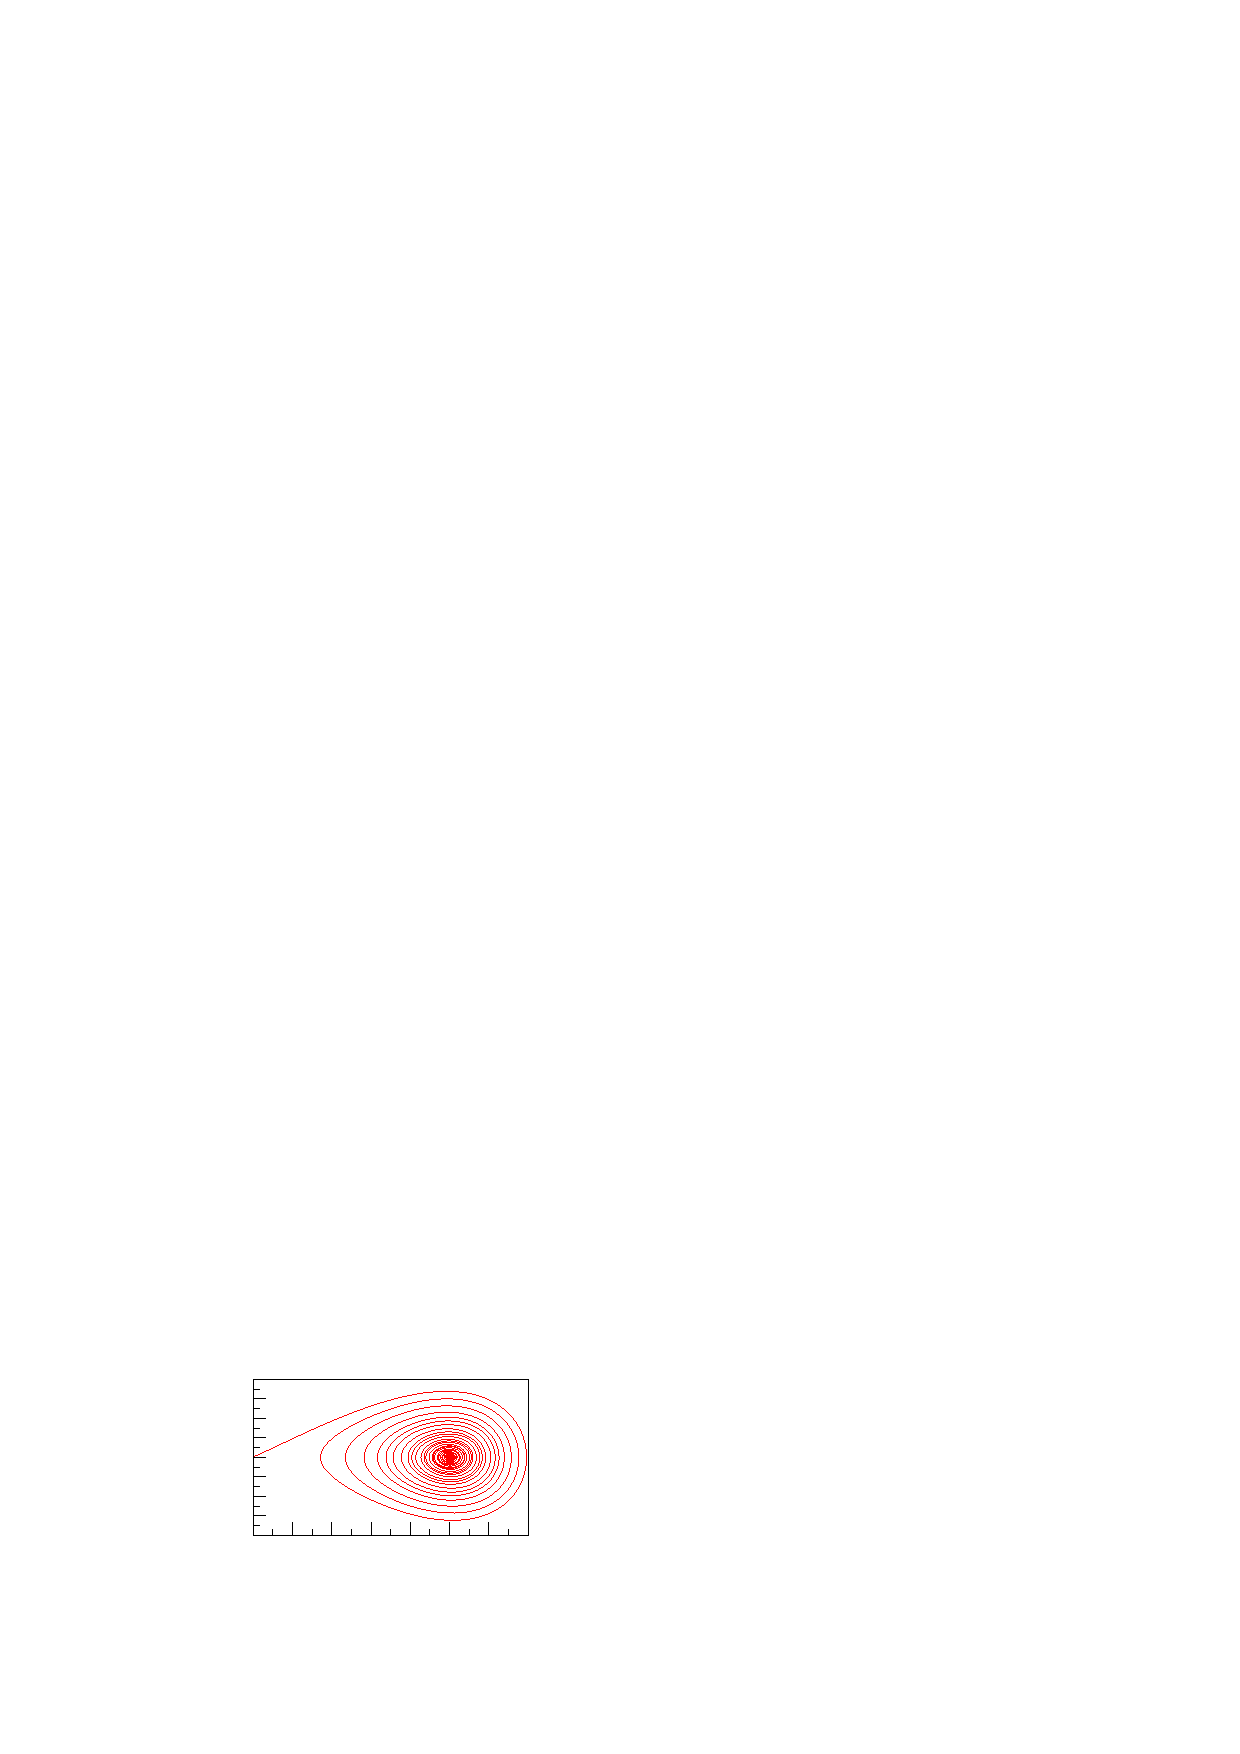
\includegraphics{Images/epslatex/phase1}%
\end{picture}%
\begingroup
\setlength{\unitlength}{0.0200bp}%
\begin{picture}(9900,5940)(0,0)%
\put(2200,1650){\makebox(0,0)[r]{\strut{}-0.8}}%
\put(2200,2117){\makebox(0,0)[r]{\strut{}-0.6}}%
\put(2200,2585){\makebox(0,0)[r]{\strut{}-0.4}}%
\put(2200,3052){\makebox(0,0)[r]{\strut{}-0.2}}%
\put(2200,3520){\makebox(0,0)[r]{\strut{} 0}}%
\put(2200,3988){\makebox(0,0)[r]{\strut{} 0.2}}%
\put(2200,4455){\makebox(0,0)[r]{\strut{} 0.4}}%
\put(2200,4923){\makebox(0,0)[r]{\strut{} 0.6}}%
\put(2200,5390){\makebox(0,0)[r]{\strut{} 0.8}}%
\put(2475,1100){\makebox(0,0){\strut{} 0}}%
\put(3418,1100){\makebox(0,0){\strut{} 0.2}}%
\put(4361,1100){\makebox(0,0){\strut{} 0.4}}%
\put(5304,1100){\makebox(0,0){\strut{} 0.6}}%
\put(6246,1100){\makebox(0,0){\strut{} 0.8}}%
\put(7189,1100){\makebox(0,0){\strut{} 1}}%
\put(8132,1100){\makebox(0,0){\strut{} 1.2}}%
\put(9075,1100){\makebox(0,0){\strut{} 1.4}}%
\put(550,3520){\rotatebox{90}{\makebox(0,0){\strut{}$y$}}}%
\put(5775,275){\makebox(0,0){\strut{}$x$}}%
\end{picture}%
\endgroup
\endinput
 \label{fig:duff_phase_1} }
\subfigure[][]{ %GNUPLOT: LaTeX picture with Postscript
\begin{picture}(0,0)%
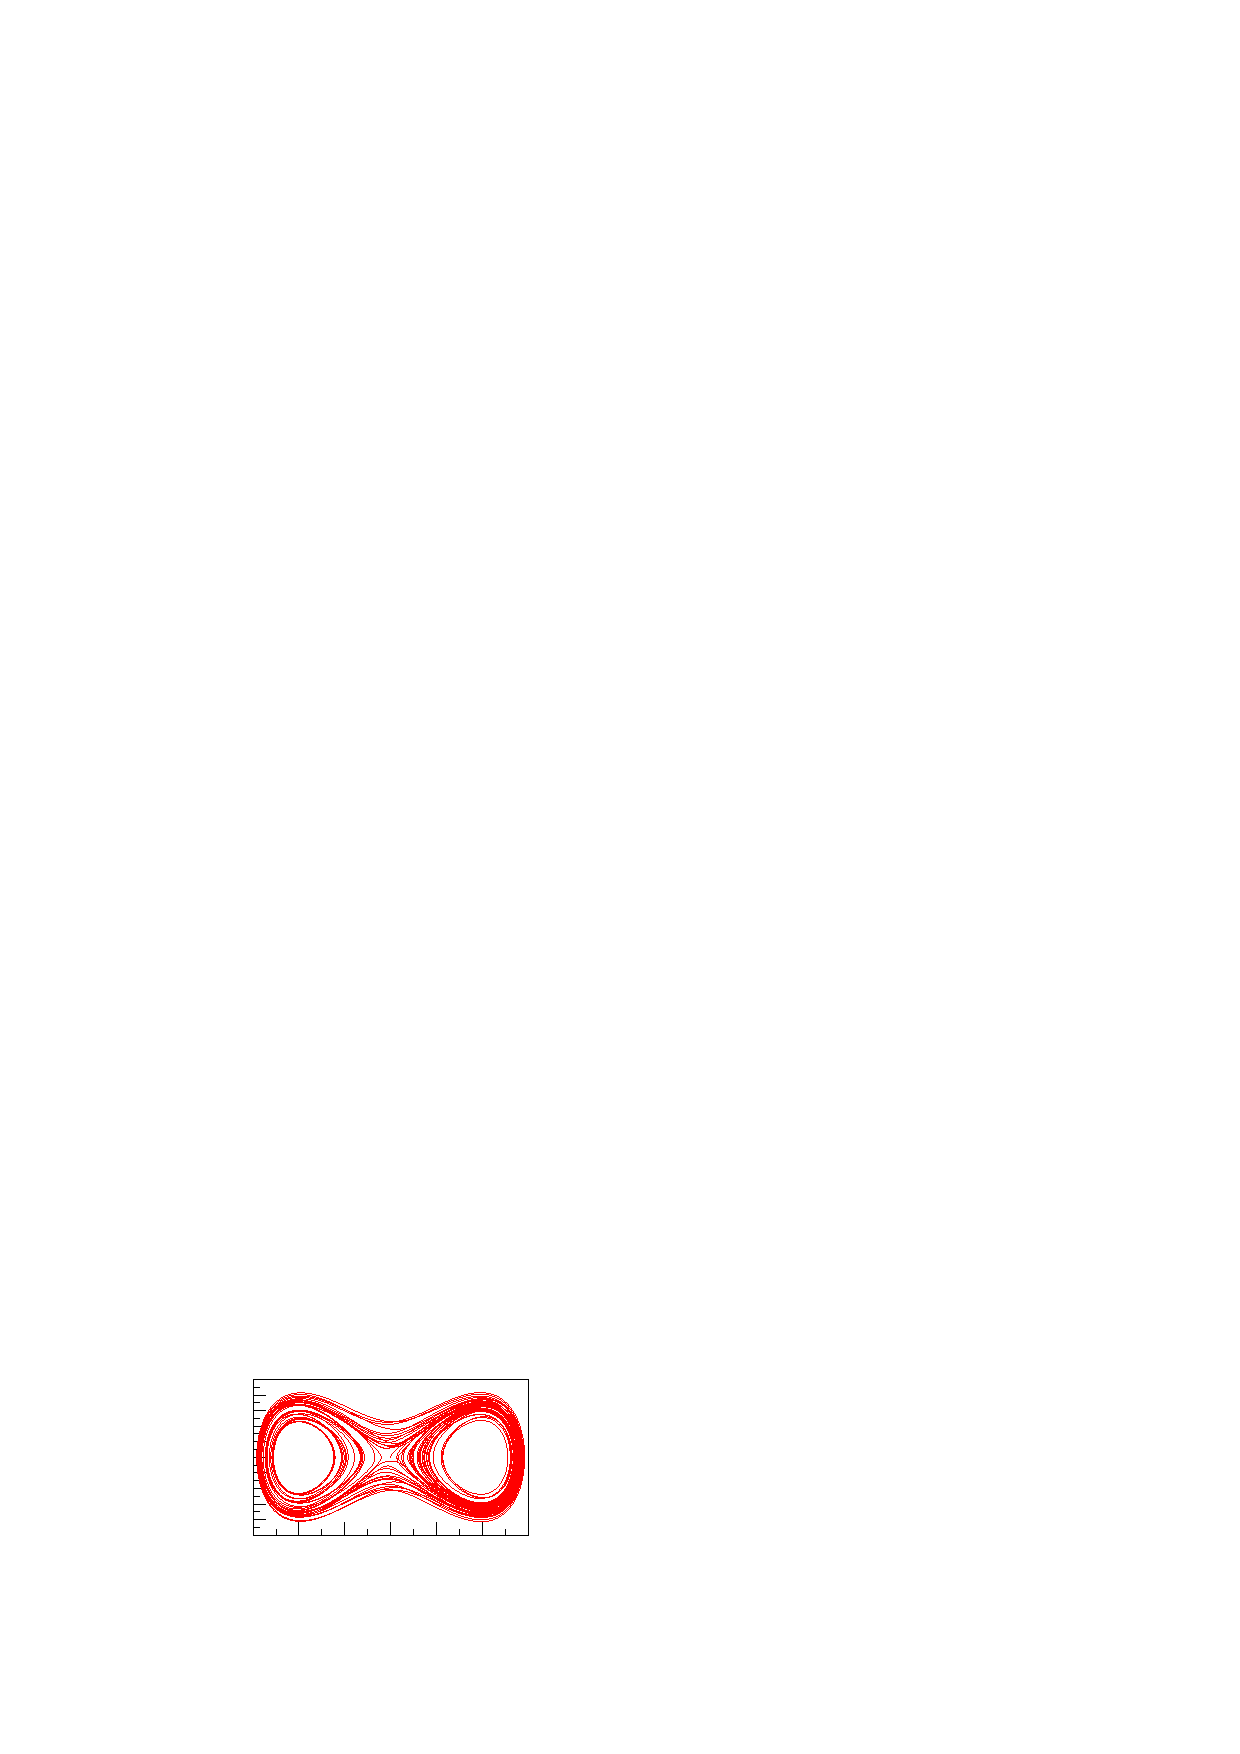
\includegraphics{Images/epslatex/phase2}%
\end{picture}%
\begingroup
\setlength{\unitlength}{0.0200bp}%
\begin{picture}(9900,5940)(0,0)%
\put(2200,1650){\makebox(0,0)[r]{\strut{}-1}}%
\put(2200,2024){\makebox(0,0)[r]{\strut{}-0.8}}%
\put(2200,2398){\makebox(0,0)[r]{\strut{}-0.6}}%
\put(2200,2772){\makebox(0,0)[r]{\strut{}-0.4}}%
\put(2200,3146){\makebox(0,0)[r]{\strut{}-0.2}}%
\put(2200,3520){\makebox(0,0)[r]{\strut{} 0}}%
\put(2200,3894){\makebox(0,0)[r]{\strut{} 0.2}}%
\put(2200,4268){\makebox(0,0)[r]{\strut{} 0.4}}%
\put(2200,4642){\makebox(0,0)[r]{\strut{} 0.6}}%
\put(2200,5016){\makebox(0,0)[r]{\strut{} 0.8}}%
\put(2200,5390){\makebox(0,0)[r]{\strut{} 1}}%
\put(2475,1100){\makebox(0,0){\strut{}-1.5}}%
\put(3575,1100){\makebox(0,0){\strut{}-1}}%
\put(4675,1100){\makebox(0,0){\strut{}-0.5}}%
\put(5775,1100){\makebox(0,0){\strut{} 0}}%
\put(6875,1100){\makebox(0,0){\strut{} 0.5}}%
\put(7975,1100){\makebox(0,0){\strut{} 1}}%
\put(9075,1100){\makebox(0,0){\strut{} 1.5}}%
\put(550,3520){\rotatebox{90}{\makebox(0,0){\strut{}$y$}}}%
\put(5775,275){\makebox(0,0){\strut{}$x$}}%
\end{picture}%
\endgroup
\endinput
 \label{fig:duff_phase_2} }
% \subfigure[][]{ \input{Images/epslatex/poincare1.tex} \label{fig:duff_poincare_1} }
% \subfigure[][]{ \input{Images/epslatex/poincare2.tex} \label{fig:duff_poincare_2} }
\end{center}
\caption[Regular and chaotic Duffing oscillators]{\baselineskip=1.0\normalbaselineskip%
The trajectories and phase diagrams of a regular and irregular Duffing oscillator.}
\label{fig:poincare_duff}
\end{figure} % 
%
\begin{figure}[h!tbp]
\begin{center}
\subfigure[][]{\input{Images/epslatex/u1.tex}\label{fig:u1} }
\subfigure[][]{%GNUPLOT: LaTeX picture with Postscript
\begin{picture}(0,0)%
\includegraphics{Images/epslatex/u2.eps}%
\end{picture}%
\begingroup
\setlength{\unitlength}{0.0200bp}%
\begin{picture}(9900,6480)(0,0)%
\put(2475,1650){\makebox(0,0)[r]{\strut{}-500}}%
\put(2475,2126){\makebox(0,0)[r]{\strut{} 0}}%
\put(2475,2601){\makebox(0,0)[r]{\strut{} 500}}%
\put(2475,3077){\makebox(0,0)[r]{\strut{} 1000}}%
\put(2475,3552){\makebox(0,0)[r]{\strut{} 1500}}%
\put(2475,4028){\makebox(0,0)[r]{\strut{} 2000}}%
\put(2475,4503){\makebox(0,0)[r]{\strut{} 2500}}%
\put(2475,4979){\makebox(0,0)[r]{\strut{} 3000}}%
\put(2475,5454){\makebox(0,0)[r]{\strut{} 3500}}%
\put(2475,5930){\makebox(0,0)[r]{\strut{} 4000}}%
\put(2750,1100){\makebox(0,0){\strut{}-10}}%
\put(3383,1100){\makebox(0,0){\strut{}-8}}%
\put(4015,1100){\makebox(0,0){\strut{}-6}}%
\put(4648,1100){\makebox(0,0){\strut{}-4}}%
\put(5280,1100){\makebox(0,0){\strut{}-2}}%
\put(5913,1100){\makebox(0,0){\strut{} 0}}%
\put(6545,1100){\makebox(0,0){\strut{} 2}}%
\put(7178,1100){\makebox(0,0){\strut{} 4}}%
\put(7810,1100){\makebox(0,0){\strut{} 6}}%
\put(8443,1100){\makebox(0,0){\strut{} 8}}%
\put(9075,1100){\makebox(0,0){\strut{} 10}}%
\put(550,3790){\rotatebox{90}{\makebox(0,0){\strut{}$u_{2}$}}}%
\put(5912,275){\makebox(0,0){\strut{}$t$}}%
\end{picture}%
\endgroup
\endinput
\label{fig:u2} }
\subfigure[][]{%GNUPLOT: LaTeX picture with Postscript
\begin{picture}(0,0)%
\includegraphics{Images/epslatex/x0.eps}%
\end{picture}%
\begingroup
\setlength{\unitlength}{0.0200bp}%
\begin{picture}(9900,6480)(0,0)%
\put(2200,1650){\makebox(0,0)[r]{\strut{} 0}}%
\put(2200,2185){\makebox(0,0)[r]{\strut{} 0.2}}%
\put(2200,2720){\makebox(0,0)[r]{\strut{} 0.4}}%
\put(2200,3255){\makebox(0,0)[r]{\strut{} 0.6}}%
\put(2200,3790){\makebox(0,0)[r]{\strut{} 0.8}}%
\put(2200,4325){\makebox(0,0)[r]{\strut{} 1}}%
\put(2200,4860){\makebox(0,0)[r]{\strut{} 1.2}}%
\put(2200,5395){\makebox(0,0)[r]{\strut{} 1.4}}%
\put(2200,5930){\makebox(0,0)[r]{\strut{} 1.6}}%
\put(2475,1100){\makebox(0,0){\strut{}-10}}%
\put(3135,1100){\makebox(0,0){\strut{}-8}}%
\put(3795,1100){\makebox(0,0){\strut{}-6}}%
\put(4455,1100){\makebox(0,0){\strut{}-4}}%
\put(5115,1100){\makebox(0,0){\strut{}-2}}%
\put(5775,1100){\makebox(0,0){\strut{} 0}}%
\put(6435,1100){\makebox(0,0){\strut{} 2}}%
\put(7095,1100){\makebox(0,0){\strut{} 4}}%
\put(7755,1100){\makebox(0,0){\strut{} 6}}%
\put(8415,1100){\makebox(0,0){\strut{} 8}}%
\put(9075,1100){\makebox(0,0){\strut{} 10}}%
\put(550,3790){\rotatebox{90}{\makebox(0,0){\strut{}$x_{0}$}}}%
\put(5775,275){\makebox(0,0){\strut{}$t$}}%
\end{picture}%
\endgroup
\endinput
\label{fig:x0} }
\subfigure[][]{\input{Images/epslatex/y0.tex}\label{fig:y0} }
\subfigure[][]{\input{Images/epslatex/x1.tex}\label{fig:x1} }
\subfigure[][]{%GNUPLOT: LaTeX picture with Postscript
\begin{picture}(0,0)%
\includegraphics{Images/epslatex/y1}%
\end{picture}%
\begingroup
\setlength{\unitlength}{0.0200bp}%
\begin{picture}(9900,6480)(0,0)%
\put(2200,1650){\makebox(0,0)[r]{\strut{}-1}}%
\put(2200,2506){\makebox(0,0)[r]{\strut{}-0.5}}%
\put(2200,3362){\makebox(0,0)[r]{\strut{} 0}}%
\put(2200,4218){\makebox(0,0)[r]{\strut{} 0.5}}%
\put(2200,5074){\makebox(0,0)[r]{\strut{} 1}}%
\put(2200,5930){\makebox(0,0)[r]{\strut{} 1.5}}%
\put(2475,1100){\makebox(0,0){\strut{}-10}}%
\put(4125,1100){\makebox(0,0){\strut{}-5}}%
\put(5775,1100){\makebox(0,0){\strut{} 0}}%
\put(7425,1100){\makebox(0,0){\strut{} 5}}%
\put(9075,1100){\makebox(0,0){\strut{} 10}}%
\put(550,3790){\rotatebox{90}{\makebox(0,0){\strut{}$y_{1}\left(t,t_{0}^{}\right)$}}}%
\put(5775,275){\makebox(0,0){\strut{}$t$}}%
\end{picture}%
\endgroup
\endinput
\label{fig:y1} }
\caption[First order approximations of modified Duffing oscillator]{\baselineskip=1.0\normalbaselineskip%
Components of the first order perturbations for homoclinic orbits for the modified Duffing oscillator over a suitable range. In these diagrams $\delta=1$, $\omega=1$ and $\gamma=1$. In subfigures~\ref{fig:x1} and~\ref{fig:y1} when $t_{0}=0.1$ is in red, $t_{0}=0.2$ is in dark blue, $t_{0}=0.3$ is in light blue and $t_{0}=0.4$ is in purple. At the points $t=t_0$ the curves are discountinuous.}
\label{fig:new_duffing}
\end{center}
\end{figure} 
%
\chapter{The Cosserat Theory of Elastic Rods} \label{chap:model}
%
In this chapter a system of equations which determine the configurations of a geometrically exact rod under a variety of (generalised) forces is introduced. The rod configurations are determined by the (generalised) strains of the system. The strains are related to the stresses on the rod by a set of constitutive relations, which when hyperelastic allow a variational formulation. A family of balance equations then describe the stresses on the rod. For a thorough exposition of rod theory see~\cite{Antman95}.
%
\section{Kinematic Equations} \label{sec:kinematic}
%
In this section the equations which define a Cosserat rod are introduced. A Cosserat rod is defined by a one-dimensional curve, called the centreline, along which a right-handed orthonormal triad, called the directors, are attached. The centreline describes the position of the rod while the directors describe the orientation of the cross section of the rod. The rod, $\boldsymbol{r}\left(s\right)$, is embedded in the spatial frame as the vector space spanned by the righthanded orthonormal triad of directors $\left\{ \, \boldsymbol{e}_{1}(s), \boldsymbol{e}_{2}(s), \boldsymbol{e}_{3}(s) \, \right\}$. The body frame, also referred to as the director frame, is given by a local rod-centred right-handed orthonormal triad $\left\{ \, \boldsymbol{d}_{1}(s), \boldsymbol{d}_{2}(s), \boldsymbol{d}_{3}(s) \, \right\}$. For clarity vectors in the spatial frame are denoted as $\boldsymbol{p}$ and components of the vector in the director frame form a 3-tuple denoted by the sans serif $\mathsf{p} = \left( \boldsymbol{p}\cdot \boldsymbol{d}_{1}, \boldsymbol{p}\cdot \boldsymbol{d}_{2}, \boldsymbol{p}\cdot \boldsymbol{d}_{3} \right)$. By orthonormality, the directors satisfy
%
\begin{subequations}
\label{eq:orthonormality}
\begin{align}
\boldsymbol{d}_{i}\left( s \right) \cdot \boldsymbol{d}_{j}\left( s \right) & = \delta_{ij}, \quad\quad i = 1,2,3 \quad j=1,2,3 \\
\boldsymbol{d}_{i}\left( s \right) \times \boldsymbol{d}_{j}\left( s \right) & =  \varepsilon_{ijk} \boldsymbol{d}_{k}\left( s \right)
\end{align}
\end{subequations}
%
\begin{figure}[!t] %
\label{fig:rod_diagram} %
\begin{center} %
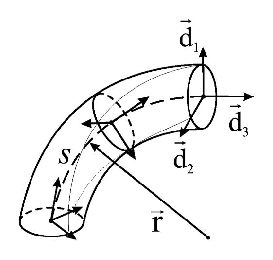
\includegraphics{Images/rod.eps} %
\caption[A Cosserat rod]{\baselineskip=1.0\normalbaselineskip%
Schematic diagram showing the orthornormality of the directors along the arclength.} %
\end{center} %
\end{figure} %
% 
where $\delta_{ij}$ is the Kronecker delta and $\varepsilon_{ijk}$ is the standard Levi-Civita permutation symbol. The orthogonality of the directors shall be exploited throughout the rod models derived. %
%
\par
Let $R$ be an element of the special orthogonal group, $SO\left(3\right)$, i.e. a smooth, left-acting, invertible transformation that converts quantities from the spatial frame into the director frame. Thus
%
\begin{align}
\boldsymbol{d}_{i} & = {R}\boldsymbol{e}_{i} \quad \mbox{for} \quad i = 1,2,3. 
\label{eq:frame}
\end{align}
%
The Lie group $SO\left(3\right)$ consists of the set of all three-by-three skew-symmetric matrices with unit determinant. An element of the corresponding Lie algebra $\mathfrak{so}\left(3\right)$ may be related to an element of $\mathbb{R}^{3}$ through the ``hat map'' isomorphism
%
\begin{equation}
a = \left( a_{1}, a_{2}, a_{3} \right) \in \mathbb{R}^{3} \quad \mbox{and} \quad \hat{a} \in \mathfrak{so}\left(3\right) \quad \mbox{with} \quad \hat{a} \cong 
\left( \begin{array}{ccc}
0 & -a_{3} & a_{2} \\
a_{3} & 0 & -a_{1} \\
-a_{2} & a_{1} & 0 
\end{array} \right) .
\label{eq:isomorphism}
\end{equation}
%
Thus for $\hat{a} \in \mathfrak{so}\left(3\right)$ and $b \in \mathbb{R}^{3}$ then $\hat{a}b = a \times b$.
%
\par
The evolution of the directors along the rod is found by differentiating equation~\eqref{eq:frame} in the spatial frame with respect to the parameter $s$
%
\begin{align}
\boldsymbol{d}^{\prime}_{i} & = {R}^{\prime}_{} \boldsymbol{e}_{i}^{} \nonumber \\
& = {R}^{\prime} {R}^{-T} \boldsymbol{d}_{i} \nonumber \\
& = \hat{\boldsymbol{u}} \boldsymbol{d}_{i} \nonumber \\
& = \boldsymbol{u} \times \boldsymbol{d}_{i} . 
\label{eq:directors}
\end{align}
%
Where $\hat{\boldsymbol{u}}:=R^{\prime}R^{-T}$ and $\boldsymbol{u}$ is defined to be a set of generalised strains. Thus, using the dot product and the orthogonality of the directors, the components of the strain $\boldsymbol{u}$ are expressed as
%
\begin{align}
u_{i}^{} & = \frac{1}{2} \varepsilon_{ijk}^{} \boldsymbol{d}^{\prime}_{j} \cdot \boldsymbol{d}_{k}^{}. \label{eq:curvatures}
\end{align}
%
The second set of strains $\boldsymbol{v}$ are defined as
%
\begin{align}
\boldsymbol{v} & = \boldsymbol{r}^{\prime}. 
\label{eq:centreline}
\end{align}
%
The triples ${\mathsf{u}} = \left( u_{1}, u_{2}, u_{3} \right)$ and ${\mathsf{v}} = \left( v_{1}, v_{2}, v_{3} \right)$ are the generalised strains in the body. Thus the projections onto the director frame $v_{1}=\boldsymbol{v}\cdot\boldsymbol{d}_{1}$ and $v_{2}=\boldsymbol{v}\cdot\boldsymbol{d}_{2}$ are associated with transverse shearing, while $v_{3}=\boldsymbol{v}\cdot\boldsymbol{d}_{3}$ is a measure of extension if positive and compression if negative. Likewise, $u_{1}=\boldsymbol{u}\cdot\boldsymbol{d}_{1}$ and $u_{2}=\boldsymbol{u}\cdot\boldsymbol{d}_{2}$ are associated with torsional bending and $u_{3}=\boldsymbol{u}\cdot\boldsymbol{d}_{3}$ is a measure of the twist in the body. Often the strain $u_{3}$ is referred to as the local twist and is denoted by $\tau=u_{3}$. Since it is natural to assume that rod cannot be compressed to zero length it is assumed
%
\begin{align}
v_{3} & > 0. \nonumber
\end{align}  
%
\par
If a rod is unshearable then
%
\begin{equation}
v_{1} =\boldsymbol{v} \cdot \boldsymbol{d}_{1} = 0 \quad \mbox{and} \quad v_{2} = \boldsymbol{v} \cdot \boldsymbol{d}_{2} = 0.\nonumber
\end{equation} 
%
If a rod is inextensible  
%
\begin{align*}
\left| \boldsymbol{r}^{\prime} \right| & = 1.
\end{align*}
%
Thus, the centreline of an unshearable and inextensible rod is determined by the single condition 
%
\begin{align}
\boldsymbol{r}^{\prime} & = \boldsymbol{d}_{3}
\label{eq:inextensible}
\end{align}
%
and parameter $s$ can now be interpreted as the arc-length of the rod.
%
\section{Constitutive Relationships} \label{sec:constitutive}
%
Having formulated the configurations of a Cosserat rod in terms of the strains $\boldsymbol{u}$ and $\boldsymbol{v}$, in this section the relationship between the stresses and the strains are introduced. 
%
\par
How the strains behave under stress determines the material properties of the rod and the constitutive relations relate the strains to the stresses. If the rod is hyperelastic then there exists a strain density function explicitly dependent on the generalised strains, i.e. $\mathcal{W}\left( \mathsf{u}-\mathsf{u}_{0},\mathsf{v}-\mathsf{v}_{0},s \right)$, such that the components of the force $\mathsf{n}=\left(n_{1},n_{2},n_{3}\right)$ and moment $\mathsf{m}=\left(m_{1},m_{2},m_{3}\right)$ in the body are 
%
\begin{equation}
m_{i} = \frac{\partial \mathcal{W}}{\partial u_{i}} \quad \mbox{and} \quad n_{i} = \frac{\partial \mathcal{W}}{\partial v_{i}},\label{eq:constit}
\end{equation}
%
where $\mathsf{u}_{0}$ and $\mathsf{v}_{0}$ are the strains associated with the unstressed rod. If the rod is uniform then the constitutive relations are the same throughout the rod 
%
\begin{align}
\mathcal{W}\left(\mathsf{u}-\mathsf{u}_{0},\mathsf{v}-\mathsf{v}_{0}\right) & = \mathcal{W}\left( \mathsf{u}-\mathsf{u}_{0},\mathsf{v}-\mathsf{v}_{0},s\right). \label{eq:nondegeneracy_1}
\end{align}
%
A hyperelastic rod will have a convex strain density function, that is the matrix of partial derivatives is positive definite
%
\begin{align}
\left|
\begin{array}{cc}
{\partial \mathsf{m}}\slash{\partial \mathsf{u}} & {\partial \mathsf{m}}\slash{\partial \mathsf{v}} \\
{\partial \mathsf{n}}\slash{\partial \mathsf{u}} & {\partial \mathsf{n}}\slash{\partial \mathsf{v}}
\end{array}
\right| & > 0. \label{eq:nondegeneracy_2}
\end{align}
%
Thus, an increase in the applied bending moment will accompany an increase in the bending strain. The hyperelastic strain function will also be coercive, that is
%
\begin{equation}
\dfrac{ \mathcal{W}\left(\mathsf{u}-\mathsf{u}_{0},\mathsf{v}-\mathsf{v}_{0}\right) }{ \sqrt{ \left|\mathsf{u}\right|^2 + \left|\mathsf{v}\right|^2} } \rightarrow \infty \quad \mbox{as} \quad \left|\mathsf{u}\right|^2 + \left|\mathsf{v}\right|^2 \rightarrow \infty. \label{eq:nondegeneracy_3}
\end{equation}
%
This implies that extremal values of the stresses must accompany extremal values of the strains. Finally, the strain energy density will have a nondegenerate minimum in the unstressed configuration 
%
\begin{align}
0 & = \left. \dfrac{\partial \mathcal{W}}{\partial \mathsf{u}} \right|_{\mathsf{u}=\mathsf{u}_{0},\,\mathsf{v}=\mathsf{v}_{0}} = \left.\dfrac{\partial \mathcal{W}}{\partial \mathsf{v}}\right|_{\mathsf{u}=\mathsf{u}_{0},\,\mathsf{v}=\mathsf{v}_{0}}. \label{eq:nondegeneracy_4}
\end{align}
%
The convexity of the hyperelastic strain-energy density function means that the strains can be inverted (locally) for the stresses, hence the hyperelastic function can be written as $\widetilde{\mathcal{W}}\left(\mathsf{m},\mathsf{n}\right)~\!=~\!\widetilde{\mathcal{W}}\left(\tilde{\mathsf{u}}\left({\mathsf{m}},{\mathsf{n}}\right),\tilde{\mathsf{v}}\left({\mathsf{m}},{\mathsf{n}}\right)\right)$. This assumption is crucial in that it allows the hyperelastic function to be related to the Hamiltonion via the Legendre transform. %
%
\par
An important property of many rod is isotropy. Assuming the material is transversally isotropic requires 
%
\begin{equation}
\tilde{\mathsf{u}}\left( Q \mathsf{m}, Q\mathsf{n}, s \right) = Q \tilde{\mathsf{u}}\left(\mathsf{m},\mathsf{n},s\right) \quad \mbox{and} \quad \tilde{\mathsf{v}}\left( Q \mathsf{m}, Q\mathsf{n}, s \right) = Q \tilde{\mathsf{v}}\left(\mathsf{m},\mathsf{n},s\right), \label{eq:isotropic}
\end{equation}
%
where $Q$ is a constant orthogonal matrix of the form 
%
\begin{align}
Q & = \left( 
\begin{array}{ccc}
Q_{11} & Q_{12} & 0 \\
Q_{21} & Q_{22} & 0 \\
0 & 0 & 1 
\end{array}
\right). \nonumber
\end{align}
%
It can be shown~\cite{Antman81} using Cauchy's Representation Theorem, that for nonlinear isotropic constitutive relationships the strain density function takes the arguments
%
\begin{align}
\widetilde{\mathcal{W}} & = \widetilde{\mathcal{W}}\left( m_{1}^{2} + m_{2}^{2}, m_{3}^{}, n_{1}^{2}+n_{2}^{2}, n_{3}^{}, m_{1}^{}n_{1}^{}+m_{2}^{}n_{2}^{}, m_{1}^{}n_{2}^{}-m_{2}^{}n_{1}^{}\right) .
\label{eq:constitutive_constraints}
\end{align}
%
\par
For an inextensible, unshearable rod the strain-density function for an initially straight and untwisted rod is a function of the strains ${\mathsf{u}}$ only, that is, $\mathsf{u}_{0} = \left(0,0,0\right)$ and $\mathsf{v} = \mathsf{v}_{0} = \left(0,0,1\right)$. In fact, for a rod under end tension and moment, nonlinear constitutive laws make little difference either in the underlying structure or the effective localised buckling modes for a rod under end tension and moment~\cite{Antman75,Champneys96b}. However, in order to separate nonlinear geometric effects from those caused by material nonlinearity, linear constitutive laws will be taken throughout. For simplicity, quadratic form, linear constitutive relationships, satisfying Hooke's law are chosen. The strain density function is given by 
%
\begin{align}
\mathcal{W} \left( {\mathsf{u}}, {\mathsf{v}} \right) & = \frac{1}{2}B_{1}\left(u_{1}+u_{0}\right)^{2} + \frac{1}{2}B_{2}u_{2}^{2} + \frac{1}{2} C u_{3}^{2} + \frac{1}{2} H v_{1}^{2} + \frac{1}{2} J {v_{2}^{2}} + \frac{1}{2} K v_{3}^{2}.
\label{eq:hyperelastic}
\end{align}
%
The constants $B_{1}=EI_{1}$, $B_{2}=EI_{2}$ and $C=GI_{3}$, where $I_{1}$ and $I_{2}$ are the principal moments of inertia about the $\boldsymbol{d}_{1}$ and $\boldsymbol{d}_{2}$ axes respectively, $I_{3}$ is the moment of inertia about the $\boldsymbol{d}_{3}$ axis, $E$ is Young's modulus and 
%
\begin{align}
G & = \frac{E}{2 \left(1+\nu\right)}\nonumber
\end{align} 
%
is the shear modulus, where $\nu$ is Poisson's ratio. The constants $H$ and $J$ are transverse shear stiffnesses and $K$ is the axial stiffness. The constant $u_{0}$ is a degree of initial curvature. It follows that $m_{1}$ and $m_{2}$ are associated with bending about the principal axes, $m_{3}$ with twist, $n_{1}$ and $n_{2}$ with shearing forces and $n_{3}$ with tension if positive, compression if negative. In the case of isotropy then $B_{1}=B_{2}$ and $H=J$.
%
\par
Having previously outlined how the rod configurations are determined by the strains and the relationships between strain and applied stress, in order to close the system it is now necessary to describe the structure of the applied stresses. 
%
\section{Equilibrium Equations} \label{sec:equilibrium}
%
In this section the static equilibrium balance equations are introduced. This is the final piece of information needed in order to construct the rod configuration. It shall be assumed that all forces and moments are suitable averages over the rod's cross section acting at the centreline of the rod. 
%
\subsection{Force-Free Rod} \label{subsec:twisted_equation}
%
In the spatial frame the equilibrium equation for a rod under constant end torque is
%
\begin{align}
\boldsymbol{m}^{\prime} & = \boldsymbol{0}.
\label{eq:fixed_frame}
\end{align}
% 
In the director frame the equation can be written as a non-canonical Hamiltonian system
%
\begin{align}
\mathsf{m}^{\prime} & = \mathcal{J}\left(\mathsf{m}\right) \nabla \mathcal{H}\left(\mathsf{m}\right),
\label{eq:noncan}
\end{align}
%
where the skew-symmetric structure matrix $\mathcal{J}= \mathcal{J}\left(\mathsf{m}\right)$ is given by
%
\begin{align}
\mathcal{J} & = -\mathcal{J}^{T} =
\left( 
\begin{array}{ccc}
0 & -m_{3} & m_{2} \\
m_{3} & 0 & -m_{1} \\
-m_{2} & m_{1} & 0 
\end{array} 
\right)
\label{eq:twist_structure}
\end{align}
%
and the Hamiltonian is
%
\begin{align}
\mathcal{H} & = \frac{1}{2} \mathsf{m} \cdot \mathsf{u}\left(\mathsf{m}\right) ,
\label{eq:twisted_hamiltonian}
\end{align}
%
with the strains as given in~\eqref{eq:constit}. For any two functions, $f$ and $g$ of $\mathsf{m}$, the Lie-Poisson bracket on the dual of the Lie algebra $\mathfrak{so}\left(3\right)$, corresponding to the structure matrix~\eqref{eq:twist_structure}, is given by
%
\begin{align}
\left\{ f , g \right\}_{\left(\mathsf{m}\right)} & = - \underbrace{ \mathsf{m} \cdot \left( \nabla_{\mathsf{m}}f \times \nabla_{\mathsf{m}} g \right) }_{\mbox{twist}}, 
\label{eq:twisted_bracket}
\end{align} 
%
where the Lie bracket is given by the direct sum of elements 
%
\begin{align}
\left[ {\xi}, {\eta} \right] & = \xi \times \eta \label{eq:direct_sum}
\end{align}
%
and the inner product is the dot product. Thus the governing equation~\eqref{eq:noncan} can be written as
%
\begin{align}
\mathsf{m}^{\prime} & = \left\{ \mathsf{m}, \mathcal{H}\right\}_{(\mathsf{m})} = \mathsf{m} \times \mathsf{u} . 
\label{eq:twisted}
\end{align}
%
\par
Note that when the constitutive relations are linear the Hamiltonian is quadratic and thus positive definite, hence the configurations are geodesic.
% 
\par
The null-space of the structure matrix~\eqref{eq:twist_structure} is one-dimensional and is spanned by the gradient of the Casimir
%
\begin{align}
\nabla C_{1} & = \frac{1}{2} \left( m_{1}, m_{2}, m_{3} \right)^{T} \nonumber
\end{align}
%
and hence
%
\begin{align}
C_{1} & = \mathsf{m} \cdot \mathsf{m}
\label{eq:twisted_casimir}
\end{align}
%
is a Casimir. The Casimir simply describes the fact that the magnitude of the total moment is constant along the rod. Since $\mathcal{H}$ is an integral, it follows from the Arnol'd-Liouville theorem~\ref{def:integrability} that~\eqref{eq:twisted} is completely integrable. In fact, the force-free rod is globally superintegrable~\cite{Fasso96,Fasso05,Hanssmann05}.
%
\par
Having introduced the Lie-Poisson bracket for the equilibrium equations, the strains can be computed from the constitutive relations and the centreline of the rod can then be recovered. In most practical applications however the boundary conditions will feature conditions on the orientation of the rod. The evolution of the fixed vectors in the director frame can be incorporated into the Lie-Poisson framework as a semidirect extension to the existing bracket. Thus, the evolution of centreline can be recovered from the field variables. The complete set of equations are 
%
\begin{align}
\left\{ f, g \right\}_{\left(\mathsf{m},\mathsf{e}_{1},\mathsf{e}_{2},\mathsf{e}_{3}\right)} & = \mathsf{m} \cdot \left( \nabla_{\mathsf{m}}f \times \nabla_{\mathsf{m}} g \right) + \mathsf{e}_{1} \cdot \left( \nabla_{\mathsf{m}}f \times \nabla_{\mathsf{e}_{1}} g + \nabla_{\mathsf{e}_{1}}f \times \nabla_{\mathsf{m}} g\right) \nonumber \\
& \hspace{2.0cm} + \mathsf{e}_{2} \cdot \left( \nabla_{\mathsf{m}}f \times \nabla_{\mathsf{e}_{2}} g + \nabla_{\mathsf{e}_{2}}f \times \nabla_{\mathsf{m}} g\right) \nonumber \\
& \hspace{2.5cm} + \mathsf{e}_{3} \cdot \left( \nabla_{\mathsf{m}}f \times \nabla_{\mathsf{e}_{3}} g + \nabla_{\mathsf{e}_{3}}f \times \nabla_{\mathsf{m}} g\right) \nonumber 
\nonumber
\end{align}
%
The extended Lie algebra is now given by $\mathfrak{so}\left(3,3\right) = \mathfrak{so}\left(3\right) \oplus_{s}\left( \mathbb{R}^{3} \times \mathbb{R}^{3} \times \mathbb{R}^{3}\right)$ but as the Hamiltonian is indepedent of the spatial frame the extensions to the bracket do not effect the configurations of the rod.
%  
\subsection{Kirchhoff Rod} \label{subsec:kirchhoff_equation}
%
The equilibrium equations for a rod under end tension and moment are given by
%
\begin{equation}
\boldsymbol{m}^{\prime} + \boldsymbol{r}^{\prime} \times \boldsymbol{n}=\boldsymbol{0} \quad \mbox{and} \quad \boldsymbol{n}^{\prime} = \boldsymbol{0}. 
\label{eq:kirchhoff_external}
\end{equation}
%
In the director frame the equations can be written in Hamiltonian form as
%
\begin{align}
\left( 
\begin{array}{c}
\mathsf{m} \\
\mathsf{n} 
\end{array}
\right)^{\prime} & = 
\mathcal{J}\left(\mathsf{m}, \mathsf{n}\right) \nabla \mathcal{H}\left( \mathsf{m}, \mathsf{n}\right),
\end{align}
%
where the structure matrix $\mathcal{J} = \mathcal{J}\left(\mathsf{m},\mathsf{n}\right)$ is given by
%
\begin{align}
\mathcal{J} & = -\mathcal{J}^{T} = 
\left( \begin{array}{cc} 
\hat{\mathsf{m}} & \hat{\mathsf{n}} \\
\hat{\mathsf{n}} & 0 
\end{array}
\right)
\label{eq:kirchhoff_structure}
\end{align}
%
and the Hamiltonian is now
%
\begin{align}
\mathcal{H} & = \frac{1}{2}\mathsf{m}\cdot\mathsf{u}\left(\mathsf{m},\mathsf{n}\right) +  \frac{1}{2}\mathsf{n}\cdot\mathsf{v}\left(\mathsf{m},\mathsf{n}\right). 
\label{eq:kirchhoff_hamiltonian}
\end{align}
% 
Thus the additional term can be considered to be the kinetic energy-density due to the end force.  The governing equations are
%
\begin{subequations}
\label{eq:kirchhoff}
\begin{align}
\mathsf{m}^{\prime} & = \left\{\mathsf{m}, \mathcal{H} \right\}_{(\mathsf{m},\mathsf{n})} = \mathsf{m} \times \mathsf{u} + \mathsf{n} \times \mathsf{v}, \label{eq:kirchhoff_moment} \\
\mathsf{n}^{\prime} & = \left\{\mathsf{n}, \mathcal{H} \right\}_{(\mathsf{m},\mathsf{n})} = \mathsf{n} \times \mathsf{u}  \label{eq:kirchhoff_force}.
\end{align}
\end{subequations}
%
which are the Lie-Poisson equations on the Cartesian pairing $\left( \mathsf{m}, \mathsf{n} \right)$ given by the bracket
%
\begin{align}
\left\{ f , g \right\}_{\left({\mathsf{m}},{\mathsf{n}}\right)} & = - \mathsf{m} \cdot \left( \nabla_{\mathsf{m}}f \times \nabla_{\mathsf{m}} g \right) - \underbrace{ \mathsf{n} \cdot \left( \nabla_{\mathsf{m}}f \times \nabla_{\mathsf{n}} g + \nabla_{\mathsf{n}}f \times \nabla_{\mathsf{m}} g\right) }_{\mbox{force}}.
\label{eq:kirchhoff_bracket}
\end{align}
%
An extra semidirect term, corresponding to the effect of the end force has been added when compared to the previous Lie-Poisson bracket~\eqref{eq:twisted_bracket}. Again the inner product is dot product but the Lie algebra now has the bracket 
%
\begin{align}
\left[ \left( \xi, u \right), \left( \eta, v\right) \right] & = \left( \xi\times\eta, \xi \times v - \eta \times u \right) .
\end{align}
%
Where $\left(\xi,u\right) \in \mathfrak{g}$. The Lie algebra is then given by $\mathfrak{g} = \mathfrak{so}\left(3,1\right) = \mathfrak{so}\left(3\right)\oplus_{s}\mathbb{R}^{3}$ and the moment $\mathsf{m}$ spans $\mathfrak{so}\left(3\right)$ and the force $\mathsf{n}$ spans $\mathbb{R}^{3}$. The associated Lie group now corresponds to the group of rotations and translations in~$\mathbb{R}^{3}$. As shall be shown in chapter~\ref{chap:reduction} knowledge of the underlying group is extremely helpful when reducing the system. 
%
\par
The additional term in the Hamiltonian, due to the end force, breaks the full $SO\left(3\right)$ symmetry. The equations~\eqref{eq:kirchhoff} are those for the motion of a heavy top when the rod is unshearable and inextensible.
% 
\par
The null-space of the structure matrix is two-dimensional and spanned by
%
\begin{equation}
\nabla C_{1} = \left(\begin{array}{c} \mathsf{n} \\ \mathsf{m} \end{array} \right) \quad \mbox{and} \quad \nabla C_{2} = \frac{1}{2} \left(\begin{array}{c} \mathsf{0} \\ \mathsf{n} \end{array} \right). \nonumber
\end{equation}
%
Hence the Casimirs are 
%
\begin{subequations}
\label{eq:kirchoff_casimirs}
\begin{align}
C_{1} & = \mathsf{n} \cdot \mathsf{m} \label{eq:kirchhoff_casimir1}, \\
C_{2} & = \mathsf{n} \cdot \mathsf{n} \label{eq:kirchhoff_casimir2}.\
\end{align} 
\end{subequations}
%
The Casimir~\eqref{eq:kirchhoff_casimir1} describes the conservation of the moment about the force vector, while~\eqref{eq:kirchhoff_casimir2} describes the conservation of the magnitude of force in the rod. 
%
\par
In addition to the Hamiltonian and the two Casimirs, a single first integral is required if the system is to be completely integrable.  There are two cases, both well-documented:
%
\begin{description}
\item[The Lagrange case] has an integral given by
\begin{align}
I_{1} &= \mathsf{m} \cdot \mathsf{d}_3 \quad \mbox{if} \quad B_{1} = B_{2} = B. \label{eq:lagrange}
\end{align}
Thus, if the two bending stiffnesses are equal then the (local) twist $m_3$ is a conserved quantity. For the Kirchhoff equation if the rod satisfies~\eqref{eq:isotropic} then the Lagrange integral holds for arbitrary nonlinear constitutive relationships. 
\item[The Kovalevskaya case] has an integral given by
\begin{align}
I_{1} & = \left( B_{1}^{2}m_{1}^{2} - C^{2} m_{3}^{2} + n_{3} \right)^{2} 
+ \left( 2 B_{1}^{} C m_{1}m_{3} - n_{1} \right)^{2} \quad \mbox{if} \quad B_{1} = C = 2B_{2}.
\label{eq:kov}
\end{align}
% 
Kovalevskaya found this integral by looking for the absence of certain types of singularities in complex time. Unlike the Lagrange integral the integral does not seem to have a clear physical interpretation.\footnote{Kovalevskaya won the Bordin Prize given by the Paris Academy of Sciences in 1886 and was considered such a achievement that the prize money was doubled.}
%
\par  
The condition on the bending stiffnesses renders the Kovalevskaya rod somewhat unphysical since it corresponds to a negative Poisson ratio. However, novel materials with negative effective Poisson ratio are now known. For instance, experimental measurements of bending and torsional stiffnesses of DNA molecules have led to the generally accepted range $0.7<K/K_3<1.5$~\cite{Schlick95}. It is unknown how nonlinear constitutive relations or properties such as shear and extensibility effect the Kovalevskaya integral.
\end{description}
%
There is another case which is not completely integrable on the entire phase space but is completely integrable on a single symplectic leaf.
%
\begin{description}
\item[The Chaplygin-Goryachev case] requires that the initial conditions must satisfy
\begin{align}
\mathsf{m} \cdot \mathsf{n} & = \mathsf{0} \nonumber
\end{align}
then the integral
\begin{align}
I_{1} = B_{2}^{} m_{2} \left( B_{1}^{2} m_{1}^{2} + B_{2}^{2}m_{2}^{2} \right) - C m_{3} n_{2} \quad \mbox{if} \quad B_{1} = 4 B_{2} = C \label{eq:chaplygin}
\end{align}
renders the system integrable. Similarly to the Kovalevskaya integral, this case relies on linear stress-strain relationships and it is unknown whether a corresponding integral exist for nonlinear constitutive relations. The only natural interpretation of the condition on the Casimir is to not apply end moment and then the Chaplygin-Goryachev case can be considered an anisotropic case of the elastica.  
\end{description}
%
It is simple to show that all the integrals~\eqref{eq:kirchoff_casimirs},~\eqref{eq:kirchhoff_hamiltonian} and either~\eqref{eq:lagrange},~\eqref{eq:kov}, or~\eqref{eq:chaplygin} are in involution with respect to the bracket~\eqref{eq:kirchhoff_bracket} and that generically integrable configurations exist on three-tori.
%
\subsection{An Elastic Conducting Rod in a Uniform Magnetic Field}\label{subsec:magnetic_equation}
%
Now consider a rod placed in a uniform magnetic field $\bar{\boldsymbol{B}}$. The rod carries a uniform current $\boldsymbol{I}=I\boldsymbol{r}^{\prime}$ of strength $I$ along the centreline, assuming the rod to be sufficiently slender for eddy currents within the cross section to be ignorable. The rod then experiences a Lorentz body force 
% 
\begin{align}
\boldsymbol{n}^{\prime} + \boldsymbol{F}_{L} & = \boldsymbol{0} \quad \mbox{where} \quad \boldsymbol{F}_L=\boldsymbol{I}\times\bar{\boldsymbol{B}} = I\boldsymbol{r}^{\prime}\times\bar{\boldsymbol{B}} = I\boldsymbol{v}\times\bar{\boldsymbol{B}}. 
\end{align}
% 
Let $\boldsymbol{B}=I\bar{\boldsymbol{B}}$ and let the magnetic field be aligned along the fixed axis $\boldsymbol{e}_{3}$ so that the equilibrium equations take the form
%
\begin{align}
\boldsymbol{m}^{\prime} + \boldsymbol{r}^{\prime} \times \boldsymbol{n}=\boldsymbol{0},  \quad  \boldsymbol{n}^{\prime} +  \boldsymbol{r}^{\prime} \times \boldsymbol{B}=\boldsymbol{0} \quad \mbox{and} \quad \boldsymbol{B}^{\prime} = \boldsymbol{0}.
\label{eq:magnetic}
\end{align}
%
It is necessary to assume that the current in the rod is moderate so that the effect of the magnetic field generated by the current is negligible compared to the external magnetic field.  
%
\par
In the director frame the governing equation is a non-canonical Hamiltonian system of the form
%
\begin{align}
\left(
\begin{array}{c}
\mathsf{m} \\
\mathsf{n} \\
\mathsf{B}
\end{array}
\right)^{\prime} & =
\mathcal{J} \left({\mathsf{m}},{\mathsf{n}},\mathsf{B}\right) \nabla \mathcal{H}\left({\mathsf{m}},{\mathsf{n}} \right),
\label{eq:noncanonical_structure}
\end{align}
%
where the structure matrix $\mathcal{J}=\mathcal{J} \left( \mathsf{m}, \mathsf{n}, \mathsf{B} \right)$ is given by
%
\begin{align}
\mathcal{J} = -\mathcal{J}^{T} & = \left( 
\begin{array}{ccc}
\hat{\mathsf{m}} & \hat{\mathsf{n}} & \hat{\mathsf{B}} \\
\hat{\mathsf{n}} & \hat{\mathsf{B}} & \mathsf{0} \\
\hat{\mathsf{B}} & \mathsf{0} & {\mathsf{0}}  
\end{array}
\right)
\label{eq:magnetic_structure}
\end{align}
%
and the Hamiltonian, once again, is 
%
\begin{align}
\mathcal{H} & = \frac{1}{2} \mathsf{m} \cdot \mathsf{u} + \mathsf{n}\cdot\mathsf{v}. \label{eq:magnetic_ham}
\end{align}
%
Note that the Hamiltonian is a function of $\mathsf{m}$ and $\mathsf{n}$ only, but the gradient is taken with respect to the three field variables. The Hamiltonian is the same as for the Kirchhoff rod: the effect of the magnetic field is only present in the structure matrix.  The governing equations can be written as
%
\begin{subequations}
\label{eq:magnetic_equations}
\begin{align}
\mathsf{m}^{\prime} & = \left\{\mathsf{m}, \mathcal{H} \right\}_{\left({\mathsf{m}},{\mathsf{n}}, {\mathsf{B}} \right)} = \mathsf{m}\times\mathsf{u} + \mathsf{n}\times\mathsf{v}, \label{eq:magnetic_moment} \\
\mathsf{n}^{\prime} & = \left\{\mathsf{n}, \mathcal{H} \right\}_{\left({\mathsf{m}},{\mathsf{n}}, {\mathsf{B}} \right)} = \mathsf{n}\times\mathsf{u} + \mathsf{B}\times\mathsf{v}, \label{eq:magnetic_force} \\
\mathsf{B}^{\prime} & = \left\{\mathsf{B}, \mathcal{H} \right\}_{\left({\mathsf{m}},{\mathsf{n}}, {\mathsf{B}} \right)} = \mathsf{B}\times\mathsf{u}, \label{eq:magnetic_vector}
\end{align}
\end{subequations}
%
where the Lie-Poisson bracket on $\left( \mathsf{m}, \mathsf{n}, \mathsf{B} \right)$ given by
%
\begin{align}
\left\{ f,g \right\}_{\left({\mathsf{m}},{\mathsf{n}}, {\mathsf{B}} \right)} & =
- {\mathsf{m}}\cdot\left(\nabla_{{\mathsf{m}}}f \times \nabla_{{\mathsf{m}}}g \right) 
- {\mathsf{n}}\cdot\left(\nabla_{{\mathsf{m}}}f \times \nabla_{{\mathsf{n}}}g + \nabla_{{\mathsf{n}}}f \times \nabla_{{\mathsf{m}}}g\right) \nonumber \\
& \hspace{1.25cm} - \underbrace{{\mathsf{B}} \cdot \left(\nabla_{\mathsf{m}}f \times \nabla_{\mathsf{B}}g +
\nabla_{\mathsf{B}}f \times \nabla_{{\mathsf{m}}}g \right)}_{\mbox{evolution of field}}
- \underbrace{\mathsf{B} \cdot \left( \nabla_{\mathsf{n}}f \times \nabla_{\mathsf{n}}g \right)}_{\mbox{effect of field}},
\label{eq:magnetic_bracket}
\end{align}
%
has been extended from the previous bracket by the addition of two more terms. The first term, a semidirect extension, describes the evolution of the magnetic field in the director frame and does not affect the force and moment balance since the Hamiltonian is independent of $\mathsf{B}$. The second term, called a Liebniz extension~\cite{Thiffeault00}, contains the Lorentz force. This term makes the bracket extension non-semidirect.  %
%
\begin{rem}
In the language of Lie algebra cohomology the bracket is extended by a semidirect and a Liebniz extensions. Cohomology studies the connections between the topology of the Lie group and the algebraic structure of the associated Lie algebra. Cohomology gives a class of linear transformations that preserve the structure of the normal forms of the bracket extensions. The parts of the extensions that are removed by such transformations are called coboundaries, those that remain are called cocycles. Cocycles are bilinear skew-symmetric functions on the Lie algebra which satisfy Jacobi's identity~\cite[pg.~372]{Arnold89}. The Liebniz extension is a cocycle and as the Hamiltonian is independent of the spatial frame, the semidirect extension is a coboundary. %
\end{rem}
% 
\par
The bracket which generates the Lie algebra is given by
%
\begin{align}
\left[ \left( \xi, u, w \right), \left( \eta, v, x \right) \right] & = \left( \xi\times\eta, \, \xi \times v - \eta \times u, \, \xi \times w - \eta \times x -  u \times v \right).\label{eq:bracket3}
\end{align}
%
Even though the nontrivial extension is of the simplest possible form~\cite{Thiffeault00} it leads to highly nontrivial generalisations of the symmetry groups. The Lie algebra includes $\mathfrak{so}\left(3\right)$ and $\mathbb{R}^{3}$ as proper subalgebras but is not purely composed of the semi-direct sum of the subalgebras. %
% 
\par
There are three Casimirs, given by
%
\begin{subequations}
\label{eq:magnetic_casimirs}
\begin{align}
C_{1} & = \frac{1}{2}\mathsf{n} \cdot \mathsf{n} + \mathsf{m} \cdot \mathsf{B}, \label{eq:magnetic_casimirs1} \\
C_{2} & = \mathsf{B} \cdot \mathsf{n}, \label{eq:magnetic_casimirs2} \\
C_{3} & = \mathsf{B} \cdot \mathsf{B}. \label{eq:magnetic_casimirs3}
\end{align} 
\end{subequations}
%
The magnitude of the magnetic force is conserved, thus~\eqref{eq:magnetic_casimirs3}. The magnitude of force is no longer conserved, but as a result of rotational symmetry the force component in the direction of the magnetic field is conserved resulting in~\eqref{eq:magnetic_casimirs2}. Casimir~\eqref{eq:magnetic_casimirs1} however does not seem to have a physical interpretation; it states that half the magnitude of the force in the body plus the moment about the direction of the magnetic field is a conserved quantity. %
%
\par
In the linearly elastic~\eqref{eq:hyperelastic}, unshearable, inextensible and isotropic case, that is $J=H=K=0$ and $B=B_1=B_2$, then two integrals emerge
%
\begin{subequations}
\label{eq:magnetic_integrals}
\begin{align}
I_{1} & = \mathsf{m}\cdot\mathsf{d}_3, \label{eq:magnetic_lagrange} \\
I_{2} & = \mathsf{n}\cdot\mathsf{m} + B \mathsf{B} \cdot \mathsf{d}_{3}. \label{eq:int2}
\end{align}
\end{subequations}
%
As in the Lagrange case the first of these integrals expresses the conservation of twist in the rod. The second integral, like the Kovalevskaya integral, does not seem to have a physical interpretation. The Lagrange integrability condition $B_1=B_2$ is unaltered by the magnetic field, but now there are additional requirements on constitutive relations in the form of linear elasticity, inextensibilty and shearability. Numerical evidence presented in~\cite{Thiffeault01} in the form of chaotic orbits suggests that the linearly elastic, inextensible, unshearable the magnetic rod with $B_1=C=2B_{2}$ is not integrable. Of course, a perturbed condition on the stiffnesses may exist for which the system is integrable. %
%
\par
It is a straightforward task to check that all the integrals~\eqref{eq:magnetic_ham},~\eqref{eq:magnetic_lagrange} and~\eqref{eq:int2} are independent and in involution with respect to the Lie-Poisson bracket~\eqref{eq:magnetic_bracket}. Hence in the isotropic case the system is completely integrable in the sense of Liouville and configurations lie on five-tori defined by two Casimirs, two integrals and the Hamiltonian. %
% 
\par
Note that due to the complexities of the Lie algebra, the Lie group which generates the Lie algebra is not known. That the underlying Lie group is not known means that a suitable parameterisation can not be constructed which gives a complete representation of the symmetries and hence integrals. Thus, presently, the system can not be reduced to a single degree of freedom canonical Hamiltonian system. %
%
\subsection{An Elastic Conducting Rod in a Nonuniform Magnetic Field} \label{subsec:twisted_field}
%
By inspection of the structure matrices~\eqref{eq:twist_structure},~\eqref{eq:kirchhoff_structure} and~\eqref{eq:magnetic_structure} it is natural to consider the system
%
\begin{align}
\boldsymbol{m}^{\prime} + \boldsymbol{r}^{\prime}\times\boldsymbol{n} = \boldsymbol{0}, \quad \boldsymbol{n}^{\prime} + \boldsymbol{r}^{\prime}\times\boldsymbol{B}=\boldsymbol{0}, \quad \boldsymbol{B}^{\prime} + \boldsymbol{r}^{\prime}\times\boldsymbol{D}=\boldsymbol{0} \quad \mbox{and} \quad \boldsymbol{D}^{\prime} = \boldsymbol{0}.
\label{eq:nonuniform_vec}
\end{align}
%
The equation for $\boldsymbol{B}$ can be integrated to give $B_x=y$, $B_y=-x$, $B_z=0$, where $x,y,z$ and $B_x,B_y,B_z$ are components of $\boldsymbol{r}$ and $\boldsymbol{B}$ relative to the fixed frame $\{\boldsymbol{e}_1,\boldsymbol{e}_2,\boldsymbol{e}_3\}$, and $\boldsymbol{e}_3$ is choosen to be in the direction of $\boldsymbol{D}$. Thus~\eqref{eq:nonuniform_vec} can be thought of as describing a rod in a linearly-varying magnetic field generated by a uniform `hypermagnetic' field $\boldsymbol{D}$. %
%
\par
In the director frame the equations take the Hamiltonian form
%
\begin{align}
\left( \begin{array}{cccc} 
\mathsf{m} \\
\mathsf{n} \\
\mathsf{B} \\
\mathsf{D}
\end{array} \right)^{\prime} & = \mathcal{J}\left( \mathsf{m}, \mathsf{n}, \mathsf{B}, \mathsf{D} \right) \nabla \mathcal{H}\left( \mathsf{m},\mathsf{n}\right), \quad \mbox{with} \quad \mathcal{H}\left(\mathsf{m},\mathsf{n}\right) = \frac{1}{2}\mathsf{m}\cdot\mathsf{u} + \mathsf{n}\cdot\mathsf{v} \nonumber
\end{align}
%
and structure matrix
%
\begin{align}
\mathcal{J} = -\mathcal{J}^{T} & = \left( 
\begin{array}{cccc} 
\hat{\mathsf{m}} & \hat{\mathsf{n}} & \hat{\mathsf{B}} & \hat{\mathsf{D}} \\
\hat{\mathsf{n}} & \hat{\mathsf{B}} & \hat{\mathsf{D}} & \mathsf{0} \\
\hat{\mathsf{B}} & \hat{\mathsf{D}} & \mathsf{0} & \mathsf{0} \\
\hat{\mathsf{D}} & \mathsf{0} & \mathsf{0} & \mathsf{0}
\end{array} 
\right).
\end{align}
%
The governing equations can be expressed by a Lie-Poisson bracket
%
\begin{subequations}
\label{eq:nonuniform}
\begin{align}
\mathsf{m}^{\prime} & = \left\{ \mathsf{m}, \mathcal{H} \right\}_{\left({\mathsf{m}},{\mathsf{n}},{\mathsf{B}}, {\mathsf{D}} \right)} = \mathsf{m} \times \mathsf{u} + \mathsf{n} \times \mathsf{v}, \\
\mathsf{n}^{\prime} & = \left\{ \mathsf{n}, \mathcal{H} \right\}_{\left({\mathsf{m}},{\mathsf{n}},{\mathsf{B}}, {\mathsf{D}} \right)} = \mathsf{n} \times \mathsf{u} + \mathsf{B} \times \mathsf{v}, \\
\mathsf{B}^{\prime} & = \left\{ \mathsf{B}, \mathcal{H} \right\}_{\left({\mathsf{m}},{\mathsf{n}},{\mathsf{B}}, {\mathsf{D}} \right)} = \mathsf{B} \times \mathsf{u} + \mathsf{D} \times \mathsf{v}, \\
\mathsf{D}^{\prime} & = \left\{ \mathsf{D}, \mathcal{H} \right\}_{\left({\mathsf{m}},{\mathsf{n}},{\mathsf{B}}, {\mathsf{D}} \right)} =\mathsf{D} \times \mathsf{u},
\end{align}
\end{subequations}
%
where the Lie-Poisson bracket is constructed from~\eqref{eq:magnetic_bracket} through the addition of two semidirect and two Liebniz extensions:
%
\begin{align}
\left\{ f,g \right\}_{\left({\mathsf{m}},{\mathsf{n}},{\mathsf{B}}, {\mathsf{D}} \right)} & =
- {\mathsf{m}}\cdot\left(\nabla_{{\mathsf{m}}}f\times\nabla_{{\mathsf{m}}}g \right) 
- {\mathsf{n}}\cdot\left(\nabla_{{\mathsf{m}}}f\times\nabla_{{\mathsf{n}}}g + \nabla_{{\mathsf{n}}}f\times\nabla_{{\mathsf{m}}}g\right) \nonumber \\
& \hspace{2.0cm} {}- {\mathsf{B}} \cdot \left(\nabla_{{\mathsf{m}}}f \times \nabla_{{\mathsf{B}}}g +
\nabla_{{\mathsf{B}}}f \times \nabla_{{\mathsf{m}}}g \right)
- {\mathsf{B}} \cdot \left( \nabla_{{\mathsf{n}}} f \times \nabla_{{\mathsf{n}}} g \right) \nonumber \\
& \hspace{2.5cm} {}-\underbrace{ {\mathsf{D}} \cdot \left(\nabla_{{\mathsf{m}}}f \times \nabla_{{\mathsf{D}}}g +
\nabla_{{\mathsf{D}}}f \times \nabla_{{\mathsf{m}}}g \right)}_{\mbox{evolution of hyperfield}} \nonumber \\
& \hspace{3.0cm} {}- \underbrace{ {\mathsf{D}} \cdot \left( \nabla_{{\mathsf{B}}} f \times \nabla_{{\mathsf{n}}} g \right) + \mathsf{B}\cdot\left( \nabla_{{\mathsf{D}}} f \times \nabla_{{\mathsf{n}}} g \right) }_{\mbox{effect of hyperfield}}. \nonumber
\end{align}
%
% The bracket which generates the Lie algebra is given by
% %
% \begin{align}
% \left[ \left( \xi, u, w, y \right), \left( \eta, v, x, z \right) \right] & = \left( \xi\times\eta, \, \xi \times v - \eta \times u, \, \xi \times w - \eta \times x -  u \times v, \, \xi \times y - \eta \times z -  w \times x \right). \label{eq:bracket4}
% \end{align}
% 
\par
This twelve-dimensional system has four independent Casimirs:
%
\begin{subequations}
\label{eq:nonuniform_casimirs}
\begin{align}
C_{1} & = \mathsf{m}\cdot\mathsf{D} + \mathsf{n}\cdot\mathsf{B}, \label{eq:nonuniform_casimir_1} \\
C_{2} & = {\frac{1}{2}}\mathsf{B}\cdot\mathsf{B} + \mathsf{n}\cdot\mathsf{D}, \label{eq:nonuniform_casimir_2} \\
C_{3} & = \mathsf{B}\cdot\mathsf{D}, \label{eq:nonuniform_casimir_3}\\
C_{4} & = \mathsf{D}\cdot\mathsf{D}.\label{eq:nonuniform_casimir_4}
\end{align}
\end{subequations}
%
In the linearly elastic, unshearable, inextensible and isotropic case there are now three independent first integrals besides the Hamiltonian,
%
\begin{subequations}
\label{eq:nonuniform_first_integrals}
\begin{align}
I_{1} & = {B} \mathsf{m}\cdot\mathsf{d}_{3}, \label{eq:nonuniform_integral_1} \\
I_{2} & = \mathsf{n}\cdot\mathsf{m} + B \mathsf{B}\cdot\mathsf{d}_{3}, \label{eq:nonuniform_integral_2}\\
I_{3} & = {\frac{1}{2}}\mathsf{n}\cdot\mathsf{n} + \mathsf{m}\cdot\mathsf{B} + B \mathsf{D}\cdot\mathsf{d}_{3}, \label{eq:nonuniform_integral_3}
\end{align}
\end{subequations}
%
making the system completely integrable. If $C_4 = 0$ then $\mathsf{D}=\mathsf{0}$ and the system reduces to that of the magnetic rod in the previous section. The system loses rank as the Casimir $C_{4}=0$ necessarily implies $C_{3}=0$ and the two Casimirs lose their independent meaning. Interestingly, the integral $I_3$ then becomes a Casimir (cf.~\eqref{eq:magnetic_casimirs1}), whose preservation does not rely on isotropy anymore. %
%
\par
By using the four Casimirs~\eqref{eq:nonuniform_casimirs} the twelve-dimensional system can be reduced to an eight-dimensional canonical system. The reduced system would be parameterised by a coordinate chart which corresponded to a Lie group which exists in a higher dimension than real space: generically configurations would have to be coupled to the evolution of the magnetic field. %
%
\par
Alignment again defines a special case. It can be shown in the same way as in the previous section that if $\boldsymbol{D}$ and $\boldsymbol{B}$ are aligned anywhere then they are aligned everywhere. From~\eqref{eq:nonuniform_vec} it then follows that $\boldsymbol{D}$ and $\boldsymbol{B}$ are aligned with $\boldsymbol{d}_3$, which is therefore constant. Thus all solutions are twisted straight rods. Again we find that alignment leads to a maximally superintegrable case with solutions existing on one-tori. %
% 
\section{A Lax Pair Formulation} \label{sec:lax}
%
In the previous sections a succession of rod models based on the form of the structure matrices was introduced and conditions on the constitutive relations determined whether a model was integrable or not. In this section a compact Lax pair formulation of the integrable family of isotropic rod problems is given. %
%
\par
Consider the parametrised Lax pair
%
\begin{align}
\frac{\mathrm{d}}{\mathrm{d}s} \Gamma\left( \mu \right) & = \left[ \Gamma\left(\mu\right), \hat{\mathsf{d}}_{3}  \mu + \hat{\mathsf{u}} \right], \label{eq:lax_pair}
\end{align}
%
where 
%
\begin{align}
\Gamma\left(\mu\right) & = B\hat{\mathsf{d}}_{3} \mu + \Gamma_{0} + \Gamma_{1}\mu^{-1} +{} \ldots {}+ \Gamma_{n} \mu^{-n} \in \mathfrak{so}\left(3\right), \quad n \in \mathbb{N},\nonumber
\end{align}
%
with 
%
\begin{align}
\hat{\mathsf{d}}_{3}  & = 
\left( 
\begin{array}{ccc} 
0 & -1 & 0 \\
1 & 0 & 0 \\
0 & 0 & 0
\end{array} 
\right)
\quad \mbox{and} \quad
\hat{\mathsf{u}} = 
\left( 
\begin{array}{ccc} 
0 & -u_{3} & u_{2} \\
u_{3} & 0 & -u_{1} \\
-u_{2} & u_{1} & 0
\end{array}
\right) \nonumber
\end{align}
%
using the hat-map isomorphism~\eqref{eq:isomorphism}. In~\eqref{eq:lax_pair} the bracket is the standard matrix commutator bracket given by
%
\begin{align}
\left[a, b\right] & = a b - b a, \quad \mbox{for} \quad a, b \in \mathbb{R}^{3 \times 3}.
\end{align}
% 
\par
This Lax pair was proposed in~\cite{Vivolo03} to study monodromy present in the generalised family of symmetric Lagrange tops. The Lax pair was formulated via the construction of isomorphisms between the Lie algebras $\mathfrak{so}\left(3\right)$ and $\mathbb{R}^{3}$ and then between $\mathfrak{su}\left(2\right)$ and a set of traceless, skew-Hermitian Pauli spin matrices. An isomorphism between the two Lie algebras is then formulated from which the Lax pair can be deduced\footnote{A discussion of the representation of the Lie groups features in appendix~\ref{chap:parameterisation}.}. %
%
\par
The Lax pair describes our family of rod models if the terms in the expansion of $\Gamma$ by $\mu$ are associated with our field variables: $\Gamma_{0} = {\hat{\mathsf{m}}}$, $\Gamma_{1} = {\hat{\mathsf{n}}}$, $\Gamma_{2} = \hat{\mathsf{B}}$, $\Gamma_{3} = \hat{\mathsf{D}}$, etc. The non-canonical equations for the force-free rod ($n=0$), Kirchhoff rod ($n=1$), rod in uniform magnetic field ($n=2$) and rod in nonuniform magnetic field ($n=3$) are obtained by equating like powers of $\mu$ in~\eqref{eq:lax_pair}. The first integrals are generated by 
%
\begin{align}
I_{i} & = -\frac{1}{4}\mathrm{residue}_{\mu=0}\left( \mu^{i-1}\mathrm{trace}\left[ \Gamma\left(\mu\right)^{2} \right] \right), \quad \mbox{for} \quad i=-1,0,1,\ldots, n-1, \label{eq:lax_integrals}
\end{align}
%
the Casimirs are generated by
%
\begin{align}
C_{i} & = -\frac{1}{4}\mathrm{residue}_{\mu=0}\left( \mu^{i-1}\mathrm{trace}\left[ \Gamma\left(\mu\right)^{2} \right] \right), \quad \mbox{for} \quad i=n,n+1,n+2,\ldots, 2n \label{eq:lax_casimirs}
\end{align}
%
and the Hamiltonian is given by
%
\begin{align}
\mathcal{H} & = \frac{I_0}{B} + \frac{ B - C }{2 B C}\left(\frac{I_{-1}}{B}\right)^{2}. \label{eq:lax_hamiltonian}
\end{align}
%
\par
All $3\left(n+1\right)$-dimensional integrable configurations should exist on $k$-dimensional tori where $k$ is determined by
%
\begin{align}
k & = \left\{ 
\begin{array}{cc}
2 & \quad \mbox{when} \quad n=0, \\
2n+1 & \quad \mbox{when} \quad n \ge 1. 
\end{array} \right. \label{eq:dim_tori}
\end{align}
% 
\par
Since all members of the $3\left(n+1\right)$-dimensional system (where $n \ge 1$) will have in total $n+1$ Casimirs and $n+1$ first integrals, including the Hamiltonian, which will all be independent and in involution. The Casimir $C_{n+1}=\Gamma_{n}\cdot\Gamma_{n}$ must be nonzero in order to satisfy the nondegeneracy condition. Thus this integral may be normalised and the remaining integrals then define the level set of $2n+1$ integrals that determine the torus.  %
%
\par
The exception is the force-free rod, due to the fact that the Casimir and the isotropy integral are not independent. As the family of equations generated by the Lax pair have monodromy for $n \ge 1$,~\cite{Vivolo03}, the construction of global action-angle coordinates~\cite{Duistermaat80} which define all $\left(2n+1\right)$-tori is not possible. Again, the force-free rod is exceptional as global action-angle coordinates on $2$-tori can be constructed through a solvable Hamilton-Jacobi equation~\cite{Sadov70}. %
% 
\begin{rem}
Generically, the configurations of a rod in a magnetic field may be expressed in action-angle coordinates that exists on five-tori. Thus there is not an injective correspondence between the degrees of freedom of the rod configurations and the dimension of the angular coordinates. Thus the configurations will be coupled to the magnetic field. However, superintegrable configurations may exist on either one-, two-, three- or four-tori. The characterisation of the rod configurations by motion on tori may be infered from previous members of the system. For example, degenerate helices, that is either straight twisted rods or untwisted rings exist on one-tori, helices exist on two tori and supercoiled (or quasi-periodic) helices exist on three-tori. The interpretation of configurations which exist on four-tori remains an open question. %
\end{rem}
% 
\par
The first member of the family is a Lie-Poisson equation on the dual of the Lie algebra $\mathfrak{g}^{\left(0\right)} = \mathfrak{so}\left(3\right)$, the second on the dual of $\mathfrak{g}^{\left(1\right)} = \mathfrak{so}\left(3\right)\oplus_{s}\mathbb{R}^{3}$. The third is on the dual of the Lie algebra $\mathfrak{g}^{\left(2\right)}$ which can not be expressed in a compact form due to the Liebniz extension other than
% 
\begin{align}
\left.\mathfrak{g}^{\left(2\right)}\right|_{C_{3} \ne 0} & =\mathfrak{so}\left(3\right)\oplus_{s}\mathfrak{h}^{\left(2\right)} \quad \mbox{where} \quad \mbox{dim}\,\mathfrak{h}^{\left(2\right)}=6,
\end{align}
%  
where $\mathfrak{h}^{\left(2\right)}$ is an Abelian proper subalgebra of $\mathbb{R}^{3}$ but does not have a semidirect structure. However, when the uniform magnetic field does not affect the rod then the structure of $\mathfrak{h}^{\left(2\right)}$ is semidirect and the Lie algebra then becomes
% 
\begin{align}
\left.\mathfrak{g}^{\left(2\right)}\right|_{C_{3}=0} & =\mathfrak{so}\left(3,2\right) =\mathfrak{so}\left(3\right)\oplus_{s}\left(\mathbb{R}^{3}\oplus\mathbb{R}^{3}\right).
\end{align}
% 
The Lie algebra structure can not be generalised for $\mathfrak{g}^{\left(n\right)}$ but maybe decomposed as
% 
\begin{align}
\mathfrak{g}^{\left(n\right)} & =\mathfrak{so}\left(3\right)\oplus_{s}\mathfrak{h}^{\left(n\right)} \quad \mbox{where} \quad \mbox{dim}\,\mathfrak{h}^{\left(n\right)}=3n.
\end{align}
% 
Each generation of the family of equations can be related to the previous one when the new bifurcation parameter is zero, as the new bracket extension becomes semidirect. Thus 
%
\begin{align}
\left.\mathfrak{g}^{\left(n\right)}\right|_{C_{n+1}=0} & = \mathfrak{g}^{\left(n-1\right)}\oplus_{s}\mathbb{R}^{3}. \nonumber 
\end{align}
%
This factorisation property is evident in the case of the rod in a uniform magnetic field. For example, if $C_{3}=0$ then the field decouples from the force and moment balance and the governing equation is simply the Kirchhoff equation and the (decoupled) evolution of the field in the director frame. For the next member of the family, the rod in a twisted magnetic field, if the effect of the twist of the magnetic field on the rod is zero, then the governing equation is just the rod in a uniform magnetic field and the evolution of the twist. %
%
\chapter{Reduction of the Kirchhoff Rod} \label{chap:reduction}
%
In this chapter the Casimirs of the Kirchhoff equations are used to reduce the noncanonical Hamiltonian system to a lower dimensional canonical system, allowing for a range of analytic tools to be applied. In the integrable Lagrange case planar phase diagrams are computed and fixed point and homoclinic solutions found. The reduction allows some nonintegrable perturbations to be expressed in a way that allows Poincar\'e sections to be computed. Mel'nikov's method is then appplied to show that anisotropic and initially curved rods are not completely integrable and the loss of integrability is accompanied by Smale horseshoes on the Poincar\'e sections of the homoclinic energy level. The consequences of nonintegrability in these two cases are then outlined.
%
\section{Reduction to a Canonical System}
%
In this section the two Casimirs of the Kirchhoff equation~\eqref{eq:kirchoff_casimirs} are used to reduce the six-dimensional non-canonical Hamiltonian system~\eqref{eq:kirchhoff_bracket} to a four-dimensional canonical Hamiltonian system using Euler angles~\eqref{eq:euler_angles}, where the canonical coordinates are $q=\left(\theta,\phi,\psi\right)$ and their conjugate momenta $p=\left(p_{\theta},p_{\phi},p_{\psi}\right)$. This is possible (at least locally) provided the structure matrix~\eqref{eq:kirchhoff_structure} is of constant rank everywhere~\cite[\S{6.2}]{Olver93}. The key to the analysis is that the angles~$\left(\phi,\psi\right)$ and their conjugate momenta~$\left(p_{\phi},p_{\psi}\right)$ are action-angle variables as the integrals represented are both associated with rotational symmetry. 
% Thus in the isotropic case the system can be reduced to an equivalent oscillator on the phase space $T^{*}S^{1}$.
% 
\par
However, before the reduction can be performed, the system is nondimensionalised. Let a torque, $M$, and tension, $T$, be applied in the direction of $\boldsymbol{d}_{3}$ at $s=\pm\infty$. By scaling the arclength by $t=\left(M/B_{1}\right)$, where $B_{1}$ is one of the principal bending stiffnesses and scaling the force and moments by 
% 
\begin{align}
\bar{m}_{1} & = m_{1} \slash M, \quad \bar{m}_{2} = m_{2} \slash M, \quad \bar{m}_{3} = \left( m_{3}-1 \right) \slash M, \nonumber \\
\bar{n}_{1} & = n_{1}\slash T, \quad \bar{n}_{2} = n_{2}\slash T \quad \mbox{and} \quad \bar{n}_{3} = \left(n_{3}-1\right)\slash T \nonumber
\end{align}
% 
the system is nondimensional. Then from the general constitutive relations~\eqref{eq:hyperelastic}, the following nondimensional parameters emerge
%
\begin{equation}
\begin{array}{c}
m = \dfrac{M}{\sqrt{B_{2}T}}, \quad \rho = \dfrac{B_{2}}{B_{1}}-1, \quad \nu = \dfrac{B_{2}}{C}-1,  \\
\quad \epsilon = \dfrac{T}{J}, \quad \sigma = \dfrac{J}{H}-1, \quad \gamma = \dfrac{K}{J}-1 \quad \mbox{and} \quad \kappa_{0} = \dfrac{B_{1}u_{0}}{M}. 
\end{array} \label{eq:nondim}
\end{equation}
%
Where $m$ is the unified end loding parameter, $\rho$ the degree of isotropy, $\nu$ the rate of torsional stiffness to bending stiffness, $\epsilon$ measures the importance of shear with respect to bending, $\gamma$ and $\sigma$ are the analogues of $\rho$ and $\nu$ for extensibility and shear and $\kappa_{0}$ the degree of initial curvature. Without loss of generality dropping the overbar for the nondimensional force and moments, then the nondimensional inextensible and unshearable Hamiltonian is given by
% 
\begin{align}
\mathcal{H} & = \frac{1}{2}\left(1+\rho\right)m_{1}^{2} + \frac{1}{2}m_{2}^{2} + \frac{1}{2}\left(1+\nu\right)m_{3}^{2} + \frac{n_{3}}{m^{2}}. \nonumber
\end{align}
% 
\par
Let
%
\begin{align}
R & = 
\left(
\begin{array}{ccc}
\cos\theta\cos\phi\cos\psi-\sin\phi\sin\psi & \cos\theta\cos\phi\sin\psi+\cos\psi\sin\phi & -\sin\theta\cos\phi \\
-\cos\theta\sin\phi\cos\psi-\cos\phi\sin\psi & -\cos\theta\sin\phi\sin\psi+\cos\phi\cos\psi & \sin\theta\sin\phi \\
\sin\theta\cos\psi & \sin\theta\sin\psi & \cos\theta
\end{array}
\right)
\nonumber
\end{align}
%
be a parametrisation of the rotation matrix~\eqref{eq:frame} in terms of Euler angles. Following the convention used by Love~\cite{Love44}, here $\theta$ is the angle the tangent to the rod makes with the initially straight rod, $\psi$ is the azimuthal angle about a fixed axis and $\phi$ is the twist angle about the centreline of the rod.  Using the Euler angles and expression of the strains~\eqref{eq:curvatures}, the strains ${u}_{i}\left(q,q^{\prime}\right)$ are given by
%
\begin{subequations}
\label{eq:strains}
\begin{align}
u_{1} & = {\theta}^{\prime}\sin\phi - {\psi}^{\prime}\sin\theta\cos\phi, \\
u_{2} & = {\theta}^{\prime}\cos\phi + {\psi}^{\prime}\sin\theta\sin\phi, \\
u_{3} & = {\phi}^{\prime} + {\psi}^{\prime}\cos\theta. 
\end{align}
\end{subequations}
%
In the isotropic case, that is $\rho=0$, the hyperelastic stored energy-density functional~\eqref{eq:hyperelastic} is then given by 
%
\begin{align}
\mathcal{W}\left( q, q^{\prime}\right) & = \frac{1}{2}\left( {\theta}^{\prime}\sin\phi - {\psi}^{\prime}\sin\theta\cos\phi \right)^{2} + \frac{1}{2}\left({\theta}^{\prime}\cos\phi + {\psi}^{\prime}\sin\theta\sin\phi \right)^{2} \nonumber \\
& \hspace{3.0cm} + \frac{1}{2}\left(1+\nu\right)\left( {\phi}^{\prime} + {\psi}^{\prime}\cos\theta \right)^{2}. 
\end{align}
%
The conjugate momenta are
%
\begin{align}
p & = \frac{\partial \mathcal{W}}{\partial {q}^{\prime}}. \nonumber 
\end{align}
%
Hence 
%
\begin{subequations}
\label{eq:def_conjugate_momenta}
\begin{align}
p_{\theta} & = \left({\theta}^{\prime}\sin\phi - {\psi}^{\prime}\sin\theta\cos\phi\right)\sin\phi + \left({\theta}^{\prime}\cos\phi + {\psi}^{\prime}\sin\theta\sin\phi\right)\cos\phi, \\
p_{\psi} & = -\left({\theta}^{\prime}\sin\phi - {\psi}^{\prime}\sin\theta\cos\phi\right)\sin\theta\cos\phi \nonumber \\ 
& \hspace{1.5cm} + \left({\theta}^{\prime}\cos\phi + {\psi}^{\prime}\sin\theta\sin\phi\right)\sin\theta\sin\phi +
 \left(1+\nu\right)\left({\phi}^{\prime} + {\psi}^{\prime}\cos\theta\right)\cos\theta, \\
p_{\phi} & = \left(1+\nu\right)\left( {\phi}^{\prime} + {\psi}^{\prime}\cos\theta \right),
\end{align}
\end{subequations}
%
which can be inverted to give
%
\begin{subequations}
\label{eq:def_momenta}
\begin{align}
{\theta}^{\prime} & = p_{\theta}^{}, \\
{\phi}^{\prime} & = \left(1+\nu\right) p_{\phi}^{} - \cos\theta\left( \frac{p_{\psi}^{}-p_{\phi}^{}\cos\theta}{\sin^{2}\theta} \right), \\
{\psi}^{\prime} & = \left(\frac{p_{\psi}^{} - p_{\phi}^{}\cos\theta}{\sin^{2}\theta}\right).
\end{align}
\end{subequations}
%
Thus the nondimensionalised isotropic stored energy-density is expressed in terms of the Euler angles and their conjugate momenta as
%
\begin{align}
\mathcal{W}\left(q,p\right) & = \frac{1}{2} \left( p_{\theta}^{}\sin\phi - \cos\phi\left(\frac{p_{\psi}^{}-p_{\phi}^{}\cos\theta}{\sin\theta}\right) \right)^{2}  \nonumber \\ 
& \hspace{1.0cm}+ \frac{1}{2} \left( p_{\theta}^{}\cos\phi + \sin\phi\left(\frac{p_{\psi}-p_{\phi}\cos\theta}{\sin\theta}\right) \right)^{2} + \frac{1}{2} \left(1+\nu\right) p_{\phi}^{2} .
\end{align}
%
From the definitions of the strains~\eqref{eq:curvatures} and conjugate momenta~\eqref{eq:def_conjugate_momenta} and using the constitutive relations~\eqref{eq:hyperelastic}, the conjugate momenta can be expressed in the form
%
\begin{equation}
p = L^{-1}\left(q\right) \mathsf{m} \quad \mbox{where} \quad 
L^{-1} = \left( 
\begin{array}{ccc}
 \sin\phi & \cos\phi & 0 \\
-\sin\theta\cos\phi & \sin\theta\sin\phi & \cos\theta \\
0 & 0 & 1 
\end{array} \right),
\label{eq:noncanonical_momenta}
\end{equation}
%
that is
%
\begin{subequations}
\label{eq:noncanonical_momenta1}
\begin{align}
p_{\theta} & = m_{1}\sin\phi + m_{2}\cos\phi, \\
p_{\psi} & = -m_{1}\cos\phi\sin\theta + m_{2}\sin\phi\sin\theta + m_{3}\cos\theta, \\
p_{\phi} & = m_{3}.
\end{align}
\end{subequations}
%
Alternately, the moments can be expressed as
%
\begin{equation}\label{eq:noncanonical_moment}
\mathsf{m}\left(q,p\right) = L\left(q\right) p \quad \mbox{where} \quad
L = \frac{1}{\sin\theta} 
\left( 
\begin{array}{ccc}
\sin\theta\sin\phi & -\cos\phi & \cos\theta\cos\phi \\
\sin\theta\cos\phi & \sin\phi & -\cos\theta\sin\phi \\
0 & 0 & \sin\theta 
\end{array}
\right).
\end{equation}
%
i.e.
%
\begin{subequations}\label{eq:noncanonical_moment1}
\begin{align}
m_{1} & = p_{\theta}\sin\phi - \cos\phi \left( \frac{p_{\psi} - p_{\phi}\cos\theta}{\sin\theta} \right), \\
m_{2} & = p_{\theta}\cos\phi + \sin\phi \left( \frac{p_{\psi} - p_{\phi}\cos\theta}{\sin\theta} \right), \\
m_{3} & = p_{\phi}.
\end{align}
\end{subequations}
%
Note that the polar singularity inherent in the Euler angles manifests itself here. Also note that the inversion of~\eqref{eq:def_conjugate_momenta} is due to the nondegeneracy conditions on the hyperelastic function given by~\eqref{eq:nondegeneracy_1}-\eqref{eq:nondegeneracy_3}.
%
\par
To complete the analysis, the force equation $\boldsymbol{n}^{\prime} = \boldsymbol{0}$ is integrated so that the force initially acts along the $\boldsymbol{d}_{3}$ axis, thus $\boldsymbol{n} = \boldsymbol{d}_{3}$. In the body frame the the force is then given by
%
\begin{align}
\mathsf{n} & = \left( \sin\theta\cos\phi, -\sin\theta\sin\phi, \cos\theta \right)^{T}. \label{eq:kirchhoff_canonical_force}
\end{align}
%
Thus the force and moment balance of the Kirchhoff rod is analogous to the motion of the Lagrange top.
%
\par
In order for the Poisson bracket~\eqref{eq:kirchhoff_bracket} to be transformed into canonical form it is necessary to verify that
%
\begin{align}
G \mathcal{J} G^{T} & = \bar{ \mathcal{J} } \nonumber
\end{align}
%
where $\mathcal{J}$ is the noncanonical structure matrix given by~\eqref{eq:kirchhoff_structure}, $\bar{\mathcal{J}}$ is the four-by-four canonical structure matrix and $G$ is the Jacobian of the transformation given by 
%
\begin{align}
G & = \frac{ \partial \left( q, p \right) }{ \partial \left( \mathsf{m}, \mathsf{n} \right) } \cdot
\nonumber
\end{align}
%
Using the relationships~\eqref{eq:noncanonical_moment1} and~\eqref{eq:kirchhoff_canonical_force}, the nontrivial variables $\left(\theta,\phi\right)$ and conjugate momenta $\left(p_{\theta},p_{\phi}\right)$ can be expressed in terms of the force and moments
%
\begin{equation}
\theta = \cos^{-1} n_{3} , \quad \phi = \tan^{-1} \dfrac{ -n_{2} }{ n_{1} } , \quad
p_{\theta} = \frac{ m_{1}n_{2} - m_{2}n_{1} }{ \sqrt{1-n_{3}^{2}} } \quad \mbox{and} \quad p_{\phi} = m_{3}. \nonumber 
\end{equation}
%
Thus 
%
\begin{align}
G & = \dfrac{1}{\sin\theta}\left( 
\begin{array}{cccccc}
0 & 0 & 0 & 0 & 0 & 1 \\
0 & 0 & 0 & \sin\phi & \cos\phi & 0 \\
\sin\phi\sin\theta & \cos\phi\sin\theta & 0 & g_{34} & g_{35} & \cos\theta\left( p_{\theta}\sin^{2}\phi + p_{\theta}\cos\phi\right) \\  
0 & 0 & \sin\theta & 0 & 0 & 0
\end{array} \right), \nonumber
\end{align} 
%
where
%
\begin{equation}
g_{34} = p_{\theta}\cos\phi + \sin\phi\left( \frac{p_{\psi}-p_{\phi}\cos\theta}{\sin\theta} \right) \quad \mbox{and} \quad 
g_{35} = p_{\theta}\sin\phi - \cos\phi\left( \frac{p_{\psi}-p_{\phi}\cos\theta}{\sin\theta} \right). \nonumber 
\end{equation}
%
It is a straightforward task to check that the transformation reduces the noncanonical system on the symplectic leaves to a canonical system. The variables $\left(\theta,\phi\right)$ are referred to as nontrivial since both $\mathsf{m}$ and $\mathsf{n}$ are independent of $\psi$. The angle $\psi$ is used to recover the centreline, i.e. $\boldsymbol{r}^{\prime}=\boldsymbol{r}^{\prime}\left(\theta,\psi\right)$.
%
\par
The Casimirs do manifest themselves in the canonical formulation. The Hamiltonian is invariant under rotations about the $\boldsymbol{e}_{3}$ axis, that is $\psi$ is a cyclic variable and consequently $p_{\psi}$ is a constant of motion, which corresponds to the Casimir~\eqref{eq:kirchhoff_casimir1}. Thus, by~\eqref{eq:noncanonical_moment1} and~\eqref{eq:kirchhoff_canonical_force} 
%
\begin{align}
p_{\psi} & = -m_{1}\cos\phi\sin\theta + m_{2}\sin\phi\sin\theta + m_{3}\cos\theta \nonumber \\
& = \mathsf{m} \cdot \mathsf{n} \nonumber \\
& = \alpha. \label{eq:alpha}
\end{align}
%
The phase space is now given by $T^{*}\left( SO\left(3\right) \slash S^{1} \right)=T^{*}S^{2}$, the two-sphere on which $\left( \theta, \phi, p_{\theta}, p_{\phi}\right)$ are canonical coordinates. The parameterisation of the force~\eqref{eq:kirchhoff_canonical_force} means that the Casimir~\eqref{eq:kirchhoff_casimir2} ensures that the four-dimensional equations are nondegenerate, specifically $\mathsf{n}\cdot\mathsf{n}\ne0$ and the two-sphere has non-zero radius.
%
\par
The Lagrange integral~\eqref{eq:lagrange} corresponds to the (continuous) rotational invariance of the Hamiltonian about the $\boldsymbol{d}_{3}$ axis. When isotropic $\phi$ is a cyclic variables and $p_{\phi}$ is an integral corresponding to the conservation of twist in the rod 
%
\begin{align}
p_{\phi} & = m_{3} \nonumber \\
& = \left(1+\nu\right)\tau \nonumber \\
& = \beta. \label{eq:beta}
\end{align}
%
The phase space is now $T^{*}S^{1}$. Thus the system is the single degree of freedom system given by
%
\begin{align}
\mathcal{H}\left(\theta, p_{\theta}\right) & = \frac{1}{2}p_{\theta}^{2} + \dfrac{1}{2}\left(\frac{\alpha-\beta\cos\theta}{\sin\theta}\right)^{2} + \frac{1}{2}\left(1+\nu\right)\beta^{2} +  \frac{\cos\theta}{m^{2}}.
\label{eq:two_dim_ham}
\end{align}
%
This system can described as a mechanical system as it is of the form kinetic plus potential 
% 
\begin{align}
h & = \frac{1}{2}p_{\theta}^{2} + V\left(\theta\right) \quad \mbox{where} \quad V\left(\theta\right) = \dfrac{1}{2}\left(\frac{\alpha-\beta\cos\theta}{\sin\theta}\right)^{2} + \frac{\cos\theta}{m^{2}} \label{eq:potential}
\end{align}
%
on an energy level $\mathcal{H}\left(\theta,p_{\theta}\right)=h$. The governing equations are correspond to the equivalent oscillator~\cite{Heijden00a}. Explicitly 
%
\begin{subequations}\label{eq:twodim}
\begin{align}
{\theta}^{\prime} & = p_{\theta}, \\
{p}_{\theta}^{\prime} & = \frac{ \sin\theta }{ m^{2} } - \left( \frac{\beta-\alpha\cos\theta}{\sin\theta} \right)\left( \frac{\alpha-\beta\cos\theta}{\sin^{2}\theta} \right). 
\end{align}
\end{subequations}
%
The evolutions of the remaining angles are then given by  
%
\begin{subequations}
\label{eq:omegas}
\begin{align}
\psi^{\prime} & = \frac{\alpha-\beta\cos\theta}{\sin^{2}\theta}, \\
\phi^{\prime} & = \left(1+\nu\right)p_{\phi} - \left( \frac{\alpha-\beta\cos\theta}{\sin^{2}\theta} \right) \cos\theta.
\end{align}
\end{subequations}
%
% That the system decomposes in such a natural way shall be exploited when looking for fixed point solutions.
% 
\begin{rem} \label{rem:integrability}
The integrals corresponded to rotational invariance thus as a set of rotations the Euler angles can be orientated in such a way as to describe the conserved quantaties. The integrals are in fact the left and right actions of $S^{1}$, that is a rotational invariance in the director frame about $\boldsymbol{d}_{3}$ and a rotational invariance in the spatial frame about $\boldsymbol{e}_{3}$. The two symmetries commute, as seen by the fact the integrals generated are independent with respect to the noncanonical Poisson bracket.  
% In a more general case where the symmetry properties of the non-trivial integral are not obvious, such as the Kovalevskaya or Chaplygin-Goryachev cases, the solution of a Hamilton-Jacobi equation would be required.
\end{rem} 
% 
% \begin{rem} \label{rem:monodromy}
% It has been shown that for the Lagrange rod the actions do not act freely~\cite{Cushman85} and that after applying a reduction the second reduction the phase space will be a topological manifold and not a compact manifold, in violation of condition $\left(iii\right)$ of the Arnol'd-Liouville theorem. This is the monodromy of the Lagrange rod. Configurations are not diffeomorphic to the Liouville torus, hence global action-angle coordinates can not be constructed. 
% % The monodromy of the Lagrange rod is computed using a spectral curve constructed from the characteristic polynomial of a Lax pair with a spectral parameter in~\cite{Audin96,Vivolo03}.
% \end{rem}% 
%
\par 
For the Kovalevskaya integral~\eqref{eq:kov} $\rho=-1\slash2$ and $\nu=-1\slash2$ and the Hamiltonian is
%
\begin{align}
\mathcal{H} & = \frac{1}{4} \left( p_{\theta}\sin\phi - \cos\phi\left(\frac{p_{\psi}-p_{\phi}\cos\theta}{\sin\theta}\right) \right)^{2} \nonumber \\ 
& \hspace{1.5cm} + \frac{1}{2} \left( p_{\theta}\cos\phi + \sin\phi\left(\frac{p_{\psi}-p_{\phi}\cos\theta}{\sin\theta}\right) \right)^{2} + \frac{1}{4}p_{\phi}^{2} + \frac{\cos\theta}{m^{2}}. \label{eq:angles_kov_ham}
\end{align}
%
with the additional Kovalevskaya integral 
%
\begin{align}
\mathcal{I} & = \left( \frac{1}{4}\left( p_{\theta}\sin\phi - \cos\phi\left(\frac{p_{\psi}-p_{\phi}\cos\theta}{\sin\theta}\right) \right)^{2} - \frac{1}{4}p_{\phi}^{2} + \frac{\cos\theta}{m^{2}} \right)^{2} + \nonumber \\
& \hspace{2.0cm} \left( \frac{1}{4}p_{\phi}\left( p_{\theta}\sin\phi-\cos\phi\left(\frac{p_{\psi}-p_{\phi}\cos\theta}{\sin\theta}\right) \right) - \frac{\sin\theta\cos\phi}{m^{2}} \right)^{2}. \label{eq:angles_kov_int}
\end{align}
%
The Euler angle formulation gives a single pair of action-angle variables $\left(\psi,p_{\psi}\right)$ and a four-dimensional canonical Hamiltonian system in $\left(\theta,\phi,p_{\theta},p_{\phi}\right)$ phase space with an integral. In~\cite{Dullin94} the action integral $p_{\psi}$ was associated with the Casimir $\alpha$ and an algorithmic procedure was developed which associates the integrals~\eqref{eq:angles_kov_ham} and~\eqref{eq:angles_kov_int} with the remaining canonical momenta. 
% A bifurcation diagram constructed for the Kovalevskaya top has been constructed through analysing the singular points of a transformation~\cite{Vozmishcheva04}. Within the bifurcation diagram eight distinct regimes that delineate between different classes of trajectories where classified. Within the regimes the algorithm was applied and energy surfaces in the space of the action variable created.
% 
% \par
% If the rod is subject to end force only, $\alpha=\beta=0$, then the configuration is that of Euler's elastica~\ref{Leung05}. The configurations of the elastica are planar loops. It is impossible to known which way the loops will occur - is this a Bernoulli shift? For example naive continuation fails since there is no sense of continuity in the solution set, a binary expansion of an irrational number~\cite{Naschie90}. However it has been conjectured that the loops can be known in advance through perturbation methods~\cite[pg 298]{Holmes83a}, since the model is the same as the rigid body with attachments~\cite{Koiller84}.
% 
\par
The reduced system admits two discrete symmetries, firstly the rotation symmetry described by the translation in $\phi$ by $\pi$
%
\begin{align}
\mathbb{Z}_{1} \, : \, \phi \mapsto \phi + \pi
\end{align}
%
which corresponds to a $\pi$ rotation about the $\boldsymbol{d}_{3}$ axis in the rod. Secondly the reflection $\mathbb{Z}_{2}$-symmetry about the $\boldsymbol{e}_{3}$ axis in the spatial frame
%
\begin{align}
\mathbb{Z}_{2} \, : \, \left(\theta, \phi, \psi, p_{\theta}, p_{\phi}, p_{\psi}\right) \mapsto \left(-\theta, -\phi, -\psi, -p_{\theta}, -p_{\phi}, -p_{\psi}\right).
\end{align}
%
The action of the symmetry can be decomposed into two reversibilities, $R_{1}$ and $R_{2}$, (for more information see~\eqref{defin:reversibilities})
%
\begin{subequations}
\label{eq:reversibilities}
\begin{align}
R_{1} \, : \, \left( \theta, \phi, \psi, p_{\theta}, p_{\phi}, p_{\psi} \right) & \rightarrow \left( -\theta, -\phi, -\psi, p_{\theta}, p_{\phi}, p_{\psi} \right) \quad \mbox{as} \quad s \rightarrow -s, \label{eq:R1} \\
R_{2} \, : \, \left( \theta, \phi, \psi, p_{\theta}, p_{\phi}, p_{\psi} \right) & \rightarrow \left( \theta, \phi, \psi, -p_{\theta}, -p_{\phi}, -p_{\psi} \right) \quad \mbox{as} \quad s \rightarrow -s. \label{eq:R2}
\end{align} 
\end{subequations}
%
While continuous symmetries correspond to conserved quantities, discrete symmetries correspond to multiplicities of solutions. 
% 
\section{Superintegrable Cases}
%
Having reduced the system to a planar oscillator and shown that generically configurations exist on three-tori, in this section special configurations which exist on tori of lower dimension will be constructed and interpreted. %It is shown that the Euler-angles already define the action-angle variables of the system. 
%
\par
For simplicity the values of the integrals~\eqref{eq:alpha} and~\eqref{eq:beta} are set as
%
\begin{align}
\alpha & = \beta = 1. \label{eq:torque_condition}
\end{align} 
%
Thus the polar singularity can be placed at the origin
%
\begin{equation}
\alpha = \beta \Longleftrightarrow \theta = 0 \quad \mathrm{as} \quad s \rightarrow \pm \infty.
\end{equation}
%
The governing equations~\eqref{eq:twodim} become 
%
\begin{equation}
\theta^{\prime}  = p_{\theta} \quad \mbox{and} \quad p_{\theta}^{\prime} = \frac{\sin\theta}{\left(1+\cos\theta\right)^{2}} - \frac{\sin\theta}{ m^{2} }. \label{eq:trivial_twodim}
\end{equation}
%
\par
Recently it has been shown that the relative equilibria of the noncanonical system~\eqref{eq:kirchhoff} correspond to either are straight rods and helices~\cite{Chouaieb04}. After perfoming the reduction in the isotropic case it is now shown that the equilibria are indeed either straight rods or helices. %Additionally it is shown that the equilibrium solutions of~\eqref{eq:trivial_twodim} are in fact superintegrable solutions which foliate tori of lower dimension. 
% 
\par
There are two fixed points of the governing equations~\eqref{eq:trivial_twodim}, firstly, the trivial case given by 
%
\begin{equation}
p_{\theta}=0 \quad \mbox{and} \quad \sin\theta = 0. \label{eq:trivial_fp}
\end{equation}
%
The trivial fixed point corresponds to a straight twisted rod and is a hyperbolic saddle point. In this case the rod is maximally superintegrable and configurations exist on a one-torus given by 
% 
\begin{equation}
\mathcal{H}\left(p_{\phi}\right) = \frac{1}{2}\left(1+\nu\right)p_{\phi}^{2} \quad \mbox{where} \quad {\phi}^{\prime} = \left(1+\nu\right) p_{\phi}
\end{equation}
% 
The additional conserved quantaties are $m_{1}, m_{2}, n_{1}, n_{2}$ and $n_{3}$ of which any two can be chosen which are independent with respect to the remaining integrals.
%
\par
Secondly, the nontrivial case is given by
%
\begin{equation}
p_{\theta}=0 \quad \mbox{and} \quad \left( \cos\theta + 1 \right) = m.
\end{equation}
%
The nontrivial fixed point corresponds to a uniform helix. Closed form solutions of the helix are given by
%
\begin{subequations}
\begin{align}
m_{1} & = \mp \cos \left( \left(\nu +\frac{1}{m}\right) s \right) \left( \frac{2-m}{\sin\left(\cos^{-1} \left( m-1 \right)\right)} \right), \\
m_{2} & = \pm \sin \left( \left(\nu +\frac{1}{m}\right) s \right) \left( \frac{2-m}{\sin\left(\cos^{-1} \left( m-1 \right)\right)} \right), \\
m_{3} & = 1, \\
n_{1} & = \mp \sin \left(\cos^{-1} \left( m-1 \right)\right) \cos\left( \left(\nu +\frac{1}{m}\right) s \right), \\
n_{2} & = \pm \sin \left(\cos^{-1} \left( m-1 \right)\right) \sin\left( \left(\nu +\frac{1}{m}\right) s \right), \\
n_{3} & = m-1.
\end{align}
\end{subequations}
% 
\par
Given a nontrivial fixed point solution in the canonical formulation the forces and moments can be described by the fixed point rotated about the helical axis $\boldsymbol{d}_{3}$ by an angle 
%
\begin{align}
f & =\pm\left(\nu+\frac{1}{m}\right). \nonumber 
\end{align}
%
The sign of the angle determines the chirality of the helix and is a consequence of the reversibilities~\eqref{eq:reversibilities}. Indeed $f$ is the angle between the principal directors and the normal and binormal in the Frenet frame. 
% 
\par
An additional independent integral, in involution with all other integrals, can be chosen from either 
% 
\begin{equation}
n_{3} \quad \mbox{or} \quad \mathsf{m}\cdot\mathsf{m}. \label{eq:helix_subcasimirs} 
\end{equation}
% 
For the Kirchhoff rod the helix is minimally superintegrable, existing on two-tori. The Hamiltonian is now a function of the conjugate momenta only
% 
\begin{align}
\mathcal{H}\left( p_{\phi},p_{\psi}\right) & = \frac{\left( p_{\psi}^{} - p_{\phi}\left(m-1\right) \right)^{2} }{m\left(2-m\right)} + \frac{1}{2}\left(1+\nu\right)p_{\phi}^{2} + \frac{m-1}{m^{2}} \nonumber
\end{align}
%
which are action variables. The angular coordinates move quasi-periodically on the two-tori with the frequencies given by
%
\begin{equation}
{\psi}^{\prime} = \dfrac{1}{m} \quad \mbox{and} \quad {\phi}^{\prime} = \left(1+\nu\right) + \dfrac{2-m}{m}.
\end{equation}
%
The curvature, $\kappa$, and geometric torsion, $\tau_{s}$, are constants given by
%
\begin{equation}
\kappa = \sqrt{u_{1}^{2} + u_{2}^{2}} = \dfrac{2-m}{\sin \left( \cos^{-1} m-1 \right)} \quad \mbox{and} \quad \tau_{s} = \tau - f^{\prime} =  1 - \left( \dfrac{1}{m} + \nu \right). \nonumber
\end{equation} 
% 
Further information on the geometric classification of rod configurations can be found in~\cite{Heijden00a}.
% \par
% Thus by the lemma~\ref{lem:uniqueness_tori} the action-angle formulations define the dimensions of the tori on which the superintegrable configurations exist. However since the straight twisted rod and the helix are superintegrable configurations the Hamiltonians will be separable in more than one way. Thus while the formulation defines the dimension of the tori on which solutions exist, the flows on the tori are not uniquely defined.
% 
% \par
% For integrable configurations on $3$-tori Ilyukin (reproduced in~\cite{Kehrbaum97a}) constructs an set of action-angle variables by solving a Hamilton-Jacobi equation when $\alpha \ne \beta$. Associating rod configurations with motion on nonsingular Liouville tori allows insight into the Hamiltonian-Hopf bifurcation in the integrable system. A elegant description of the bifurcation can be seen by Fomenko invariants~\cite{Fomenko91,Orel98}. A Fomenko invariant is a graph where the vertices respresent the nonsingular Liouville tori and the links between the vertices respresent the level-sets of some integrals at which the Liouville tori became singular. 
% 
% From the figure~\ref{fig:super} it is clear that the area enclosed by the homoclinic trajectory is greater than the area enclosed the quasi-periodic trajectories. Thus the action integral assocated with the Hamiltonian evaluated at the homoclinic energy level is maximal and that in the limit of ${m}\rightarrow{2}$ that the area enclosed tends to zero. 
% As the remaining action integrals are $p_{\psi}$ and $p_{\phi}$ then the Liouville tori associated with the homoclinic orbit encloses all other configurations. Thus, the Hamiltonian-Hopf bifurcation as illustrated in~\cite[fig. 4]{Heijden00a} can then be interpreted as a the collapse of all trajectories on three- and two-tori to trajectories on one-tori.
% 
\begin{rem} \label{rem:nonaligned}
When $\alpha \ne \beta$ then there exists a separatrix at $\theta=0$ which delineates two disjoint subsets of orbits; the left- and right-handed orbits. There are no homoclinics or hetroclinics in this case, however, nontrivial fixed points exist for all admissible values~\cite{Heijden03,Antman75}. 
\end{rem}
% 
\section{Integrable Cases} \label{sec:integrable_solutions}
%
In this section the Hamiltonian vector field is integrated to find all possible rod configurations on an energy level. 
%
\par
Hamilton's equations may be rearranged as
%
\begin{align}
\dfrac{\mathrm{d}\theta}{\mathrm{d}s} & = \dfrac{1}{\sqrt{2\left(h-\cos\theta\slash m^{2}\right)\left(1-\cos^{2}\theta\right) - \left(\alpha-\beta\cos\theta\right)^{2}}}. 
\end{align}
%
From the substitution $u = \cos\theta$ the integral can be constructed
%
\begin{align}
s & = \displaystyle{\int}_{u\left(0\right)}^{u\left(s\right)} { \big. \dfrac{\mathrm{d}u}{\sqrt{ 2\left(h-u\slash m^{2}\right)\left(1-u^{2}\right)-\left(\alpha-\beta u\right)^2}} \big. } \quad -1 < u < 1, \quad m \ne 0.
\end{align}
%
Again, for simplicity, applying the torque condition $\alpha=\beta=1$
%
\begin{align}
s & = \int_{u\left(0\right)}^{u\left(s\right)} \dfrac{\mathrm{d}u}{\sqrt{ \left(1-u\right)\left(2\left(h-u\slash m^{2}\right)\left(1+u\right)-\left(1- u\right)\right)}} \quad -1 < u < 1, \quad m \ne 0. \label{eq:other_configurations}
\end{align}
%
For homoclinic solutions the energy is given by $h=1\slash{m^{2}}$ thus the integral becomes
%
\begin{align}
s & = \dfrac{m}{\sqrt{2}}\displaystyle\int_{u_{0}}^{u\left(s\right)} \dfrac{\mathrm{d}u}{\left(1-u\right)\sqrt{u-u_{0}}} \quad -1 < u_{0} < u < 1, \quad m \ne 0 
\end{align} 
%
where $u_{0}=m^{2}\slash{2}-1$. The substitution $u = u_{0} + \left(1-u_{0}\right) \tanh^{2}z $ simplifies the integral to
%
\begin{align}
s & = \dfrac{m\sqrt{2}}{\sqrt{1-u_{0}}}\int_{z_{0}}^{z\left(s\right)} \, \mathrm{d}z \quad \mbox{where} \quad z_{0}=0 \quad \mbox{and} \quad z\left(s\right) = \tanh^{-1} \sqrt{\dfrac{u\left(s\right)-u_{0}}{1-u_{0}}}. \nonumber
\end{align}
%
So for homoclinic solutions the Euler angles and their conjugate variables are given by
%
\begin{subequations}
\label{eq:isotropic_homoclinic}
\begin{align}
\theta & = \cos^{-1} \left( u_{0} + \left( 1 - u_{0} \right) \tanh^{2} \left( \dfrac{ \sqrt{1-u_{0}^{}}}{m\sqrt{2}} s \right)\right), \label{eq:iso_theta} \\
\psi & = \dfrac{1}{2}\,s + \tan^{-1}\left( \sqrt{\dfrac{1-u_{0}^{}}{1+u_{0}^{\textcolor{white}{\sqrt{}}}}}\dfrac{1-e^{-s\slash m \sqrt{m\left(1-u_{0}\right)} } }{1+e^{-s\slash m \sqrt{m\left(1-u_{0}\right)} }} \right), \label{eq:iso_psi} \\
\phi & = \left(\dfrac{1}{2}+\nu\right)s + \tan^{-1}\left( \sqrt{ \dfrac{1-u_{0}^{} }{1+u_{0}^{ \textcolor{white}{\sqrt{}} } } } \dfrac{1-e^{-s\slash m \sqrt{m\left(1-u_{0}\right)} } }{1+e^{-s\slash m \sqrt{m\left(1-u_{0}\right)} }} \right), \\
p_{\theta} & = {\theta}^{\prime}, \label{eq:iso_p_theta}\\
p_{\psi} & = 1,\\
p_{\phi} & = 1. 
\end{align}
\end{subequations}
%
\par
The evolution of the angle $\theta$ and it's conjugate momenta $p_{\theta}$ are illustrated in figure~\ref{fig:evolutions}. The angular frequencies~\eqref{eq:omegas} are illustrated in figure~\ref{fig:omegas}. The super- and sub-critical phase portraits are illustrated in figure~\ref{fig:equiv}, where the critical value of the unified load parameter is $m=2$. 
% 
\begin{rem} \label{rem:homoclinic}
Note that the homoclinics eminate from the saddle but the fixed point is not a part of the the orbit. Thus, if the homoclinic is denoted as $\gamma\left(s\right)$ then it is $\Gamma = \{ \gamma\left(s\right) \, \forall s \in \mathbb{R} \} \cup \{ 0 \}$ which forms a closed curved whose interior is filled with periodic orbits.
\end{rem}
% 
Figure~\ref{fig:planar} shows the phase portrait of the Euler elastica which occurs when $\alpha=\beta=0$. The phase portrait in the nonaligned case $\alpha \ne \beta$ is illustrated in figure~\ref{fig:nonalignment}. In this case there are no homoclinic orbits and the line $\theta=0$ acts as a separatrix delineating between left- and right-handed solutions. 
% 
\begin{note}
As the reversibilities dictate $p_{\theta}$ is an odd function while $\theta$ is an even function.
\end{note}
%
\begin{figure}[!htbp]
\begin{center}
\subfigure[]{ %GNUPLOT: LaTeX picture with Postscript
\begin{picture}(0,0)%
\includegraphics{Images/epslatex/theta_large}%
\end{picture}%
\begingroup
\setlength{\unitlength}{0.0200bp}%
\begin{picture}(18000,6480)(0,0)%
\put(2200,1650){\makebox(0,0)[r]{\strut{} 0}}%
\put(2200,2363){\makebox(0,0)[r]{\strut{} 0.2}}%
\put(2200,3077){\makebox(0,0)[r]{\strut{} 0.4}}%
\put(2200,3790){\makebox(0,0)[r]{\strut{} 0.6}}%
\put(2200,4503){\makebox(0,0)[r]{\strut{} 0.8}}%
\put(2200,5217){\makebox(0,0)[r]{\strut{} 1}}%
\put(2200,5930){\makebox(0,0)[r]{\strut{} 1.2}}%
\put(2475,1100){\makebox(0,0){\strut{} 0}}%
\put(6150,1100){\makebox(0,0){\strut{} 0.5}}%
\put(9825,1100){\makebox(0,0){\strut{} 1}}%
\put(13500,1100){\makebox(0,0){\strut{} 1.5}}%
\put(17175,1100){\makebox(0,0){\strut{} 2}}%
\put(550,3790){\rotatebox{90}{\makebox(0,0){\strut{}${\theta}$}}}%
\put(9825,275){\makebox(0,0){\strut{}$s$}}%
\end{picture}%
\endgroup
\endinput
 \label{fig:theta_large} }
\subfigure[]{ %GNUPLOT: LaTeX picture with Postscript
\begin{picture}(0,0)%
\includegraphics{Images/epslatex/p_theta_large}%
\end{picture}%
\begingroup
\setlength{\unitlength}{0.0200bp}%
\begin{picture}(18000,6480)(0,0)%
\put(2475,1650){\makebox(0,0)[r]{\strut{}-0.2}}%
\put(2475,2185){\makebox(0,0)[r]{\strut{}-0.15}}%
\put(2475,2720){\makebox(0,0)[r]{\strut{}-0.1}}%
\put(2475,3255){\makebox(0,0)[r]{\strut{}-0.05}}%
\put(2475,3790){\makebox(0,0)[r]{\strut{} 0}}%
\put(2475,4325){\makebox(0,0)[r]{\strut{} 0.05}}%
\put(2475,4860){\makebox(0,0)[r]{\strut{} 0.1}}%
\put(2475,5395){\makebox(0,0)[r]{\strut{} 0.15}}%
\put(2475,5930){\makebox(0,0)[r]{\strut{} 0.2}}%
\put(2750,1100){\makebox(0,0){\strut{} 0}}%
\put(6356,1100){\makebox(0,0){\strut{} 0.5}}%
\put(9963,1100){\makebox(0,0){\strut{} 1}}%
\put(13569,1100){\makebox(0,0){\strut{} 1.5}}%
\put(17175,1100){\makebox(0,0){\strut{} 2}}%
\put(550,3790){\rotatebox{90}{\makebox(0,0){\strut{}$p_{\theta}$}}}%
\put(9962,275){\makebox(0,0){\strut{}$s$}}%
\end{picture}%
\endgroup
\endinput
 \label{fig:p_theta_large} }
\end{center}
% \vspace*{-0.5cm}
\caption[Homoclinic Euler angles]{\baselineskip=1.0\normalbaselineskip% 
The evolution of the Euler angle $\theta$ and it's conjugate $p_{\theta}^{}$, with respect to the normalised arclength for the homoclinic when $m=1.7$.}
\label{fig:evolutions}
\end{figure}
%
\begin{figure}[!htbp]
\begin{center}
\subfigure[]{ %GNUPLOT: LaTeX picture with Postscript
\begin{picture}(0,0)%
\includegraphics{Images/epslatex/phi_prime}%
\end{picture}%
\begingroup
\setlength{\unitlength}{0.0200bp}%
\begin{picture}(9900,5940)(0,0)%
\put(2475,1650){\makebox(0,0)[r]{\strut{} 0.8}}%
\put(2475,2398){\makebox(0,0)[r]{\strut{} 0.85}}%
\put(2475,3146){\makebox(0,0)[r]{\strut{} 0.9}}%
\put(2475,3894){\makebox(0,0)[r]{\strut{} 0.95}}%
\put(2475,4642){\makebox(0,0)[r]{\strut{} 1}}%
\put(2475,5390){\makebox(0,0)[r]{\strut{} 1.05}}%
\put(2750,1100){\makebox(0,0){\strut{} 0}}%
\put(4331,1100){\makebox(0,0){\strut{} 0.5}}%
\put(5913,1100){\makebox(0,0){\strut{} 1}}%
\put(7494,1100){\makebox(0,0){\strut{} 1.5}}%
\put(9075,1100){\makebox(0,0){\strut{} 2}}%
\put(550,3520){\rotatebox{90}{\makebox(0,0){\strut{}$\phi^{\prime}$}}}%
\put(5912,275){\makebox(0,0){\strut{}$s$}}%
\end{picture}%
\endgroup
\endinput
 \label{fig:phi_prime} }
% \hspace*{-0.5cm}
\subfigure[]{ %GNUPLOT: LaTeX picture with Postscript
\begin{picture}(0,0)%
\includegraphics{Images/epslatex/psi_prime}%
\end{picture}%
\begingroup
\setlength{\unitlength}{0.0200bp}%
\begin{picture}(9900,5940)(0,0)%
\put(2475,1650){\makebox(0,0)[r]{\strut{} 0.45}}%
\put(2475,2398){\makebox(0,0)[r]{\strut{} 0.5}}%
\put(2475,3146){\makebox(0,0)[r]{\strut{} 0.55}}%
\put(2475,3894){\makebox(0,0)[r]{\strut{} 0.6}}%
\put(2475,4642){\makebox(0,0)[r]{\strut{} 0.65}}%
\put(2475,5390){\makebox(0,0)[r]{\strut{} 0.7}}%
\put(2750,1100){\makebox(0,0){\strut{} 0}}%
\put(4331,1100){\makebox(0,0){\strut{} 0.5}}%
\put(5913,1100){\makebox(0,0){\strut{} 1}}%
\put(7494,1100){\makebox(0,0){\strut{} 1.5}}%
\put(9075,1100){\makebox(0,0){\strut{} 2}}%
\put(550,3520){\rotatebox{90}{\makebox(0,0){\strut{}$\psi^{\prime}$}}}%
\put(5912,275){\makebox(0,0){\strut{}$s$}}%
\end{picture}%
\endgroup
\endinput
 \label{fig:psi_prime} }
\end{center}
% \vspace*{-0.5cm}
\caption[Homoclinic angular frequencies]{\baselineskip=1.0\normalbaselineskip% 
The angular frequencies $\phi^{\prime}$ and $\psi^{\prime}$ are given in \ref{fig:phi_prime} and \ref{fig:psi_prime} respectively for the isotropic $R_{1}$-reversible homoclinic orbit with $m=1.7$ and $\nu={1}\slash{3}$.}
\label{fig:omegas}
\end{figure}
% 
\begin{figure}[!htbp]
\begin{center}
\subfigure[Super-critical, $m < m_{c}$]{ %GNUPLOT: LaTeX picture with Postscript
\begin{picture}(0,0)%
\includegraphics{Images/epslatex/sup_phase}%
\end{picture}%
\begingroup
\setlength{\unitlength}{0.0200bp}%
\begin{picture}(9900,5940)(0,0)%
\put(2475,1650){\makebox(0,0)[r]{\strut{}-0.3}}%
\put(2475,2585){\makebox(0,0)[r]{\strut{}-0.15}}%
\put(2475,3520){\makebox(0,0)[r]{\strut{} 0}}%
\put(2475,4455){\makebox(0,0)[r]{\strut{} 0.15}}%
\put(2475,5390){\makebox(0,0)[r]{\strut{} 0.3}}%
\put(2750,1100){\makebox(0,0){\strut{}-1.5}}%
\put(3804,1100){\makebox(0,0){\strut{}-1}}%
\put(4858,1100){\makebox(0,0){\strut{}-0.5}}%
\put(5913,1100){\makebox(0,0){\strut{} 0}}%
\put(6967,1100){\makebox(0,0){\strut{} 0.5}}%
\put(8021,1100){\makebox(0,0){\strut{} 1}}%
\put(9075,1100){\makebox(0,0){\strut{} 1.5}}%
\put(550,3520){\rotatebox{90}{\makebox(0,0){\strut{}$p_{\theta}^{}$}}}%
\put(5912,275){\makebox(0,0){\strut{}$\theta$}}%
\end{picture}%
\endgroup
\endinput
 \label{fig:super} }
% \hspace*{-0.5cm}
\subfigure[Sub-critical, $m > m_{c}$]{ \input{Images/epslatex/sub_phase.tex} \label{fig:sub} }
\end{center}
% \vspace*{-0.5cm}
\caption[Aligned equivalent oscillator]{\baselineskip=1.0\normalbaselineskip% 
Supercritical~\ref{fig:super} phase portraits $m \le m_{c}$ and subcritical~\ref{fig:sub} $m \ge m_{c}$. For the same values of the load parameter and physical constants, but varying level surfaces. In subfigure~\ref{fig:super} $m=1.7$ and $h=0.34, \, 3.46, \, 3.47, \, 0.3304643$. In subfigure~\ref{fig:sub} $m=2.3$ and $h=1.25, \, 1, \, 0.5, \, 0.2$.}
\label{fig:equiv}
\end{figure}
% 
\begin{figure}[!htbp]
\begin{center}
%GNUPLOT: LaTeX picture with Postscript
\begin{picture}(0,0)%
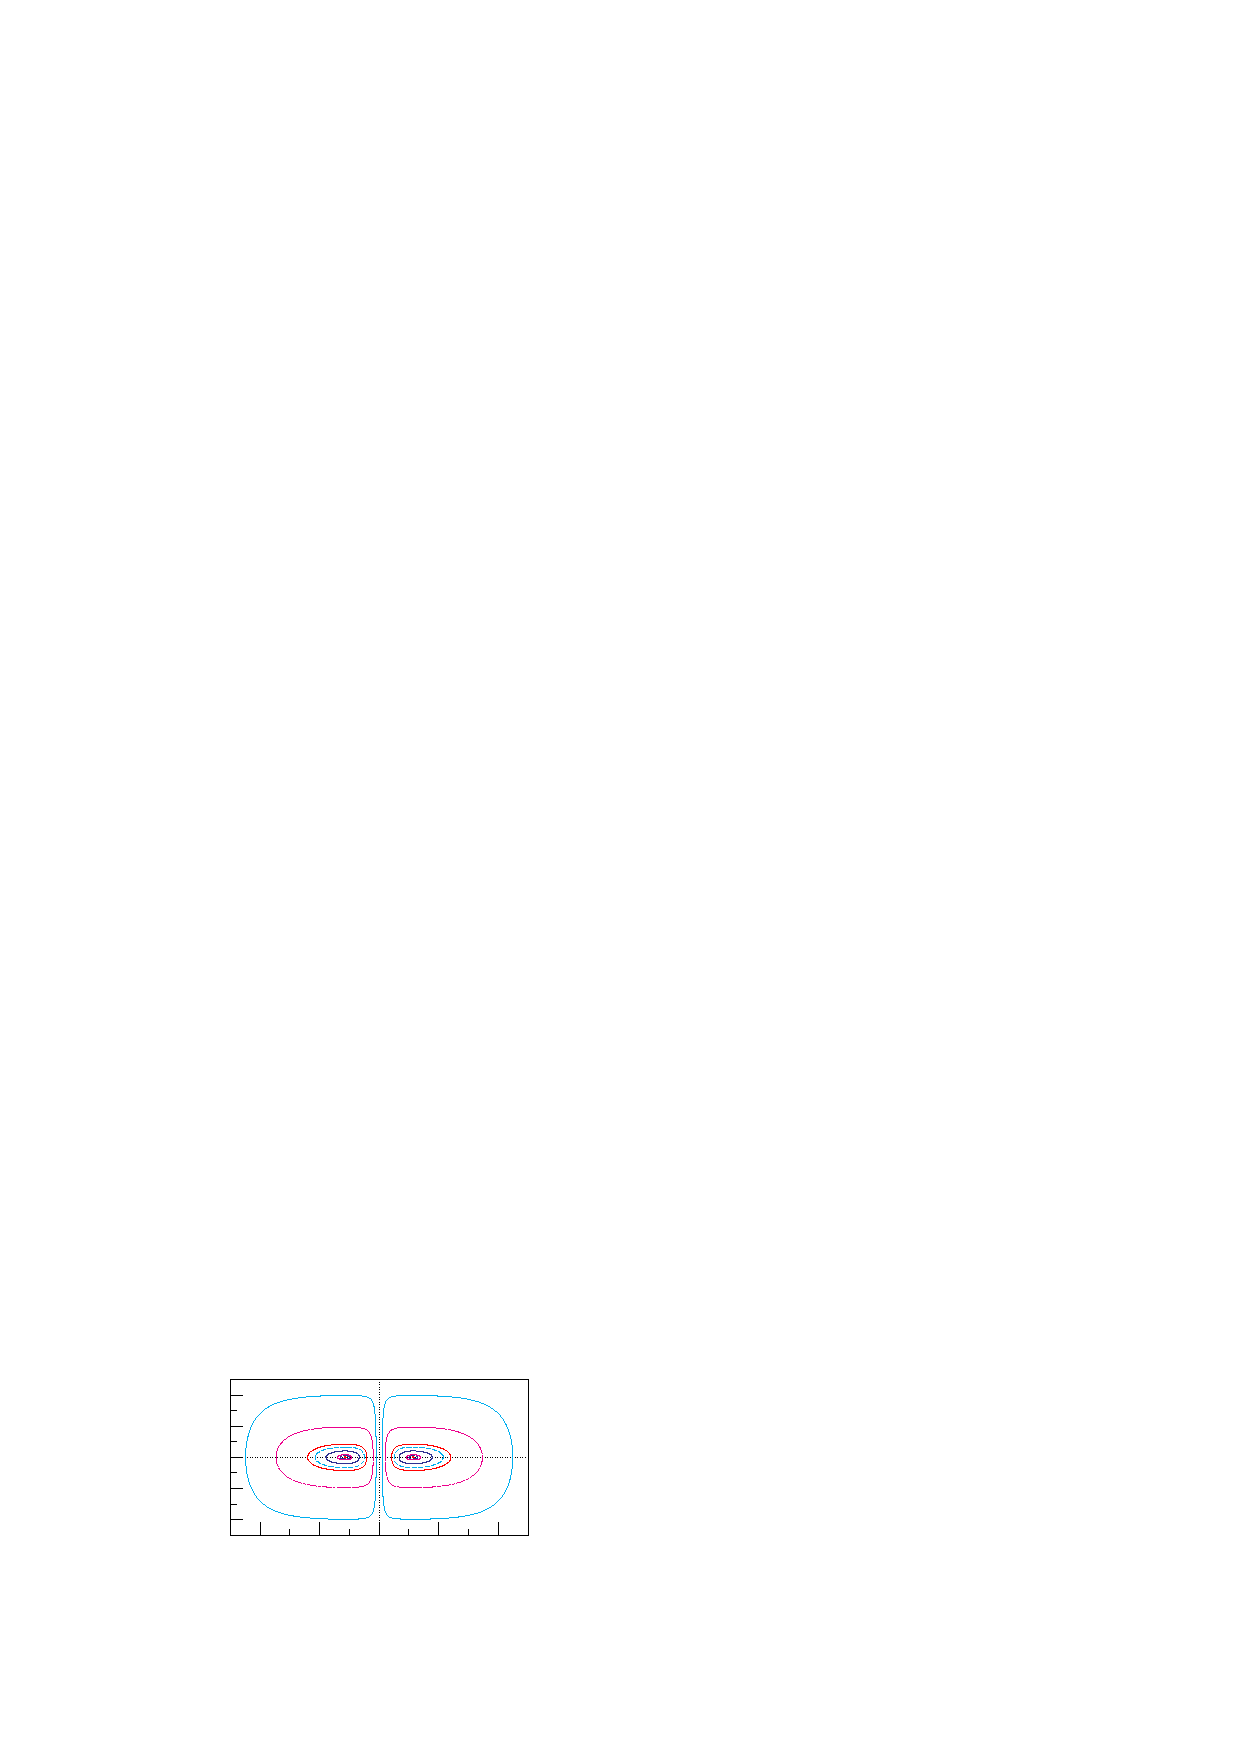
\includegraphics{Images/epslatex/nonaligned_phase}%
\end{picture}%
\begingroup
\setlength{\unitlength}{0.0200bp}%
\begin{picture}(9900,5940)(0,0)%
\put(1650,2024){\makebox(0,0)[r]{\strut{}-2}}%
\put(1650,2772){\makebox(0,0)[r]{\strut{}-1}}%
\put(1650,3520){\makebox(0,0)[r]{\strut{} 0}}%
\put(1650,4268){\makebox(0,0)[r]{\strut{} 1}}%
\put(1650,5016){\makebox(0,0)[r]{\strut{} 2}}%
\put(2640,1100){\makebox(0,0){\strut{}-2}}%
\put(4070,1100){\makebox(0,0){\strut{}-1}}%
\put(5500,1100){\makebox(0,0){\strut{} 0}}%
\put(6930,1100){\makebox(0,0){\strut{} 1}}%
\put(8360,1100){\makebox(0,0){\strut{} 2}}%
\put(550,3520){\rotatebox{90}{\makebox(0,0){\strut{}$p_{\theta}^{}$}}}%
\put(5500,275){\makebox(0,0){\strut{}$\theta$}}%
\end{picture}%
\endgroup
\endinput
 
\end{center}
\caption[Nonaligned equivalent oscillator]{\baselineskip=1.0\normalbaselineskip%
Phase diagram when $\alpha\ne\beta$. On the separatrix given by $\theta=0$ the aligned phase diagram is shown below. The uniform load parameter is $m=1.7$ and the energy levels are $h=3, \, 2, \, 1, \, 0.6$. Thus in both cases the separatrices delineate between classes of chirality.}
\label{fig:nonalignment}
\end{figure}
% 
\begin{figure}[!htbp]
\begin{center}
\input{Images/epslatex/elastica.tex} 
\end{center}
% \vspace*{-0.5cm}
\caption[Planar elastica]{\baselineskip=1.0\normalbaselineskip% 
Phase diagram when $\alpha=\beta=0$. The configurations are given by the load parameter $m=1.7$ and the energies $h=1, \, 0.8, \, 0.6, \, 0.4, \, 0.346, \, 0.2, \, 0,  \, -0.2$}
\label{fig:planar}
\end{figure}
%
\begin{figure}[h!tbp]
\begin{center}
\subfigure[][]{ \input{Images/epslatex/kov_n1.tex} \label{fig:kov_n1} }
\subfigure[][]{ \input{Images/epslatex/kov_n2.tex} \label{fig:kov_n2} }
\subfigure[][]{ %GNUPLOT: LaTeX picture with Postscript
\begin{picture}(0,0)%
\includegraphics{Images/epslatex/kov_n3}%
\end{picture}%
\begingroup
\setlength{\unitlength}{0.0200bp}%
\begin{picture}(9900,6480)(0,0)%
\put(2200,1650){\makebox(0,0)[r]{\strut{}-0.2}}%
\put(2200,2363){\makebox(0,0)[r]{\strut{} 0}}%
\put(2200,3077){\makebox(0,0)[r]{\strut{} 0.2}}%
\put(2200,3790){\makebox(0,0)[r]{\strut{} 0.4}}%
\put(2200,4503){\makebox(0,0)[r]{\strut{} 0.6}}%
\put(2200,5217){\makebox(0,0)[r]{\strut{} 0.8}}%
\put(2200,5930){\makebox(0,0)[r]{\strut{} 1}}%
\put(2475,1100){\makebox(0,0){\strut{} 0}}%
\put(4125,1100){\makebox(0,0){\strut{} 0.5}}%
\put(5775,1100){\makebox(0,0){\strut{} 1}}%
\put(7425,1100){\makebox(0,0){\strut{} 1.5}}%
\put(9075,1100){\makebox(0,0){\strut{} 2}}%
\put(550,3790){\rotatebox{90}{\makebox(0,0){\strut{}$n_{3}$}}}%
\put(5775,275){\makebox(0,0){\strut{}$s$}}%
\end{picture}%
\endgroup
\endinput
 \label{fig:kov_n3} }
\subfigure[][]{ \input{Images/epslatex/kov_m1.tex} \label{fig:kov_m1} }
\subfigure[][]{ \input{Images/epslatex/kov_m2.tex} \label{fig:kov_m2} }
\subfigure[][]{ \input{Images/epslatex/kov_m3.tex} \label{fig:kov_m3} }
\end{center}
\caption[Force and moments of Lagrange and Kovalevskaya homoclinics]{\baselineskip=1.0\normalbaselineskip%
Force and moments of Lagrange (blue) and Kovalevskaya (red) homoclinics when $m=1.70$. The forces and moments were found numerically using a shooting method. Details of the shooting method can be found in the appendix~\ref{chap:numerics}.}
\label{fig:kov}
\end{figure} % 
%
% \section{Action-Angle Formulation} \label{sec:action_angle}
% %
% The Arnol'd-Liouville theorem requires that the level sets be compact for an action-angle formulation, and as has been mentioned this is not the case. Thus in this section, from~\cite{Kehrbaum97a,Arnold89} local action-angle are created and solutions classified from the nature of the action-angle formulation on the $3$-torus. 
% %
% \par
% In order for the Hamilton-Jacobi equation to be separable it is necessary to apply the end force about the $\boldsymbol{d}_{3}$ axis as this director is independent of the angle $\phi$. Thus the system is a single degree of freedom problem. To convert the Hamiltonian from Euler angles into action-angles a generating function $S\left(\theta, I\right)$ which is a solution to the Hamilton-Jacobi equation is introduced
% %
% \begin{align}
% \frac{1}{2}\left( \frac{\partial S}{\partial \theta}\right)^{2} + \frac{1}{2}\left( \frac{ \frac{\partial S}{\partial \psi} - \frac{\partial S}{\partial \phi}\cos\theta }{\sin\theta} \right)^{2} + \frac{\cos\theta}{m^{2}} & = h. \label{eq:general_generating_function}
% \end{align}
% %
% The generating function is then used to find the actions and then the angles
% %
% \begin{equation}
% I_{i} = \frac{1}{2\pi} \oint \frac{\partial S}{\partial q_{i}} \mathrm{d}q_{i}, \quad \mbox{and} \quad \varphi_{i} = \frac{\partial S}{\partial I_{i}} \nonumber 
% \end{equation}
% %
% where the integrals are taken over one cycle of the torus. In order to decouple the actions, the function $S$ is decomposed into three parts
% %
% \begin{align}
% S &= S_{1}\left( I_{1},I_{2},I_{3}, \theta\right) + I_{2} \phi + I_{3}\psi, \nonumber
% \end{align} 
% %
% where the first part is determined by
% %
% \begin{align}
% \frac{\partial S_{1}}{\partial \theta} & = \sqrt{ 2h - \left(\frac{ I_{3} - I_{2} \cos\theta}{\sin^{2}\theta}\right)^{2} - \frac{2\cos\theta}{m^{2}} }. \nonumber
% \end{align}
% %
% Hence, from the substitution $u=\cos\theta$ the nontrivial part of the generating function is given by   
% %
% \begin{align}
% S_{1} & = \int_{u_{1}}^{u} \frac{\sqrt{f\left(u\right) } }{ 1 - u^{2} } \mathrm{d}u, \quad \mbox{where} \quad f\left(u\right) = 2\left(h-u\slash m^{2}\right)\left(1-u^{2}\right) - \left( I_{3} - I_{2} u \right)^{2}, \nonumber
% \end{align}
% %
% where it is assumed that the polynomial $f\left(u\right)$ has three not necessarily unique real roots which satisfy $ -1 < u_{1} \le u_{2} < 1 < u_{3}$. Thus 
% %
% \begin{align}
% f\left(u\right) & = \frac{1}{m^{2}}\left(u-u_{1}\right)\left(u-u_{2}\right)\left(u-u_{3}\right). \nonumber 
% \end{align}
% %
% The actions are given by
% %
% \begin{subequations}
% \begin{align}
% I_{1} & = \frac{1}{\pi} \int_{u_{1}}^{u_{2}} \frac{\sqrt{f\left(u\right) } }{ 1 - u^{2} } \mathrm{d}u, \nonumber \\
% I_{2} & = p_{\psi}, \nonumber \\
% I_{3} & = p_{\phi}, \nonumber 
% \end{align}
% \end{subequations}
% %
% where $I_{1}$ is expressed implicitly as $I_{1} = \tilde{I}_{1}\left(I_{2},I_{3},h\right)$ which in turn allows $h=\tilde{\mathcal{H}}\left(I_{1},I_{2},I_{3}\right)$ to be expressed implicitly. Hence, without loss of generality  $I_{1} = \tilde{I}_{1}\left(I_{2},I_{3},\tilde{\mathcal{H}}\left(I_{1},I_{2},I_{3}\right)\right)$. Thus substituting this expression into the nontrivial part of the generating function yields $S_{1}\left(\theta, I_{1}, I_{2}, I_{3}\right)= \tilde{S}_{1}\left(\theta, I_{2},I_{3}, \tilde{\mathcal{H}}\left(I_{1},I_{2},I_{3}\right)\right) = \tilde{S}_{1}\left(\theta, I_{2},I_{3}, h\right)$. Hence the angles are given by
% %
% \begin{subequations}
% \begin{align}
% \varphi_{1} & = \frac{\partial S}{\partial I_{1} } = \frac{\partial \tilde{S}_{1}}{\partial h} \frac{\partial \tilde{\mathcal{H}}}{\partial I_{1}} = \frac{\partial \tilde{S}_{1}}{\partial h}\omega_{1}, \\ 
% \varphi_{2} & = \frac{\partial S}{\partial I_{2} } = \phi + \frac{\partial S_{1} }{\partial I_{2} } = \phi + \frac{\partial \tilde{S}_{1} }{\partial I_{2} } + \frac{\partial \tilde{S}_{1}}{\partial h} \frac{\partial \tilde{\mathcal{H}} }{\partial I_{2}} = \phi + \frac{\partial \tilde{S}_{1} }{\partial I_{2} } + \frac{\partial \tilde{S}_{1}}{\partial h} \omega_{2}, \\
% \varphi_{3} & = \frac{\partial S}{\partial I_{3} } = \psi + \frac{\partial S_{1} }{\partial I_{3} } = \psi + \frac{\partial \tilde{S}_{1} }{\partial I_{3} } + \frac{\partial \tilde{S}_{1}}{\partial h} \frac{\partial \tilde{\mathcal{H}} }{\partial I_{3}} = \psi + \frac{\partial \tilde{S}_{1} }{\partial I_{3} } + \frac{\partial \tilde{S}_{1}}{\partial h} \omega_{3}.
% \end{align}
% \end{subequations}
% %
% where
% %
% \begin{align}
% \omega_{i} & = \dfrac{\partial \tilde{\mathcal{H}}}{\partial I_{i}}. \nonumber
% \end{align}
% %
% Then, by implicitly differentiation
% %
% \begin{subequations}
% \begin{align}
% \omega_{1} & = \dfrac{\partial \tilde{\mathcal{H}}}{\partial I_{1}} = \left( \dfrac{\partial \tilde{I}_{1}}{\partial h}\right)^{-1}, \\
% \omega_{2} & = \dfrac{\partial \tilde{\mathcal{H}}}{\partial I_{2}} =-\left( \dfrac{\partial \tilde{I}_{1}}{\partial h}\right)^{-1} \dfrac{\partial \tilde{I}_{1}}{\partial I_{2}}, \\
% \omega_{3} & = \dfrac{\partial \tilde{\mathcal{H}}}{\partial I_{3}} =-\left( \dfrac{\partial \tilde{I}_{1}}{\partial h}\right)^{-1} \dfrac{\partial \tilde{I}_{1}}{\partial I_{3}}. 
% \end{align}
% \end{subequations}
% %
% Thus by the definition of the elliptic integrals the frequencies are
% %
% \begin{subequations}
% \begin{align}
% \omega_{1} & = \frac{\pi}{2} m \sqrt{ u_{3} - u_{1} } \frac{1}{K}, \\
% \omega_{2} & = \frac{1}{K} Q_{+}\left(\frac{\pi}{2}\right), \\
% \omega_{3} & = \nu I_{3} - \frac{1}{2K}Q_{-}\left(\frac{\pi}{2}\right)
% \end{align}
% \end{subequations}
% %
% and the angles given by
% %
% \begin{subequations}
% \begin{align}
% \varphi_{1} & = \dfrac{\pi}{K} F\left(v,\sqrt{\dfrac{u_{2}-u_{1}}{u_{3}-u_{1}}}\right), \\
% \varphi_{2} & = \psi + \dfrac{m}{ \sqrt{u_{3}-u_{1}} K} \left( Q_{-}\left(v\right)K - Q_{-}\left(\dfrac{\pi}{2}\right) F\left(v,\sqrt{\dfrac{u_{2}-u_{1}}{u_{3}-u_{1}}} \right) \right), \\
% \varphi_{3} & = \phi - \dfrac{m}{ \sqrt{u_{3}-u_{1}} K} \left( Q_{+}\left(v\right)K - Q_{+}\left(\dfrac{\pi}{2}\right) F\left(v,\sqrt{\dfrac{u_{2}-u_{1}}{u_{3}-u_{1}}} \right) \right)
% \end{align}
% \end{subequations}
% %
% where
% %
% \begin{align}
% Q_{\pm}\left(v\right) & = \dfrac{I_{2}-I_{3}}{1-u_{1}} \Pi \left( v, \dfrac{u_{2}-u_{1}}{1-u_{1}}, \sqrt{ \dfrac{u_{2}-u_{1}}{u_{3}-u_{1}} } \right) \pm  \dfrac{I_{2}+I_{3}}{1+u_{1}}\Pi \left( v, -\dfrac{u_{2}-u_{1}}{1+u_{1}}, \sqrt{ \dfrac{u_{2}-u_{1}}{u_{3}-u_{1}} } \right). \nonumber
% \end{align}
%
% \subsection{Hamiltonian-Hopf Bifurcation}
% %
% Of interest are homoclinic solutions which only occur when $p_{\psi}=p_{\phi}=1$ and $h=1\slash{m^{2}}$. Thus for homoclinic solutions the generating function is given by
% %
% \begin{align}
% S & = S_{1}\left(I_{1},I_{2},I_{3},\theta\right) + \psi I_{2} + \phi I_{3}, \nonumber
% \end{align}
% %
% In contrast to general case~\eqref{eq:general_generating_function} specifying $p_{\psi}=p_{\phi}=1$ then gives have a single root at $u=1$ and two nontrivial roots, 
% %
% \begin{align}
% S_{1} & = \dfrac{2}{m} \int_{?}^{u} \dfrac{ \sqrt{f\left(u\right)} }{ 1 - u^{2} } \, \mathrm{d}s \quad \mbox{where} \quad f\left(u\right) = \left(1-u\right)\left( 2\left(h-u\slash m^{2}\right) - \left(1-u\right)\right). \nonumber
% \end{align}
% %
% However if the energy is set as the homoclinic energy $h=1\slash{m^{2}}$ the polynomial has one nontrivial root and a double root at $u=1$ and the root of the polynomial is simply $u_{1} = u_{0}$. 
% %
% \begin{align}
% S_{1} & = \dfrac{2}{m} \int_{?}^{u} \dfrac{ \sqrt{f\left(u\right)} }{ 1 + u } \, \mathrm{d}s \quad \mbox{where} \quad f\left(u\right) = u - u_{0} \quad \mbox{and} \quad u_{0} = m^{2}\slash 2 - 1. \nonumber
% \end{align}
% %
% The angles are given by
% %
% \begin{subequations}
% \begin{align}
% I_{1} & = \dfrac{1}{\pi m} \int_{ u_{0} }^{1} \dfrac{ u - u_{0} }{ 1 + u } \, \mathrm{d}s = \dfrac{2}{\pi}\sqrt{1-u_{0}}\left( 1 - \tan^{-1}\left(\sqrt{\dfrac{1-u_{0}}{1+u_{0}}}\right) \right) \\
% I_{2} & = p_{\phi}, \\
% I_{3} & = p_{\psi}. 
% \end{align}
% \end{subequations}
% %
% Thus the frequencies of the angle coordinates are given by
% %
% \begin{subequations}
% \begin{align}
% \omega_{1} & = \int_{ u_{0} }^{1} \dfrac{2}{\sqrt{2h\left(1+u\right)-1}}\,\mathrm{d}u = 2\sqrt{1-u_{0}}, \\
% \omega_{2} & = b, \\
% \omega_{3} & = b. 
% \end{align}
% \end{subequations}
% %
% and the angles 
% %
% \begin{subequations}
% \begin{align}
% \varphi_{1} & = b, \\
% \varphi_{2} & = b, \\
% \varphi_{3} & = b. 
% \end{align}
% \end{subequations}
% %
% Hence as $m\rightarrow2$ then the actions $I_{1}$ and $I_{2}$ becomes ill-defined since $u_{0} \rightarrow 0$. \textbf{Thus the system reduces from a three-tori to a one-torus, from a completely integrable system, to a maximally superintegrable system, at the bifurcation point.} 
% %
% \subsection{The Elastica}
% %
% With $p_{\psi}=p_{\phi}=0$ the elastica simply reduces down to 
% %
% \begin{align}
% S & = 4 \sqrt{2} \int_{u_{0}}^{u}  \dfrac{ \sqrt{h-u\slash{m^{2}}} }{1-u^{2}} \, \mathrm{d}u, \quad \mbox{where} \quad u_{0} = hm^2, \nonumber
% \end{align}
% %
% hence the action is 
% %
% \begin{align}
% I & = \dfrac{1}{\pi} \int_{-1}^{ h m^{2} }  \dfrac{ \sqrt{h-u\slash{m^{2}}} }{1-u^{2}} \, \mathrm{d}u , \nonumber\\
% & = \nonumber
% \end{align}
% %
% and the angle is
% %
% \begin{align}
% \varphi & =  \dfrac{\partial S}{\partial I} \nonumber \\
% & = \dfrac{\partial S}{\partial h} \dfrac{\partial h}{\partial I} \nonumber \\
% & = \nonumber
% \end{align}
% %
% Thus as there is no topological change in the tori a bifurcation never occurs for any value of the load parameter.
%
\subsection{Extensibility} \label{subsec:integrable_perturbations}
%
It has been shown by finding explicit solutions without exploiting the Hamiltonian structure, that if an isotropic rod is shearable and extensible then it remains integrable~\cite{Stump00}. In this section, by exploiting the Hamiltonian structure closed form expressions for homoclinic solutions are derived.
%
\par
In the case of isotropic bending $\left(\rho=0\right)$, shear and extension $\left(\sigma=0\right)$ the governing equation can be reduced to a single degree of freedom Hamiltonian system by substituting the moments~\eqref{eq:noncanonical_moment1} and forces~\eqref{eq:kirchhoff_canonical_force} into the Hamiltonian
%
\begin{align}
\mathcal{H} & = \dfrac{1}{2}m_{1}^{2}+\dfrac{1}{2}m_{2}^{2}+\dfrac{1}{2}\left(1+\nu\right)m_{1}^{2} + \dfrac{1}{2m^{2}}\epsilon n_{1}^{2} + \dfrac{1}{2m^{2}}\epsilon n_{2}^{2} + \dfrac{1}{2m^{2}}\epsilon\left(1+\gamma\right)n_{3}^{2} + \dfrac{n_{3}}{m^{2}}. 
\end{align}
%
The Hamiltonian is given by
%
\begin{align}
\mathcal{H}\left( \theta, p_{\theta} \right) & = \frac{1}{2} p_{\theta}^{2} + \frac{1}{2} \left( \frac{p_{\psi}-p_{\phi}\cos\theta}{\sin\theta} \right)^{2} + \frac{1}{2}\left(1+\nu\right)p_{\phi}^{2} + \frac{\cos\theta\left( \epsilon\gamma\cos\theta + 2 \right)}{2m^{2}} + \frac{\epsilon}{2m^{2}} \label{eq:extensible_ham}.
\end{align}
%
The additional constant term $\epsilon \slash 2m^{2}$ is stored energy due to shearability. Thus, when $\alpha=\beta=1$, Hamilton's equations are given by
%
\begin{subequations}
\begin{align}
{\theta}^{\prime} & = p_{\theta}, \\
{p}_{\theta}^{\prime} & = \frac{\sin\theta}{\left(1+\cos\theta\right)^{2}} - \frac{\left(\epsilon\gamma\cos\theta+1\right)\sin\theta}{m^{2}}.
\end{align}
\end{subequations}
%
Solving for fixed points yields the trivial solution $p_{\theta}=0$ and $\sin\theta = 0$ and the nontrivial fixed points
%
\begin{align} 
0 & = \frac{1}{\left(1+\cos\theta\right)^{2}} - \frac{\epsilon\gamma\cos\theta+1}{m^{2}}.
\end{align}
%
Thus, the real solutions to the cubic
%
\begin{align}
0 & = \epsilon \gamma \cos^{3}\theta + \cos^{2}\theta + \epsilon \gamma \cos\theta + 1-m^{2}
\end{align}
%
determine the configurations for helices and hence the buckling load. It should be noted that only a single helix exists when $\epsilon\gamma$ is small since solutions to the equation are required to be real-valued angles and the equation has two imaginary roots and a single real root. The condition for three real roots is given by
%
\begin{align}
\left(1-\dfrac{1}{3}\dfrac{1}{\epsilon\gamma}\right)^{3}\slash{27} + \left(\dfrac{1}{\epsilon\gamma}\right)^{2}\left(\dfrac{2}{27}\left(\dfrac{1}{\epsilon\gamma}\right)^{2} + \dfrac{2}{3} -m^{2} \right)^{2}\slash{4} \ge 0
\end{align}
%
% Substituting the real root of the cubic into the formula for a helix yields the buckling value for the extensible rod. 
Previously the analysis of the buckling of an extensible rod had been derived by linearisation~\cite{Champneys97b}. 
%
\par
Nontrivial solutions can be found from the integral
%
\begin{align}
s & = \int_{u\left(0\right)}^{u\left(s\right)} \dfrac{\mathrm{d}u}{ \sqrt{2\left( h-u\left(u \epsilon\gamma\slash 2 +1\right)\slash m^{2}\right)\left(1-u^{2}\right)-\left(\alpha-\beta u\right)^{2} } }.
\end{align}
%
The homoclinic now has energy given by 
%
\begin{align}
h & = \dfrac{1}{m^{2}}\left(1+\dfrac{\epsilon\gamma}{2}\right) \nonumber
\end{align}
%
which, along with the torque condition $\alpha=\beta=1$ yields the integral
%
\begin{align}
s & = \int_{u\left(0\right)}^{u\left(s\right)} \dfrac{\mathrm{d}u}{ \left(1-u\right)\sqrt{ \epsilon\gamma \left(u+1\right)^{2} \slash m^{2} + 2\left(u+1\right)\slash m^{2} + 1 } }. \nonumber
\end{align}
%
The integral can be expressed in the form
%
\begin{align}
s & = \dfrac{m}{\sqrt{\epsilon\gamma}} \int_{u\left(0\right)}^{u\left(s\right)} \dfrac{ \mathrm{d}u }{ \left(1-u\right) \sqrt{ f\left(u\right) } }, \quad \mbox{where} \quad f\left(u\right) = u^{2} + 2 u\left(1+\dfrac{1}{\epsilon\gamma}\right) + 1 + \dfrac{2}{\epsilon\gamma} -\dfrac{m^{2}}{\epsilon\gamma}. \nonumber
\end{align}
%
The quadratic $f\left(u\right)$ has roots
%
\begin{align}
u_{\pm} & = -\left(1+\dfrac{1}{\epsilon\gamma}\right) \pm \dfrac{1}{\epsilon\gamma}\sqrt{ 1 + \epsilon \gamma m^{2} }, \nonumber
\end{align}
%
which in the limit of small extensibility, that is $\epsilon \gamma m^{2} \ll 1$, yields
%
\begin{align}
u_{+} & = \dfrac{m^{2}}{2} - 1 - \dfrac{1}{8}\left( \epsilon\gamma m^{2} \right)^{2} + \frac{1}{16}\left( \epsilon\gamma m^{2} \right)^{3} + \mathcal{O}\left(\epsilon^{4}\right), \nonumber \\ 
u_{-} & = -1 - \dfrac{m^{2}}{2} - \dfrac{2}{\epsilon\gamma} + \dfrac{1}{8}\left( \epsilon\gamma m^{2} \right)^{2} - \frac{1}{16}\left( \epsilon\gamma m^{2} \right)^{3} + \mathcal{O}\left(\epsilon^{4}\right). \nonumber 
\end{align}
%
So that the roots scale as perturbations of the inextensible rod, that is $u_{+} \sim u_{0}$ and $u_{-} \sim -1$. Hence the limits of integration become
%
\begin{align}
s & = \dfrac{m}{\sqrt{\epsilon\gamma}}\int_{u_{+}}^{u\left(s\right)}\dfrac{\mathrm{d}z}{\left(1-u\right)\sqrt{\left(u+u_{-}\right)\left( u-u_{+}\right)}}. \nonumber
\end{align}
%
On the substitution $u = -u_{-} + \left(u_{-}+u_{+}\right)\cosh^{2} z $ the integral becomes
%
\begin{align}
s & = \dfrac{2m}{\left(1+u_{-}\right)\sqrt{\epsilon\gamma}} \int_{0}^{z\left(s\right)} \dfrac{ \mathrm{d}z }{ 1 - k \cosh^{2}z } , \quad \mbox{with} \quad k = \dfrac{u_{-}+u_{+}}{1+u_{-}},
\end{align}
%
where
%
\begin{align}
z\left(s\right) & = \cosh^{-1} \sqrt{ \dfrac{u\left(s\right)-u_{-}}{u_{+}+u_{-}} } \nonumber
\end{align}
%
and the integral is given by
%
\begin{align}
\int \dfrac{\mathrm{d}z}{1 - k \cosh^{2} z} & = \dfrac{-2}{\sqrt{k^{2}-1}} \tan^{-1}\left( \sqrt{\dfrac{k+1}{k-1}}\tanh \dfrac{z}{2} \right).  \label{eq:ext_homoclinic}
\end{align}
%
In the limit of $\epsilon \rightarrow 0$ the Kirchhoff homoclinic~\eqref{eq:isotropic_homoclinic} is recovered. The derivative of the angle $\psi$ is given by
%
\begin{align}
{\psi}^{\prime} & = \frac{1}{1+\cos\theta}. \label{eq:extensibility_psi}
\end{align} 
%
\par
The evolutions of the Euler angles and their conjugtaes are quantatively the same as those displayed in figures~\ref{fig:evolutions} and~\ref{fig:omegas} and so are not presented.
% 
\section{Nonintegrable Perturbations} \label{sec:nonintegrable_perturbations}
%
In this section anisotropy and initial curvature~\cite{Heijden98a,Champneys97a} are shown to destroy integrability.
%
\par
For material perturbations the constitutive relations change but the force and moment balance remain the same. Thus, the Casimirs remain the same, and hence the reduction holds.  Both cases have been studied before but in a different formulation using Deprit variables.
%
\par
The Hamiltonian system now takes the general form
%
\begin{align}
\mathcal{H}_{\epsilon}\left(\theta,\phi,p_{\theta},p_{\phi},p_{\psi}\right) & = \mathcal{H}_{0}\left(\theta,p_{\theta},p_{\phi},p_{\psi}\right) + \epsilon \mathcal{H}_{1}\left(\theta,\phi,p_{\theta},p_{\phi},p_{\psi}\right),
\end{align} 
%.
where the unperturbed Hamiltonian is given by~\eqref{eq:two_dim_ham}, the unperturbed homoclinic by~\eqref{eq:isotropic_homoclinic} and the frequency of the angle $\phi$ is given by

\begin{align}
\omega_{0} & = \dfrac{\partial \mathcal{H}_{0}}{\partial p_{\phi}} = \nu + \dfrac{2}{m^{2} + \left(4+m^{2}\right)\tanh^{2}\left(\dfrac{\sqrt{4+m^{2}}}{2m}s\right)}. \label{eq:Omega_0_explicit}
\end{align}
%
Thus when $\nu\ge0$ then $\omega_{0} \ge \delta > 0$ for a small, fixed $\delta$. The equilibrium point~\eqref{eq:trivial_fp} from which the homoclinic eminates from is a hyperbolic saddle. Thus Mel'nikov's method, as described in \S\ref{sec:melnikov_thm}, may be applied to test for the breakup of integrability due to the loss of the Lagrange integral $p_{\phi}$.
%
% \par
% It should be noted that the canonical system is still invariant under the action of $S^{1}$, thus the modified version of Mel'nikov's method, as described in, is required. Note that in all cases considered in this section the system is perturbed by a single term of order $\epsilon$. The Mel'nikov analysis still only provides a first order approximation to the rate of splitting of the unstable and stable manifolds, as the action-angle variables can still expressed as a series in the perturbation parameters.
%
\par
The partial derivatives of the unperturbed Hamiltonian and angular frequency evaluated at the homoclinic energy level are given by
%
\begin{subequations}
\label{eq:partials}
\begin{align}
\dfrac{\partial \mathcal{H}_{0}}{\partial \theta} & = \dfrac{\sin\theta}{\left(1+\cos\theta\right)^{2}} - \dfrac{\sin\theta}{m^{2}}, \\
\dfrac{\partial \mathcal{H}_{0}}{\partial p_{\theta}} & = p_{\theta}, \\
\dfrac{\partial \omega_{0}}{\partial \theta} & = \dfrac{\sin\theta}{\left(1+\cos\theta\right)^{2}}, \\
\dfrac{\partial \omega_{0}}{\partial p_{\theta}} & = 0 .
\end{align}
\end{subequations}
%
That $p_\theta$ is an odd function and $\theta$ and $\omega_{0}$ are even functions will be used to simplify the Mel'nikov integral.
% 
\subsection{Anisotropy} \label{subsec:anisotropy}
%
When the rod is linearly elastic, unshearable, inextensible, initially straight and anisotropic the constitutive relations are given by
%
\begin{align}
\mathcal{W}\left(\mathsf{u}\right) & = \frac{1}{2} B_{1} u_{1}^{2} + \frac{1}{2} B_{2} u_{1}^{2} + \frac{1}{2} C u_{3}^{2}. 
\end{align}
%
The nondimensional Hamiltonian is given by
%
\begin{align}
\mathcal{H} & = \frac{1}{2}p_{\theta}^{2} +  \left(\frac{p_{\psi}-p_{\phi}\cos\theta}{\sin\theta}\right)^{2} + \frac{1}{2}\left(1+\nu\right)p_{\phi}^{2} + \frac{\cos\theta}{m^{2}} \nonumber \\ 
& \hspace{3.0cm} + \frac{\rho}{2} \left( p_{\theta}\sin\phi - \cos\phi\left(\frac{p_{\psi}-p_{\phi}\cos\theta}{\sin\theta}\right) \right)^{2}.
\end{align}
%
Hamilton's equations are
%
\begin{subequations}
\label{eq:dot}
\begin{align}
{\theta}^{\prime} & = p_{\theta} + \rho\sin\phi\left( p_{\theta}\sin\phi - \cos\phi \left( \frac{p_{\psi}-p_{\phi}\cos\theta}{\sin\theta} \right) \right), \label{eq:dot_theta} \\
{\phi}^{\prime} & = \left(1+\nu\right) p_{\phi} - \cos\theta\left( \frac{p_{\psi}-p_{\phi}\cos\theta}{\sin^{2}\theta} \right) \nonumber \\
& \hspace{1.5cm} + \rho\frac{\cos\phi\cos\theta}{\sin\theta}\left( p_{\theta}\sin\phi - \cos\phi\left( \frac{p_{\psi}-p_{\phi}\cos\theta}{\sin\theta} \right) \right), \label{eq:dot_phi} \\
{\psi}^{\prime} & = \left(\frac{p_{\psi}-p_{\phi}\cos\theta}{\sin^{2}\theta}\right) - \rho\frac{\cos\phi}{\sin\theta}\left( p_{\theta}\sin\phi - \cos\phi\left(\frac{p_{\psi}-p_{\phi}\cos\theta}{\sin\theta}\right) \right), \label{eq:dot_psi}\\
{p}_{\theta}^{\prime} & = \frac{ \sin\theta }{ m^{2} } - \left( \frac{p_{\phi}-p_{\psi}\cos\theta}{\sin\theta} \right)\left( \frac{p_{\psi}-p_{\phi}\cos\theta}{\sin^{2}\theta} \right)\nonumber \\
& \hspace{1.5cm}- \rho\cos\phi\left( \frac{p_{\psi}-p_{\phi}\cos\theta}{\sin^{2}\theta} \right)\left( p_{\theta}\sin\phi - \cos\phi\left(\frac{p_{\phi}-p_{\psi}\cos\theta}{\sin\theta}\right)\right), \label{eq:dot_p_theta} \\  
{p}_{\phi}^{\prime} & = \rho\left(p_{\theta}\cos\phi+\sin\phi\left(\frac{p_{\phi}-p_{\psi}\cos\theta}{\sin\theta}\right) \right)\left(p_{\theta}\sin\phi - \cos\phi\left(\frac{p_{\phi}-p_{\psi}\cos\theta}{\sin\theta}\right)\right),\label{eq:dot_p_phi} \\
{p}_{\psi}^{\prime} & = 0. \label{eq:dot_p_psi}
\end{align}
\end{subequations}
%
Thus the six-dimensional noncanonical system~\eqref{eq:kirchhoff} is reduced to a four-dimensional canonical Hamiltonian system. Expressing $\phi\left(s\right) = \bar\phi\left(s\right)+\phi_{0}$ the perturbation to the Hamiltonian is of the form
%
\begin{align}
\mathcal{H}_{1} & = \dfrac{1}{2}\cos2\phi_{0} \left( \cos2\bar{\phi} \left(p_{\theta}^{2}+ \dfrac{1-\cos\theta}{1+\cos\theta}\right) - p_{\theta}\sin2\bar{\phi}\left(\dfrac{1-\cos\theta}{\sin\theta}\right)\right)  \nonumber \\
& \hspace{1.0cm} - \dfrac{1}{2}\sin2\phi_{0} \left( \sin2\bar{\phi} \left(p_{\theta}^{2} + \dfrac{1-\cos\theta}{1+\cos\theta}\right) + p_{\theta}\cos2\bar{\phi}\left(\dfrac{1-\cos\theta}{\sin\theta}\right)\right) \nonumber \\
& \hspace{2.0cm} - \dfrac{1}{2}p_{\theta}^{2} + \dfrac{1}{2}\left(\dfrac{1-\cos\theta}{1+\cos\theta}\right).
\end{align}
%
The partial derivatives of the perturbation are given by
%
\begin{subequations}
\label{eq:H1_partial_anisotropic}
\begin{align}
\dfrac{\partial \mathcal{H}_{1}}{\partial \theta} & = \dfrac{1}{2}p_{\theta}\left(\cos2\phi_{0}\cos2\bar{\phi} - \sin2\phi_{0}\sin2\bar{\phi}-1\right)\nonumber \\
& \hspace{1.0cm} + \left(1-\dfrac{1}{2}\left(\cos2\phi_{0}\cos2\bar{\phi}-\sin2\phi_{0}\sin2\bar{\phi}\right)\right)\left(\dfrac{1-\cos\theta}{\left(1+\cos\theta\right)\sin\theta} \right), \\
\dfrac{\partial \mathcal{H}_{1}}{\partial p_{\theta}} & = \dfrac{1}{2} p_{\theta}\left(\cos2\phi_{0}\cos2\bar{\phi}-\sin2\phi_{0}\sin2\bar{\phi}-1\right) \nonumber \\
& \hspace{1.0cm} - \dfrac{1}{2}\left(\sin2\phi_{0}\cos2\bar{\phi}-\cos2\phi_{0}\sin2\bar{\phi}\right)\left( \dfrac{1-\cos\theta}{\sin\theta} \right).
\end{align}
\end{subequations}
%
Hence the Mel'nikov integral is given by
%
\begin{align}
\mathcal{M}_{h}\left(\phi_{0}\right) & = \sin\phi_{0}\int^{+\infty}_{-\infty} A\left(s\right)\,\mathrm{d}s + \cos\phi_{0}\int^{+\infty}_{-\infty} B\left(s\right)\,\mathrm{d}s + \int^{+\infty}_{-\infty} C\left(s\right)\,\mathrm{d}s
\end{align}
%
where
%
\begin{subequations}
\begin{align}
A\left(s\right) & = \dfrac{1}{2}\left( \dfrac{1+\cos\theta}{m^{2}} + \dfrac{1}{1+\cos\theta} +p_{\theta}^{2}\right)\left(p_{\theta}\sin\theta\sin2\bar\phi-\left(1-\cos\theta\right)\cos2\bar\phi\right) \nonumber \\
& \hspace{1.0cm} + \dfrac{1}{2}p_{\theta}^{2}\cos\theta\left( \cos2\bar\phi + \sin2\bar\phi\left(\dfrac{1-\cos\theta}{\sin\theta}\right) \right), \\
B\left(s\right) & = \dfrac{1}{2}\left( \dfrac{1+\cos\theta}{m^{2}} + \dfrac{1}{1+\cos\theta} +p_{\theta}^{2}\right)\left(p_{\theta}\sin\theta\cos2\bar\phi-\left(1-\cos\theta\right)\sin2\bar\phi\right) \nonumber \\
& \hspace{1.0cm} + \dfrac{1}{2}p_{\theta}^{2}\cos\theta\left( \sin2\bar\phi - \cos2\bar\phi\left(\dfrac{1-\cos\theta}{\sin\theta}\right) \right), \\
C\left(s\right) & = \dfrac{1}{2} p_{\theta} \left( \dfrac{1-\cos\theta}{\sin\theta} + \dfrac{1+\cos\theta}{m^{2}} + \dfrac{1}{1+\cos\theta} + p_{\theta}^{2} \right).
\end{align}
\end{subequations}
%
Then the condition for simple zeroes is given by 
%
\begin{align}
\left| \dfrac{c}{ \sqrt{ a^{2} + b^{2} } } \right| \le 1 
\end{align}
% 
where
% 
\begin{align}
a = \int_{-\infty}^{\infty}A\left(s\right)\,\mathrm{d}s, \quad b = \int_{-\infty}^{\infty}B\left(s\right)\,\mathrm{d}s \quad \mbox{and} \quad c = \int_{-\infty}^{\infty}C\left(s\right)\,\mathrm{d}s. \nonumber
\end{align}
%
The Mel'nikov integral is evaluated in figure~\ref{fig:Mel_aniso_1.75} for a variety of values for $m$. The curves show that generically the Mel'nikov integral has simple zeroes.
%
\begin{figure}[!htbp]
\begin{center}
%GNUPLOT: LaTeX picture with Postscript
\begin{picture}(0,0)%
\includegraphics{Images/epslatex/Mel_aniso_m.eps}%
\end{picture}%
\begingroup
\setlength{\unitlength}{0.0200bp}%
\begin{picture}(18000,6480)(0,0)%
\put(2200,1650){\makebox(0,0)[r]{\strut{}-2.5}}%
\put(2200,2078){\makebox(0,0)[r]{\strut{}-2}}%
\put(2200,2506){\makebox(0,0)[r]{\strut{}-1.5}}%
\put(2200,2934){\makebox(0,0)[r]{\strut{}-1}}%
\put(2200,3362){\makebox(0,0)[r]{\strut{}-0.5}}%
\put(2200,3790){\makebox(0,0)[r]{\strut{} 0}}%
\put(2200,4218){\makebox(0,0)[r]{\strut{} 0.5}}%
\put(2200,4646){\makebox(0,0)[r]{\strut{} 1}}%
\put(2200,5074){\makebox(0,0)[r]{\strut{} 1.5}}%
\put(2200,5502){\makebox(0,0)[r]{\strut{} 2}}%
\put(2200,5930){\makebox(0,0)[r]{\strut{} 2.5}}%
\put(17175,1100){\makebox(0,0){\strut{}$2\pi$}}%
\put(13500,1100){\makebox(0,0){\strut{}$3\pi\slash{2}$}}%
\put(9825,1100){\makebox(0,0){\strut{}$\pi$}}%
\put(6150,1100){\makebox(0,0){\strut{}${\pi}\slash{2}$}}%
\put(2475,1100){\makebox(0,0){\strut{}0}}%
\put(550,3790){\makebox(0,0){\strut{}\rotatebox{90}{$\mathcal{M}^{\left(1\right)}_{h}\left(\phi_{0}\right)$} }}%
\put(9825,275){\makebox(0,0){\strut{}$\phi_0$}}%
%
%\put(6500,2250){\makebox(0,0){\strut{} {\tiny $m=1.70$} }}%
%\put(9000,5250){\makebox(0,0){\strut{} {\tiny $m=1.80$} }}%
\end{picture}%
\endgroup
\endinput
 \label{fig:Mel_aniso_1.75} 
\end{center}
\caption[Anisotropic Mel'nikov integral]{Mel'nikov integral for anisotropic rod with $\nu=1\slash{3}$ and $m = 1.70$, $1.72$, $1.74$, $1.76$, $1.78$, $1.80$ at the homoclinic energy level.}
\end{figure}
% 
\subsection{Initial Curvature} \label{subsec:curvature}
%
For a rod with initial curvature the constitutive relationship take the form
%
\begin{align}
\mathcal{W}\left(\mathsf{u}\right) & = \frac{B_{1}}{2}u_{1}^{2}-u_{0}u_{1} + \frac{B_{1}}{2}u_{2}^{2} + \frac{C}{2}u_{3}^{2}.
\end{align} 
% 
In the initially curved case the nondimensionalised Hamiltonian is given by
%
\begin{align}
\mathcal{H} & = \frac{1}{2}p_{\theta}^{2} + \frac{1}{2}\left(1+\nu\right)p_{\phi}^{2} + \frac{1}{2}\left( \frac{ p_{\psi} - p_{\phi}\cos\theta }{\sin\theta}\right)^{2} + \frac{\cos\theta}{m^{2}} \nonumber \\ 
& \hspace{4.0cm} + \frac{1}{2}\kappa_{0} \left( p_{\theta}\sin\phi - \cos\phi \left( \frac{p_{\psi}-p_{\phi}\cos\theta}{\sin\theta} \right) \right). 
\end{align} 
%
It is interesting to observe that the perturbation for initial curvature is the square root of the perturbation for anisotropy. The governing equations are
%
\begin{subequations}
\label{eq:curv}
\begin{align}
{\theta}^{\prime} & = p_{\theta} + \kappa_{0}\sin\phi, \label{eq:curv_theta} \\
{\phi}^{\prime} & = \left(1+\nu\right) p_{\phi} - \cos\theta\left( \frac{p_{\psi}-p_{\phi}\cos\theta}{\sin^{2}\theta} \right) + \kappa_{0}\frac{\cos\theta\cos\phi}{\sin\theta}, \label{eq:curv_phi} \\
{\psi}^{\prime} & = \left(\frac{p_{\psi}-p_{\phi}\cos\theta}{\sin^{2}\theta}\right) - \kappa_{0}\frac{\cos\phi}{\sin\theta}, \label{eq:curv_psi} \\
{p}_{\theta}^{\prime} & = \frac{ \sin\theta }{ m^{2} } - \left( \frac{p_{\phi}-p_{\psi}\cos\theta}{\sin\theta} \right)\left( \frac{p_{\psi}-p_{\phi}\cos\theta}{\sin^{2}\theta} \right) - \kappa_{0}\cos\phi\left( \frac{p_{\phi}-p_{\psi}\cos\theta}{\sin^{2}\theta} \right), \label{eq:curv_p_theta} \\ 
{p}_{\phi}^{\prime} & = -\kappa_{0} \left( p_{\theta}\cos\phi + \sin\phi\left(\frac{p_{\psi}-p_{\phi}\cos\theta}{\sin\theta} \right)\right), \label{eq:curv_p_phi} \\
{p}_{\psi}^{\prime} & = 0. \label{eq:curv_p_psi} 
\end{align}
\end{subequations}
%
The perturbation to the Hamiltonian is given by
%
\begin{align}
\mathcal{H}_{1} & = \sin\phi_{0}\left( p_{\theta}\cos\bar\phi + \sin\bar{\phi}\left(\dfrac{1-\cos\theta}{\sin\theta}\right) \right) + \cos\phi_{0}\left( p_{\theta}\sin\bar\phi - \cos\bar{\phi}\left(\dfrac{1-\cos\theta}{\sin\theta}\right) \right). \nonumber 
\end{align}
%
The partial derivatives of the perturbation to the Hamiltonian are given by
%
\begin{subequations}
\label{eq:H1_partial_curved}
\begin{align}
\dfrac{\partial \mathcal{H}_{1}}{\partial \theta} & = \dfrac{\sin\phi_{0}\sin\bar{\phi}-\cos\phi_{0}\cos\bar{\phi}}{1+\cos\theta}, \\
\dfrac{\partial \mathcal{H}_{1}}{\partial p_{\theta}} & = \sin\phi_{0}\cos\bar{\phi} + \sin\bar{\phi}\cos\phi_{0}.
\end{align}
\end{subequations}
%
Hence, substituting the results~\eqref{eq:partials} and~\eqref{eq:H1_partial_curved} into the bracket~\eqref{eq:melnikov_bracket} and then substituting the homoclinic solutions~\eqref{eq:isotropic_homoclinic} into the resulting expression gives a Mel'nikov function of the form
%
\begin{align}
\mathcal{M}_{h}\left(\phi_{0}\right) & = \sin\phi_{0}\int^{+\infty}_{-\infty} A\left(s\right) \, \mathrm{d}s + \cos\phi_{0}\int^{+\infty}_{-\infty} B\left(s\right) \, \mathrm{d}s,
\end{align}
%
where
%
\begin{subequations}
\begin{align}
A\left(s\right) & = p_{\theta}\cos\theta\sin\bar\phi - \left( \dfrac{1+\cos\theta}{m^{2}} + \dfrac{1}{1+\cos\theta} + p_{\theta}^{2} \right)\sin\theta\cos\bar\phi \\
B\left(s\right) & = p_{\theta}\cos\theta\cos\bar\phi + \left( \dfrac{1+\cos\theta}{m^{2}} + \dfrac{1}{1+\cos\theta} + p_{\theta}^{2} \right)\sin\theta\sin\bar\phi
\end{align}
\end{subequations}
%
It follows from the reversibilities of the homoclinic solutions that the Mel'nikov function can be simplified over the half range 
%
\begin{align}
\mathcal{M}_{h}\left(\phi_{0}\right) & = 2\cos\phi_{0}\int^{+\infty}_{0}\sin\bar\phi\sin\theta\left(\dfrac{1+\cos\theta}{m^{2}} + \dfrac{1}{1+\cos\theta} + p_{\theta}^{2}\right) \, \mathrm{d}s \nonumber \\
& \hspace{1.5cm} + 2\sin\phi_{0}\int^{+\infty}_{0}p_{\theta}\cos\theta\sin\bar\phi \, \mathrm{d}s. 
\end{align}
%
\par
In contrast to the anisotropic case, there is no constant term in the Mel'nikov function, thus there are no bounds on the existence of transverse intersections of the stable and unstable manifolds. In figure~\ref{fig:poincare_curv} Poincar\'e sections which show the loss of integrability are presented. 
%
\par
The Poincar\'e sections were computed by fixing the integrals $p_{\psi}=1$ and placing the initial conditions were placed near the (unpertubed) saddle: $p_{\theta}=\theta=1\slash1000$ with $p_{\phi}=1$ and solving $\mathcal{H}\left(\theta,p_\theta,\phi,p_{\phi}\right)=h$ for $\phi$. The section itself was defined by $\cos\phi=0$.
%
\begin{figure}[h!tbp]
\label{fig:poincare_curv}
\begin{center}
\subfigure[][$\kappa_{0}=0.001$]{ \input{Images/epslatex/Poincare_kappa_0.001.tex} \label{fig:curv_poincare_0.001} }
\subfigure[][$\kappa_{0}=0.005$]{ \input{Images/epslatex/Poincare_kappa_0.005.tex} \label{fig:curv_poincare_0.005} }
\subfigure[][$\kappa_{0}=0.01$]{  %GNUPLOT: LaTeX picture with Postscript
\begin{picture}(0,0)%
\includegraphics{Images/epslatex/Poincare_kappa_0.01.eps}%
\end{picture}%
\begingroup
\setlength{\unitlength}{0.0200bp}%
\begin{picture}(9900,6480)(0,0)%
\put(2200,5502){\makebox(0,0)[r]{\strut{} 0.4}}%
\put(2200,4646){\makebox(0,0)[r]{\strut{} 0.2}}%
\put(2200,3790){\makebox(0,0)[r]{\strut{} 0}}%
\put(2200,2934){\makebox(0,0)[r]{\strut{}-0.2}}%
\put(2200,2078){\makebox(0,0)[r]{\strut{}-0.4}}%
\put(9075,1100){\makebox(0,0){\strut{} 1.6}}%
\put(8250,1100){\makebox(0,0){\strut{} 1.4}}%
\put(7425,1100){\makebox(0,0){\strut{} 1.2}}%
\put(6600,1100){\makebox(0,0){\strut{} 1}}%
\put(5775,1100){\makebox(0,0){\strut{} 0.8}}%
\put(4950,1100){\makebox(0,0){\strut{} 0.6}}%
\put(4125,1100){\makebox(0,0){\strut{} 0.4}}%
\put(3300,1100){\makebox(0,0){\strut{} 0.2}}%
\put(2475,1100){\makebox(0,0){\strut{} 0}}%
\put(550,3790){\rotatebox{90}{\makebox(0,0){\strut{}$p_{\theta}$}}}%
\put(5775,275){\makebox(0,0){\strut{}$\theta$}}%
\end{picture}%
\endgroup
\endinput
 \label{fig:curv_poincare_0.010} }
\subfigure[][$\kappa_{0}=0.015$]{ \input{Images/epslatex/Poincare_kappa_0.015.tex} \label{fig:curv_poincare_0.015} }
\subfigure[][$\kappa_{0}=0.02$]{  %GNUPLOT: LaTeX picture with Postscript
\begin{picture}(0,0)%
\includegraphics{Images/epslatex/Poincare_kappa_0.02.eps}%
\end{picture}%
\begingroup
\setlength{\unitlength}{0.0200bp}%
\begin{picture}(9900,6480)(0,0)%
\put(2200,2078){\makebox(0,0)[r]{\strut{}-0.4}}%
\put(2200,2934){\makebox(0,0)[r]{\strut{}-0.2}}%
\put(2200,3790){\makebox(0,0)[r]{\strut{} 0}}%
\put(2200,4646){\makebox(0,0)[r]{\strut{} 0.2}}%
\put(2200,5502){\makebox(0,0)[r]{\strut{} 0.4}}%
\put(2475,1100){\makebox(0,0){\strut{} 0}}%
\put(3355,1100){\makebox(0,0){\strut{} 0.2}}%
\put(4235,1100){\makebox(0,0){\strut{} 0.4}}%
\put(5115,1100){\makebox(0,0){\strut{} 0.6}}%
\put(5995,1100){\makebox(0,0){\strut{} 0.8}}%
\put(6875,1100){\makebox(0,0){\strut{} 1}}%
\put(7755,1100){\makebox(0,0){\strut{} 1.2}}%
\put(8635,1100){\makebox(0,0){\strut{} 1.4}}%
\put(550,3790){\rotatebox{90}{\makebox(0,0){\strut{}$p_{\theta}$}}}%
\put(5775,275){\makebox(0,0){\strut{}$\theta$}}%
\end{picture}%
\endgroup
\endinput
 \label{fig:curv_poincare_0.020} }
\subfigure[][$\kappa_{0}=0.05$]{  \input{Images/epslatex/Poincare_kappa_0.05.tex} \label{fig:curv_poincare_0.050} }
\end{center}
% \vspace*{-0.5cm}
\caption[Poincar\'e sections for initially curved rods on homoclinic energy level]{\baselineskip=1.0\normalbaselineskip%
Poincar\'e sections for initially curved rods on the unperturbed homoclinic energy level $h=1\slash m^{2}$ for varying levels of $\kappa_{0}$ on the hypersection determined by $\cos\phi=0$.}
\end{figure} % 
%
\section{Consequences of Nonintegrability} \label{sec:conseq} %
%
Mel'nikov analysis shows the existence of Smale horsehoes, which elegantly describe sensitivity to initial conditions. Arbitarily small changes in the perturbation $\mathcal{H}_{1}$ grow exponentially along the arclength until they reach the same order of magnitude as the field variables $\left(\mathsf{n},\mathsf{m}\right)$. A multiplicity of multimodal solutions now exists~\cite{Champneys96b}. But the system has a well defined bifurcation structure determined by acculumation and coalescence rules~\cite{Heijden98a,Champneys97a}. The computation and continuation of multimodal solutions between two fixed points is well known, so detail is presented in appendix~\S\ref{chap:numerics}. The purpose of this section is to present evidence to support and to contrast with latter results. %
% 
\par
Multimodal solutions can be described by a number of distinct primary localisations separated by a number of smaller oscillations. Bimodals are denoted by $\left(P_{i},n,P_{j}\right)$ where the total number of smaller oscillations separating the primary localisations is denoted as $n$. Each oscillation is a quarter turn the rod makes between modes. When $n$ is small then the correspondence between a primary homoclinic and a mode of the bimodal is not immediately evident but when $n$ is large the correspondence becomes clear as the two modes \emph{accumulate} onto the primary homoclinics. Accumulation results can be seen in table~\ref{tab:shooting_rho_bimodal} and in figure~\ref{fig:acc_rho} %
%
\begin{table}[h!tbp] 
\begin{center}
\caption[Shooting parameters and limit points for anisotropic bimodal homoclinic orbits]{\baselineskip=1.0\normalbaselineskip%
Shooting values for $R_{1}$-reversible bimodal homoclinics $\left(P_{1},n,P_{1}\right)$ when $m=1.7$, $\nu=1\slash3$ and $\rho=1\slash{4}$ and corresponding limit points under continuation in $m$. All values shall be given to seven significant figures.}
\begin{tabular}{ccccc}
 & & & & \\
\hline
$n$ & $\delta_{n}$ & $\mathcal{T}_{n}$ & $\mathcal{T}_{n}-\mathcal{T}_{n-1}$ & limit point $m$ \\
\hline
 0 & 2.766753 & 59.85963 & -- & 1.700431 \\
 1 & 3.446896 & 62.78099 & 2.921359 & 1.739740 \\
 2 & 3.299746 & 64.64873 & 1.867743 & 1.741342 \\
 3 & 3.351155 & 66.76810 & 2.119364 & 1.765862 \\
 4 & 3.334243 & 68.80146 & 2.033367 & 1.766433 \\
 5 & 3.339928 & 70.86311 & 2.061650 & 1.783191 \\
10 & 3.338500 & 81.13418 & 2.054381 & 1.804975 \\ % tolerances change! 81.1341786982-79.07964055055210
15 & 3.338506 & 91.40702 & 2.054572 & 1.822971 \\ %                    91.4070254526-89.35245313649996
 & & & & \\
\hline
 & $\delta$ & $\mathcal{T}$ & $ \pi \slash 2\omega $ & bifurcation point $m$ \\
\hline
$P_{1}$  & 3.338506 & 46.99226 & 2.054567 & 1.861290 \\
\hline
\end{tabular}
\label{tab:shooting_rho_bimodal}
\end{center}
\end{table}
%
\par
Table~\ref{tab:shooting_rho_bimodal} presents shooting parameters for a succession of bimodals of the form $\left(P_{1},n,P_{1}\right)$. From table~\ref{tab:shooting_rho_bimodal} as $n$ increases so the shooting parameter $\delta_{n}$ approaches the value of the shooting parameter for the primary orbit $P_{1}$ which is the first mode of the bimodal. The evolution of the Euler angles for the primary homoclinic $P_{1}$ is given in figures~\ref{fig:evolutions} and~\ref{fig:omegas}.  From the table it can be seen that as $n$ increases so the difference between successive truncation lengths $\mathcal{T}_{n}-\mathcal{T}_{n-1}$ tends to $\pi\slash{2\omega}$ where $\omega$ is the imaginary part of the eigenvalues at the fixed point. The additional `time' taken is due to the fact that the dynamics occurs near the symmetric homoclinic point where the governing equations are ``governed, very nearly, by the linear equations''~\cite{Champneys93a}. The accumulation of bimodals onto a primary homoclinic is illustrated in figure~\ref{fig:acc_rho}.
%
\begin{figure}[h!tbp] 
\begin{center}
\subfigure[][]{ %GNUPLOT: LaTeX picture with Postscript
\begin{picture}(0,0)%
\includegraphics{Images/epslatex/multi_rho}%
\end{picture}%
\begingroup
\setlength{\unitlength}{0.0200bp}%
\begin{picture}(9900,5940)(0,0)%
\put(2200,1650){\makebox(0,0)[r]{\strut{}-0.8}}%
\put(2200,2117){\makebox(0,0)[r]{\strut{}-0.6}}%
\put(2200,2585){\makebox(0,0)[r]{\strut{}-0.4}}%
\put(2200,3052){\makebox(0,0)[r]{\strut{}-0.2}}%
\put(2200,3520){\makebox(0,0)[r]{\strut{} 0}}%
\put(2200,3988){\makebox(0,0)[r]{\strut{} 0.2}}%
\put(2200,4455){\makebox(0,0)[r]{\strut{} 0.4}}%
\put(2200,4923){\makebox(0,0)[r]{\strut{} 0.6}}%
\put(2200,5390){\makebox(0,0)[r]{\strut{} 0.8}}%
\put(2475,1100){\makebox(0,0){\strut{} 0}}%
\put(4125,1100){\makebox(0,0){\strut{} 0.5}}%
\put(5775,1100){\makebox(0,0){\strut{} 1}}%
\put(7425,1100){\makebox(0,0){\strut{} 1.5}}%
\put(9075,1100){\makebox(0,0){\strut{} 2}}%
\put(550,3520){\rotatebox{90}{\makebox(0,0){\strut{}$n_{1}$}}}%
\put(5775,275){\makebox(0,0){\strut{}$s$}}%
\end{picture}%
\endgroup
\endinput
 \label{fig:multi_rho} }
\subfigure[][]{ \input{Images/epslatex/accumulation_rho.tex} \label{fig:accumulation_rho} }
\end{center}
\caption[Force component of bimodal homoclinics]{\baselineskip=1.0\normalbaselineskip%
Nondimensionalised force component $n_{1}$ of bimodal homoclinics with $\rho={1}\slash{4}$, $\nu={1}\slash{3}$ and $m=1.70$ as given in table~\ref{tab:shooting_rho_bimodal} over a normalised arclength. Subfigure~\ref{fig:multi_rho} shows force components of bimodals $n=2$ (red) and $n=4$ (dark blue). Subfigure~\ref{fig:accumulation_rho} shows the bimodal $n=15$ (red) against the primary bimodal (dark blue).}
\label{fig:acc_rho}
\end{figure}
% 
\par
Since the minimum number of turns found is rather arbitrary, the only reliable way to label a multimodal homoclinic correctly is to follow the branch of solutions on which the configuration lies by increasing the number of turns and to assign the label according to which configuration emerges. Thus, branches of solutions rather than individual orbits can be labelled.  
% 
% \par
% It had been observed that in Hamiltonian systems which can be expressed in the form $p^{2} + V\left(q\right)$ with $p,q \in \mathbb{R}^{2}$ that the number of quarter turns in a bimodal configuration corresponded to the number of times the homoclinic passed through the potential~\cite{Champneys93a}. However, due to $S^{1}$ symmetry in the nonintegrable case the canonical system can not be expressed so easily, cf.~\eqref{eq:two_dim_ham}. All that can be said of bimodals in the projection on $\left(\theta,p_{\theta}\right)$ space is that as $n$ increases the symmetric section approaches the origin.
%
\par
It has been shown that multimodal solutions cannot exist in the integrable limit as either $\rho$ or $\kappa_{0}$ approaches zero. In this limit pairs of reversible solutions \emph{coalesce} at limit points and pairs of nonreversible solutions bifurcate, cf. figure~\ref{fig:lp}. Pairs of multimodal solutions also coalesce as they approach a critical value of end loading. For reversible multimodal solutions the limit points are not a change of stability as such but the exchange of stability through the switching of an unstable branch to a branch which is less unstable~\cite{Sandstede97a,Buffoni96a}. The following coalescence rules are were found for $R_{1}$-reversible bimodals under continuation of $\rho$, $m$, and $\kappa_{0}$
%
\begin{subequations}
\begin{align}
\left( P_{1}, 2k+1, P_{1} \right) \longleftrightarrow \left( P_{3},2k+1,P_{4} \right), \nonumber \\
\left( P_{1}, 2k+2, P_{1} \right) \longleftrightarrow \left( P_{4},2k+2,P_{3} \right), \nonumber \\
\left( P_{2}, 2k+1, P_{2} \right) \longleftrightarrow \left( P_{4},2k+1,P_{3} \right), \nonumber \\
\left( P_{2}, 2k+2, P_{2} \right) \longleftrightarrow \left( P_{3},2k+2,P_{4} \right), \nonumber
\end{align}
\end{subequations}
%
and for $R_{2}$-reversible bimodals coalesce according to
% 
\begin{subequations}
\begin{align}
\left( P_{1}, 2k+1, P_{2} \right) \longleftrightarrow \left( P_{3},2k+1,P_{3} \right), \nonumber \\
\left( P_{1}, 2k+2, P_{2} \right) \longleftrightarrow \left( P_{4},2k+2,P_{4} \right), \nonumber \\
\left( P_{2}, 2k+1, P_{1} \right) \longleftrightarrow \left( P_{4},2k+1,P_{4} \right), \nonumber \\
\left( P_{2}, 2k+2, P_{1} \right) \longleftrightarrow \left( P_{3},2k+2,P_{3} \right). \nonumber 
\end{align}
\end{subequations}
% 
The exchange of stability which occurs at the limit points is due to a nontransverse intersection of the stable and unstable manifolds rather than a local bifurcation. Coalesence only affects multimodal solutions since for reversible systems the stable and unstable manifolds of a primary homoclinic orbit continue to intersect the symmetric section transversely~\cite{Champneys98}. As yet no coalescence rules for trimodals or higher modes have been formulated. 
%
\par
In table~\ref{tab:shooting_rho_bimodal} it is clear that as $n$ increases and the modes of the bimodal becomes more like the primary, so the limit points approach the bifurcation value for the primary.
% 
\par
From the accumulation and coalescene rules a coherant picture of the bifurcation structure emerges. Using limit point continuation in psuedo arclength continuation software \textsc{auto}97\footnote{This is the standard continuation software used throughout this thesis. It is available from \texttt{http://indy.cs.concordia.ca/auto/}}~\cite{Doedel98} a codimension-one curve of coalesecene values for reversible bi-, tri- and sixmodals in the $\left(\rho,m\right)$ plane in the small strain, large deflection regime is presented in figure~\ref{fig:multi_lp}. Note that all the curves approach the codimension-two point (with degenerate zero eigenvalues) at $\left(\rho_{c},m_{c}\right)=\left(1.1064,1.4295\right)$. 
%
\begin{figure}[h!tbp] 
\begin{center}
%GNUPLOT: LaTeX picture with Postscript
\begin{picture}(0,0)%
\includegraphics{Images/epslatex/lp_rho_m_variety.eps}%
\end{picture}%
\begingroup
\setlength{\unitlength}{0.0200bp}%
\begin{picture}(18000,10800)(0,0)%
\put(2200,2223){\makebox(0,0)[r]{\strut{} 1.4}}%
\put(2200,3370){\makebox(0,0)[r]{\strut{} 1.5}}%
\put(2200,4517){\makebox(0,0)[r]{\strut{} 1.6}}%
\put(2200,5663){\makebox(0,0)[r]{\strut{} 1.7}}%
\put(2200,6810){\makebox(0,0)[r]{\strut{} 1.8}}%
\put(2200,7957){\makebox(0,0)[r]{\strut{} 1.9}}%
\put(2200,9103){\makebox(0,0)[r]{\strut{} 2}}%
\put(2200,10250){\makebox(0,0)[r]{\strut{} 2.1}}%
\put(2475,1100){\makebox(0,0){\strut{} 0}}%
\put(4925,1100){\makebox(0,0){\strut{} 0.2}}%
\put(7375,1100){\makebox(0,0){\strut{} 0.4}}%
\put(9825,1100){\makebox(0,0){\strut{} 0.6}}%
\put(12275,1100){\makebox(0,0){\strut{} 0.8}}%
\put(14725,1100){\makebox(0,0){\strut{} 1}}%
\put(17175,1100){\makebox(0,0){\strut{} 1.2}}%
\put(550,5950){\rotatebox{90}{\makebox(0,0){\strut{}$m$}}}%
\put(9825,275){\makebox(0,0){\strut{}$\rho$}}%
\put(16028,503){\makebox(0,0)[l]{\strut{}$\rho_{c}$}}%
\put(25,2562){\makebox(0,0)[l]{\strut{}$m_{c}$}}%
\put(25,9103){\makebox(0,0)[l]{\strut{}$m_{\mathrm{max}}$}}%
%
\put(5500,4500){\vector(1,0){2000}}%
\put(6500,3500){\vector(0,1){2000}}%
\put(6000,4000){\circle{100}}%
\put(7000,4000){\circle{100}}%
\put(6000,5000){\circle{100}}%
\put(7000,5000){\circle{100}}%
%
\put(12000,8500){\vector(1,0){2000}}%
\put(13000,7500){\vector(0,1){2000}}%
\put(12500,8500){\circle{100}}%
\put(13500,8500){\circle{100}}%
\put(13000,8000){\circle{100}}%
\put(13000,9000){\circle{100}}%
%
\put(8000,8000){\vector(1,0){2000}}%
\put(9000,7000){\vector(0,1){2000}}%
\put(9000,7333){\circle{100}}%
\put(9000,7666){\circle{100}}%
\put(9000,8333){\circle{100}}%
\put(9000,8666){\circle{100}}%
%
\end{picture}%
\endgroup
\endinput
 
\end{center}
\caption[Limit points of anisotropic multimodal homoclinics]{\baselineskip=1.0\normalbaselineskip%
Spectrum of eigenvalues in anisotropic case featuring limit for bimodals (dark blue), trimodals (red), quadmodals (light blue) and six modals (pink). The solid region is the elliptic region in which localised solutions buckle }
\label{fig:multi_lp}
\end{figure} 
% 
\par
In addition to figure~\ref{fig:multi_lp} the limit point curves for the bimodals calculated in table~\ref{tab:shooting_rho_bimodal} are also displayed in figure~\ref{fig:bi_lp}, showing the difference in the bifurcation characteristics within a family of solutions. Although the bimodals with fewer quarter turns $n$ reach limiting values of $m$ before those with a larger $n$ as $m$ is increased, the codimension-one curve of limit points can be computed closer to the codimension-two point.
% 
\begin{figure}[h!tbp] 
\begin{center}
\input{Images/epslatex/lp_rho_m_bi.tex} 
\end{center}
\caption[Limit points of anisotropic bimodal homoclinics]{\baselineskip=1.0\normalbaselineskip%
Spectrum of eigenvalues in anisotropic case featuring limit for bimodals }
\label{fig:bi_lp}
\end{figure}
%  
% \par
% Considering the modulated helices which are enclosed by the homoclinic in subfigure~\ref{fig:super}, on a rescaled energy level $ h - 1 \slash m^{2}$, so that the energy of the homoclinic is zero. The configurations are defined by~\eqref{eq:other_configurations} which can be solved using elliptic integrals, thus the configurations have a frequency determined by the (rescaled) energy level, $P\left(h\right)$. At the helical energy level the frequency will be minimal and at the homoclinic (zero) energy level the frequency will approach infinity. Now consider the nonautomous system where $\varphi$ plays the role of time and $I_{h}$ of the Hamiltonian, which in the integrable limit recovers the properties of the $\left(\theta,p_{\theta}\right)$ system. The Mel'nikov integral can be adapted to so that the number of quarter-turns $n$ of a multimodal solution can be predicted by
% % 
% \begin{align}
% n\left(\varphi_{0},\epsilon\right) = \left[ \dfrac{\varphi_{0}+ P\left(\epsilon\mathcal{M}\left(\varphi_{0}\right)\right)}{T} \right], \quad 0 < s_{0} < T
% \end{align}
% % 
% where $T$ is the period of the $\varphi$ dependent perturbation and $\left[x\right]$ denoted the integer part of $x$.
% 
%
\chapter[Extensibility and Spatial Chaos]{Spatial Chaos in Extensible Rods in a Uniform Magnetic Field} \label{chap:analytical}
%
In this chapter the noncanonical equilibrium equations for a rod in a magnetic field are reduced on the symplectic leaves determined by the three Casimirs using Euler angles. From this reduction two principles are illustrated; firstly the integrability of an linearly elastic, isotropic, inextensible unshearable rod in a uniform magnetic field is shown and secondly it is shown, through Mel'nikov analysis, that when the rod is extensible it is no longer integrable. In the integrable case the reduction gives a four-dimensional canonical system with a first integral and a Hamiltonian. By specifying an energy level that constrains the orbits to a surface in three-dimensions, Poincar\'e sections yield closed curves. For an extensible rod it is then shown that the magnetic field destroys complete integrability through the loss of a first integral and Smale horseshoes are shown to exist on the Poincar\'e section of the homoclinic energy level, in direct contrast to the regular dynamics illustrated in the integrable case. 
% 
\section{Reformulation} \label{sec:reform}
% 
For clarity when describing the family of rod models, in~\S\ref{chap:model} the governing equation for rod in a uniform magnetic field was presented in terms of three field variables $\mathsf{m}$, $\mathsf{n}$ and $\mathsf{B}$. However, in order to apply a suitable perturbation it is necessary to express the magnetic field in terms of the unit vector $\mathsf{e}_{3}$ and a bifurcation parameter $\lambda$, following Wolfe's notation~\cite{Wolfe83,Wolfe85,Wolfe88,Wolfe90a,Wolfe90b,Wolfe96}, such that $\mathsf{B} = \lambda \mathsf{e}_{3}$ where $\lambda = IB$. Thus the governing equations can be expressed as
%
\begin{align}
\left( \begin{array}{c}
\mathsf{m} \\
\mathsf{n} \\
\mathsf{e}_{3} 
\end{array}
\right)^{\prime} & = 
\left( \begin{array}{ccc}
\hat{\mathsf{m}} & \hat{\mathsf{n}} & \hat{\mathsf{e}}_{3} \\
\hat{\mathsf{n}} & \lambda \hat{\mathsf{e}}_{3} & \mathsf{0} \\
\hat{\mathsf{e}}_{3} & \mathsf{0} & \mathsf{0} 
\end{array} \right)
\left( \begin{array}{c}
\mathsf{u} \\
\mathsf{v} \\
\mathsf{0} 
\end{array}
\right).
\end{align}
% 
The Casimirs of the system are then given by
% 
\begin{subequations}
\begin{align}
C_{1} & = \frac{1}{2}\mathsf{n}\cdot\mathsf{n} + \lambda \mathsf{m}\cdot\mathsf{e}_{3}, \label{eq:mag_casimir1} \\
C_{2} & = \mathsf{n}\cdot\mathsf{e}_{3}, \label{eq:mag_casimir2} \\
C_{3} & = \mathsf{e}_{3}\cdot\mathsf{e}_{3}.\label{eq:mag_casimir3}
\end{align}
\end{subequations}
% 
The integrals, conditionally dependent on $B=B_{1}=B_{2}$ and $J=K=H=0$, are given by
% 
\begin{subequations}
\begin{align}
I_{1} & = m_{3}, \\
I_{2} & = \mathsf{m}\cdot\mathsf{n} + B\lambda e_{33}.
\end{align}
\end{subequations}
%
Now the nondegeneracy condition states $C_{3} \ne 0$. Note that the Casimir~\eqref{eq:mag_casimir1} now features the parameter $\lambda$.
%  
\section{Reduction to a Canonical System} \label{sec:reduction}
%
In this section the three Casimirs~\eqref{eq:magnetic_casimirs} are used to reduce the nine-dimensional non-canonical Hamiltonian system~\eqref{eq:magnetic_equations} to a six-dimensional canonical Hamiltonian system using Euler angles. This is possible (at least locally) provided the structure matrix~\eqref{eq:magnetic_structure} is of constant rank everywhere~\cite[\S{6.2}]{Olver93}. The reduction is performed by constructing a coordinate transformation from the nine coordinates $\left(\mathsf{m},\mathsf{n},\mathsf{e}_{3}\right)$ to three Euler angles $q=\left(\theta,\psi,\phi\right)$ and their canonical momenta $p=\left(p_\theta,p_\psi,p_\phi\right)$.  The reduction follows~\cite{Thiffeault01} but here the system is shown to be canonical. As it happens, the transformation is only canonical subject to a non-alignment condition. The aligned case is also of interest and is treated in~\S\ref{subsec:alignment}. 
%
\par
Assuming, without loss of generality, that
%
\begin{align}
\mathsf{e}_{3}\left(q\right) & = R\left(q\right) k = 
\left(
\begin{array}{c}
-\sin\theta\cos\phi\\
\sin\theta\sin\phi\\
\cos\theta
\end{array}
\right),
\label{eq:canonical_magnetic}
\end{align}
%
where $k=\left(0,0,1\right)^T$ and $R\left(q\right)$ is given by~\eqref{eq:euler_matrix}.
%
\par
On inserting the Euler angles into the strains~\eqref{eq:curvatures} and using the constitutive relations~\eqref{eq:constit} and the orthornormality of the directors, the moments are parametrised by~\eqref{eq:noncanonical_moment1}
% 
\begin{subequations}
\begin{align}
m_{1} & = p_{\theta}\sin\phi - \cos\phi \left( \frac{p_{\psi} - p_{\phi}\cos\theta}{\sin\theta} \right),\nonumber \\
m_{2} & = p_{\theta}\cos\phi + \sin\phi \left( \frac{p_{\psi} - p_{\phi}\cos\theta}{\sin\theta} \right),\nonumber\\
m_{3} & = p_{\phi}. \nonumber 
\end{align}
\end{subequations}
% 
The moments can be expressed in the compact matrix form as $\mathsf{m} = Lp$ (see~\eqref{eq:noncanonical_moment}). Finally, the force may be written as
%
\begin{align}
\mathsf{n}\left( q,p \right) & = R\left(q\right)v\left(q,p\right), \nonumber
\end{align}
%
for some non-constant triple $v$. Decomposing $v$ as
%
\begin{align}
v\left(q,p\right) & = v_{\perp}\left(q,p\right) {i}_{\perp} + v_{\parallel}\left(q,p\right) {i}_{\parallel}, \nonumber
\end{align}
%
where ${i}_{\parallel}$ and ${i}_{\perp}$ are unit triples parallel and perpendicular to $k$, respectively. Thus~\eqref{eq:mag_casimir2} yields
%
\begin{align}
C_{2} & = \mathsf{n}\cdot\mathsf{e}_{3} =  R k \cdot R v = v \cdot \left( R^{T} R \right) k = v_{\parallel}.
\end{align}
%
Furthermore, from~\eqref{eq:mag_casimir3}
%
\begin{align}
C_{1} & = \frac{1}{2}R v\cdot Rv + \lambda L p \cdot R k = \frac{C_{2}^{2}}{2} + \frac{1}{2}v_{\perp}^{2} + \lambda p \cdot \left( L R^{T} \right) k,
\end{align}
%
which allows us to solve for $v_{\perp}$:
%
\begin{align}
v_{\perp}\left( q,p \right) & = \sqrt{ 2C_{1}^{} - C_{2}^{2} - 2 \lambda p \cdot \left( L R^{T} \right) k} =
\sqrt{ 2C_{1}^{} - C_{2}^{2} - 2 \lambda p_{\psi}^{} },
\label{eq:handedness}
\end{align}
%
where, without loss of generality, the positive solution is taken. If the vector perpendicular to $k$ is taken to be $i_{\perp} = \left( 1,0,0 \right)^T$ then
%
\begin{align}
\mathsf{n} & = 
C_{2}^{}
\left( \begin{array}{c}
-\sin\theta\cos\phi \\
\sin\theta\sin\phi \\
\cos\theta
\end{array} \right) \nonumber \\
& \hspace{1.0cm}
+ \sqrt{ 2C_{1}^{} - C_{2}^{2} - 2 \lambda p_{\psi}^{}  }
\left(\begin{array}{c}
 \cos\theta\cos\phi\cos\psi-\sin\phi\sin\psi \\
-\cos\theta\sin\phi\cos\psi-\cos\phi\sin\psi \\
 \sin\theta\cos\psi
\end{array}
\right). \label{eq:canonical_force}
\end{align}
%
Note that this transformation is well-defined as 
% 
\begin{align}
2C_{1}^{} - C_{2}^{2} - 2 \lambda p_{\psi}^{} & = v_{\perp}^{2} \ge 0. \label{eq:alignment_condition}
\end{align}
%
\par
In contrast to the reduction of the Kirchhoff equations, the equations~\eqref{eq:canonical_magnetic},~\eqref{eq:noncanonical_moment1} and~\eqref{eq:canonical_force} give a representation of the three field variables in terms of all of the the Euler angles. In order for the bracket noncanonical~\eqref{eq:magnetic_bracket} to be transformed to canonical form for the Euler angles it is necessary to verify that
%
\begin{align}
G \mathcal{J} G^{T} & = \bar{\mathcal{J}}, \nonumber
\end{align}
%
where $\mathcal{J}$ is the structure matrix defined in~\eqref{eq:magnetic_structure} and $\bar{\mathcal{J}}$ is the standard canonical structure matrix in $\mathbb{R}^{6}$ and the $G$ is the Jacobian matrix
%
\begin{align}
G & = \frac{ \partial \left( q, p \right) }{ \partial \left( \mathsf{m}, \mathsf{n}, \mathsf{e}_{3} \right) }.
\label{eq:G}
\end{align}
% 
Expressing the new canonical variables by inverting the non-canonical variables~\eqref{eq:canonical_magnetic},~\eqref{eq:noncanonical_moment1} and~\eqref{eq:canonical_force} yields
%
\begin{align}
\theta & = \cos^{-1} e_{33}^{}, \nonumber \\
p_{\theta} & =  \frac{m_{1}e_{32}-m_{2}e_{31}}{\sqrt{1-e_{33}^{2}}}, \nonumber \\
\phi & = \tan^{-1}\frac{ -e_{32} }{ e_{31} }, \nonumber \\
p_{\phi} & = m_{3}, \nonumber \\
%
\psi & = \cos^{-1} \left( \frac{ n_{3}^{}-C_{2}^{}e_{33}^{} }{ \sqrt{\left(1-e_{33}^{2}\right)\left(2C_{1}^{}-C_{2}^{2}-2\lambda\left(m_{1}^{}e_{31}^{}+m_{2}^{}e_{32}^{}+m_{3}^{}e_{33}^{}\right)\right)} } \right), \nonumber \\
%
p_{\psi} & = \left( m_{1}e_{31}+m_{2}e_{32}+m_{3}e_{33}\right). \nonumber
\end{align} 
%
Explicitly, the transformation matrix $G$ is given by
%
\begin{align} 
G & = \left( 
\begin{array}{ccccccccc}
0 & 0 & 0 & 0 & 0 & 0 & 0 & 0 & -\sqrt{ \frac{1}{1-e_{33}^{2}} } \\  
0 & 0 & 0 & 0 & 0 & 0 & \frac{e_{32}^{}}{e_{31}^{2}+e_{32}^{2}} & \frac{-e_{31}^{}}{e_{31}^{2}+e_{32}^{2}} & 0 \\ 
g_{31} & g_{32} & g_{33} & g_{34} & g_{35} & g_{36} & g_{37} & g_{38} & g_{39} \\ 
\frac{e_{32}^{}}{\sqrt{1-e_{33}^{2}}} & \frac{-e_{31}}{\sqrt{1-e_{33}^{2}}} & 0 & 0 & 0 & 0 & \frac{-m_{2}}{\sqrt{1-e_{33}^{2}}} & \frac{m_{1}}{\sqrt{1-e_{33}^{2}}} & \frac{\left(m_{1}^{}e_{32}^{}-m_{2}e_{31}\right)e_{33}^{}}{\left(1-e_{33}^{2}\right)^{3\slash2}} \\ 
0 & 0 & 1 & 0 & 0 & 0 & 0 & 0 & 0 \\ 
e_{31}^{} & e_{32}^{} & e_{33}^{} & 0 & 0 & 0 & m_{1} & m_{2} & m_{3}
\end{array} 
\right), \nonumber
\end{align}
%
where
%
\begin{align}
g_{31} & = -\frac{ e_{31}\left( n_{3}-C_{2}e_{33} \right)}{ \Delta }, \nonumber \\
g_{32} & = -\frac{ e_{32}\left( n_{3}-C_{2}e_{33} \right)}{ \Delta }, \nonumber \\
g_{33} & = -\frac{ e_{33}\left( n_{3}-C_{2}e_{33} \right)}{ \Delta }, \nonumber \\
g_{34} & = 0, \nonumber \\
g_{35} & = 0, \nonumber \\
g_{36} & = -\frac{ 1 }{ \Delta }, \nonumber \\
g_{37} & = -\frac{ m_{1}\left( n_{3}-C_{2}e_{33} \right)}{ \Delta }, \nonumber \\
g_{38} & = -\frac{ m_{2}\left( n_{3}-C_{2}e_{33} \right)}{ \Delta }, \nonumber \\
%
g_{39} & = \frac{ C_{2}\left(2C_{1}^{}-C_{2}^{2} - 2\lambda\mathsf{m}\cdot\mathsf{e}_{3}\right) }{ \Delta }, \nonumber \\
& \hspace{1.0cm} - \frac{ \left(n_{3}-C_{2}e_{33}\right)\left( e_{33}\left(2C_{1}-C_{2}^{2}-2\lambda\mathsf{m}\cdot\mathsf{e}_{3}\right)-m_{3}\left(1-e_{33}\slash{C_{2}} \right) \right) }{ \Delta } . \nonumber 
\end{align}
%
with the denominator given by
%
\begin{align}
\Delta & = \left( 2C_{1}^{} - C_{2}^{2} - 2\lambda\mathsf{m}\cdot\mathsf{e}_{3} \right) \sqrt{ \left(1-e_{33}^{2}\right)\left( 2C_{1}^{}-C_{2}^{2}-2\lambda\mathsf{m}\cdot\mathsf{e}_{3} \right) - \left(n_{3}^{}-C_{2}^{}e_{33}^{}\right)^{2} }. \nonumber 
\end{align}
%
The non-canonical structure matrix is given by 
%
\begin{align}
\mathcal{J} & = \left( 
\begin{array}{cccccccccc}
0 & -m_{3} & m_{2} & 0 & -n_{3} & n_{2} & 0 & -e_{33} & e_{32} \\
m_{3} & 0 & -m_{1} & n_{3} & 0 & -n_{1} & e_{33} & 0 & -e_{31} \\
-m_{2} & m_{1} & 0 & -n_{2} & n_{1} & 0 & -e_{32} & e_{31} & 0\\
0 & -n_{3} & n_{2} & 0 & - e_{33} & e_{32} & 0 & 0 & 0 \\
n_{3} & 0 & -n_{1} & e_{33} & 0 & -e_{31} & 0 & 0 & 0 \\
-n_{2} & n_{1} & 0 & -e_{32} & e_{31} & 0 & 0 & 0 & 0 \\
0 & -e_{33} & e_{32} & 0 & 0 & 0 & 0 & 0 & 0\\
e_{33} & 0 & -e_{31} & 0 & 0 & 0 & 0 & 0 & 0\\
-e_{32} & e_{31} & 0 & 0 & 0 & 0 & 0 & 0 & 0
\end{array}
\right), \nonumber
\end{align}
%
while the canonical structure matrix is given by
%
\begin{align}
\bar{\mathcal{J}} & = \left( 
\begin{array}{ccccccc}
0 & 0 & 0 & 1 & 0 & 0 \\
0 & 0 & 0 & 0 & 1 & 0 \\
0 & 0 & 0 & 0 & 0 & 1 \\
-1 & 0 & 0 & 0 & 0 & 0 \\
0 & -1 & 0 & 0 & 0 & 0 \\
0 & 0 & -1 & 0 & 0 & 0 
\end{array}
\right). \nonumber
\end{align}
% 
Thus the transformation is proper {\em provided} that $v_{\perp}>0$, i.e., provided that $\mathsf{n}$ and $\mathsf{e}_{3}$ are not aligned. Without this condition the necessary inverse transformation does not exist. Note that $\mathsf{n}$ and $\mathsf{e}_{3}$ are aligned if and only if 
% 
\begin{align}
2 C_{1}^{} - C_{2}^{2} & = 2 \lambda \mathsf{m}\cdot\mathsf{e}_{3}. 
\end{align}
% 
Now from~\eqref{eq:magnetic_casimirs1},~\eqref{eq:magnetic_force} and the conservation of~\eqref{eq:mag_casimir1} that
%
\begin{align}
2\lambda\frac{\mbox d}{\mbox{d}s}(\mathsf{m}\cdot\mathsf{e}_{3})=-\frac{\mbox d}{\mbox{d}s}(\mathsf{n}\cdot\mathsf{n})=2\mathsf{d}_3\cdot(\mathsf{e}_{3}\times\mathsf{n}),
\label{eq:align}
\end{align}
%
which vanishes if $\mathsf{n}$ and $\mathsf{e}_{3}$ are aligned. Thus the alignment condition is well defined: \emph{if the force and the magnetic field are aligned anywhere they are aligned everywhere along the rod}. As remark~\ref{rem:homoclinic} states, the alignment condition does not prohibit the existence of homoclinic orbits. 
%
% \par
% The Hamiltonian~\eqref{eq:magnetic_ham} is transformed to
% %
% \begin{align}
% \mathcal{H} & = \frac{1}{2K_1K_2\sin^2\theta}\left[ p_\theta^2\,\sin^2\theta\,(K_2-
% (K_2-K_1)\cos^2\phi)+p_\psi^2\,(K_1\sin^2\phi+K_2\cos^2\phi) \right. \nonumber \\
% & + p_\phi^2\left(\cos^2\theta\,(K_1\sin^2\phi+K_2\cos^2\phi) +(K_1K_2/K_3)\sin^2\theta\right) \nonumber \\
% & + 2(K_2-K_1)p_\theta p_\phi\sin\theta\cos\theta\sin\phi\cos\phi - 2(K_2-K_1)p_\theta p_\psi\sin\theta\sin\phi\cos\phi \nonumber \\
% & \left. - 2p_\psi p_\phi\cos\theta\left(K_1\sin^2\phi+K_2\cos^2\phi\right)
% \right] \nonumber \\
% & + C_{2}^{} \cos\theta + \sin\theta\cos\psi \sqrt{ 2C_{1}^{} - C_{2}^{2} - 2 \lambda p_{\psi}^{} }. \label{eq:ham_canon} 
% \end{align}
%
% Note that the effect of the magnetic field, which previously was encoded in the Casimirs has now been transferred to the Hamiltonian. Also note that the limit $C_3\to 0$ is singular, as was also observed in~\cite{Thiffeault01}.
%
\subsection{The Isotropic Case} \label{subsec:isotropic}
%
In the isotropic case ($B:=B_1=B_2$) the Hamiltonian~\eqref{eq:magnetic_ham} reduces to
%
\begin{align}
\mathcal{H} & = \frac{p_{\theta}^{2}}{2 B} + \frac{ \left( p_{\psi}^{}-p_{\phi}^{}\cos\theta \right)^{2} }{2 B \sin^{2}\theta} + \frac{1}{2 C}p_{\phi}^{2} +  C_{2}^{}\cos\theta  \nonumber \\
& \hspace{3.50cm} + \sin\theta\cos\psi \sqrt{ 2C_{1}^{} - C_{2}^{2} - 2 \lambda p_{\psi}^{} }. \label{eq:Euler_Ham}
\end{align}
%
Since this Hamiltonian does not depend on the angle $\phi$ the momentum $p_\phi=m_3$ is a constant. The isotropic Hamiltonian still has the $S^{1}$ symmetry. Note that the effect of the magnetic field, which previously was encoded in the Casimirs has now been transferred to the Hamiltonian. 
% Also note that the limit $C_3\to 0$ is singular, as was also observed in~\cite{Thiffeault01}.
%
\par
The additional integral~\eqref{eq:int2} in canonical variables reads
%
\begin{align}
\mathcal{I} & = \lambda B \cos\theta + C_{2}^{} p_{\psi}  \nonumber \\
& \hspace{0.5cm} - \sqrt{ 2C_{1}^{} - C_{2}^{2} - 2 \lambda p_{\psi}^{} } \left( p_{\theta}\sin\psi - \cos\psi \left( \frac{p_{\phi} - p_{\psi}\cos\theta}{\sin\theta} \right) \right),
\label{eq:constraint}
\end{align}
%
rendering the system completely integrable.
%
\par
Hamilton's equations are
%
\begin{subequations}
\label{eq:all}
\begin{align}
{\theta}^{\prime}  & = \frac{p_{\theta}}{B}, \label{eq:ham3} \\ 
{\psi}^{\prime}  & =  \frac{ \left( p_{\psi} - p_{\phi} \cos\theta \right) }{ B \sin^{2}\theta }
- \frac{ \lambda\cos\psi\sin\theta }{ \sqrt{2C_{1}^{} - C_{2}^{2} - 2 \lambda p_{\psi}^{} } }, \label{eq:ham4} \\
{p}_{\theta}^{\prime} & = \frac{\left( p_{\psi}^{}\cos\theta - p_{\phi}^{} \right)\left( p_{\psi}^{} - p_{\phi}^{}\cos\theta \right)}{ B \sin^{3}\theta } + C_{2}^{} \sin\theta \nonumber \\
& \hspace{2.5cm} - \cos\theta\cos\psi\sqrt{ 2C_{1}^{} - C_{2}^{2} - 2 \lambda p_{\psi}^{} },  \label{eq:ham1} \\
{p}_{\psi}^{\prime}  & = \sin\theta\sin\psi\sqrt{ 2C_{1}^{} - C_{2}^{2} - 2 \lambda p_{\psi}^{} } \label{eq:ham2}.
\end{align}
\end{subequations}
%
Helical solutions about $\boldsymbol{e}_{3}$ have $\theta=\theta^{*} \ne 0$, and $\psi^{\prime}=\psi^{*} \ne 0$. Then~\eqref{eq:ham2} is separable 
%
\begin{align}
p_{\psi}^{\prime} & = -\sin\theta^{*}\sin\left(\psi^{*}s + \psi_{0}\right) \sqrt{2C_{1}^{} - C_{2}^{2} -2\lambda p_{\psi}^{} }
\end{align}
%
and can be integrated so that an expression for $p_{\psi}$ can be found
%
\begin{align}
p_{\psi}\left(s\right) & = \dfrac{2C_{1}^{}-C_{2}^{2}}{2\lambda} - \dfrac{1}{2\lambda}\left( \sqrt{ C_{1}^{} -C_{2}^{2}- 2 \lambda p_{\psi}^{}\left(0\right)} + \dfrac{\lambda}{\psi^{*}}\left(1-\sin\theta^{*}\right)\cos\left(\psi^{*}s+\psi_{0}\right) \right)^{2}
\end{align}
%
Inserting the result into~\eqref{eq:ham4} yields
% 
\begin{align}
\psi^{*} & = \dfrac{ C_{1}^{}-C_{2}^{2} - 2\lambda p_{\phi}\cos\theta  }{2\lambda\sin^{2}\theta^{*}} 
-\dfrac{  \psi^{*}\sqrt{C_{1}^{}-C_{2}^{2}-2\lambda p_{\psi}\left(0\right)} + \lambda\left(1-\sin\theta^{*}\right)\cos\left(\psi^{*}s+\psi_{0}\right) }{2\lambda\psi^{*} \sin^{2}\theta^{*}}
\nonumber \\
& \hspace{1.0cm} + \dfrac{\lambda\sin\theta^{*}\cos\psi^{*}s}{2 \sqrt{\sqrt{C_{1}^{}-C_{2}^{2}-2\lambda p_{\psi}\left(0\right)} + \dfrac{\lambda}{ \psi^{*}}\left(1-\sin\theta^{*}\right)\cos\left(\psi^{*}s+\psi_{0}\right) }} \nonumber
\end{align}
% 
The equation does not permit solutions for $\psi^{\prime} = \psi^{*}$ without $\theta^{*} =1$ and $\theta^{*} = \pi\slash{2}$. Thus helices can be expressed in this parameterisation.
%
\par
The phase space of the reduced system~\eqref{eq:all} can be explored by means of (planar projections of) two-dimensional Poincar\'e sections of level sets of the integrals $\mathcal{I}$ and $\mathcal{H}$. Figure~\ref{fig:phase} shows examples in which the integral is fixed $\mathcal{I}=1.00995$ and transverse intersections of a orbits on an energy level $h$ with Poincar\'e sections given by 
% 
\begin{align}
\Sigma^{\alpha} & = \left\{ \cos\psi=\alpha, \, \theta, \, p_{\psi}, \, p_{\theta} \in \mathbb{R} \right\}
\end{align}
% 
when $\alpha = 0.3$, $0.5$, $0.7$ and $0.9$. The self intersection is an artifact of the projection onto the $\left(\theta,p_{\theta}\right)$ plane.
%
\begin{figure}[h!tb]
\begin{center}
\subfigure[][$\cos\psi=0.9$]{ \input{Images/epslatex/magnetic_hamiltonian_0.9.tex} \label{fig:0.9} }
\subfigure[][$\cos\psi=0.7$]{ \input{Images/epslatex/magnetic_hamiltonian_0.7.tex} \label{fig:1b} }
\subfigure[][$\cos\psi=0.5$]{ %GNUPLOT: LaTeX picture with Postscript
\begin{picture}(0,0)%
\includegraphics{Images/epslatex/magnetic_hamiltonian_0.5.eps}%
\end{picture}%
\begingroup
\setlength{\unitlength}{0.0200bp}%
\begin{picture}(9900,5940)(0,0)%
\put(2200,1650){\makebox(0,0)[r]{\strut{}-1.5}}%
\put(2200,2273){\makebox(0,0)[r]{\strut{}-1}}%
\put(2200,2897){\makebox(0,0)[r]{\strut{}-0.5}}%
\put(2200,3520){\makebox(0,0)[r]{\strut{} 0}}%
\put(2200,4143){\makebox(0,0)[r]{\strut{} 0.5}}%
\put(2200,4767){\makebox(0,0)[r]{\strut{} 1}}%
\put(2200,5390){\makebox(0,0)[r]{\strut{} 1.5}}%
\put(2475,1100){\makebox(0,0){\strut{} 0}}%
\put(3795,1100){\makebox(0,0){\strut{} 0.5}}%
\put(5115,1100){\makebox(0,0){\strut{} 1}}%
\put(6435,1100){\makebox(0,0){\strut{} 1.5}}%
\put(7755,1100){\makebox(0,0){\strut{} 2}}%
\put(9075,1100){\makebox(0,0){\strut{} 2.5}}%
\put(550,3520){\rotatebox{90}{\makebox(0,0){\strut{}$p_{\theta}^{}$}}}%
\put(5775,275){\makebox(0,0){\strut{}$\theta$}}%
\end{picture}%
\endgroup
\endinput
 \label{fig:1c} }
\subfigure[][$\cos\psi=0.3$]{ \input{Images/epslatex/magnetic_hamiltonian_0.3.tex} \label{fig:0.3} }
\end{center}
\caption[Poincar\'e sections as projections onto phase space]{\baselineskip=1.0\normalbaselineskip 
Poincar\'e plots for~\eqref{eq:all} with various sections. In each diagram orbits are displayed for energy levels $\mathcal{H}=1.90$ (red), $1.50$ (dark blue) and $1.37$ (light blue), while $\mathcal{I}= 1.00995$, $\lambda=0.1$, $C_1=1.02$, $C_2=C_3=p_\phi=1$ and $C/B=3/4$.}
\label{fig:phase}
\end{figure}
% 
\par
From the analysis of the Kirchhoff rod the integral~\eqref{eq:magnetic_lagrange} is due to the left acting $S^{1}$ symmetry. The Euler angles provide a representation of a group of rotations hence $p_{\phi}$ is the conserved quantity that corresponds to the Lagrange integral. The remaining first integral~\eqref{eq:int2} does not seem to have a intuitive physical interpretation unless the magnitude of the magnetic field is zero. Then the symmetry which generates the integral is the right action of the $S^{1}$ symmetry and hence $p_{\psi}$ is a conserved quantity which corresponds to the integral. However, as mentioned previously this case is not of interest.
% 
\begin{rem} 
The situation is comparable to the Kovalevskaya case for the Kirchhoff rod, in that the Euler angles reduce the system to a four-dimensional canonical Hamiltonian system with a first integral~\eqref{eq:angles_kov_int}. The figures~\ref{fig:phase} allow insight into the topology of the energy surfaces. If a `comprehensive Poincar\'e section' as in~\cite[Figure~2]{Dullin94} could be created which delineates between configurations, then in the four-dimensional phase space the integrals~\eqref{eq:Euler_Ham} and~\eqref{eq:constraint} could be associated with action integrals. Thus energy surfaces could be constructed in the space of action variables for each regime within the bifurcation diagram. 
\end{rem} 
% 
\subsection{Alignment of Force and Field -- the Superintegrable Case} \label{subsec:alignment}
%
It has already been shown that if force and field are aligned anywhere then they are aligned everywhere. From~\eqref{eq:magnetic} it follows that $\boldsymbol{d}_3\times\boldsymbol{e}_{3}=\boldsymbol{0}=\boldsymbol{d}_{3}\times\boldsymbol{n}$, i.e., $\boldsymbol{n}$ is aligned with $\boldsymbol{d}_3$, while also $\boldsymbol{n}$ and $\boldsymbol{m}$ are constant. This means that solutions are twisted straight rods. Hence the aligned case is maximally superintegrable with solutions lying on one-tori. Note that this conclusion holds irrespective of whether the rod is isotropic or not.
%
\section[Application of Mel'nikov's Theory]{The Application of Mel'nikov's Theory} \label{sec:melnikov}
%
In this section Mel'nikov's method is applied on the reduced system to show that an extensible rod in a uniform magnetic not is not integrable and admits spatially chaotic solutions.
%
\par
Considering constitutive relations given by~\eqref{eq:hyperelastic} with the field variables parametrised by~\eqref{eq:canonical_magnetic},~\eqref{eq:noncanonical_moment1} and~\eqref{eq:canonical_force}, then the canonical system has a Hamiltonian given by
%
\begin{align}
\mathcal{H}\left( \theta, \psi, p_{\psi} \right) & = \frac{1}{2 B} p_{\theta}^{2} + \frac{1}{2B} \left( \frac{p_{\psi}-p_{\phi}\cos\theta}{\sin\theta} \right)^{2} + C_{2}\cos\theta\left( C_{2}\cos\theta\left(\frac{1}{K}-\frac{1}{J}\right) + 1 \right) \nonumber \\
& \hspace{0.55cm} + \left( C_{2}\cos\theta\left(\frac{1}{K}-\frac{1}{J}\right) + 1 \right)\sin\theta\cos\psi\sqrt{C_{1}^{} - C_{2}^{2} - 2 \lambda p_{\psi} } \nonumber \\ 
& \hspace{0.75cm} + \left(\frac{1}{K}-\frac{1}{J}\right)\sin^{2}\theta\cos^{2}\psi\left(C_{1}^{} - C_{2}^{2} - 2 \lambda p_{\psi} \right). \nonumber 
\end{align}
%
Since the Hamiltonian does not depend on the angle $\phi$ the momentum $p_\phi=m_3$ is constant, thus
%
\begin{align}
I_{1} & = p_{\phi}.
\end{align}
%
Hence Hamilton's equations are given by
%
\begin{subequations}
\label{eq:ham_eq_mel}
\begin{align}
{\theta}^{\prime} & = \frac{1}{B}p_{\theta}, \nonumber \\
{\psi}^{\prime} & = \frac{1}{B}\left(\frac{p_{\psi}-p_{\phi}\cos\theta}{\sin^{2}}\right) - \frac{\lambda\sin\theta\cos\psi}{\sqrt{C_{1}-C_{2}^{2}-2\lambda p_{\psi}}} \nonumber \\
& \hspace{1.0cm} - 2 \left(\frac{1}{J}-\frac{1}{K}\right)\left( \frac{\lambda C_{2}\cos\theta\sin\theta\cos\psi}{\sqrt{C_{1}-C_{2}^{2}-2\lambda p_{\psi}}} + 2\lambda\sin^{2}\theta\cos^{2}\psi\right), \nonumber\\
p_{\theta}^{\prime} & = \left(\frac{p_{\psi}-p_{\phi}\cos\theta}{\sin\theta}\right)\left(\frac{p_{\phi}-p_{\psi}\cos\theta}{\sin^{2}\theta}\right) + C_{2}\cos\theta - \cos\theta\cos\psi\sqrt{C_{1}-C_{2}^{2}-2\lambda p_{\psi}} \nonumber\\ 
& \hspace{0.5cm} + \left(\frac{1}{J}-\frac{1}{K}\right)\left( C_{2}\cos\theta + \sin\theta\cos\psi\sqrt{C_{1}-C_{2}^{2}-2\lambda p_{\psi}}\right)\bigg( C_{2}\sin\theta \nonumber \\
& \hspace*{6.5cm} -\cos\theta\cos\psi\sqrt{C_{1}-C_{2}^{2}-2\lambda p_{\psi}}\bigg), \nonumber \\
p_{\psi}^{\prime} & = \sin\psi\sin\theta\sqrt{ C_{1} - C_{2}^{2} - 2\lambda p_{\psi} } \nonumber \\
& \hspace*{1.0cm} + \left( \frac{1}{J} - \frac{1}{K} \right) \bigg( C_{2} \cos\theta \sin\theta \sin\psi \sqrt{ C_{1} - C_{2}^{2} - 2\lambda p_{\psi} } \nonumber \\
& \hspace*{5.0cm} + \sin^{2}\theta \cos^{2}\psi \left( C_{1} - C_{2}^{2} - 2 \lambda p_{\psi} \right) \bigg). \nonumber
\end{align}
\end{subequations}
%
\par
On setting
% 
\begin{align}
C_{1}^{} - C^{2}_{2} = 0 & \quad \mbox{and} \quad \lambda=0 \label{eq:condition_unperturbed}
\end{align}
% 
the unperturbed system~\eqref{eq:extensible_ham} is recovered. Hence the trivial equilibrium~\eqref{eq:trivial_twodim} is hyperbolic and as subfigure~\ref{fig:psi_prime} illustrates $\psi^{\prime}\left(s\right) > 0$ $\forall s$. Thus Mel'nikov's method can be performed on the unperturbed Hamiltonian. Care is required in the analysis as the reduction requires that the magnetic field is zero yet also requires that the reduction takes place on the full three field system $\left(\mathsf{m},\mathsf{n},\mathsf{e}_{3}\right)$ rather than the Kirchhoff system $\left(\mathsf{m},\mathsf{n}\right)$. Thus, scaling the system as follows
%
\begin{equation}
2C_{1}-C_{2}^{2} = a\delta^{2}, \quad \lambda = b\delta^{2} \quad \mbox{and} \quad C_{2}^{2}\left(\frac{1}{J}-\frac{1}{K}\right) = c \delta
\end{equation}
%
for $a$, $b\in \mathbb{R}$, where $a$, $b \sim \mathcal{O}\left(1\right)$, such that $ a \ge 2 b p_{\psi}$. The perturbed Hamiltonian takes the form
% 
\begin{align}
\mathcal{H}_{\delta}\left(\theta,p_{\theta},\psi,p_{\psi}\right) & = \mathcal{H}_{0}\left(\theta,p_{\theta},p_{\psi}\right) + \delta\left( \mathcal{H}_{1}^{\lambda}\left(\theta,\psi,p_{\psi}\right) + \mathcal{H}_{1}^{\epsilon}\left(\theta\right) \right) \nonumber \\ & \hspace{2.5cm} + \delta^{2}\mathcal{H}_{2}^{\epsilon\lambda}\left(\theta,\psi,p_{\psi}\right) + \delta^{3}\mathcal{H}_{3}^{\epsilon\lambda^{2}}\left(\theta,\psi,p_{\psi}\right) + \mathcal{O}\left(\delta^{4}\right)\label{eq:pert_mag_can_ham}
\end{align}
% 
where
% 
\begin{subequations}
\label{eq:pert_mag_can_ham_eq}
\begin{align}
\mathcal{H}_{0}^{} & = \frac{1}{2B}p_{\theta}^{2} + \dfrac{1}{2B}\left( \dfrac{p_{\psi}-p_{\phi}\cos\theta}{\sin\theta} \right)^{2} + C_{2}\cos\theta, \label{eq:H0} \\
\mathcal{H}_{1}^{\lambda} & = \sqrt{ a - 2 b p_{\psi} }\sin\theta\cos\psi, \label{eq:H1_lambda}\\
\mathcal{H}_{1}^{\epsilon} & = c \cos^{2}\theta, \label{eq:H1_epsilon}\\
\mathcal{H}_{2}^{\epsilon\lambda} & = c \sqrt{ a - 2 b p_{\psi} } \cos\theta\sin\theta\cos\psi, \label{eq:H2}\\
\mathcal{H}_{3}^{\epsilon\lambda^{2}} & = c \left(a - 2 b p_{\psi} \right) \sin^{2}\theta \cos^{2}\psi \label{eq:H3}
\end{align}
\end{subequations}
%
for the nondimensional perturbation parameter $\delta$. In \eqref{eq:pert_mag_can_ham} the subscripts on the perturbations are the orders of magnitude of the perturbation and the superscripts describe the composition of the perturbation.
%  
\par
For the first order Mel'nikov integral the bilinearity of the bracket formulation allows the perturbartions to be decomposed into their constituent parts. As a measure of the perturbation of the stable and unstable homoclinic manifolds, the first order effects do not provide any information about the splitting of the manifolds.
%
\begin{align}
\mathcal{H}_{\delta} & = \dfrac{1}{2}\underbrace{ \left( \mathcal{H}_{0}^{} + 2\,\delta \mathcal{H}_{1}^{\lambda}\right)}_{\eqref{eq:Euler_Ham}} + \dfrac{1}{2}\underbrace{ \Big( \mathcal{H}_{0}^{} + 2\,\delta \mathcal{H}_{1}^{\epsilon} \Big) }_{\eqref{eq:extensible_ham}} + \mathcal{O}\left(\delta^{2}\right) \label{eq:first_order}
\end{align}
%
It has been shown in subsections~\ref{subsec:integrable_perturbations} and~\ref{subsec:magnetic_equation} that neither first order perturbations affects the integrability of the unperturbed Kirchhoff system. Furthermore, for the extensible Kirchhoff rod closed form solutions for the homoclinic were derived, showing that transversality holds for all $\delta$, that is
%
\begin{subequations}
\begin{align}
\left\{ \mathcal{H}_{0}, \dfrac{ \mathcal{H}_{1}^{\epsilon} }{\omega_{0}} \right\}_{\left(\theta,p_{\theta}\right)} & = 0. 
\end{align}
% 
As closed form solutions for the homoclinic for the inextensible rod in a magnetic field were not derived, numerical evidence from shooting methods~\cite{Buffoni99}, present in~\S\ref{chap:bifurcation}, strongly suggests that the intersection between the stable and unstable manifolds of homoclinic solutions is transverse. Thus it is assumed that
% 
\begin{align}
\left\{ \mathcal{H}_{0}, \dfrac{ \mathcal{H}_{1}^{\lambda} }{\omega_{0}} \right\}_{\left(\theta,p_{\theta}\right)} & = 0. 
\end{align}
\end{subequations}
%
Hence, the combined first order effects~\eqref{eq:first_order} do not affect the Mel'nikov analysis; however it will be shown that the second (and presumably higher order) terms destroy integrability and lead to spatially chaotic solutions. 
%
\par
Thus there are three possible ways of proceding with the analysis: 
% 
\begin{figure}[!htbp]
\begin{center}
\setlength{\unitlength}{1.25cm}%
\begin{picture}(6.25,3.5)(0.0,0.0)%
\linethickness{0.5pt}%
%
\put(0.25, 0.50){\vector(1, 0){6}}
\put(0.50, 0.25){\vector(0, 1){3}}
\put(0.0,2.0){$\epsilon$}%
\put(2.0,0.0){$\lambda$}%
%
\qbezier(0.5,1.5)(1.5,1.5)(1.5,0.5)%
\put(0.70, 0.70){$\left(i\right)$}%
%
\qbezier(0.5,1.5)(1.5,2)(1.5,3.25)%
\put(0.70, 2.5){$\left(iii\right)$}%
%
\qbezier(1.5,0.5)(2,1.5)(6.25,1.5)%
\put(3.5, 0.70){$\left(ii\right)$}%
%
\end{picture}%
\end{center}
\end{figure}
% 
\begin{itemize}%\baselineskip=0.5\normalbaselineskip 
\item[$(i)$]Firstly to consider the unperturbed system to be the Kirchhoff system and let both $\epsilon$ and $\lambda$ be of order $\delta$ so that higher order terms of the splitting of the homoclinic manifold have to be computed.
\item[$(ii)$]Secondly to consider the unperturbed system to be extensible Kirchhoff rod and let the effect of the magnetic field be the perturbation parameter.
\item[$(iii)$]Finally to consider the unperturbed system to be an inextensible in a uniform magnetic field and let the effect of extensibility be the perturbation parameter.
\end{itemize}
%
\par
It is important to give a physical interpretation to the analysis. It is the \emph{interaction} between extensibility and magnetic effects which destroys integrability as neither effect alters either the integrability or the transversality of the unperturbed system.  When both extensibility and the magnetic field are small it is shown that the interaction appears in second order and higher terms. To first order (the sum of the two integrable perturbations) the Mel'nikov function is zero but to second order (the product of the two perturbations) the Mel'nikov function has simple zeros.  However, if the extensibilty is sufficiently greater than the magnetic field (or vice versa) then the interaction between the two effects will manifest itself at first order since the coupling will appear through the unperturbed homoclinic and the first order perturbation.
% 
\par
By far the easiest approach that of $\left(ii\right)$, i.e., to find the homoclinic in the extensible case and calculate the first order approximation of the splitting of the manifolds. This is because for option $\left(i\right)$ second order terms are required and for option $\left(iii\right)$ the unperturbed homoclinic has yet to be expressed either analytically or numerically as a single degree of freedom system. Instead regime $\left(iii\right)$ and the regime where both $\epsilon$ and $\lambda$ are greater than order $\delta$ shall be investigated numerically.
% 
\subsection{Case (i): Perturbing the Kirchhoff Rod} \label{subsec:case1}
% 
As discussed the first order approximations to the splitting of the stable and unstable homoclinic manifolds are zero and so higher order terms are required. As the approximations to the flow $\theta_{1}^{s,u}$ and $p_{{\theta}_{1}}^{s,u}$ are taken with respect to the new time variable $\psi$ the Mel'nikov analysis has to be performed in the nonautonomous system where the action integral $p_{\psi}$ plasys the role of the Hamiltonian. This greatly increases the complexity of the problem. On inverting the Hamiltonian, the unperturbed action integral is given by 
% 
\begin{align}
I_{0}\left(\theta,p_{\theta}\right) & = p_{\phi}\cos\theta \pm \sin\theta\sqrt{2EB-2C_{2}B\cos\theta-p_{\theta}^{2}}.
\end{align}
%
For consistency the positive square root is taken at all times. The frequency $\omega_{0}$ is then given by
%
\begin{align}
\omega_{0} = \dfrac{p_{\psi}-p_{\phi}\cos\theta}{\sin^{2}\theta} & = \dfrac{\sqrt{2EB - 2C_{2}B\cos\theta - p_{\theta}^{2}}}{\sin\theta}
\end{align}
%
and the derivative of $\omega$ with respect to $p_{\psi}$ is given by
%
\begin{align}
\dfrac{\partial^{2} \mathcal{H}_{0}}{\partial I^{2}} = \dfrac{\partial \omega_{0} }{\partial p_{\psi}} & = \dfrac{1}{\sin^{2}\theta}.
\end{align}
%
Thus, the unperturbed nonautonomous integrable system is 
%
\begin{subequations}
\label{eq:hom_transformed}
\begin{align}
\dfrac{\mathrm{d}}{\mathrm{d}\psi} \theta & = \dfrac{p_{\theta}\sin\theta}{\sqrt{2EB-2C_{2}B\cos\theta-p_{\theta}^{2}}} ,\\
\dfrac{\mathrm{d}}{\mathrm{d}\psi} p_{\theta} & = -p_{\phi}\sin\theta + \cos\theta\sqrt{2EB-2C_{2}B\cos\theta-p_{\theta}^{2}} \nonumber \\
& \hspace{5.0cm} + \dfrac{C_{2}B\sin^{2}\theta}{\sqrt{2EB-2C_{2}B\cos\theta-p_{\theta}^{2}}}. \label{eq:Mel_u1}
\end{align}
\end{subequations}
% 
This nonlinear coupled system is integrable and admits a homoclinic orbit. However, closed form expressions for the homoclinic orbit are difficult to find. For example it is not possible to invert $\psi=\psi\left(s\right)$ for $s$ so that an expression for $s=s\left(\psi\right)$ can be substituted into the homoclinic $\theta = \theta\left(s\right)$ to give $\theta=\theta\left(\psi\right)$.  Instead the orbit is evaluated numerically by choosing a point on the homoclinic energy level near the fixed point and integrating.
%
\par
Explicitly, from~\eqref{eq:coeff_matching}, the first order nonautonomous perturbation is then given by
%
\begin{align}
I_{1}\left(\theta,p_{\theta},\psi\right) & = \dfrac{\sin\theta\left(\cos^{2}\theta+ \sin\theta\cos\psi\sqrt{a-2b\sqrt{p_{\phi}\cos\theta+ \sin\theta\sqrt{2EB-2C_{2}B\cos\theta-p_{\theta}^{2}}}}\right)}{\sqrt{2EB-2C_{2}B\cos\theta-p_{\theta}^{2}}}.
\end{align}
% 
Thus $f_{1}$ can be found and hence the Jacobian of $f_{1}$. Using $f_{1}$ and $Df_{0}$ the first order approximations to the tangential flow can be found. 
% 
\begin{align}
\left(
\begin{array}{c}
\theta_{1}^{s,u} \\
p_{{\theta}_{1}}^{s,u} 
\end{array}
\right)^{\prime} & = 
\left( \begin{array}{cc}
-{\partial^{2} I_{0}}\slash{\partial \theta \partial p_{\theta} } & -{\partial^{2} I_{0}}\slash{\partial \theta^{2} } \\
{\partial^{2} I_{0}}\slash{\partial p_{\theta}^{2} } & {\partial^{2} I_{0}}\slash{\partial p_{\theta} \partial \theta }
\end{array} \right)\left(
\begin{array}{c}
\theta_{1}^{s,u} \\
p_{{\theta}_{1}}^{s,u} 
\end{array}
\right)
+ 
\left( \begin{array}{c}
-{\partial I_{1}}\slash{\partial p_{\theta}} \\
{\partial I_{1}}\slash{\partial {\theta}}
\end{array} \right) \nonumber
\end{align}
% 
Again, as with the unperturbed system closed form solutions are exceptionally difficult to find. However like the modified Duffing oscillator the unperturbed system is not a linear second order system and as such techniques involving linearly independent solutions are applicable. 
%
\par 
From the Hamiltonian and the reversibilities of the system the initial conditions for the conjugate pairs can be found as $\theta\left(0\right)=0$ and $p_{\theta}\left(0\right)=2\pi{\slash}3$ and so can be computed exactly by integrating backwards and forwards from this point. The importance here is that knowledge of $\theta\left(\psi\right)$ and $p_{\theta}\left(\psi\right)$ leads to two linearly indepedent solutions $u_{1}$ and $u_{2}$ which can be found numerically from~\eqref{eq:lin_homogeneous}. From the linearly independent solutions to the homogeneous problem, so the solution to the first order approximation can be found numerically. Thus, by exploiting the reversibilities and Hamiltonian structure the solutions to first order variation equation can be found exactly despite.
% 
\par
The second order perturbation is given by
% 
\begin{align}
I_{2} & = B b \sin^{4} \cos^{2}\psi + \dfrac{B b c \cos^{2}\theta\sin^{3}\theta\cos\psi}{\sqrt{a-b\sqrt{p_{\phi}\cos\theta \pm \sin\theta\sqrt{2EB-2C_{2}B\cos\theta-p_{\theta}^{2}}}}} \nonumber \\
& \hspace{0.5cm} + B c \sin^{3}\theta\cos\theta\cos\psi\sqrt{a-b\sqrt{p_{\phi}\cos\theta \pm \sin\theta\sqrt{2EB-2C_{2}B\cos\theta-p_{\theta}^{2}}}}.
\end{align}
% 
Hence $f_{2} = \left(-{\partial I_{2}}\slash{\partial p_\theta},{\partial I_{2}}\slash{\partial \theta}\right)$ can be found and thus the entire Mel'nikov integral can be evaluated. Again, the expressions involved are long and complex and thus are omitted for simplicities sake.  
%
\begin{figure}[h!tb]
\begin{center}
\input{Images/epslatex/Mel_x0.tex} 
%GNUPLOT: LaTeX picture with Postscript
\begin{picture}(0,0)%
\includegraphics{Images/epslatex/Mel_y0}%
\end{picture}%
\begingroup
\setlength{\unitlength}{0.0200bp}%
\begin{picture}(9900,6480)(0,0)%
\put(2200,1650){\makebox(0,0)[r]{\strut{}-1}}%
\put(2200,2078){\makebox(0,0)[r]{\strut{}-0.8}}%
\put(2200,2506){\makebox(0,0)[r]{\strut{}-0.6}}%
\put(2200,2934){\makebox(0,0)[r]{\strut{}-0.4}}%
\put(2200,3362){\makebox(0,0)[r]{\strut{}-0.2}}%
\put(2200,3790){\makebox(0,0)[r]{\strut{} 0}}%
\put(2200,4218){\makebox(0,0)[r]{\strut{} 0.2}}%
\put(2200,4646){\makebox(0,0)[r]{\strut{} 0.4}}%
\put(2200,5074){\makebox(0,0)[r]{\strut{} 0.6}}%
\put(2200,5502){\makebox(0,0)[r]{\strut{} 0.8}}%
\put(2200,5930){\makebox(0,0)[r]{\strut{} 1}}%
\put(2475,1100){\makebox(0,0){\strut{}-5}}%
\put(3135,1100){\makebox(0,0){\strut{}-4}}%
\put(3795,1100){\makebox(0,0){\strut{}-3}}%
\put(4455,1100){\makebox(0,0){\strut{}-2}}%
\put(5115,1100){\makebox(0,0){\strut{}-1}}%
\put(5775,1100){\makebox(0,0){\strut{} 0}}%
\put(6435,1100){\makebox(0,0){\strut{} 1}}%
\put(7095,1100){\makebox(0,0){\strut{} 2}}%
\put(7755,1100){\makebox(0,0){\strut{} 3}}%
\put(8415,1100){\makebox(0,0){\strut{} 4}}%
\put(9075,1100){\makebox(0,0){\strut{} 5}}%
\put(550,3790){\rotatebox{90}{\makebox(0,0){\strut{}$p_{\theta}$}}}%
\put(5775,275){\makebox(0,0){\strut{}$\psi$}}%
\end{picture}%
\endgroup
\endinput
 
\end{center}
\caption[Homoclinics of the transformed ]{\baselineskip=1.0\normalbaselineskip 
Homoclinics of the transformed unperturbed system~\eqref{eq:hom_transformed}.}
\label{fig:Mel_homoclinics}
\end{figure}
% 
\begin{figure}[h!tb]
\begin{center}
\subfigure[][]{ \input{Images/epslatex/Mel_F0.tex} \label{fig:Mel_F0}}
\subfigure[][]{ %GNUPLOT: LaTeX picture with Postscript
\begin{picture}(0,0)%
\includegraphics{Images/epslatex/Mel_DF0}%
\end{picture}%
\begingroup
\setlength{\unitlength}{0.0200bp}%
\begin{picture}(9900,6480)(0,0)%
\put(2200,1650){\makebox(0,0)[r]{\strut{}-2}}%
\put(2200,2185){\makebox(0,0)[r]{\strut{}-1.5}}%
\put(2200,2720){\makebox(0,0)[r]{\strut{}-1}}%
\put(2200,3255){\makebox(0,0)[r]{\strut{}-0.5}}%
\put(2200,3790){\makebox(0,0)[r]{\strut{} 0}}%
\put(2200,4325){\makebox(0,0)[r]{\strut{} 0.5}}%
\put(2200,4860){\makebox(0,0)[r]{\strut{} 1}}%
\put(2200,5395){\makebox(0,0)[r]{\strut{} 1.5}}%
\put(2200,5930){\makebox(0,0)[r]{\strut{} 2}}%
\put(2475,1100){\makebox(0,0){\strut{}-5}}%
\put(3135,1100){\makebox(0,0){\strut{}-4}}%
\put(3795,1100){\makebox(0,0){\strut{}-3}}%
\put(4455,1100){\makebox(0,0){\strut{}-2}}%
\put(5115,1100){\makebox(0,0){\strut{}-1}}%
\put(5775,1100){\makebox(0,0){\strut{} 0}}%
\put(6435,1100){\makebox(0,0){\strut{} 1}}%
\put(7095,1100){\makebox(0,0){\strut{} 2}}%
\put(7755,1100){\makebox(0,0){\strut{} 3}}%
\put(8415,1100){\makebox(0,0){\strut{} 4}}%
\put(9075,1100){\makebox(0,0){\strut{} 5}}%
\put(550,3790){\rotatebox{90}{\makebox(0,0){\strut{}$f_{0}^{\prime}$}}}%
\put(5775,275){\makebox(0,0){\strut{}$\psi$}}%
\end{picture}%
\endgroup
\endinput
\label{fig:Mel_DF0} }
\subfigure[][]{ %GNUPLOT: LaTeX picture with Postscript
\begin{picture}(0,0)%
\includegraphics{Images/epslatex/Mel_F1}%
\end{picture}%
\begingroup
\setlength{\unitlength}{0.0200bp}%
\begin{picture}(9900,6480)(0,0)%
\put(1925,1650){\makebox(0,0)[r]{\strut{}-12}}%
\put(1925,2185){\makebox(0,0)[r]{\strut{}-10}}%
\put(1925,2720){\makebox(0,0)[r]{\strut{}-8}}%
\put(1925,3255){\makebox(0,0)[r]{\strut{}-6}}%
\put(1925,3790){\makebox(0,0)[r]{\strut{}-4}}%
\put(1925,4325){\makebox(0,0)[r]{\strut{}-2}}%
\put(1925,4860){\makebox(0,0)[r]{\strut{} 0}}%
\put(1925,5395){\makebox(0,0)[r]{\strut{} 2}}%
\put(1925,5930){\makebox(0,0)[r]{\strut{} 4}}%
\put(2200,1100){\makebox(0,0){\strut{}-5}}%
\put(2888,1100){\makebox(0,0){\strut{}-4}}%
\put(3575,1100){\makebox(0,0){\strut{}-3}}%
\put(4263,1100){\makebox(0,0){\strut{}-2}}%
\put(4950,1100){\makebox(0,0){\strut{}-1}}%
\put(5638,1100){\makebox(0,0){\strut{} 0}}%
\put(6325,1100){\makebox(0,0){\strut{} 1}}%
\put(7013,1100){\makebox(0,0){\strut{} 2}}%
\put(7700,1100){\makebox(0,0){\strut{} 3}}%
\put(8388,1100){\makebox(0,0){\strut{} 4}}%
\put(9075,1100){\makebox(0,0){\strut{} 5}}%
\put(550,3790){\rotatebox{90}{\makebox(0,0){\strut{}$f_{1}$}}}%
\put(5637,275){\makebox(0,0){\strut{}$\psi$}}%
\end{picture}%
\endgroup
\endinput
 \label{fig:Mel_F1}}
\subfigure[][]{ \input{Images/epslatex/Mel_F2.tex} \label{fig:Mel_F2}}
\subfigure[][]{ %GNUPLOT: LaTeX picture with Postscript
\begin{picture}(0,0)%
\includegraphics{Images/epslatex/Mel_D1DF0}%
\end{picture}%
\begingroup
\setlength{\unitlength}{0.0200bp}%
\begin{picture}(9900,6480)(0,0)%
\put(1650,1650){\makebox(0,0)[r]{\strut{}-8}}%
\put(1650,2261){\makebox(0,0)[r]{\strut{}-6}}%
\put(1650,2873){\makebox(0,0)[r]{\strut{}-4}}%
\put(1650,3484){\makebox(0,0)[r]{\strut{}-2}}%
\put(1650,4096){\makebox(0,0)[r]{\strut{} 0}}%
\put(1650,4707){\makebox(0,0)[r]{\strut{} 2}}%
\put(1650,5319){\makebox(0,0)[r]{\strut{} 4}}%
\put(1650,5930){\makebox(0,0)[r]{\strut{} 6}}%
\put(1925,1100){\makebox(0,0){\strut{}-5}}%
\put(2640,1100){\makebox(0,0){\strut{}-4}}%
\put(3355,1100){\makebox(0,0){\strut{}-3}}%
\put(4070,1100){\makebox(0,0){\strut{}-2}}%
\put(4785,1100){\makebox(0,0){\strut{}-1}}%
\put(5500,1100){\makebox(0,0){\strut{} 0}}%
\put(6215,1100){\makebox(0,0){\strut{} 1}}%
\put(6930,1100){\makebox(0,0){\strut{} 2}}%
\put(7645,1100){\makebox(0,0){\strut{} 3}}%
\put(8360,1100){\makebox(0,0){\strut{} 4}}%
\put(9075,1100){\makebox(0,0){\strut{} 5}}%
\put(550,3790){\rotatebox{90}{\makebox(0,0){\strut{}$Df_{0}$}}}%
\put(5500,275){\makebox(0,0){\strut{}$\psi$}}%
\end{picture}%
\endgroup
\endinput
 \label{fig:Mel_D1DF0} }
\end{center}
\caption[]{\baselineskip=1.0\normalbaselineskip 
Here the first components of the forces are in red, the second components in blue. In the subfigures $a=5$, $b=1$ and $c=1$. $B = 1$
$C_{1} = 1.665$, $C_{2} = 1$ and $E = C_{2}$.}
\label{fig:Mel_figures}
\end{figure}
%
\par
The vector fields $f_{0}$, $f_{1}$ and $f_{2}$ along with the total and partial derivatives of $f_{0}$ are displayed in figure~\ref{fig:Mel_figures}. As $f_{0}$ is a Hamiltonian vector field so $\mathrm{trace}\left(Df_{0}\right)=0$. This can be seen directly from the subfigure~\ref{fig:Mel_D1DF0} as the from the red and purple curves.
% 
\begin{figure}[h!tb]
\begin{center}
\input{Images/epslatex/Mel_F0.tex}
\input{Images/epslatex/Mel_F0.tex}  
\end{center}
\caption[]{\baselineskip=1.0\normalbaselineskip }
\label{fig:bisection}
\end{figure}
% 
\begin{figure}[h!tb]
\begin{center}
%GNUPLOT: LaTeX picture with Postscript
\begin{picture}(0,0)%
\includegraphics{Images/epslatex/Mel_Integral}%
\end{picture}%
\begingroup
\setlength{\unitlength}{0.0200bp}%
\begin{picture}(18000,6480)(0,0)%
\put(2750,1650){\makebox(0,0)[r]{\strut{}-15000}}%
\put(2750,2039){\makebox(0,0)[r]{\strut{}-10000}}%
\put(2750,2428){\makebox(0,0)[r]{\strut{}-5000}}%
\put(2750,2817){\makebox(0,0)[r]{\strut{} 0}}%
\put(2750,3206){\makebox(0,0)[r]{\strut{} 5000}}%
\put(2750,3595){\makebox(0,0)[r]{\strut{} 10000}}%
\put(2750,3985){\makebox(0,0)[r]{\strut{} 15000}}%
\put(2750,4374){\makebox(0,0)[r]{\strut{} 20000}}%
\put(2750,4763){\makebox(0,0)[r]{\strut{} 25000}}%
\put(2750,5152){\makebox(0,0)[r]{\strut{} 30000}}%
\put(2750,5541){\makebox(0,0)[r]{\strut{} 35000}}%
\put(2750,5930){\makebox(0,0)[r]{\strut{} 40000}}%
\put(3025,1100){\makebox(0,0){\strut{} 0}}%
\put(5383,1100){\makebox(0,0){\strut{} 0.01}}%
\put(7742,1100){\makebox(0,0){\strut{} 0.02}}%
\put(10100,1100){\makebox(0,0){\strut{} 0.03}}%
\put(12458,1100){\makebox(0,0){\strut{} 0.04}}%
\put(14817,1100){\makebox(0,0){\strut{} 0.05}}%
\put(17175,1100){\makebox(0,0){\strut{} 0.06}}%
\put(550,3790){\rotatebox{90}{\makebox(0,0){\strut{}$\mathcal{M}_{h}^{\left(2\right)}\left(\psi_{0}\right)$}}}%
\put(10100,275){\makebox(0,0){\strut{}$\psi_{0}$}}%
\end{picture}%
\endgroup
\endinput
 
\end{center}
\caption[]{\baselineskip=1.0\normalbaselineskip }
\label{fig:Mel_Integral}
\end{figure}
%
\par
As with the modified Duffing oscillator the contributions to the Mel'nikov integral from $f_{0}{\wedge}f_{2}$ and thus terms involving $\theta_{1}^{s,u}$ vary in character as $f_{0}{\wedge}f_{2}$ produces sinusoid behaviour whereas the other terms produce 'hat' type behaviour of a significantly higher magnitude for the parameter choices that were made.
%  
\subsection{Case (ii): Perturbing the Extensible Rod} \label{subsec:case2}
% 
\par
In order to express the Hamiltonian in the form~\eqref{eq:perturbed_hamiltonian} it is necessary to introduce a new rescaled perturbation $\delta$ such that
%
\begin{align}
C_{1}^{} - C^{2}_{2} = a \delta &  \quad \mbox{and} \quad \lambda=b\delta^{2}. \label{eq:condition_unperturbed_1}
\end{align}
%
Hence when an extensible conducting rod is perturbed by the effect of a uniform magnetic field the perturbation of the Hamiltonian takes the form 
%
\begin{align}
\mathcal{H}_{\delta}\left(\theta,\psi,p_{\theta},p_{\psi},p_{\phi}\right) & = \mathcal{H}_{0}^{}\left(\theta,p_{\theta},p_{\psi},p_{\phi}\right) + \delta \mathcal{H}_{1}^{}\left(\theta,\psi,p_{\theta},p_{\psi},p_{\phi}\right) + \mathcal{O}\left(\delta^{2}\right), \nonumber
\end{align}
%
where the unperturbed system is given by
% 
\begin{align}
\mathcal{H} & = \frac{p_{\theta}^{2}}{2 B} + \frac{ \left( p_{\psi}^{}-p_{\phi}^{}\cos\theta \right)^{2} }{2 B \sin^{2}\theta} + \frac{1}{2 C}p_{\phi}^{2} +  C_{2}^{}\cos\theta  +  C_{2}^{2}\cos^{2}\theta  
\end{align}
% 
and the first order term is given by
%
\begin{align}
\mathcal{H}_{1}^{}\left( \theta, \psi, p_{\psi} \right) & = \sqrt{ a - 2 b p_{\psi} } \left(C_{2}\left(\frac{1}{K}-\frac{1}{J}\right)\cos\theta+1\right)\sin\theta\cos{\psi} \nonumber  
\end{align}
% 
so that Mel'nikov's method gives a first order approximation to the splitting of the stable and unstable manifolds. 
%
\par
Since $\psi\left(s\right) = \bar{\psi}\left(s\right) + \psi_{0}$ the perturbation is 
% 
\begin{align}
\mathcal{H}_{1}^{} & = \sqrt{ a - 2 b p_{\psi} } \left(C_{2}\left(\frac{1}{K}-\frac{1}{J}\right)\cos\theta+1\right)\sin\theta\left(\cos\bar{\psi}\cos\psi_{0}-\sin\bar{\psi}\sin\psi_{0}\right). \nonumber  
\end{align}
%
Note that on substituting~\eqref{eq:condition_unperturbed_1} into the canonical equations~\eqref{eq:ham_eq_mel} that the conjugate pair $\left(\psi,p_{\psi}\right)$ both evolve in a smooth well-defined manner with respect to $\delta$. 
%
\par
The partial derivatives are given by
%
\begin{subequations}
\begin{align}
\frac{\partial \mathcal{H}_{0}}{\partial \theta} & = \sin\theta \left( \frac{1}{\left(1+\cos\theta\right)^{2}} - C_{2}\left(1+\left(\frac{1}{K}-\frac{1}{J}\right)\cos\theta\right) \right), \nonumber \\
\frac{\partial \mathcal{H}_{0}}{\partial p_{\theta}} & = p_{\theta}, \nonumber \\
\frac{\partial \omega_{0}}{\partial \theta} & = \frac{\sin\theta}{\left(1+\cos\theta\right)^{2}}, \nonumber \\
\frac{\partial \omega_{0}}{\partial p_{\theta}} & = 0, \nonumber \\
\frac{\partial \mathcal{H}_{1}}{\partial \theta} & = \sqrt{a-2 b p_{\psi}}\left(\cos\theta+C_{2}\left(\frac{1}{K}-\frac{1}{J}\right)\cos2\theta\right)\left(\cos\psi_{0}^{}\cos\bar{\psi}-\sin\psi_{0}^{}\sin\bar{\psi}\right), \nonumber \\
\frac{\partial \mathcal{H}_{1}}{\partial p_{\theta}} & = 0. \nonumber
\end{align}
\end{subequations}
%
From the first order Mel'nikov integral~\eqref{eq:melnikov_bracket}, the canonical Poisson bracket can be expanded as
% 
\begin{align}
\mathcal{M}^{\left(1\right)}_{h}\left(\psi_{0}\right) & = \left\{ \mathcal{H}, \frac{\mathcal{H}_{1}}{\omega_{0}} \right\} = \frac{1}{\omega_{0}}\left\{\mathcal{H}_{0},\mathcal{H}_{1}\right\} + \frac{\mathcal{H}_{1}}{\omega_{0}^{2}}\left\{\mathcal{H}_{0},\omega_{0}\right\}.
\end{align}
% 
Hence, the brackets may be evaluated as
%
\begin{align}
\frac{1}{\omega_{0}}\left\{ \mathcal{H}_{0},\mathcal{H}_{1}\right\} & = \sqrt{a-2 b p_{\psi} } \left(1+\cos\theta\right) p_{\theta}\left(\cos\theta + C_{2}\left(\frac{1}{K}-\frac{1}{J}\right)\cos2\theta\right)\cos\bar{\psi}\cos\psi_{0} \nonumber \\
& \hspace*{0.20cm} -\sqrt{a-2 b p_{\psi}} \left(1+\cos\theta\right) p_{\theta}\left(\cos\theta + C_{2}\left(\frac{1}{K}-\frac{1}{J}\right)\cos2\theta\right)\sin\bar{\psi}\sin\psi_{0} \nonumber
\end{align}
%
and
%
\begin{align}
\frac{\mathcal{H}_{1}}{\omega_{0}^{2}}\left\{ \mathcal{H}_{0}, \omega_{0} \right\} & = \sqrt{a-2 b p_{\psi} } p_{\theta}\left(C_{2}\left(\frac{1}{K}-\frac{1}{J}\right)\cos\theta+1\right)\sin\theta\left(\cos\bar{\psi}\cos\psi_{0}-\sin\bar{\psi}\sin\psi_{0}\right). \nonumber
\end{align}
%
Thus
%
\begin{align}
\mathcal{M}_{h}^{\left(1\right)}\left(\psi_{0}^{}\right) & = \sqrt{ a - 2 b p_{\psi} }\cos\psi_{0}^{}\int_{-\infty}^{+\infty} p_{\theta}\cos\bar{\psi}\left(  \left(1+\cos\theta\right)\left(\cos\theta+C_{2}\left(\frac{1}{K}-\frac{1}{J}\right)\cos2\theta\right) \right. \nonumber \\
& \hspace{4.5cm} + \left. \sin\theta\left(1+C_{2}\left(\frac{1}{K}-\frac{1}{J}\right)\right) \right) \, \mathrm{d}s \nonumber \\
& \hspace{0.5cm} - \sqrt{ a - 2 b p_{\psi} }\sin\psi_{0}^{}\int_{-\infty}^{+\infty} p_{\theta}\sin\bar{\psi}\left(  \left(1+\cos\theta\right)\left(\cos\theta+C_{2}\left(\frac{1}{K}-\frac{1}{J}\right)\cos2\theta\right) \right. \nonumber \\
& \hspace{4.5cm} + \left. \sin\theta\left(1+C_{2}\left(\frac{1}{K}-\frac{1}{J}\right)\right)\right) \, \mathrm{d}s. \nonumber
\end{align}
%
The term $\sqrt{a-2b p_{\psi}}$ is independent of the parameter $s$ so can be factored outside of the integral. Also, as $p_{\theta}$ is an odd function and $\theta$ and even function~\eqref{eq:isotropic_homoclinic} the first and fourth parts of the Mel'nikov integral are odd functions and hence are zero over the symmetric range, thus  
%
\begin{align}
\mathcal{M}_{h}^{\left(1\right)} & = 2\sqrt{ a - 2 b p_{\psi} }\cos\psi_{0}^{}\int_{0}^{+\infty} \!\!\!\! p_{\theta}\cos\bar{\psi}\sin\theta\left(1+C_{2}\left(\frac{1}{J}-\frac{1}{K}\right)\cos\theta\right) \, \mathrm{d}s \nonumber \\
& \hspace{0.25cm} - 2\sqrt{ a - 2 b p_{\psi} }\sin\psi_{0}^{}\int_{0}^{+\infty} \!\!\!\! p_{\theta}\sin\bar{\psi}\left(1+\cos\theta\right)\left(\cos\theta+C_{2}\left(\frac{1}{J}-\frac{1}{K}\right)\cos2\theta\right) \, \mathrm{d}s. \nonumber 
\end{align}
%
Generically the Mel'nikov integral will have simple zeroes when $a - 2 b p_{\psi} \ne 0$. Indeed, the restriction is a natural facet of the scaling since 
%
\begin{align}
a - 2b p_{\psi} = 0 & \Longleftrightarrow 2C_{1} - C_{2} - 2\lambda p_{\psi} = 0 \nonumber
\end{align}
%
is in fact the alignment condition. Thus as has been shown in~\eqref{eq:alignment_condition}, the restriction $a - 2 b p_{\psi} \ne 0$  will never be imaginary and restricts the configurations from being straight rods. There may be isolated points dependent on the constitutive relations and the values of the Casimirs where the Mel'nikov integral is zero but these will form a codimension one curve since the Mel'nikov integral is analytic~\cite{Holmes83}. In figure~\ref{fig:Mel_ext} the Mel'nikov integral is displayed showing that generically the integral possesses simple zeroes. %
%
\begin{figure}[h!tb]
\begin{center}
\subfigure[]{ \input{Images/epslatex/Mel_ext_1.tex} \label{fig:Mel_ext_1} }
\subfigure[]{ %GNUPLOT: LaTeX picture with Postscript
\begin{picture}(0,0)%
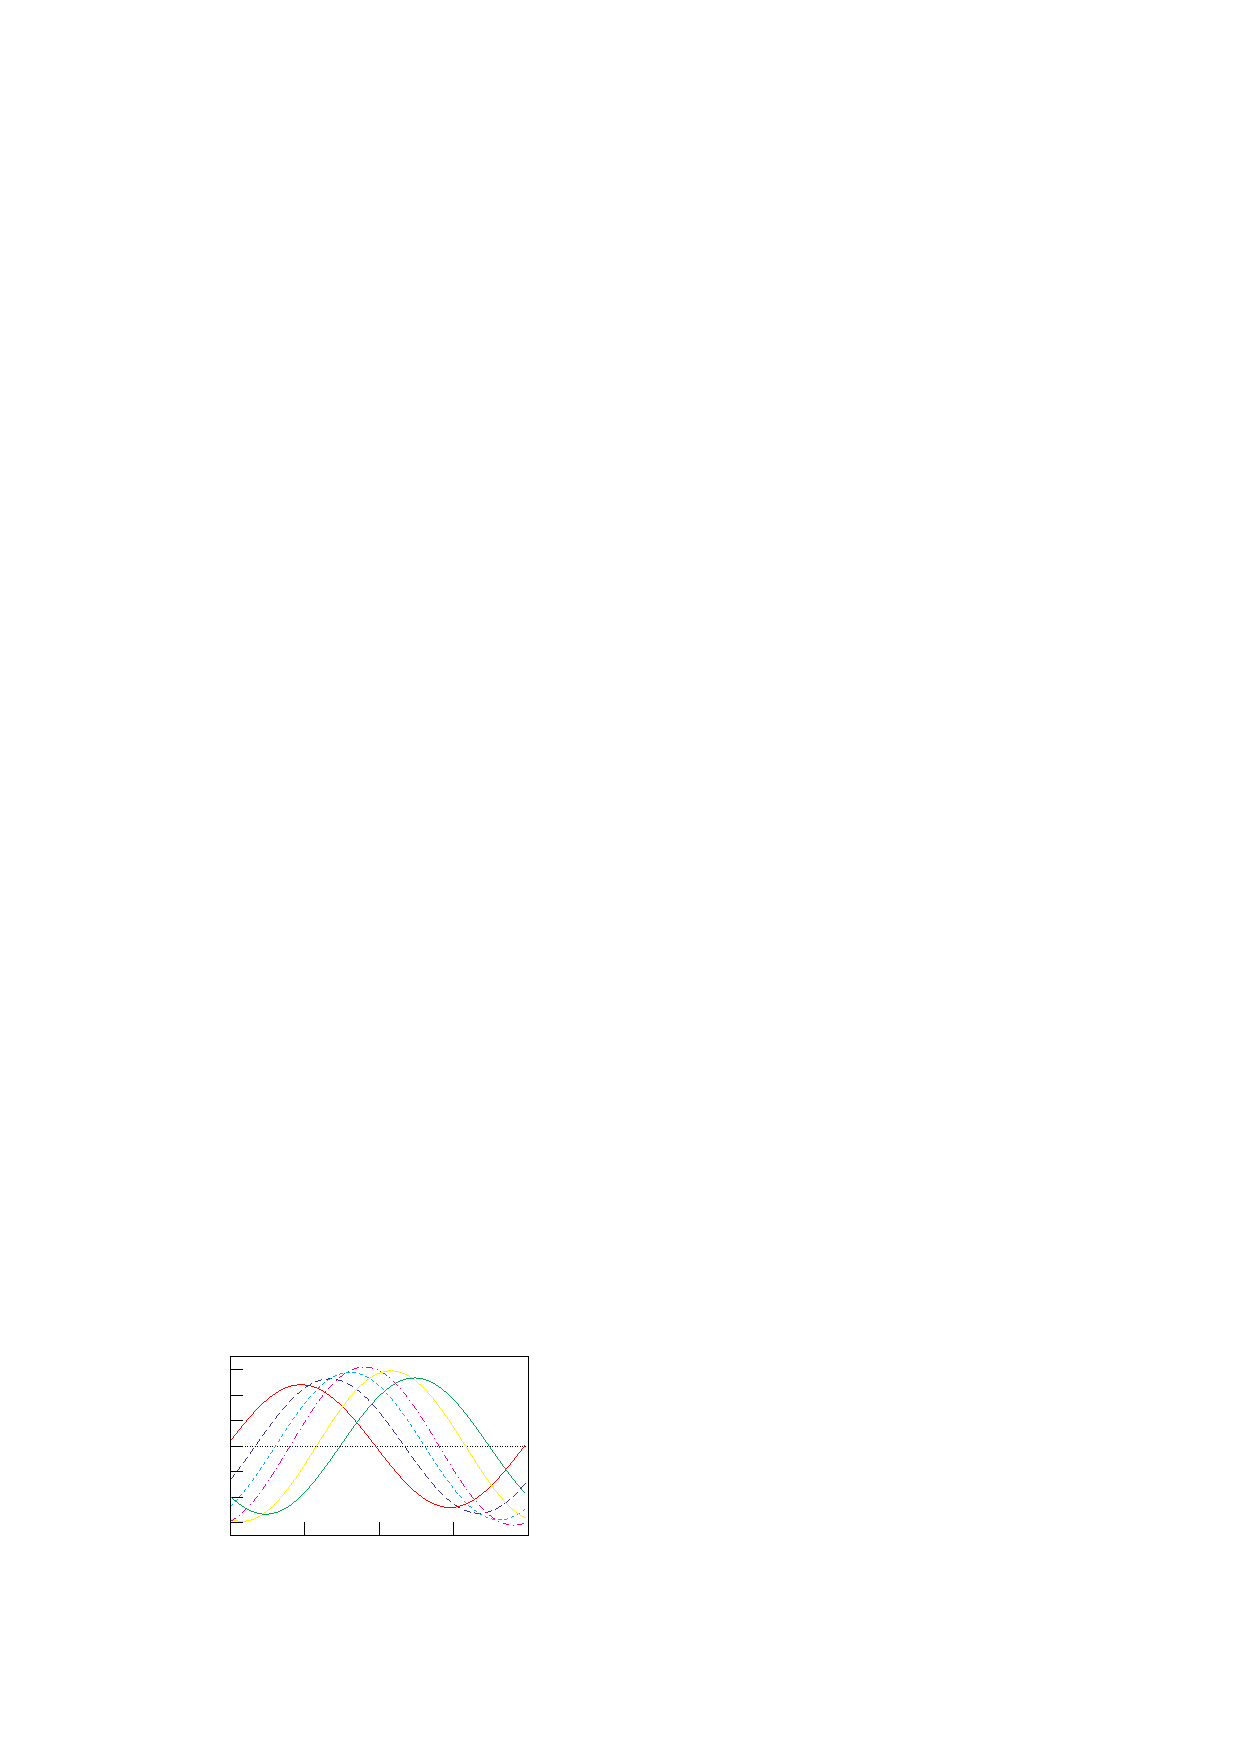
\includegraphics{Images/epslatex/Mel_ext_2}%
\end{picture}%
\begingroup
\setlength{\unitlength}{0.0200bp}%
\begin{picture}(9900,6480)(0,0)%
\put(1650,5624){\makebox(0,0)[r]{\strut{} 3}}%
\put(1650,5013){\makebox(0,0)[r]{\strut{} 2}}%
\put(1650,4401){\makebox(0,0)[r]{\strut{} 1}}%
\put(1650,3790){\makebox(0,0)[r]{\strut{} 0}}%
\put(1650,3179){\makebox(0,0)[r]{\strut{}-1}}%
\put(1650,2567){\makebox(0,0)[r]{\strut{}-2}}%
\put(1650,1956){\makebox(0,0)[r]{\strut{}-3}}%
\put(9075,1100){\makebox(0,0){\strut{}$2\pi$}}%
\put(7287,1100){\makebox(0,0){\strut{}$3\pi\slash{2}$}}%
\put(5500,1100){\makebox(0,0){\strut{}$\pi$}}%
\put(3713,1100){\makebox(0,0){\strut{}${\pi}\slash{2}$}}%
\put(1925,1100){\makebox(0,0){\strut{}0}}%
\put(550,3790){\rotatebox{90}{\makebox(0,0){\strut{}$\mathcal{M}^{\left(1\right)}_{h}\left(\psi_{0}\right)$}}}%
\put(5500,275){\makebox(0,0){\strut{}$\psi_0$}}%
\end{picture}%
\endgroup
\endinput
 \label{fig:Mel_ext_2} }
\end{center}
\caption[Mel'nikov integrals for extensible rods in a magnetic field]{Mel'nikov integrals evaluate at homoclinic energy level where $B=1$, subfigure~\ref{fig:Mel_ext_1} displays a functions at a differing degrees of extensibility, as $(1\slash{J}-1\slash{K})$ ranges from $0.1$ to $0.2$ in increments of $0.02$. In subfigure~\ref{fig:Mel_ext_1} the Casimir $C_{2}$ varies from $1$ up to $2$ in increments of $0.2$.}
\label{fig:Mel_ext}
\end{figure}
% 
\par
By Mel'nikov's theorem~\ref{thm:melnikov} and its corollary~\ref{cor:melnikov} the system is no longer completely integrable if extensible. The transversal intersection of the unstable and unstable manifolds lead to Smale horseshoes on the Poincar\'e section of the homoclinic energy level. This phenonema is illustrated in figures~\ref{fig:poincare} and~\ref{fig:poincare_all} which clearly show the breakup of integrability into the typical plots, referred to as stochastic layers in~\cite{Guckenheimer83}, associated with the Poincar\'e-Birkhoff theorem. 
%
\begin{figure}[h!tb]
\begin{center}
\subfigure[][$\lambda=0.50$]{ \input{Images/epslatex/poincare_0.50.tex} \label{fig:poincare_0.50} }
\subfigure[][$\lambda=3.50$]{ \input{Images/epslatex/poincare_3.50.tex} \label{fig:poincare_3.50} }
\subfigure[][$\lambda=3.75$]{ \input{Images/epslatex/poincare_3.75.tex} \label{fig:poincare_3.75} }
\subfigure[][$\lambda=4.00$]{ %GNUPLOT: LaTeX picture with Postscript
\begin{picture}(0,0)%
\includegraphics{Images/epslatex/poincare_4.00.eps}%
\end{picture}%
\begingroup
\setlength{\unitlength}{0.0200bp}%
\begin{picture}(9900,6750)(0,0)%
\put(2200,1650){\makebox(0,0)[r]{\strut{}-2.5}}%
\put(2200,2105){\makebox(0,0)[r]{\strut{}-2}}%
\put(2200,2560){\makebox(0,0)[r]{\strut{}-1.5}}%
\put(2200,3015){\makebox(0,0)[r]{\strut{}-1}}%
\put(2200,3470){\makebox(0,0)[r]{\strut{}-0.5}}%
\put(2200,3925){\makebox(0,0)[r]{\strut{} 0}}%
\put(2200,4380){\makebox(0,0)[r]{\strut{} 0.5}}%
\put(2200,4835){\makebox(0,0)[r]{\strut{} 1}}%
\put(2200,5290){\makebox(0,0)[r]{\strut{} 1.5}}%
\put(2200,5745){\makebox(0,0)[r]{\strut{} 2}}%
\put(2200,6200){\makebox(0,0)[r]{\strut{} 2.5}}%
\put(2475,1100){\makebox(0,0){\strut{}-2.5}}%
\put(3795,1100){\makebox(0,0){\strut{}-2}}%
\put(5115,1100){\makebox(0,0){\strut{}-1.5}}%
\put(6435,1100){\makebox(0,0){\strut{}-1}}%
\put(7755,1100){\makebox(0,0){\strut{}-0.5}}%
\put(9075,1100){\makebox(0,0){\strut{} 0}}%
\put(550,3925){\rotatebox{90}{\makebox(0,0){\strut{}$p_{\theta}^{}$}}}%
\put(5775,275){\makebox(0,0){\strut{}$\theta$}}%
\end{picture}%
\endgroup
\endinput
 \label{fig:poincare_4.00} }
\end{center}
\caption[Poincar\'e sections of an extensible rod in a magnetic field on the homoclinic energy level]{\baselineskip=1.0\normalbaselineskip% 
Poincar\'e sections on the homoclinic energy level $h=1.109756$ for varying levels of $\lambda$ at the section determined by $\cos\psi=-0.95$. The Casimirs are $C_{1}=C_{2}=C_{3}=1$, the bending stiffness $B=1$, the torsional stiffness $C=4\slash3$, the applied moment is $M=1.70$ and the compressive stiffnesses are $J=1$, $K=50\slash41$.}
\label{fig:poincare}
\end{figure}
% 
\begin{figure}[h!tb]
\begin{center}
%GNUPLOT: LaTeX picture with Postscript
\begin{picture}(0,0)%
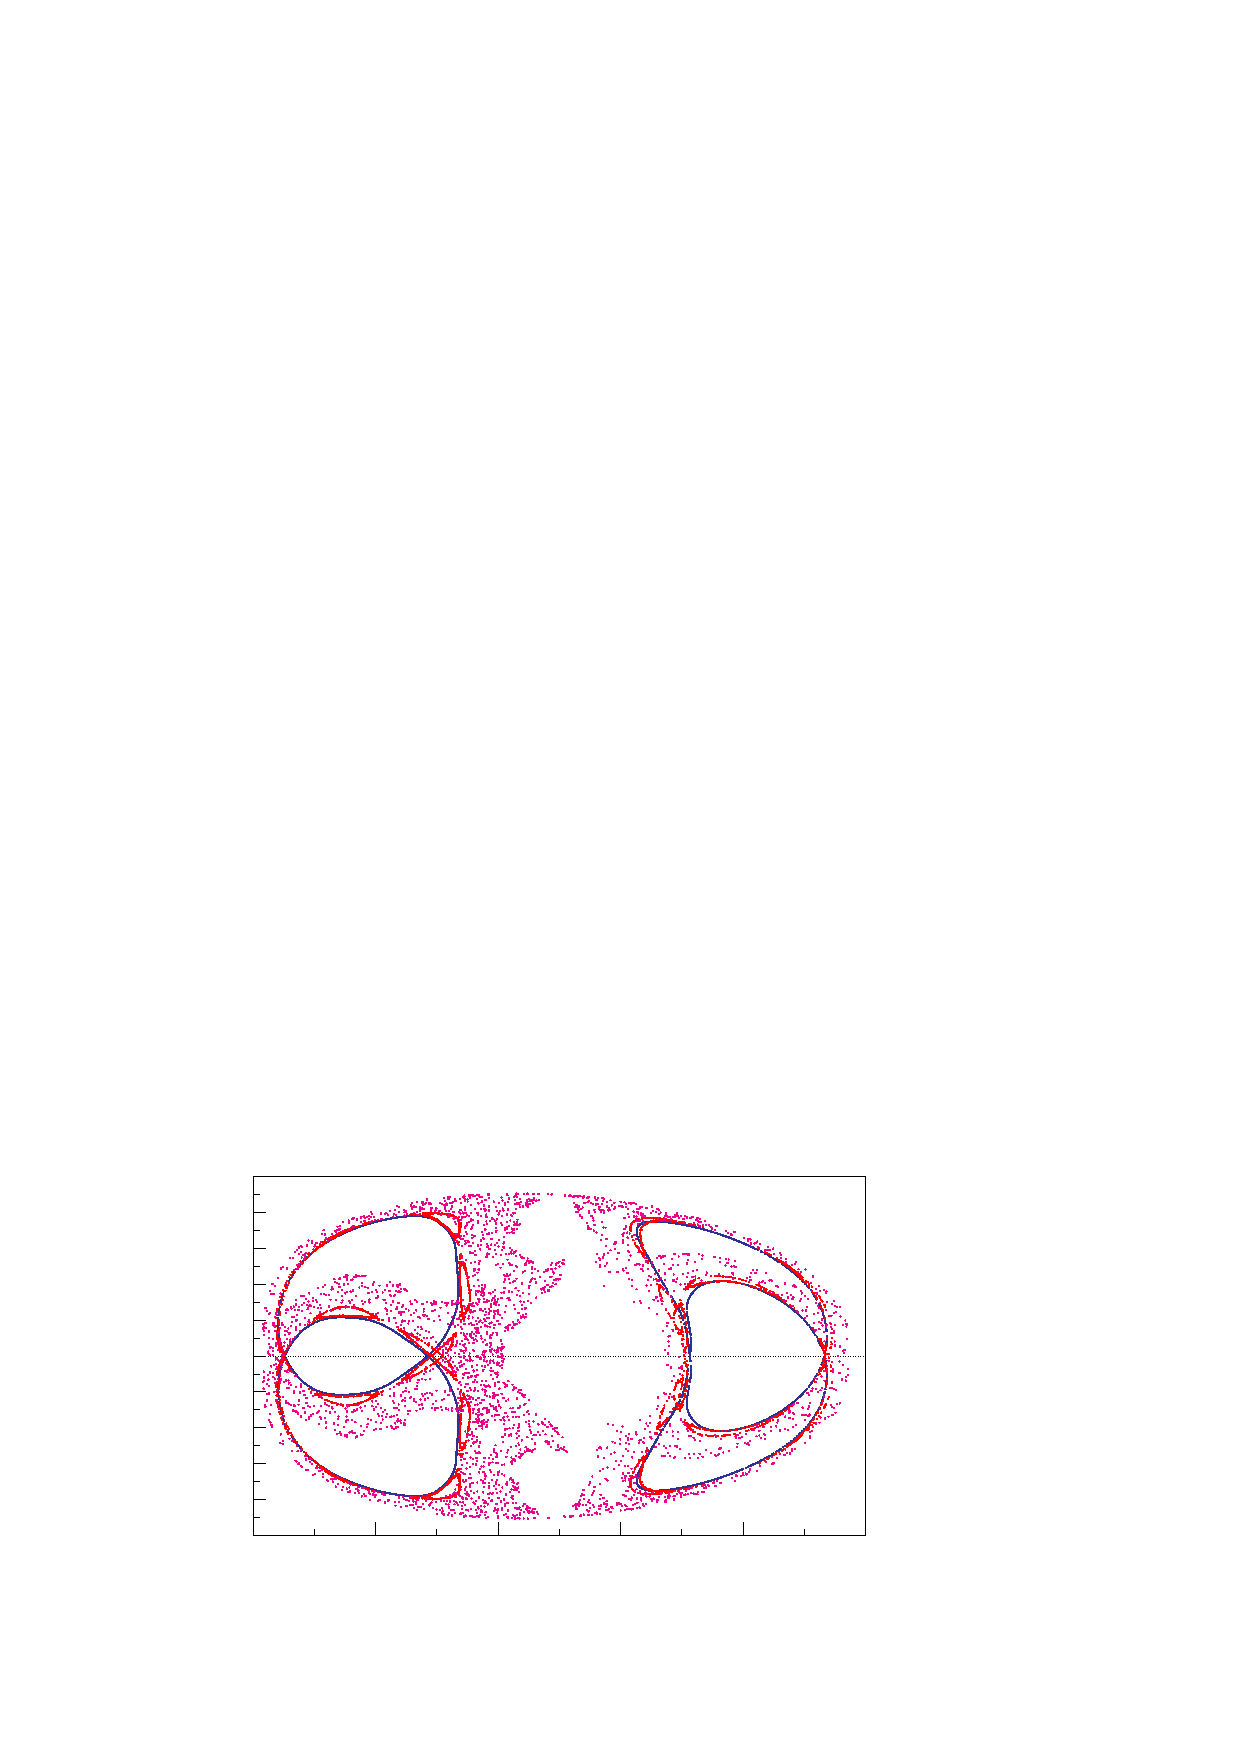
\includegraphics{Images/epslatex/poincare_all}%
\end{picture}%
\begingroup
\setlength{\unitlength}{0.0200bp}%
\begin{picture}(18000,10800)(0,0)%
\put(2200,1650){\makebox(0,0)[r]{\strut{}-2.5}}%
\put(2200,2510){\makebox(0,0)[r]{\strut{}-2}}%
\put(2200,3370){\makebox(0,0)[r]{\strut{}-1.5}}%
\put(2200,4230){\makebox(0,0)[r]{\strut{}-1}}%
\put(2200,5090){\makebox(0,0)[r]{\strut{}-0.5}}%
\put(2200,5950){\makebox(0,0)[r]{\strut{} 0}}%
\put(2200,6810){\makebox(0,0)[r]{\strut{} 0.5}}%
\put(2200,7670){\makebox(0,0)[r]{\strut{} 1}}%
\put(2200,8530){\makebox(0,0)[r]{\strut{} 1.5}}%
\put(2200,9390){\makebox(0,0)[r]{\strut{} 2}}%
\put(2200,10250){\makebox(0,0)[r]{\strut{} 2.5}}%
\put(2475,1100){\makebox(0,0){\strut{}-2.5}}%
\put(5415,1100){\makebox(0,0){\strut{}-2}}%
\put(8355,1100){\makebox(0,0){\strut{}-1.5}}%
\put(11295,1100){\makebox(0,0){\strut{}-1}}%
\put(14235,1100){\makebox(0,0){\strut{}-0.5}}%
\put(17175,1100){\makebox(0,0){\strut{} 0}}%
\put(550,5950){\rotatebox{90}{\makebox(0,0){\strut{}$p_{\theta}^{}$}}}%
\put(9825,275){\makebox(0,0){\strut{}$\theta$}}%
\end{picture}%
\endgroup
\endinput

\end{center}
\caption[Poincar\'e sections of an extensible rod in a magnetic field on the homoclinic energy level at various $\lambda$]{\baselineskip=1.0\normalbaselineskip% 
Poincar\'e sections on the homoclinic energy level $h=1.109756$ for varying levels of $\lambda$ at the section determined by $\cos\psi=-0.95$ showing the collapse of the integrable structure. The Casimirs are $C_{1}=C_{2}=C_{3}=1$, the bending stiffness $B=1$, the torsional stiffness $C=4\slash3$, the applied moment is $M=1.70$ and the compressive stiffnesses are $J=1$, $K=50\slash41$. The projection at $\lambda=3.50$ is in dark blue, $\lambda=3.75$ in red and $\lambda=4.00$ in purple.}
\label{fig:poincare_all} 
\end{figure}
%
%
% note line 490, 603, 388, 409
%
\chapter{Homoclinic Bifurcation of a Rod in a Magnetic Field} \label{chap:bifurcation}
%
\par % Intro
Having derived homoclinics in the unperturbed integrable case and proved the existence of multimodal homoclinics in perturbed nonintegrable cases, in this chapter homoclinic solutions shall be constructed and their bifurcation structure investigated for both primary and multimodal configurations.
% 
\par % overview of technical detail
The computation of homoclinic solutions requires that the arclength be truncated from the infinite domain $s \in \left(-\infty,+\infty\right)$ to the interval $s \in \left[0,\mathcal{T}\right]$. The computation of homoclinics then becomes a boundary value problem where the left-hand side conditions are placed in the unstable mainfold of the trivial equilibrium and the right-hand side conditions satisfy a reversibility. By using the Newton-Raphson method to solve a variational equation with respect to a set of shooting parameters at each iteration, the boundary value problem is then solved using a shooting method. Due to the magnetic effects the system investigated in this chapter is nongeneric as the trivial solution is a periodic orbit, so specific details of the computation and continuation of homoclinic particular to this system are explained. For further details on the computation and continuation of homoclinic solutions in a more general case see appendix~\S\ref{chap:numerics}. 
%
\par % Introduce Euler parameters
In order to increase the computational efficiency the four Euler parameters $q~=~\left(q_{1},q_{2},q_{3},q_{4}\right)$ are used to reduce the dimension of the system. The rotation matrix~\eqref{eq:frame} is then given by
%
\begin{align}
R & = 
\left(
\begin{array}{ccc}
q_{1}^{2} - q_{2}^{2} - q_{3}^{2} + q_{4}^{2} & 2\left(q_{1}^{}q_{2}^{} - q_{3}^{}q_{4}^{}\right) & 2\left( q_{1}^{}q_{3}^{} + q_{2}^{}q_{4}^{} \right) \\
2\left(q_{1}^{}q_{2}^{} + q_{3}^{}q_{4}^{} \right) & q_{2}^{2} + q_{4}^{2} - q_{1}^{2} - q_{3}^{2} & 2\left(q_{2}^{}q_{3}^{} - q_{1}^{}q_{4}^{} \right) \\
2\left(q_{1}^{}q_{3}^{} - q_{2}^{}q_{4}^{} \right) & 2\left(q_{1}^{}q_{4}^{} - q_{2}^{}q_{3}^{} \right) & q_{3}^{2} + q_{4}^{2} - q_{1}^{2} - q_{2}^{2}
\end{array}
\right). \label{eq:ep}
\end{align}
%
The four Euler parameters give a double covering of the set of rotations subject to the constraint 
%
\begin{align}
{q}\cdot{q} = q_{1}^{2} + q_{2}^{2} + q_{3}^{4} + q_{4}^{2} & = 1. \label{eq:ep_Casimir}
\end{align}
%
The Euler parameters are robust in that unlike the Euler angles there is no polar singularity. They are a projection of the phase space onto the surface of a four-dimensional unit sphere. For more details on the Euler parameters and their relation to the Euler angles see appendix~\S\ref{chap:parameterisation}.
% 
\par % e_{3}
From~\eqref{eq:ep} the triple $\mathsf{e}_{1}$ becomes a function of the Euler parameters. 
%
\begin{align}
\mathsf{e}_{3}\left(q\right) & = \left( \begin{array}{c}
2 \left( q_{1}^{}q_{3}^{} + q_{2}^{}q_{4}^{} \right) \\
2 \left( q_{2}^{}q_{3}^{} - q_{1}^{}q_{4}^{} \right) \\
q_{3}^{2} + q_{4}^{2} - q_{1}^{2} - q_{2}^{2}
\end{array}\right).
\label{eq:e3_ep}
\end{align}
% 
\par % Strains
From~\eqref{eq:curvatures} the strains can be written as
%
\begin{align}
u_{i} & = \frac{ 2 \, B_{i} \, q \cdot q^{\prime}}{ q \cdot q } \quad \mbox{for} \quad i=1,2,3 \label{eq:euler_strains}
\end{align}
%
where the ${B}_{i}$ are four-by-four skew-symmetric matrices satisfying the relationships
%
\begin{align}
B_{1}q & = \left( q_{4}, q_{3}, -q_{2}, -q_{1} \right), \nonumber \\
B_{2}q & = \left( -q_{3}, q_{4}, q_{1}, -q_{2} \right), \nonumber \\
B_{3}q & = \left( q_{2}, -q_{1}, q_{4}, -q_{3} \right). \nonumber
\end{align}
%
The four vectors $\left\{ q, B_{1}q, B_{2}q, B_{3}q \right\}$ form an orthonormal basis in $\mathbb{R}^{4}$. Thus~\eqref{eq:euler_strains} subject to~\eqref{eq:ep_Casimir} can be inverted and solved for the derivatives of the Euler parameters as
%
\begin{subequations}
\label{eq:ep_evolution}
\begin{align}
q_{1}^{\prime} & = \left( u_{1}q_{4} - u_{2}q_{3} + u_{3}q_{2} \right)\slash{2},\\
q_{2}^{\prime} & = \left( u_{1}q_{3} + u_{2}q_{4} - u_{3}q_{1} \right)\slash{2},\\
q_{3}^{\prime} & = \left(-u_{1}q_{2} + u_{2}q_{1} + u_{3}q_{4} \right)\slash{2},\\
q_{4}^{\prime} & = \left(-u_{1}q_{1} - u_{2}q_{2} - u_{3}q_{3} \right)\slash{2}.
\end{align}
\end{subequations}
% 
Thus, the formulation of the governing equations based on the force and moment balance equations~\eqref{eq:magnetic_moment},~\eqref{eq:magnetic_force} with the constraint~\eqref{eq:ep_evolution} and body force~\eqref{eq:e3_ep} is a dynamical system of the form
%
\begin{align}
\boldsymbol{x}^{\prime} & = f \left(\boldsymbol{x}, \mu \right), \quad \boldsymbol{x} \in \mathbb{R}^{10} \quad \mbox{and} \quad \mu \in \mathbb{R}^{p}, \label{eq:equation}
\end{align}
%
where $p$ is the number of independent nondimensional parameters under consideration. 
%
\par % Boundary Conditions and nondimensionisation
It is assumed that a moment, $M$, and tension, $T$, are applied axially at $s=\pm\infty$. For simplicity let the constitutive relations take the form
%
\begin{equation}
u_{1} = m_{1}\slash B, \quad u_{2} = m_{2} \slash B, \quad u_{3} = m_{3}\slash C \quad \mbox{and} \quad v_{3} = 1 + n_{3}\slash J.
\end{equation}
% 
The system is then nondimensionalised by
%
\begin{equation}
\begin{array}{c}
t = \left(M\slash B\right) s, \quad x_{1} = n_{1}\slash{T},\quad x_{2} = n_{2}\slash{T},\quad x_{3} = \left(n_{3}-T\right)\slash{T},\\
x_{4} = m_{1}\slash{M},\quad x_{5} = m_{2}\slash{M},\quad x_{6} = \left(m_{3}-M\right)\slash{M},\\
x_{7}=q_{1}, \quad x_{8}=q_{2}, \quad x_{9}=q_{3}, \quad x_{10}=q_{4}. \\
\end{array}
\end{equation}
%
The nondimensional parameters for an extensible rod are then given by
%
\begin{equation}
m = \frac{M}{\sqrt{BT}}, \quad \bar\lambda = \frac{\lambda B}{M}, \quad \nu = \frac{B}{C}-1 \quad \mbox{and} \quad \epsilon = \frac{T}{J}.
\end{equation}
%
The nondimensional parameters are the same as those in~\eqref{eq:nondim} with the additional parameter $\bar\lambda$ as the unified magnetic body force parameter. The bar notation is suppressed from this point onwards. Thus, explicitly the governing equations are
%
\begin{subequations}
\label{eq:ge_full}
\begin{align}
x_{1}^{\prime}  & = \left( 1 + \nu \right)x_{2}x_{6} - x_{3}x_{5} + 2 \lambda\left(1+\epsilon x_{3}\right)\left( x_{7}x_{10} + x_{8}x_{9}\right), \\
x_{2}^{\prime}  & = x_{3}x_{4} - \left(1+\nu\right)x_{1}x_{6} - 2\lambda\left(1+\epsilon x_{3}\right)\left(x_{7}x_{9}-x_{8}x_{10}\right), \\
x_{3}^{\prime}  & = x_{1}x_{5} - x_{2}x_{4}, \\
x_{4}^{\prime}  & = \nu x_{5}x_{6} + x_{2}\left( 1 + \epsilon x_{3} \right) \slash m^{2}, \\
x_{5}^{\prime}  & =-\nu x_{4}x_{6} - x_{1}\left( 1 + \epsilon x_{3} \right) \slash m^{2}, \\
x_{6}^{\prime}  & = 0, \\
x_{7}^{\prime}  & = \left( x_{4}x_{10} - x_{5}x_{9} + \left(1+\nu\right)x_{6}x_{8} \right)\slash{2}, \\
x_{8}^{\prime}  & = \left( x_{4}x_{9} + x_{5}x_{10} - \left(1+\nu\right)x_{6}x_{7} \right)\slash{2},\\
x_{9}^{\prime}  & = \left(-x_{4}x_{8} + x_{5}x_{7} + \left(1+\nu\right)x_{6}x_{10} \right)\slash{2},\\
x_{10}^{\prime} & = \left(-x_{4}x_{7} - x_{5}x_{8} - \left(1+\nu\right)x_{6}x_{9} \right)\slash{2}.
\end{align}
\end{subequations}
%
It is a straight-forward exercise to check that the Casimirs~\eqref{eq:magnetic_casimirs}, 
%
\begin{subequations}
\label{eq:nondim_casimirs}
\begin{align}
\dfrac{1}{2} x_{1}^{2} + \dfrac{1}{2} x_{2}^{2} + \dfrac{1}{2} x_{3}^{2} +  2 \lambda x_{4} \left( x_{7}x_{9} + x_{8}x_{10} \right) + 2 \lambda x_{5} \left( x_{8}x_{9} - x_{7}x_{10} \right) \nonumber \\
\hspace{1.0cm} + \lambda x_{6} \left( x_{10}^{2}+x_{9}^{2}-x_{8}^{2}-x_{7}^{2} \right) & = \dfrac{1}{2} + \lambda, \label{eq:nondim_casimir_1} \\
x_{1} \left(  x_{7}x_{9} + x_{8}x_{10} \right) + x_{2} \left( x_{8}x_{9} - x_{7}x_{10} \right) + x_{3} \left( x_{10}^{2}+x_{9}^{2}-x_{8}^{2}-x_{7}^{2} \right) & =1, \label{eq:nondim_casimir_2} \\
\left( x_{7}x_{9} + x_{8}x_{10}\right)^{2} + \left( x_{8}x_{9} - x_{7}x_{10}\right)^{2} + \left( x_{10}^{2}+x_{9}^{2}-x_{8}^{2}-x_{7}^{2}\right)^{2} & = 1, \label{eq:nondim_casimir_3}
\end{align}
\end{subequations}
%
first integrals~\eqref{eq:magnetic_integrals} 
%
\begin{subequations}
\label{eq:nondim_integrals}
\begin{align}
x_{6} & = 1, \label{eq:nondim_integral_1} \\
x_{1} x_{4} + x_{2} x_{5} + x_{3} x_{6} +  \lambda \left( x_{10}^{2}+x_{9}^{2}-x_{8}^{2}-x_{7}^{2} \right) & = 1 + \lambda \label{eq:nondim_integral_2}
\end{align}
\end{subequations}
%
and constraint~\eqref{eq:ep_Casimir} 
%
\begin{align}
 x_{7}^{2} + x_{8}^{2} + x_{9}^{2} + x_{10}^{2} & = 1 \label{eq:nondim_constraint}
\end{align}
%
are all conserved quantities.
%
\par % Periodicity
The periodic orbit, with period given by $\tau = 2\pi\slash\left(1+\nu\right)$ of the system~\eqref{eq:ge_full}, which satisfys the boundary conditions, constraint and the correct orientation of the director frame is given by
%
\begin{align}
\boldsymbol{x}_{0}\left(s\right) & = \left( 0, 0, 1, 0, 0, 1, 0, 0, \sin \left( s\left(1+\nu\right)\slash 2\right), \cos\left( s\left(1+\nu\right) \slash 2\right) \right). \label{eq:trivial}
\end{align}
%
Monodromy matrices are used to study the stability of periodic orbits. From  
% 
\begin{equation}
\dfrac{\partial }{\partial s} \left[ \dfrac{\partial \boldsymbol{x}_{0}}{\partial \boldsymbol{x}} \right] = \dfrac{\partial }{\partial \boldsymbol{x}} \left[ \dfrac{\partial \boldsymbol{x}_{0}}{\partial s} \right] = \dfrac{\partial }{\partial s} f\left(\boldsymbol{x}_{0},\mu\right) = \left. \left[ \dfrac{\partial f}{\partial \boldsymbol{x}} \right] \right|_{\boldsymbol{x}=\boldsymbol{x}_{0}} \left[ \dfrac{\partial \boldsymbol{x}_{0}}{\partial \boldsymbol{x}} \right] \nonumber 
\end{equation}
% 
then the monodromy matrix $M\left(s\right)$ is determined by the solution to the $10$-dimensional system of linear ordinary differential equations given by
% 
\begin{equation}
M^{\prime} = \left[ \dfrac{\partial f}{\partial \boldsymbol{x}} \right]  M \quad \mbox{with} \quad M\left(0\right) = \mathbb{I}_{10}.
\end{equation}
% 
The period $\tau$ mapping the image of the periodic orbit~\eqref{eq:trivial} is a fixed point $\boldsymbol{p}$. Furthermore, the monodromy matrix is the local linearisation of the mapping evaluated at the fixed point. This essentially means that the monodromy matrix determines the local dynamics of the system at the fixed point which represents the periodic orbit. It can be shown that the monodromy matrix is isomorphic to a Poincar\'e map (see~\cite[\S{7}]{Seydel94} for further details).
%
\par % Floquet
When integrated over the period $\tau$, the monodromy matrix $M\left(\tau\right)$ decouples into two matrices; a four-by-four matrix containing the three Casimirs~\eqref{eq:nondim_casimirs} and the constraint~\eqref{eq:nondim_constraint} of the Euler parameters and a six-by-six matrix containing the nontrivial dynamics. Note that the trivial dynamics yield a trivial Floquet multiplier $\mu^{t}=1$ with algebraic and geometric multiplicity equal to four. The nontrivial monodromy matrix has a pair of complex conjugate unstable Floquet multipliers, $\mu^{u}$, a pair of complex conjugate stable Floquet multipliers, $\mu^{s}$, and a pair of purely imaginary conjugates on the unit circle, $\mu^{c}$. The local stable, centre and unstable manifolds are thus all two dimensional. 
%
\par % Lyapunov
The Lyapunov Centre Theorem states that there exists an analytic one-parameter family of symmetric periodic orbits of the vector field about a fixed point, $\boldsymbol{p}$, which are all contained in a two dimensional local smooth invariant manifold. The family of periodic orbits are straight twisted rods parameterised by Poisson's ratio, $\nu$ and the fixed point corresponds to a straight untwisted rod.
%
\par % Codimension - general
Generically homoclinic connections between fixed points in reversible saddle-focus systems are a codimension-one phenomena, however, if the system is Hamiltonian or reversible homoclinics are a codimension-zero phenomena~\cite{Devaney78}. The explanation is as follows: the intersection of the $2n$-dimensional stable and unstable manifolds at the $2n$-dimensional symmetric section will be a codimension-one phenomena, but when the system is Hamiltonian the intersection occurs along an energy level defined by the Hamiltonian function and is thus codimension-zero. 
%
\par % Codimension - specific
Homoclinic connections between periodic orbits will be a codimension-two phenomena~\cite{Champneys97d}. This is because for homoclinic to periodic orbits two simultaneous codimension-one phenomena occur; firstly a connection between fixed points $\boldsymbol{p}$ of a Poincar\'e return map of the periodic orbit and secondly a homoclinic orbit from those fixed points. For a general Hamiltonian system homoclinic the homoclinics are a codimension-one phenomena since the connections between fixed points of the Poincar\'e map are a codimension-zero phenomena. However, in this instance the form of the periodic orbit is known and is independent of the principle continuation parameter. Thus two independent codimension-zero phenomena occur simultaneously: the homoclinic orbit in a Hamiltonian system, determined by the bifurcation parameter, $\lambda$, and the fixed points of the Poincar\'e map, determined by the parameter on the centre manifold, $\nu$.
% 
\par % Spectrum
The Floquet multipliers can only be computed numerically using the integrator $\texttt{dop853.f}$ and the robust eigenvalue/eigenvector subroutine $\texttt{f02agf.f}$\footnote{This is the standard eigenvalue/eigenvector subroutine used throughout this thesis. The subroutine calculates all the eigenvalues and eigenvectors of a real unsymmetric matrix. It is available from \texttt{www.nag.co.uk}. The subroutine was choosen as it is used within the continuation software \textsc{auto}97.}. The spectrum of Floquet multipliers were computed within reasonable bounds and are displayed in figure~\ref{fig:lambda_spectrum}. 
%
\begin{figure}[h!tbp]
\begin{center}
%GNUPLOT: LaTeX picture with Postscript
\begin{picture}(0,0)%
\includegraphics{Images/epslatex/lambda_spectrum}%
\end{picture}%
\begingroup
\setlength{\unitlength}{0.0200bp}%
\begin{picture}(18000,10800)(0,0)%
\put(2200,1650){\makebox(0,0)[r]{\strut{} 1.5}}%
\put(2200,3083){\makebox(0,0)[r]{\strut{} 1.6}}%
\put(2200,4517){\makebox(0,0)[r]{\strut{} 1.7}}%
\put(2200,5950){\makebox(0,0)[r]{\strut{} 1.8}}%
\put(2200,7383){\makebox(0,0)[r]{\strut{} 1.9}}%
\put(2200,8817){\makebox(0,0)[r]{\strut{} 2}}%
\put(2200,10250){\makebox(0,0)[r]{\strut{} 2.1}}%
\put(2475,1100){\makebox(0,0){\strut{} 0}}%
\put(4108,1100){\makebox(0,0){\strut{} 0.02}}%
\put(5742,1100){\makebox(0,0){\strut{} 0.04}}%
\put(7375,1100){\makebox(0,0){\strut{} 0.06}}%
\put(9008,1100){\makebox(0,0){\strut{} 0.08}}%
\put(10642,1100){\makebox(0,0){\strut{} 0.1}}%
\put(12275,1100){\makebox(0,0){\strut{} 0.12}}%
\put(13908,1100){\makebox(0,0){\strut{} 0.14}}%
\put(15542,1100){\makebox(0,0){\strut{} 0.16}}%
\put(17175,1100){\makebox(0,0){\strut{} 0.18}}%
\put(550,5950){\rotatebox{90}{\makebox(0,0){\strut{}$m$}}}%
\put(9825,275){\makebox(0,0){\strut{}$\lambda$}}%
\put(3750,4500){\vector(1,0){2500}}%
\put(5000,3250){\vector(0,1){2500}}%
\put(5000,4500){\circle{1500}}%
\put(5350,4125){\circle{150}}%
\put(5350,4850){\circle{150}}%
\put(6000,5000){\circle{150}}%
\put(6000,4000){\circle{150}}%
\put(5200,5250){\circle{150}}%
\put(5200,3750){\circle{150}}%
\put(5850,8600){\vector(1,0){2500}}%
\put(7100,7350){\vector(0,1){2500}}%
\put(7100,8600){\circle{1500}}%
\put(7825,8950){\circle{150}}%
\put(7825,8250){\circle{150}}%
\put(7600,9200){\circle{150}}%
\put(7600,8000){\circle{150}}%
\put(7300,9350){\circle{150}}%
\put(7300,7850){\circle{150}}%
\end{picture}%
\endgroup
\endinput
%\put(3750,4500){\vector(1,0){2500}}%
%\put(5000,3250){\vector(0,1){2500}}%
%\put(5000,4500){\circle{1500}}%
%\put(5350,4125){\circle{150}}%
%\put(5350,4850){\circle{150}}%
%\put(6000,5000){\circle{150}}%
%\put(6000,4000){\circle{150}}%
%\put(5200,5250){\circle{150}}%
%\put(5200,3750){\circle{150}}%
%\put(5850,8600){\vector(1,0){2500}}%
%\put(7100,7350){\vector(0,1){2500}}%
%\put(7100,8600){\circle{1500}}%
%\put(7825,8950){\circle{150}}%
%\put(7825,8250){\circle{150}}%
%\put(7600,9200){\circle{150}}%
%\put(7600,8000){\circle{150}}%
%\put(7300,9350){\circle{150}}%
%\put(7300,7850){\circle{150}}%
%\end{picture}%
%\endgroup
%\endinput

\end{center}
\caption[Spectrum of the monodromy matrix about the trivial periodic solution]{\baselineskip=1.0\normalbaselineskip%
Spectrum of the monodromy matrix about the trivial periodic solution~\eqref{eq:trivial} when $\nu=1\slash3$. The solid regions correspond elliptic periodic orbits, the dashed lines is the codimension-one curve at which the Floquet multipliers are stationary and reverse direction. Here $\epsilon=0$ (dark blue), $\epsilon=0.05$ (light blue) and $\epsilon=0.1$ (purple).} 
\label{fig:lambda_spectrum}
\end{figure}
%
In figure~\ref{fig:lambda_spectrum} the solid regions correspond to elliptic regions where homoclinic solutions can not exist. The dashed lines corresponds to a codimension-one curve where the pairs of Floquet multipliers are stationary with respect to the principle continuation parameter, that is 
%
\begin{align}
\frac{\partial \mu^{c}}{\partial \lambda} = \frac{\partial \mu^{s}}{\partial \lambda} = \frac{\partial \mu^{u}}{\partial \lambda} & = 0. \nonumber
\end{align}
%
At the cusp points, (where the dashed lines meets the solid regions) there are codimension-two points $\left(\lambda_{c},m_{c}\right)$ at which the pairs of Floquet multipliers satisfy
%
\begin{align}
\frac{\partial \mu^{c}}{\partial \lambda} = \frac{\partial \mu^{s}}{\partial \lambda} = \frac{\partial \mu^{u}}{\partial \lambda} & = 0 \quad \mbox{and} \quad \mu^{c}=\mu^{s}=\mu^{u}. \label{eq:codim_one_curve}
\end{align}
%
Thus, at the codimension-two point all Floquet multipliers lie on the unit circle and have zero derivative, hence the stable and unstable Floquet multipliers graze the unit circle (cf. figures~\ref{fig:bif_diagram} and~\ref{fig:bif_diagram_codim}). If the system was not Hamiltonian the cusp point would be a codimension-three point. Codimension-two points have been computed for a variety of degrees of extensibility and are displayed in table~\ref{tab:codim}.  It shall be shown that the codimension-two point plays a significant role in the bifurcation structure of the rod in a magnetic field.  
%
\begin{table}[h!tbp]
\caption[Codimension-two points $\left(\lambda,m\right)$ for various degrees of extensibility]{\baselineskip=1.0\normalbaselineskip%
Codimension-two points when $\nu=1\slash3$ for a variety of rods with different degrees of extensibility.}
\begin{center}
\begin{tabular}{ccc}
\hline
$\epsilon$ & $m_{c}$ & $\lambda_{c}$ \\ 
0.0  & 1.7398 & 0.10897200 \\
0.01 & 1.7451 & 0.10897395 \\
0.02 & 1.7537 & 0.10790956 \\
0.03 & 1.7622 & 0.10687853 \\
0.04 & 1.7708 & 0.10583647 \\
0.05 & 1.7793 & 0.10482703 \\
0.06 & 1.7877 & 0.10384922 \\
0.07 & 1.7961 & 0.10288132 \\
0.08 & 1.8045 & 0.10192327 \\
0.09 & 1.8129 & 0.10089494 \\
0.10 & 1.8211 & 0.10007644 \\
\hline
\end{tabular}
\label{tab:codim}
\end{center}
\end{table}
%
\section[Computation]{Computation of Homoclinic orbits} \label{sec:computation}
% 
\par % Intro
The computation of solutions over an infinite domain is impossible, thus it is necessary to truncate the domain to a finite interval. In this section the reversibilities of the system shall be exploited to formulate a well-posed boundary value problem for a shooting method which is then solved by forming a variation problem with respect to the shooting parameters. 
%
\par % Shooting boundary conditions: lhs
The reversibilities define a three-dimensional symmetric section, hence three shooting parameters are required in order to satisfy the righthand boundary conditions. Letting the three shooting parameters be $\left(\delta_{1},\delta_{2},\mathcal{T}\right)$, where $\delta_{1} \sim \mathcal{O}\left(1\right)$, $\delta_{2} \in \left(0,2\pi\right)$ and $\mathcal{T} \gg \delta_{1}$ then the lefthand boundary conditions are
%
\begin{align}
\boldsymbol{x}\left(0\right) & = \boldsymbol{p} + \bar{\varepsilon} \delta_{1}\left( \boldsymbol{v}_{1}\sin\delta_{2} + \boldsymbol{v}_{2}\cos\delta_{2} \right). \label{eq:lhs}
\end{align} 
%
The shooting parameter $\delta_{1}$ is a measure of the perturbation away from the equilibrium solution, $\delta_{2}$ ensures that the perturbation remains transverse to the flow, $\boldsymbol{p}$ denotes the fixed point of the return map as 
%
\begin{align}
\boldsymbol{p} & = \boldsymbol{x}_{0}\left(\tau\right) = \left(0,0,1,0,0,1,0,0,0,1\right), \label{eq:phase}
\end{align}
%
$\bar{\varepsilon}$ (small and fixed, here $\bar{\varepsilon}=10^{-5}$) is related to the length of the truncated homoclinic $\mathcal{T}$ and $\boldsymbol{v}_{1}$ and $\boldsymbol{v}_{2}$ are the real and imaginary parts of the eigenvectors that span the unstable (generalised) eigenspace of the monodromy matrix $M\left(\tau\right)$.  For $\nu=1\slash3$, $m=1.90$, $\lambda=0.1$ and $\epsilon=0.1$ the eigenvectors $\boldsymbol{v}_{1}\pm\boldsymbol{v}_{2}i$ corresponding to the unstable Floquet multipliers $\mu^{u}=-1.2861\pm2.5236{i}$ are
%
\begin{subequations}
\begin{align}
\boldsymbol{v}_{1} & = \left(0.5307,  0, 0,  0.2024, -0.02854,  0,  0.1367, -0.3974,  0,  0\right), \nonumber \\
\boldsymbol{v}_{2} & = \left(0,  0.5307,  0,  0.02854,  0.2024,  0,  0.3974,  0.1367,  0,  0\right). \nonumber
\end{align}
\end{subequations}
%
Note that the eigenspace is a subspace of $\mathbb{R}^{10}$ but is homeomorphic to a vector field in $\mathbb{R}^{6}$, the dimension of the reduced phase space as the four zeroes in the vectors correspond to the trivial multiplier $\mu^{t}$.  Effectively the shooting parameters $\delta_{1}$ and $\delta_{2}$ parametrise a solution in the two components of the (local) unstable manifold and $\mathcal{T}$ parametrises `time' along one such trajectory. Due to the truncation, more precisely $\mathcal{T}$ is the `time' spent outside the local unstable manifold. Also note from~\eqref{eq:lhs} that although $\delta_{1}$ and $\mathcal{T}$ are not independent, as an increase in $\delta_{1}$ changes the time spent on the stable and unstable manifold, homoclinic orbits occur continuously for isolated values of the shooting parameters.
%
\par % Shooting boundary conditions: rhs
The righthand boundary conditions are determined by the symmetric section of either reversing involution. The reversibility is given by
%
\begin{equation}
\left( x_{1}, x_{2}, x_{3}, x_{4}, x_{5}, x_{6}, x_{7}, x_{8}, x_{9}, x_{10} \right) \mapsto \left( -x_{1}, -x_{2}, x_{3}, -x_{4}, -x_{5}, x_{6}, x_{7}, x_{8}, -x_{9}, -x_{10} \right) \nonumber  
\end{equation}
%
as $s \mapsto -s$. Note that the fixed point $\boldsymbol{p}$ is invariant under the reversing involutions. The righthand boundary conditions for $R_{1}$ reversibility for the trivial solution~\eqref{eq:trivial} are 
%
\begin{align}
x_{1}\left(\mathcal{T}\right) = x_{4}\left(\mathcal{T}\right) = x_{10}\left(\mathcal{T}\right) - 1 & = 0. \label{eq:rhs}
\end{align}
%
Similarly for the $R_{2}$ reversibility the righthand boundary conditions are given by

\begin{align}
x_{5}\left(\mathcal{T}\right) = x_{5}\left(\mathcal{T}\right) = x_{10}\left(\mathcal{T}\right) - 1 & = 0. \label{eq:rhs1}
\end{align}
% 
Again, recalling that the system, reduced by the Casimirs and constraint defines a canonical six-dimension system. The symmetric section is three-dimensional and the reversibilities are reversibilities in the classical sense.
%
\par % variational equation
Having formulated the boundary value problem as a three-parameter shooting problem, it is necessary to constructs a variational equation from the ten dimensional system~\eqref{eq:ge_full} with respect to the three shooting parameters $\left(\delta_{1},\delta_{2},\mathcal{T}\right)$ which can be solved using the Newton-Raphson method. Thus, at each iteration a forty-dimensional variation equation is solved. Each iteration is not computationally expensive but choosing three good initial guesses is often delicate. When a suitable initial guess is found the shooting method converges quadratically and the conserved quantities are all computed with error of order $\bar{\epsilon}^{2}$ in accordance with the Newton-Raphson scheme. For detail on how the variational equation is formulated and the shooting method is solved, see appendix~\S\ref{sec:shooting}. 
% 
\par % Well posed
Thus, equation~\eqref{eq:equation} subject to boundary conditions~\eqref{eq:lhs} and~\eqref{eq:rhs} forms a well-posed boundary value problem for the construction of a reversible homoclinic about the trivial solution~\eqref{eq:trivial}. Homoclinic solutions are found for all parameter values which are not purely elliptic, thus as stated homoclinics are a codimension-zero phenomena.
%
\par % Shooting data
Table~\ref{tab:rev0} gives some shooting data for a set of primary homoclinic orbits within the hyperbolic region. Tables of shooting values for a selection of multimodal homoclinics are given in tables~\ref{tab:rev1} and~\ref{tab:rev2}. Sample configurations of a primary homoclinic and the forces due to the magnetic effects are displayed in figures~\ref{fig:P1_config} and~\ref{fig:force} and components of a multimodal homoclinic figure~\ref{fig:multimodals}. As seen in~\S\ref{sec:nonintegrable_perturbations} the shooting method can be used to detect a multiplicity of multimodals according to a well-defined set of accumulation and coalescence rules, but while families of bimodals do exist, the shooting method is unable to find all members in a systematic way in the presence of an underlying periodic solution. 
%
\begin{table}[h!t]
\caption[Shooting data for primary homoclinic orbits]{\baselineskip=1.0\normalbaselineskip%
Shooting data for the reversible primary homoclinic orbits when $\nu=1\slash3$, $m=1.90$, $\epsilon=0.1$ and $\lambda=0.1$.}
\begin{center}
\begin{tabular}{ccccc}
\hline 
& & $\delta_{1}$ & $\delta_{2}$ & $\mathcal{T}$ \\ 
$R_{1}$ & $P_{1}$ & 1.058975 & 1.374092 & 60.61385 \\
& $P_{2}$ & 4.200569 & 1.374092 & 60.61385 \\
$R_{2}$ & $P_{3}$ & 0.2069183 & 1.082621 & 58.26191 \\
& $P_{4}$ & 3.348511 & 1.082621 & 58.26191 \\
\hline
\end{tabular}
\label{tab:rev0}
\end{center}
\end{table}
%
\begin{table}[h!t]
\caption[Shooting data for bimodal homoclinic orbits]{\baselineskip=1.0\normalbaselineskip%
Shooting data for some reversible bimodal homoclinic orbits when $\nu=1\slash3$, $m=1.90$, $\epsilon=0.1$ and $\lambda=0.1$.}
\begin{center}
\begin{tabular}{ccccc}
\hline
& & $\delta_{1}$ & $\delta_{2}$ & $\mathcal{T}$ \\ 
$R_{1}$ & $\left(P_{1},n,P_{1}\right)$ & 3.900605 & 2.809424 & 82.48046 \\
& $\left(P_{2},n,P_{1}\right)$ & 0.7590124 & 2.809424 & 82.48046 \\
$R_{2}$ &$\left(P_{3},n,P_{3}\right)$ & 0.8877950 & 1.797026 & 81.18148 \\
& $\left(P_{4},n,P_{3}\right)$ & 4.029388 & 1.797026 & 81.18148 \\
\hline
\end{tabular}
\label{tab:rev1}
\end{center}
\end{table}
% 
\begin{figure}[h!tbp] 
\begin{center}
%GNUPLOT: LaTeX picture with Postscript
\begin{picture}(0,0)%
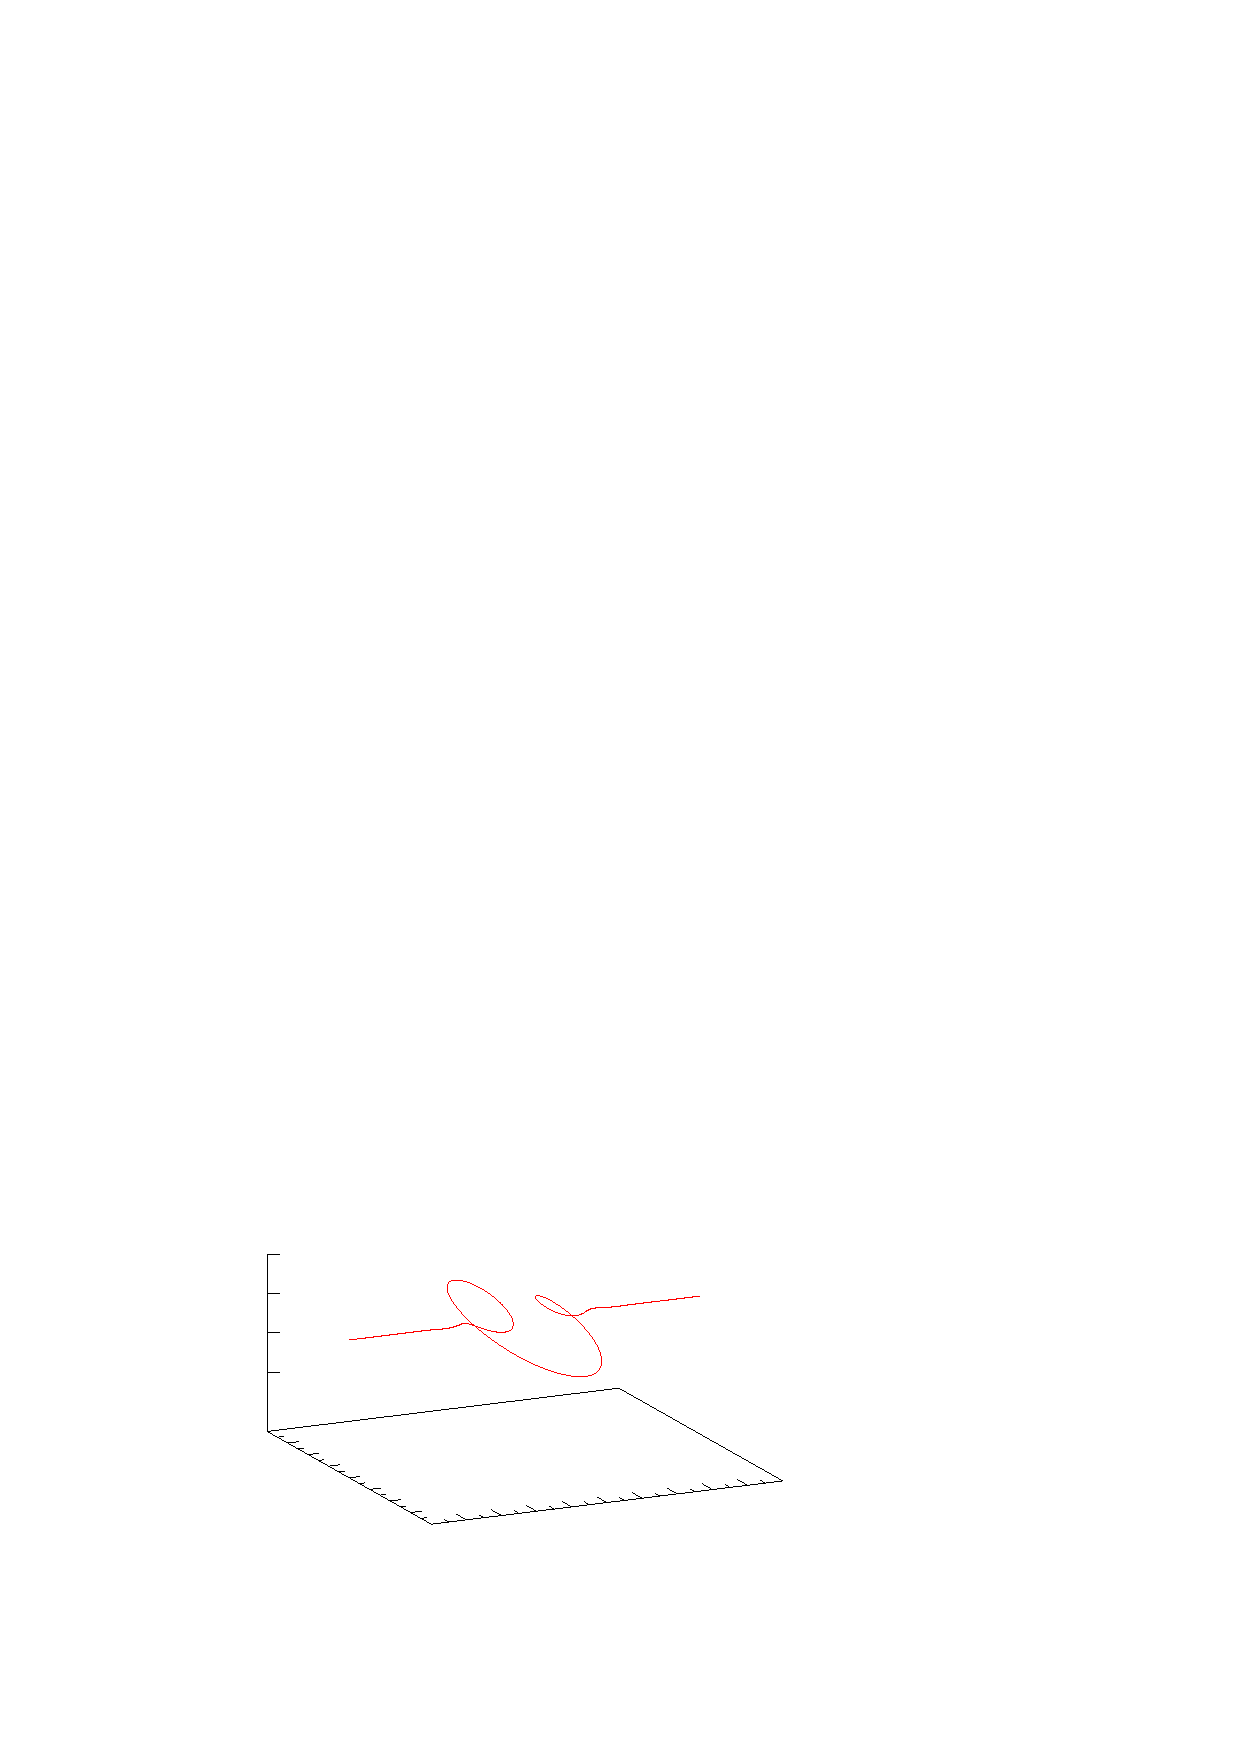
\includegraphics{Images/epslatex/lambda_P1_config}%
\end{picture}%
\begingroup
\setlength{\unitlength}{0.0200bp}%
\begin{picture}(18000,10800)(0,0)%
\put(6968,1667){\makebox(0,0){\strut{} 0}}%
\put(7812,1770){\makebox(0,0){\strut{} 0.2}}%
\put(8657,1874){\makebox(0,0){\strut{} 0.4}}%
\put(9500,1978){\makebox(0,0){\strut{} 0.6}}%
\put(10344,2082){\makebox(0,0){\strut{} 0.8}}%
\put(11188,2186){\makebox(0,0){\strut{} 1}}%
\put(12032,2290){\makebox(0,0){\strut{} 1.2}}%
\put(12876,2393){\makebox(0,0){\strut{} 1.4}}%
\put(13720,2497){\makebox(0,0){\strut{} 1.6}}%
\put(14565,2601){\makebox(0,0){\strut{} 1.8}}%
\put(15409,2705){\makebox(0,0){\strut{} 2}}%
\put(6499,1855){\makebox(0,0)[r]{\strut{}-2}}%
\put(6007,2133){\makebox(0,0)[r]{\strut{}-1.5}}%
\put(5515,2411){\makebox(0,0)[r]{\strut{}-1}}%
\put(5023,2689){\makebox(0,0)[r]{\strut{}-0.5}}%
\put(4531,2968){\makebox(0,0)[r]{\strut{} 0}}%
\put(4039,3246){\makebox(0,0)[r]{\strut{} 0.5}}%
\put(3547,3524){\makebox(0,0)[r]{\strut{} 1}}%
\put(3054,3803){\makebox(0,0)[r]{\strut{} 1.5}}%
\put(2562,4081){\makebox(0,0)[r]{\strut{} 2}}%
\put(2212,5560){\makebox(0,0)[r]{\strut{}-4}}%
\put(2212,6505){\makebox(0,0)[r]{\strut{}-2}}%
\put(2212,7450){\makebox(0,0)[r]{\strut{} 0}}%
\put(2212,8396){\makebox(0,0)[r]{\strut{} 2}}%
\put(2811,9460){\makebox(0,0){\strut{}$y$}}%
\put(11952,1878){\makebox(0,0){\strut{}$z$}}%
\put(2669,2769){\makebox(0,0){\strut{}$x$}}%
\put(2811,9460){\makebox(0,0){\strut{}$y$}}%
\end{picture}%
\endgroup
\endinput
 
\end{center}
\caption[Configuration of primary homoclinic]{\baselineskip=1.0\normalbaselineskip%
Configuration of primary homoclinic $P_{1}$ orbits in table~\ref{tab:rev0}.}
\label{fig:P1_config}
\end{figure} 
% 
\begin{figure}[h!tbp]
\begin{center}
\subfigure{ \input{Images/epslatex/R2_force_1.tex} \label{fig:R2_force_1} }
\subfigure{ %GNUPLOT: LaTeX picture with Postscript
\begin{picture}(0,0)%
\includegraphics{Images/epslatex/R2_force_2}%
\end{picture}%
\begingroup
\setlength{\unitlength}{0.0200bp}%
\begin{picture}(9900,5940)(0,0)%
\put(2475,1650){\makebox(0,0)[r]{\strut{}-0.06}}%
\put(2475,2273){\makebox(0,0)[r]{\strut{}-0.04}}%
\put(2475,2897){\makebox(0,0)[r]{\strut{}-0.02}}%
\put(2475,3520){\makebox(0,0)[r]{\strut{} 0}}%
\put(2475,4143){\makebox(0,0)[r]{\strut{} 0.02}}%
\put(2475,4767){\makebox(0,0)[r]{\strut{} 0.04}}%
\put(2475,5390){\makebox(0,0)[r]{\strut{} 0.06}}%
\put(2750,1100){\makebox(0,0){\strut{} 0}}%
\put(4015,1100){\makebox(0,0){\strut{} 0.2}}%
\put(5280,1100){\makebox(0,0){\strut{} 0.4}}%
\put(6545,1100){\makebox(0,0){\strut{} 0.6}}%
\put(7810,1100){\makebox(0,0){\strut{} 0.8}}%
\put(9075,1100){\makebox(0,0){\strut{} 1}}%
\put(550,3520){\rotatebox{90}{\makebox(0,0){\strut{}$f_{2}$}}}%
\put(5912,275){\makebox(0,0){\strut{}$s$}}%
\end{picture}%
\endgroup
\endinput
 \label{fig:R2_force_2} }
\end{center}
\caption[External force due to magnetic effects]{\baselineskip=1.0\normalbaselineskip%
External force due to magnetic effects for the $P_{1}$ orbits in table~\ref{tab:rev0}. Note that the external forces are reversible.} 
\label{fig:force}
\end{figure}
%
\begin{table}[h!t]
\caption[Shooting data for trimodal homoclinic orbits]{\baselineskip=1.0\normalbaselineskip%
Shooting data for some reversible trimodals homoclinic orbits when $\nu=1\slash3$, $m=1.90$, $\epsilon=0.1$ and $\lambda=0.1$.}
\begin{center}
\begin{tabular}{ccccc}
\hline
& & $\delta_{1}$ & $\delta_{2}$ & $\mathcal{T}$ \\ 
$R_{1}$ & $\left(P_{2},n,P_{2},n,P_{2}\right)$ & 1.449005 & 7.734693 & 101.7462 \\
& $\left(P_{3},n,P_{1},n,P_{4}\right)$ & 4.590598 & 7.734693 & 101.7462 \\
$R_{2}$ & $\left(P_{1},n,P_{4},n,P_{1}\right)$ & 0.5914260 & 6.264897 & 99.38831 \\
& $\left(P_{2},n,P_{3},n,P_{2}\right)$ & 3.7330187 & 6.264897 & 99.38831 \\
\hline
\end{tabular}
\label{tab:rev2}
\end{center}
\end{table}
%
\begin{figure}[h!tbp]
\begin{center}
\subfigure[][$P_{1},n,P_{1}$]{ \input{Images/epslatex/Bimodal_x_1.tex}\label{fig:bimodal_1} }
\subfigure[][$P_{1},n,P_{1}$]{ %GNUPLOT: LaTeX picture with Postscript
\begin{picture}(0,0)%
\includegraphics{Images/epslatex/Bimodal_x_2}%
\end{picture}%
\begingroup
\setlength{\unitlength}{0.0200bp}%
\begin{picture}(9900,6480)(0,0)%
\put(2200,1650){\makebox(0,0)[r]{\strut{}-0.6}}%
\put(2200,2261){\makebox(0,0)[r]{\strut{}-0.4}}%
\put(2200,2873){\makebox(0,0)[r]{\strut{}-0.2}}%
\put(2200,3484){\makebox(0,0)[r]{\strut{} 0}}%
\put(2200,4096){\makebox(0,0)[r]{\strut{} 0.2}}%
\put(2200,4707){\makebox(0,0)[r]{\strut{} 0.4}}%
\put(2200,5319){\makebox(0,0)[r]{\strut{} 0.6}}%
\put(2200,5930){\makebox(0,0)[r]{\strut{} 0.8}}%
\put(2475,1100){\makebox(0,0){\strut{} 0}}%
\put(3795,1100){\makebox(0,0){\strut{} 0.2}}%
\put(5115,1100){\makebox(0,0){\strut{} 0.4}}%
\put(6435,1100){\makebox(0,0){\strut{} 0.6}}%
\put(7755,1100){\makebox(0,0){\strut{} 0.8}}%
\put(9075,1100){\makebox(0,0){\strut{} 1}}%
\put(550,3790){\rotatebox{90}{\makebox(0,0){\strut{}$x_2$}}}%
\put(5775,275){\makebox(0,0){\strut{}$s$}}%
\end{picture}%
\endgroup
\endinput
\label{fig:bimodal_2} }
\subfigure[][$P_{2},n,P_{2},n,P_{2}$]{ \input{Images/epslatex/Trimodal_x_1.tex}\label{fig:trimodal_1} }
\subfigure[][$P_{2},n,P_{2},n,P_{2}$]{ \input{Images/epslatex/Trimodal_x_2.tex}\label{fig:trimodal_2} }
\end{center}
\caption[Force components of a bimodal homoclinic]{\baselineskip=1.0\normalbaselineskip%
Force component $x_{1}$ and $x_{2}$ of bimodal $P_{1},n,P_{2}$ from table~\ref{tab:rev1} shown in~\ref{fig:bimodal_1},~\ref{fig:bimodal_2} and for the trimodal $P_{2},n,P_{2},n,P_{2}$ in table~\ref{tab:rev2}.}
\label{fig:multimodals}
\end{figure} 
%
\par % Multimodals in anisotropic case
Multimodal solutions can be found in the anisotropic system, as shown in figure~\ref{fig:P1_anisotropic_full_quadmodal}, providing numerical evidence that, as in the Kirchhoff rod, anisotropy is an integrability breaking parameter for the linearly elastic, inextensible, unshearable rod in a uniform magnetic field. 
% 
\begin{figure}[h!tbp]
\begin{center}
%GNUPLOT: LaTeX picture with Postscript
\begin{picture}(0,0)%
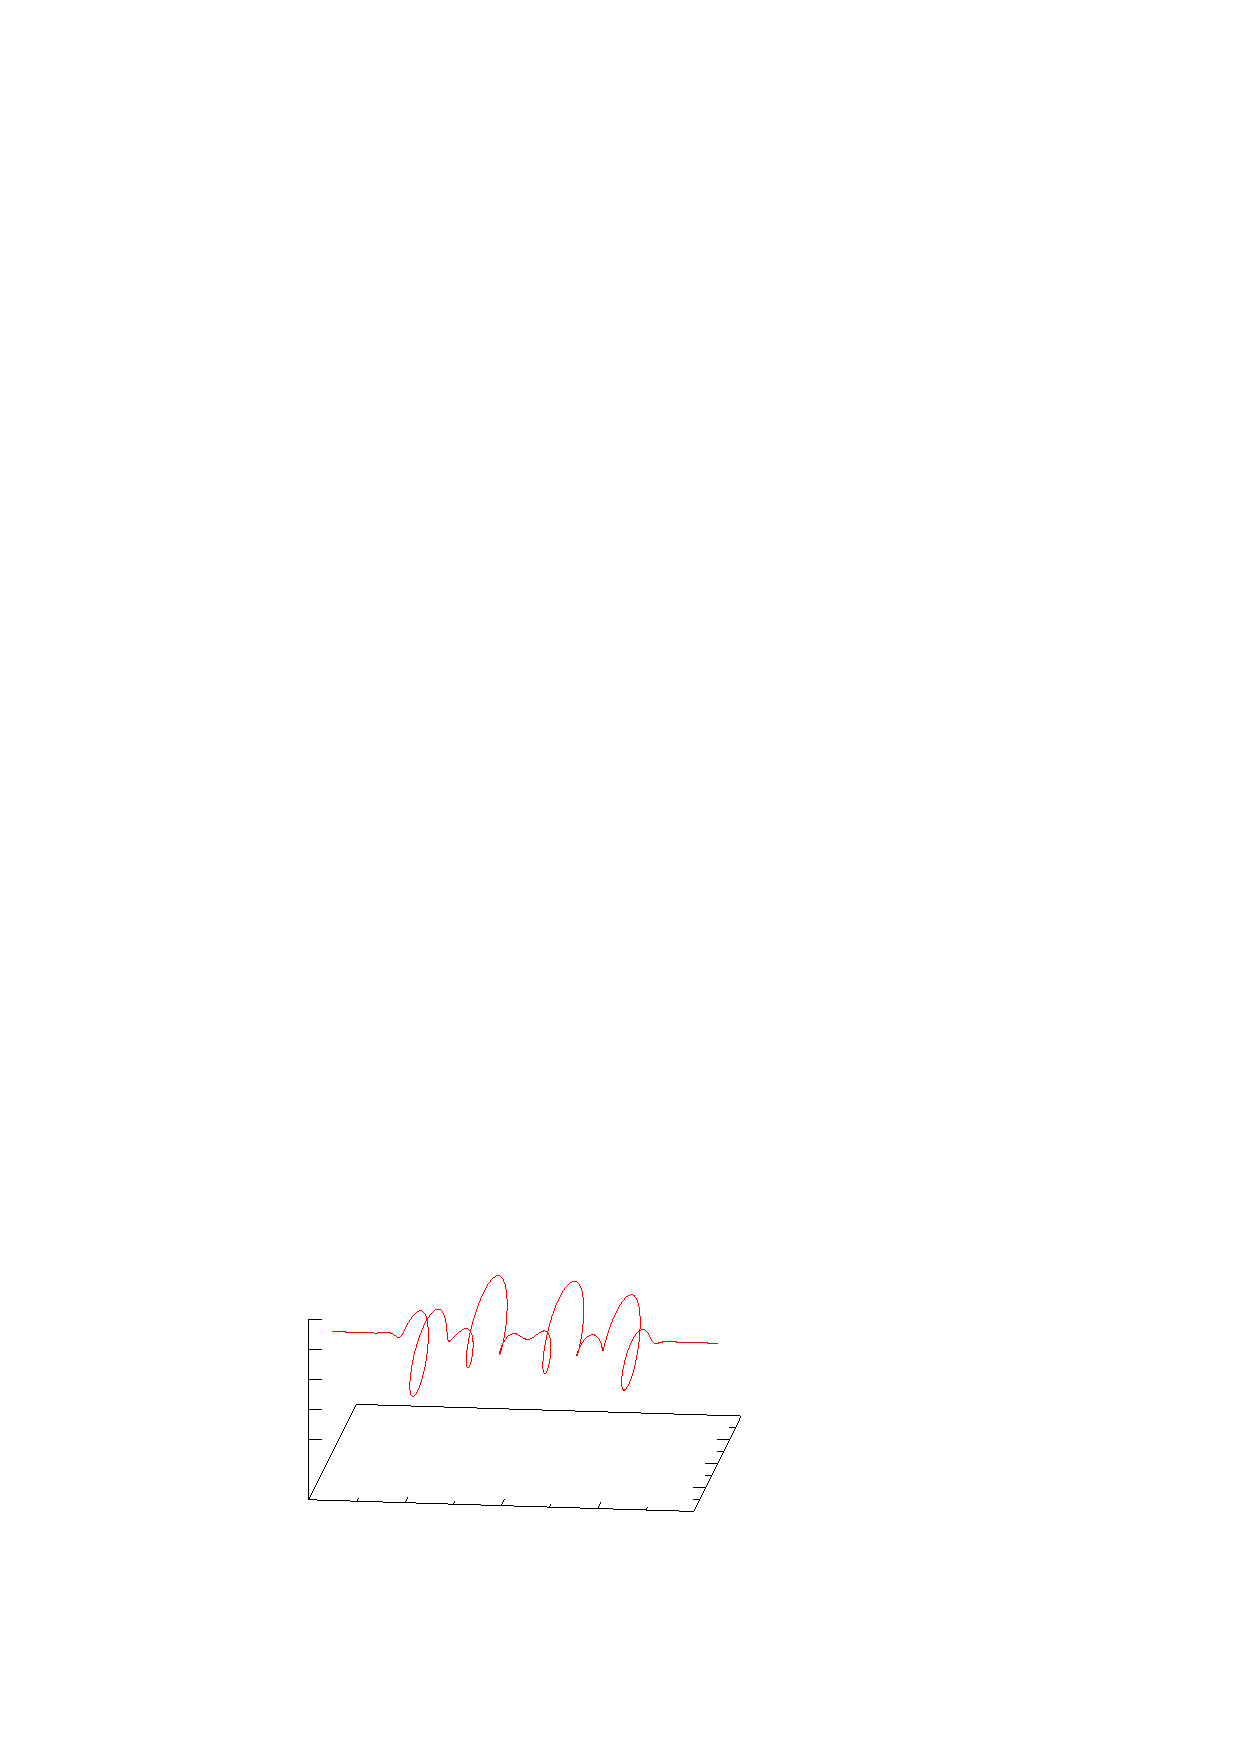
\includegraphics{Images/epslatex/P1_anisotropic_full_quadmodal}%
\end{picture}%
\begingroup
\setlength{\unitlength}{0.0200bp}%
\begin{picture}(18000,10800)(0,0)%
\put(3747,2246){\makebox(0,0){\strut{} 0}}%
\put(6058,2176){\makebox(0,0){\strut{} 0.5}}%
\put(8369,2106){\makebox(0,0){\strut{} 1}}%
\put(10680,2035){\makebox(0,0){\strut{} 1.5}}%
\put(12991,1965){\makebox(0,0){\strut{} 2}}%
\put(13327,2205){\makebox(0,0)[l]{\strut{}-2}}%
\put(13611,2777){\makebox(0,0)[l]{\strut{}-1}}%
\put(13895,3349){\makebox(0,0)[l]{\strut{} 0}}%
\put(14179,3922){\makebox(0,0)[l]{\strut{} 1}}%
\put(14462,4494){\makebox(0,0)[l]{\strut{} 2}}%
\put(3211,3948){\makebox(0,0)[r]{\strut{}-2}}%
\put(3211,4671){\makebox(0,0)[r]{\strut{}-1}}%
\put(3211,5394){\makebox(0,0)[r]{\strut{} 0}}%
\put(3211,6116){\makebox(0,0)[r]{\strut{} 1}}%
\put(3211,6839){\makebox(0,0)[r]{\strut{} 2}}%
\put(3810,7924){\makebox(0,0){\strut{}$x$}}%
\put(8149,1790){\makebox(0,0){\strut{}$z$}}%
\put(15933,3296){\makebox(0,0){\strut{}$y$}}%
\put(3810,7924){\makebox(0,0){\strut{}$x$}}%
\end{picture}%
\endgroup
\endinput
 
\end{center}
\caption[Multimodal configuration in the anisotropic rod in a magnetic field]{\baselineskip=1.0\normalbaselineskip%
A quadmodal with parameters are $\nu={1}\slash{3}$, $\lambda=0.01$, $m=1.70$ and $\rho=0.1$. When $\lambda=0.1$, $m=1.90$ the shooting parameters are given by $\delta_{1} = 5.2433$, $\delta_{2} = 2.1968$ and $\mathcal{T}=85.509$.} 
\label{fig:P1_anisotropic_full_quadmodal}
\end{figure}
% 
% \vspace*{2.0cm}
\section{Continuation} \label{sec:continuation}
%
\par % Projection boundary conditions 
In this section the continuation of configurations is performed using projection boundary conditions~\cite{Beyn90a,Beyn94} exploiting the exponential trichotomies the system possesses~\cite{Klaus03}. The method places solutions in the linearised flow which approximates the tangential flow about a equilibrium configuration. In this system the continuation of periodic-to-periodic homoclinic orbits is simplified~\cite{Champneys97d,Bai96a,Dieci04} by knowing the underlying periodic orbit~\eqref{eq:trivial}. Thus, projecting onto the two-dimensional centre and unstable (generalised) eigenspaces about the phase condition~\eqref{eq:phase} yields the four boundary conditions
%
\begin{subequations}
\label{eq:projection}
\begin{align}
L_{s}\left( \boldsymbol{x}\left(0\right) - \boldsymbol{p} \right) & = \boldsymbol{0}, \label{eq:stable_projection} \\
L_{c}\left( \boldsymbol{x}\left(0\right) - \boldsymbol{p} \right) & = \boldsymbol{0}. \label{eq:centre_projection}
\end{align}
\end{subequations}
% 
Applying the symmetric section boundary conditions, for $R_{1}$ as in~\eqref{eq:rhs}, yields the three boundary conditions
%
\begin{align}
x_{1}\left(1\right) = x_{4}\left(1\right) = x_{10}\left(1\right) & = 0. \label{eq:symmetric}
\end{align}
%
Finally, specifying the three Casimirs~\eqref{eq:nondim_casimirs} and the constraint fixing condition~\eqref{eq:nondim_constraint} gives four boundary conditions
%
\begin{align}
x_{3}\left(0\right) - 1 = x_{6}\left(0\right) - 1 & = x_{9}\left(0\right) = x_{10}\left(0\right) - 1 = 0. \label{eq:integral} 
\end{align}
%
The system~\eqref{eq:ge_full} with boundary conditions~\eqref{eq:projection},~\eqref{eq:symmetric} and~\eqref{eq:integral} is over-determined as there are eleven boundary conditions for a ten dimensional system. Specifically, the projection boundary conditions provide an extra condition, that is there are four boundary conditions determining a flow which can be determined by three (shooting) parameters. Thus, in order to make the problem well-posed the truncation length, $\mathcal{T}$, is allowed to vary along with the principal continuation parameter. %
%
\par % restriction on lambda
It should be noted that while there is no restriction on the sign of $\lambda$, when performing continuation an increase in $\lambda$ acts in the direction of the end load parameter $m$, while decreasing $\lambda$ acts against the load parameter. 
%
\par % Benefits of numerical schemes
Continuation was performed using \textsc{auto97}~\cite{Doedel98}. The continuation software uses Gaussian collocation, which is equivalent to a symplectic Runge-Kutta scheme. Symplectic Runge-Kutta methods exactly conserve the value of any integrals of the system that are quadratic functions of the phase variables~\cite{Channell90}.  Thus, from the Lax pair formulation, presented in \S\ref{sec:lax}, all the  conserved quantities are preserved by the numerical scheme. Note that the Kovalevskaya integral would not be preserved exactly as it is a quartic integral.
%
\par % End deflections
In order to visualise the rod configurations the postprocessed centreline conditions for $\boldsymbol{r}\left(s\right)=\left(x,y,z\right)$, which evolves according to~\eqref{eq:centreline}, are computed from
%
\begin{align}
\boldsymbol{r}\left(0\right) & = \boldsymbol{0}. \label{eq:centreline_ic}
\end{align}
%
Hence the (dimensionless) end-rotation and end-displacement can be calculated while continuing along solution branches of homoclinic orbits for the two parameters $\lambda$ and $\mathcal{T}$. The relative end-deflections represent the true buckling contributions due to the effect of loading by removing the trivial contributions from a unbuckled straight rod. Thus let the relative end-displacement, $\tilde{\mathcal{D}}$ and relative end-rotation $\tilde{\mathcal{R}}$ be given by
%
\begin{subequations}
\begin{align}
\tilde{\mathcal{D}} & = \left(1+\epsilon\right)\mathcal{T} - z\left(1\right), \\
\tilde{\mathcal{R}} & = \frac{\mathcal{R} - \left(1+\nu\right)\mathcal{T}}{2\pi} 
\end{align}
\end{subequations}
%
where 
%
\begin{equation}
\cos \mathcal{R} =\left< \boldsymbol{d}_{1}\left(1\right), \left(1,0,0\right)\right> \quad \mbox{and} \quad \sin \mathcal{R} =\left< \boldsymbol{d}_{1}\left(1\right), \left(0,1,0\right)\right>. \nonumber 
\end{equation}
%
\par
In many respects the end rotation can be thought of as a phase on the sphere defined by $\boldsymbol{r}$. For configurations which have zero first derivative at the end points, such as clamped and homoclinic configurations, the curves on the sphere can be considered to be closed and topological properties such as (open) link, (open) twist and (open) writhe can be related, in a consistent manner, to the phase on the sphere~\cite{Maggs01,Heijden07}. 
% The curves on the sphere are exactly closed on the sphere if the north pole is included, just as the curves in the phase plane illustrated in figure~\ref{fig:super} are closed if the origin is included, cf. remark~\ref{rem:homoclinic}. 
% 
% \begin{figure}[h!tbp]
% \begin{center}
% \input{Images/epslatex/sphere.tex} 
% \end{center}
% \caption[]{\baselineskip=1.0\normalbaselineskip } 
% \label{fig:sphere}
% \end{figure}
% % 
% Then $\mathcal{R}$ is the (open) link, $\left(1+\nu\right)\mathcal{T}$ is the local twist and $\mathcal{R}$ is the writhe of the rod in the celebrated C$\breve{\mathrm{a}}$lug$\breve{\mathrm{a}}$reanu formula~\cite{Langer84}.
%
% \par
% When the end-rotation and end-deflection are zero the rod is a straight rod, hence configurations exists on a one-dimensional Liouville tori. It is an open question whether a relationship, either a homomorphism or an isomorphism, exists relating the analytical expressions of the end-deflections to the angular coordinates of a set of action-angle variables exists. Phase on the torus? 
%
\section{Bifurcation} \label{sec:bifurcation}
% 
\par % Intro
Having established bifurcation structure for homoclinic orbits in the four-dimensional strictly hyperbolic case in~\S\ref{sec:conseq}, in this section the bifurcation behaviour of primary homoclinics in the homoclinic-to-periodic case is investigated. 
% 
\par % New bifurcation
Due to the coupling between the force and moments and the magnetic field, the straight twisted rod is a periodic solution~\eqref{eq:trivial} and hence the bifurcation structure of the system is different from the classical Kirchhoff rod. The rod now buckles in a twice generalised Hopf bifurcation: firstly by being Hamiltonian and secondly by being about a periodic orbit. Thus, the bifurcation may be described as Hamiltonian-Hopf bifurcation about a periodic solution, a Hamiltonian-\u{S}il'nikov bifurcation or alternately as a Hamiltonian Naimark-Sacker bifurcation. 
%
\par
Subcritical bifurcations in arbitrarily long structures are associated with localised buckling, as is the case for the Kirchhoff rod, whereas supercritical bifurcations produce periodic responses. The localisation-delocalisation-localisation behaviour observed is characteristic of the interplay between the localisation associated with a homoclinic orbit and delocalisation associated with periodicity.
% 
\par % Primaries
Load-deflection diagrams of primary homoclinics for continuation in $\lambda$ are presented in figure~\ref{fig:lambda}. Interestingly, regions are found where homoclinic configurations actually buckle with $\lambda$ decreasing as well as increasing.  From the analysis of the Floquet multipliers, the codimension-two point delineates between primary homoclinic configurations which can buckle at two values $\lambda_{+}$, $\lambda_{-}$, one value, $\lambda_{c}$ or which do not buckle at all. The figure~\ref{fig:lambda} illustrates all three possible situations.  From subfigure~\ref{fig:buckling_m_1.9000} it can be seen that localised solutions with $m=1.90$ and $\epsilon=0.1$ buckle from the right at $\lambda_{+}=0.076370$ and from the left at $\lambda_{-}=0.087626$. The buckling values predicted through the Floquet multipliers are $\lambda_{+}=0.07648203$ and $\lambda_{+}=0.08756156$. Rod configurations are quantitatively the same whether the bifurcation values are approached from either the left or the right. 
%
\par % Interpretation
Figures~\ref{fig:lambda} and~\ref{fig:m_buckling} illustrates that the effect of the magnetic field on the configurations produces two distinct scenarios depending on the value of end loading $m$ in relation to the codimension-two point $m_{c}$. If $m<m_{c}$ then localising-buckling occurs as illustrated in subfigure~\ref{fig:buckling_m_1.9000} or if $m>m_{c}$ then localising-delocalising-localising behaviour occurs as illustrated by subfigure~\ref{fig:buckling_m_1.8100}. Quantitively, the localising-delocalising-localising behaviour has been seen before under a variety of guises as the softening-hardening-softening response for a rod is constrained to lie on a cylinder~\cite{Heijden02b} and destabilisation-restabilistion behaviour of a rod on an elastic foundation near to the Maxwell load~\cite{Hunt00}. It should be stressed that this situation is qualitatively different as the primary homoclinic orbits do not gain extra modes as the perturbed manifold intersects the symmetric section.
%
\begin{figure}[h!tbp]
\begin{center}
\subfigure[][$m=1.9 > m_{c}$]{
\input{Images/epslatex/R1_lambda_m_1.9000_R.tex}
%GNUPLOT: LaTeX picture with Postscript
\begin{picture}(0,0)%
\includegraphics{Images/epslatex/R1_lambda_m_1.9000_D.eps}%
\end{picture}%
\begingroup
\setlength{\unitlength}{0.0200bp}%
\begin{picture}(9900,6480)(0,0)%
\put(1925,1650){\makebox(0,0)[r]{\strut{} 0}}%
\put(1925,2506){\makebox(0,0)[r]{\strut{} 2}}%
\put(1925,3362){\makebox(0,0)[r]{\strut{} 4}}%
\put(1925,4218){\makebox(0,0)[r]{\strut{} 6}}%
\put(1925,5074){\makebox(0,0)[r]{\strut{} 8}}%
\put(1925,5930){\makebox(0,0)[r]{\strut{} 10}}%
\put(2200,1100){\makebox(0,0){\strut{} 0}}%
\put(3575,1100){\makebox(0,0){\strut{} 0.025}}%
\put(4950,1100){\makebox(0,0){\strut{} 0.05}}%
\put(6325,1100){\makebox(0,0){\strut{} 0.075}}%
\put(7700,1100){\makebox(0,0){\strut{} 0.1}}%
\put(9075,1100){\makebox(0,0){\strut{} 0.125}}%
\put(550,3790){\rotatebox{90}{\makebox(0,0){\strut{}$\tilde{\mathcal{D}}$}}}%
\put(5637,275){\makebox(0,0){\strut{}$\lambda$}}%
\end{picture}%
\endgroup
\endinput
\label{fig:m_1.9000} }
\subfigure[][$m=1.8211 = m_{c}$]{
%GNUPLOT: LaTeX picture with Postscript
\begin{picture}(0,0)%
\includegraphics{Images/epslatex/R1_lambda_m_1.8211_R.eps}%
\end{picture}%
\begingroup
\setlength{\unitlength}{0.0200bp}%
\begin{picture}(9900,6480)(0,0)%
\put(2475,1650){\makebox(0,0)[r]{\strut{} 0}}%
\put(2475,2126){\makebox(0,0)[r]{\strut{} 0.05}}%
\put(2475,2601){\makebox(0,0)[r]{\strut{} 0.1}}%
\put(2475,3077){\makebox(0,0)[r]{\strut{} 0.15}}%
\put(2475,3552){\makebox(0,0)[r]{\strut{} 0.2}}%
\put(2475,4028){\makebox(0,0)[r]{\strut{} 0.25}}%
\put(2475,4503){\makebox(0,0)[r]{\strut{} 0.3}}%
\put(2475,4979){\makebox(0,0)[r]{\strut{} 0.35}}%
\put(2475,5454){\makebox(0,0)[r]{\strut{} 0.4}}%
\put(2475,5930){\makebox(0,0)[r]{\strut{} 0.45}}%
\put(2750,1100){\makebox(0,0){\strut{} 0}}%
\put(4015,1100){\makebox(0,0){\strut{} 0.025}}%
\put(5280,1100){\makebox(0,0){\strut{} 0.05}}%
\put(6545,1100){\makebox(0,0){\strut{} 0.075}}%
\put(7810,1100){\makebox(0,0){\strut{} 0.1}}%
\put(9075,1100){\makebox(0,0){\strut{} 0.125}}%
\put(550,3790){\rotatebox{90}{\makebox(0,0){\strut{}$\tilde{\mathcal{R}}$}}}%
\put(5912,275){\makebox(0,0){\strut{}$\lambda$}}%
\end{picture}%
\endgroup
\endinput

\input{Images/epslatex/R1_lambda_m_1.8211_D.tex}\label{fig:m_1.8211} }
\subfigure[][$m=1.81 < m_{c}$]{
\input{Images/epslatex/R1_lambda_m_1.8100_R.tex}
\input{Images/epslatex/R1_lambda_m_1.8100_D.tex}\label{fig:m_1.8100} }
\caption[Load-deflection curves for a primary homoclinic about the codimension-two point]{\baselineskip=1.0\normalbaselineskip%
Load-displacement diagrams for $\lambda$, when $m$ is above, equal and below the codimension-two point $m_{c}$.}
\label{fig:lambda}
\end{center}
\end{figure}
%
\begin{figure}[h!tbp]
\begin{center}
\subfigure[][$m=1.90 > m_{c}$]{\input{Images/epslatex/buckling_m_1.9000.tex}\label{fig:buckling_m_1.9000} }
\subfigure[][$m=1.81 < m_{c}$]{%GNUPLOT: LaTeX picture with Postscript
\begin{picture}(0,0)%
\includegraphics{Images/epslatex/buckling_m_1.8100.eps}%
\end{picture}%
\begingroup
\setlength{\unitlength}{0.0200bp}%
\begin{picture}(18000,10800)(0,0)%
\put(1925,1650){\makebox(0,0)[r]{\strut{} 0}}%
\put(1925,3214){\makebox(0,0)[r]{\strut{} 2}}%
\put(1925,4777){\makebox(0,0)[r]{\strut{} 4}}%
\put(1925,6341){\makebox(0,0)[r]{\strut{} 6}}%
\put(1925,7905){\makebox(0,0)[r]{\strut{} 8}}%
\put(1925,9468){\makebox(0,0)[r]{\strut{} 10}}%
\put(2200,1100){\makebox(0,0){\strut{} 0}}%
\put(4419,1100){\makebox(0,0){\strut{} 0.02}}%
\put(6637,1100){\makebox(0,0){\strut{} 0.04}}%
\put(8856,1100){\makebox(0,0){\strut{} 0.06}}%
\put(11074,1100){\makebox(0,0){\strut{} 0.08}}%
\put(13293,1100){\makebox(0,0){\strut{} 0.1}}%
\put(15511,1100){\makebox(0,0){\strut{} 0.12}}%
\put(550,5950){\rotatebox{90}{\makebox(0,0){\strut{}$\tilde{\mathcal{D}}$}}}%
\put(9687,275){\makebox(0,0){\strut{}$\lambda$}}%
\end{picture}%
\endgroup
\endinput
\label{fig:buckling_m_1.8100} }
\caption[Localised buckling above and below the codimension-two point]{\baselineskip=1.0\normalbaselineskip% 
Subfigure~\ref{fig:buckling_m_1.9000} shows buckling for both $\lambda_{-}=0.087626$ or $\lambda_{+}=0.07637$ above the codimension-two point when $m=1.90$. Subfigure~\ref{fig:buckling_m_1.8100} shows the localisation-delocalisation-localisation behaviour below the codimension-two point at $m=1.81$. Again, in both subfigures $\nu=1\slash{3}$ and $\epsilon=0.1$.}
\label{fig:m_buckling}
\end{center}
\end{figure}
% 
% \vspace*{-20pt}
\par % Far beyond
For values of $m$ far below the codimension-two point the load-deflection diagrams do not always behave as those near or greater than the codimension-two point $m_{c}$.  As can be seen from figure~\ref{fig:m_1.7398} for $m=1.7398$ and $\epsilon=0.1$; initially as $\lambda$ increases so $\tilde{\mathcal{R}}$ decreases while $\tilde{\mathcal{D}}$ increases, in contrast to the behaviour in subfigure~\ref{fig:m_1.8100}. It seems that for the end rotation the critical value of $\lambda$ corresponds to a minima, for the end deflection it corresponds to a point of inflection. Indeed, given the bifurcation diagrams in figure~\ref{fig:m_1.7398} one should expect that there exists a critical $m$ in the interval $1.7398<m<1.81$ at which the end-deflection diagram is seemingly constant until $\lambda$ is sufficiently large and the end-deflection increases. Quantitatively, in this regime localisation dominates and the rod configurations are all alike. Thus, for primary homoclinics continued in $\lambda$ the codimension-two point delineates between localisation-delocalisation-buckling and localisation-delocalisation-localisation but further away from the codimension-two point the influence of the delocalisation diminishes and localisation dominates. It should be noted that linear analysis from the Floquet multipliers does not shed any light on subtle changes in the rod configurations.
% 
\begin{figure}[h!tbp]
\begin{center}
\subfigure{%GNUPLOT: LaTeX picture with Postscript
\begin{picture}(0,0)%
\includegraphics{Images/epslatex/R1_lambda_m_1.7398_R.eps}%
\end{picture}%
\begingroup
\setlength{\unitlength}{0.0200bp}%
\begin{picture}(9900,6480)(0,0)%
\put(2750,1650){\makebox(0,0)[r]{\strut{} 0.25}}%
\put(2750,2506){\makebox(0,0)[r]{\strut{} 0.275}}%
\put(2750,3362){\makebox(0,0)[r]{\strut{} 0.3}}%
\put(2750,4218){\makebox(0,0)[r]{\strut{} 0.325}}%
\put(2750,5074){\makebox(0,0)[r]{\strut{} 0.35}}%
\put(2750,5930){\makebox(0,0)[r]{\strut{} 0.375}}%
\put(3025,1100){\makebox(0,0){\strut{} 0}}%
\put(4235,1100){\makebox(0,0){\strut{} 0.025}}%
\put(5445,1100){\makebox(0,0){\strut{} 0.05}}%
\put(6655,1100){\makebox(0,0){\strut{} 0.075}}%
\put(7865,1100){\makebox(0,0){\strut{} 0.1}}%
\put(9075,1100){\makebox(0,0){\strut{} 0.125}}%
\put(550,3790){\rotatebox{90}{\makebox(0,0){\strut{}$\tilde{\mathcal{R}}$}}}%
\put(6050,275){\makebox(0,0){\strut{}$\lambda$}}%
\end{picture}%
\endgroup
\endinput
\label{fig:m_1.7398_R} }
\subfigure{%GNUPLOT: LaTeX picture with Postscript
\begin{picture}(0,0)%
\includegraphics{Images/epslatex/R1_lambda_m_1.7398_D.eps}%
\end{picture}%
\begingroup
\setlength{\unitlength}{0.0200bp}%
\begin{picture}(9900,6480)(0,0)%
\put(2200,1650){\makebox(0,0)[r]{\strut{} 4}}%
\put(2200,2363){\makebox(0,0)[r]{\strut{} 4.5}}%
\put(2200,3077){\makebox(0,0)[r]{\strut{} 5}}%
\put(2200,3790){\makebox(0,0)[r]{\strut{} 5.5}}%
\put(2200,4503){\makebox(0,0)[r]{\strut{} 6}}%
\put(2200,5217){\makebox(0,0)[r]{\strut{} 6.5}}%
\put(2200,5930){\makebox(0,0)[r]{\strut{} 7}}%
\put(2475,1100){\makebox(0,0){\strut{} 0}}%
\put(3795,1100){\makebox(0,0){\strut{} 0.025}}%
\put(5115,1100){\makebox(0,0){\strut{} 0.05}}%
\put(6435,1100){\makebox(0,0){\strut{} 0.075}}%
\put(7755,1100){\makebox(0,0){\strut{} 0.1}}%
\put(9075,1100){\makebox(0,0){\strut{} 0.125}}%
\put(550,3790){\rotatebox{90}{\makebox(0,0){\strut{}$\tilde{\mathcal{D}}$}}}%
\put(5775,275){\makebox(0,0){\strut{}$\lambda$}}%
\end{picture}%
\endgroup
\endinput
\label{fig:m_1.7398_D} }
\caption[Load-deflection curves for a primary homoclinic far below the codimension-two point]{\baselineskip=1.0\normalbaselineskip%
Load-deflection diagrams for $\lambda$ far below the codimension two point at $m=1.7398<<m_{c}$. The critical value of $\lambda$ is given by $\lambda=0.1128947$ although there seems to be little quantitative difference between solutions near this value.}
\label{fig:m_1.7398}
\end{center}
\end{figure}
%
\par % Schematic diagrams twice bifurcation
As has been mentioned the bifurcation is a twice generalised Hopf bifurcation. The Hamiltonian structure means that the Floquet multipliers will appear in conjugate pairs and the periodicity means that a pair of multipliers will always be on the unit circle.  Schematic diagrams in figures~\ref{fig:bif_diagram} and~\ref{fig:bif_diagram_codim} illustrate the observed bifurcation mechanism in terms of the Floquet multipliers. In the generic case, starting from $\lambda=0$, with $m>m_{c}$, while the centre Floquet multipliers, $\mu^{c}$, move around the unit circle, the stable and unstable Floquet multipliers, $\mu^{s,u}$, collide on the unit circle at $\lambda=\lambda_{-}$. The multipliers then split and move around the unit circle in opposite directions before one pair collides with the centre multipliers at $\lambda_{+}$. The multipliers then split again to become the stable and unstable multipliers. As can be inferred from figure~\ref{fig:m_buckling} the process can be described in reverse as $\lambda$ decreases.
%
\par % Schematic diagrams once bifurcation
When $m=m_{c}$ the centre Floquet multipliers move around the unit centre which sufficient speed so that at $\lambda=\lambda_{c}$ all the Floquet multipliers collide on the unit circle. Thus, the codimension-two point is a generalised Hopf-Hopf bifurcation point. One pair remains on, one pair are within, and one the pair are outside of the unit circle, as with the original spectrum as $\lambda=0$. At the codimension-two point it is not possible to say how the Floquet multipliers behave without nonlinear normal form analysis. It could be the case that two of the pairs of multipliers split on the unit circle while the remaining pair pass on the unit circle, however it is possible that the bifurcation at this singular point is qualitatively different from previous bifurcations. 
%
\par
On analysis of the Floquet multipliers it is clear that the six-dimensions is the minimal system at which two distinct Hamiltonian-Hopf bifurcations can occur and that two multipliers must be on the unit circle or imaginary axis. It is unfortunate thus due to the underlying periodicity of the monodromy matrix that no analytical expressions for the codimension-two point can be found. The two loading parameters `unfold' the dynamics; in a sense $\lambda$ determines the Hamiltonian-Hopf bifurcations and $m$ determines the distance between the bifurcations and that at $\left(\lambda_{c},m_{c}\right)$ the two bifurcations occur simultaneously. Thus normal form analysis would be six-dimensional and have two unfolding parameters. As shall be seen later, the double Hamiltonian-Hopf bifurcation provides an organising centre for the bifurcation set of primary and multimodal homoclinics. 
%
\begin{figure}[h!tbp]%
\begin{center}%
\setlength{\unitlength}{1.0cm}%
\begin{picture}(15,4.5)(0,0.5)%
\linethickness{1pt}%
\put(0.5,2.5){\vector(1,0){2}}%
\put(1.5,1.5){\vector(0,1){2}}%
\put(1.5,2.5){\circle{10}}%
\put(2.225,2.5){\circle*{0.1}}%
\put(1.325,2.8){\circle{0.1}}%
\put(1.325,2.2){\circle{0.1}}%
\put(0.995,3.3){\circle{0.1}}%
\put(0.995,1.7){\circle{0.1}}%
\put(1.5,1.0){ \makebox(0,0)[c]{ \mbox{ {\small $\left(i\right)$} } } }%
\put(0.7,4.0){ \makebox(0,0)[l]{ \mbox{ {\small $\lambda = 0$} } } }%
\put(3.5,2.5){\vector(1,0){2}}%
\put(4.5,1.5){\vector(0,1){2}}%
\put(4.5,2.5){\circle{10}}%
\put(5.1,2.900){\circle{0.1}}%
\put(5.1,2.100){\circle{0.1}}%
\put(4.,3.0){\circle*{0.1}}%
\put(4.,2.0){\circle*{0.1}}%
\put(4.5,1.0){ \makebox(0,0)[c]{ \mbox{ {\small $\left(ii\right)$} } } }%
\put(3.7,4.0){ \makebox(0,0)[l]{ \mbox{ {\small $\lambda = \lambda_{-}$} } } }%
\put(6.5,2.5){\vector(1,0){2}}%
\put(7.5,1.5){\vector(0,1){2}}%
\put(7.5,2.5){\circle{10}}%
\put(7.8,3.15){\circle{0.1}}%
\put(7.8,1.85){\circle{0.1}}%
\put(6.85,2.8){\circle{0.1}}%
\put(6.85,2.2){\circle{0.1}}%
\put(7.4,3.200){\circle{0.1}}%
\put(7.4,1.800){\circle{0.1}}%
\put(7.5,1.0){ \makebox(0,0)[c]{ \mbox{ {\small $\left(iii\right)$} } } }%
\put(6.15,4.0){ \makebox(0,0)[l]{ \mbox{ {\small $\lambda_{-} < \lambda < \lambda_{+}$} } } }%
\put(9.5,2.5){\vector(1,0){2}}%
\put(10.5,1.5){\vector(0,1){2}}%
\put(10.5,2.5){\circle{10}}%
\put(10.85,3.1){\circle*{0.1}}%
\put(10.85,1.9){\circle*{0.1}}%
\put(9.85,2.75){\circle{0.1}}%
\put(9.85,2.25){\circle{0.1}}%
\put(10.5,1.0){ \makebox(0,0)[c]{ \mbox{ {\small $\left(iv\right)$} } } }%
\put(9.7,4.0){ \makebox(0,0)[l]{ \mbox{ {\small $\lambda = \lambda_{+}$} } } }%
\put(12.5,2.5){\vector(1,0){2}}%
\put(13.5,1.5){\vector(0,1){2}}%
\put(13.5,2.5){\circle{10}}%
\put(12.825,2.70){\circle{0.1}}%
\put(12.825,2.30){\circle{0.1}}%
\put(14.550,3.175){\circle{0.1}}%
\put(14.550,1.825){\circle{0.1}}%
\put(13.675,2.16){\circle{0.1}}%
\put(13.675,2.85){\circle{0.1}}%
\put(13.5,1.0){ \makebox(0,0)[c]{ \mbox{ {\small $\left(v\right)$} } } }%
\put(12.7,4.0){ \makebox(0,0)[l]{ \mbox{ {\small $\lambda > \lambda_{+}$} } } }%
\end{picture}%
\caption[Schematic diagram of the twice generalised Hopf bifurcation in the generic case]{\baselineskip=1.0\normalbaselineskip%
Schematic diagram of the twice generalised Hopf bifurcation in the generic case when $m>m_{c}$.}%
\label{fig:bif_diagram}% 
\end{center}%
\end{figure}%
% 
\begin{figure}[h!tbp]%
\begin{center}%
\setlength{\unitlength}{1.0cm}%
\begin{picture}(15,4.5)(0,0.5)%
\linethickness{1pt}%
\put(0.5,2.5){\vector(1,0){2}}%
\put(1.5,1.5){\vector(0,1){2}}%
\put(1.5,2.5){\circle{10}}%
\put(2.225,2.5){\circle*{0.1}}%
\put(1.325,2.8){\circle{0.1}}%
\put(1.325,2.2){\circle{0.1}}%
\put(0.995,3.3){\circle{0.1}}%
\put(0.995,1.7){\circle{0.1}}%
\put(1.5,1.0){ \makebox(0,0)[c]{ \mbox{ {\small $\left(i\right)$} } } }%
\put(0.7,4.0){ \makebox(0,0)[l]{ \mbox{ {\small $\lambda = 0$} } } }%
\put(3.5,2.5){\vector(1,0){2}}%
\put(4.5,1.5){\vector(0,1){2}}%
\put(4.5,2.5){\circle{10}}%
\put(4.1,2.10){\circle{0.1}}%
\put(4.1,2.90){\circle{0.1}}%
\put(3.95,3.10){\circle{0.1}}%
\put(3.95,1.90){\circle{0.1}}%
\put(4.25,3.1725){\circle{0.1}}%
\put(4.25,1.835){\circle{0.1}}%
\put(4.5,1.0){ \makebox(0,0)[c]{ \mbox{ {\small $\left(ii\right)$} } } }%
\put(3.7,4.0){ \makebox(0,0)[l]{ \mbox{ {\small $\lambda < \lambda_{c}$} } } }%
\put(6.5,2.5){\vector(1,0){2}}%
\put(7.5,1.5){\vector(0,1){2}}%
\put(7.5,2.5){\circle{10}}%
\put(7,3){\circle*{0.1}}%
\put(7,2){\circle*{0.1}}%
\put(7,3){\circle{0.175}}%
\put(7,2){\circle{0.175}}%
\put(7.5,1.0){ \makebox(0,0)[c]{ \mbox{ {\small $\left(iii\right)$} } } }%
\put(6.7,4.0){ \makebox(0,0)[l]{ \mbox{ {\small $\lambda = \lambda_{c}$} } } }%
\put(9.5,2.5){\vector(1,0){2}}%
\put(10.5,1.5){\vector(0,1){2}}%
\put(10.5,2.5){\circle{10}}%
\put(10.1,2.10){\circle{0.1}}%
\put(10.1,2.90){\circle{0.1}}%
\put(9.95,3.10){\circle{0.1}}%
\put(9.95,1.95){\circle{0.1}}%
\put(9.9,2.85){\circle{0.1}}%
\put(9.9,2.15){\circle{0.1}}%
\put(10.5,1.0){ \makebox(0,0)[c]{ \mbox{ {\small $\left(iv\right)$} }  } }%
\put(9.7,4.0){ \makebox(0,0)[l]{ \mbox{ {\small $\lambda > \lambda_{c}$} } } }%
\put(12.5,2.5){\vector(1,0){2}}%
\put(13.5,1.5){\vector(0,1){2}}%
\put(13.5,2.5){\circle{10}}%
\put(12.825,2.70){\circle{0.1}}%
\put(12.825,2.30){\circle{0.1}}%
\put(12.450,3.175){\circle{0.1}}%
\put(12.450,1.825){\circle{0.1}}%
\put(13.325,2.16){\circle{0.1}}%
\put(13.325,2.85){\circle{0.1}}%
\put(13.5,1.0){ \makebox(0,0)[c]{ \mbox{ {\small $\left(v\right)$} } } }%
\put(12.7,4.0){ \makebox(0,0)[l]{ \mbox{ {\small $\lambda \gg \lambda_{c}$} } } }%
\end{picture}%
\caption[Schematic diagram of the twice generalised Hopf bifurcation at the codimension-two point]{\baselineskip=1.0\normalbaselineskip%
Schematic diagram of the twice generalised Hopf bifurcation at the codimension-two point $m=m_{c}$.}%
\label{fig:bif_diagram_codim}% 
\end{center}%
\end{figure}%
% 
% \par % Possible normal form
% The bifurcation could be analysed through a normal form analysis using a Poincar\'e map, as outlined in~\cite[{\S{7.4.3}}]{Seydel94}. Let a Poincar\'e section, normal to the flow be $\Sigma$, then all iterates of the map will be bounded by a closed curve $U \in \Sigma$. Thus, all iterates of the map are bounded by a `drift-ring' and all orbits by a `torus-like' object.  As the bifurcation parameter reaches a critical value, the diameter of the torus and the area of the drift ring tend to zero as the configurations tend to straight, twisted rods. 
% 
\par % End loading
For comparison the effect of a constant magnetic field on the buckling of a rod due to end loading $m$ is illustrated in figure~\ref{fig:m} when $\lambda < \lambda_{c}$. It is observed that the presence of the magnetic field leads to an significant decrease in the end displacements and the buckling loads.
%
\begin{figure}[h!tbp] 
\begin{center}
\subfigure{%GNUPLOT: LaTeX picture with Postscript
\begin{picture}(0,0)%
\includegraphics{Images/epslatex/R1_m_lambda_R}%
\end{picture}%
\begingroup
\setlength{\unitlength}{0.0200bp}%
\begin{picture}(9900,6480)(0,0)%
\put(2200,1650){\makebox(0,0)[r]{\strut{} 0}}%
\put(2200,2506){\makebox(0,0)[r]{\strut{} 0.2}}%
\put(2200,3362){\makebox(0,0)[r]{\strut{} 0.4}}%
\put(2200,4218){\makebox(0,0)[r]{\strut{} 0.6}}%
\put(2200,5074){\makebox(0,0)[r]{\strut{} 0.8}}%
\put(2200,5930){\makebox(0,0)[r]{\strut{} 1}}%
\put(2475,1100){\makebox(0,0){\strut{} 0}}%
\put(3795,1100){\makebox(0,0){\strut{} 0.5}}%
\put(5115,1100){\makebox(0,0){\strut{} 1}}%
\put(6435,1100){\makebox(0,0){\strut{} 1.5}}%
\put(7755,1100){\makebox(0,0){\strut{} 2}}%
\put(9075,1100){\makebox(0,0){\strut{} 2.5}}%
\put(550,3790){\rotatebox{90}{\makebox(0,0){\strut{}$\tilde{\mathcal{R}}$}}}%
\put(5775,275){\makebox(0,0){\strut{}$m$}}%
\end{picture}%
\endgroup
\endinput
\label{fig:m_R} }
\subfigure{%GNUPLOT: LaTeX picture with Postscript
\begin{picture}(0,0)%
\includegraphics{Images/epslatex/R1_m_lambda_D}%
\end{picture}%
\begingroup
\setlength{\unitlength}{0.0200bp}%
\begin{picture}(9900,6480)(0,0)%
\put(1650,1650){\makebox(0,0)[r]{\strut{} 0}}%
\put(1650,2506){\makebox(0,0)[r]{\strut{} 1}}%
\put(1650,3362){\makebox(0,0)[r]{\strut{} 2}}%
\put(1650,4218){\makebox(0,0)[r]{\strut{} 3}}%
\put(1650,5074){\makebox(0,0)[r]{\strut{} 4}}%
\put(1650,5930){\makebox(0,0)[r]{\strut{} 5}}%
\put(1925,1100){\makebox(0,0){\strut{} 0}}%
\put(3355,1100){\makebox(0,0){\strut{} 0.5}}%
\put(4785,1100){\makebox(0,0){\strut{} 1}}%
\put(6215,1100){\makebox(0,0){\strut{} 1.5}}%
\put(7645,1100){\makebox(0,0){\strut{} 2}}%
\put(9075,1100){\makebox(0,0){\strut{} 2.5}}%
\put(550,3790){\rotatebox{90}{\makebox(0,0){\strut{}$\tilde{\mathcal{D}}$}}}%
\put(5500,275){\makebox(0,0){\strut{}$m$}}%
\end{picture}%
\endgroup
\endinput
\label{fig:m_D} }
\end{center}
\caption[Load-deflection curves for a primary homoclinic under end loading]{\baselineskip=1.0\normalbaselineskip%
Load-deflection diagrams for primary homoclinics when $\nu=1\slash3$, $\epsilon=0.1$. The blue-dashed line corresponds to $\lambda=0.01$ and buckles at $m=2.074667$ and the solid red line corresponds to $\lambda=0.05$ and this buckles at $m=1.975754$.}
\label{fig:m}
\end{figure}
%
\par % Anisotropy
Similarly, the effect of the magnetic field on the buckling of the rod due to anisotropy is illustrated in figure~\ref{fig:rho}. Once again the presence of the magnetic field leads to a decrease in the buckling value and the end displacements. It should be noted that the bifurcation observed is also a Hamiltonian-Hopf bifurcation about a periodic solution. It is not yet known whether there exist a codimension-two point $\left(\rho_{c},\lambda_{c}\right)$ which delineates between weakly anisotropic rods (which buckle in Hamiltonian-Hopf bifurcations) and strongly anisotropic rods (which buckle in Hamiltonian-pitchfork bifurcations), as in the Kirchhoff rod~\cite{Heijden98b}. The bifurcation mechanism for the Hamiltonian-pitchfork is different from the Hamiltonian-Hopf bifurcation but has previously been observed about a periodic solution in rod dynamics in constraint problems~\cite{Heijden99,Heijden02b}. For a detailed analysis of the Hamiltonian-pitchfork bifurcation in reversible systems see~\cite{Wagenknecht02}. %
% 
\begin{figure}[h!tbp]
\begin{center}
\subfigure{%GNUPLOT: LaTeX picture with Postscript
\begin{picture}(0,0)%
\includegraphics{Images/epslatex/R1_rho_lambda_R}%
\end{picture}%
\begingroup
\setlength{\unitlength}{0.0200bp}%
\begin{picture}(9900,6480)(0,0)%
\put(2475,1650){\makebox(0,0)[r]{\strut{} 0}}%
\put(2475,2506){\makebox(0,0)[r]{\strut{} 0.05}}%
\put(2475,3362){\makebox(0,0)[r]{\strut{} 0.1}}%
\put(2475,4218){\makebox(0,0)[r]{\strut{} 0.15}}%
\put(2475,5074){\makebox(0,0)[r]{\strut{} 0.2}}%
\put(2475,5930){\makebox(0,0)[r]{\strut{} 0.25}}%
\put(2750,1100){\makebox(0,0){\strut{} 0}}%
\put(4015,1100){\makebox(0,0){\strut{} 0.075}}%
\put(5280,1100){\makebox(0,0){\strut{} 0.15}}%
\put(6545,1100){\makebox(0,0){\strut{} 0.225}}%
\put(7810,1100){\makebox(0,0){\strut{} 0.3}}%
\put(9075,1100){\makebox(0,0){\strut{} 0.375}}%
\put(550,3790){\rotatebox{90}{\makebox(0,0){\strut{}$\tilde{\mathcal{R}}$}}}%
\put(5912,275){\makebox(0,0){\strut{}$\rho$}}%
\end{picture}%
\endgroup
\endinput
\label{fig:rho_R} }
\subfigure{%GNUPLOT: LaTeX picture with Postscript
\begin{picture}(0,0)%
\includegraphics{Images/epslatex/R1_rho_lambda_D}%
\end{picture}%
\begingroup
\setlength{\unitlength}{0.0200bp}%
\begin{picture}(9900,6480)(0,0)%
\put(2200,1650){\makebox(0,0)[r]{\strut{} 0}}%
\put(2200,2261){\makebox(0,0)[r]{\strut{} 0.5}}%
\put(2200,2873){\makebox(0,0)[r]{\strut{} 1}}%
\put(2200,3484){\makebox(0,0)[r]{\strut{} 1.5}}%
\put(2200,4096){\makebox(0,0)[r]{\strut{} 2}}%
\put(2200,4707){\makebox(0,0)[r]{\strut{} 2.5}}%
\put(2200,5319){\makebox(0,0)[r]{\strut{} 3}}%
\put(2200,5930){\makebox(0,0)[r]{\strut{} 3.5}}%
\put(2475,1100){\makebox(0,0){\strut{} 0}}%
\put(3795,1100){\makebox(0,0){\strut{} 0.075}}%
\put(5115,1100){\makebox(0,0){\strut{} 0.15}}%
\put(6435,1100){\makebox(0,0){\strut{} 0.225}}%
\put(7755,1100){\makebox(0,0){\strut{} 0.3}}%
\put(9075,1100){\makebox(0,0){\strut{} 0.375}}%
\put(550,3790){\rotatebox{90}{\makebox(0,0){\strut{}$\tilde{\mathcal{D}}$}}}%
\put(5775,275){\makebox(0,0){\strut{}$\rho$}}%
\end{picture}%
\endgroup
\endinput
\label{fig:rho_D} }
\end{center}
\caption[Load-deflection curves for a primary homoclinic as anisotropy changes]{\baselineskip=1.0\normalbaselineskip%
Load-deflection diagrams for homoclinics when $\nu=1\slash3$, $\epsilon=0.1$ and $m=1.90$. The blue-dashed line corresponds to $\lambda=0.01$ and buckles at $\rho=0.3362421$ and the solid red line corresponds to $\lambda=0$ and this buckles at $\rho=0.3758174$.}
\label{fig:rho}
\end{figure}
%
\section{Coalescence} \label{sec:coalescence}
%
\par % Intro
It has been shown that multimodal solutions can not exist in the integrable limit as either $\lambda$ or $\varepsilon$ approaches zero. Instead reversible solutions coalesce at limit points and pairs of nonreversible solutions bifurcate. The limit points are not a change of stability but the \emph{exchange} of stability through the switching of an unstable branch to a branch which is less unstable~\cite{Sandstede97a,Buffoni96a}. As has been seen in figure~\ref{fig:lambda}, for primary homoclinics the codimension-two point delineates between regimes which have two, one or zero bifurcation values.  In this section the effect the codimension-two point has on the stability of multimodal solutions is investigated.
% 
% \par
% Unsurprising as accumulation results are not present, so the coalescence rules for bimodals are not the same as those given in~\cite{Heijden98a} for homoclinics about a fixed point. Figure~\ref{fig:bimodal_lp} shows the end-deflection diagrams for two bimodals and the points of coalescence. The inset bimodals are on the same branches as subfigures~\ref{fig:bimodal_m_1.9000_lambda_0.111_a} and~\ref{fig:bimodal_m_1.9000_lambda_0.111_b} respectively and show how the configurations coalesce.
% % 
% \begin{figure}[h!tp]%
% \begin{center}%
% \input{Images/epslatex/lambda_bimodal_lp.tex}%
% \end{center}%
% \caption[Load-deflection for limit points of bimodal branches]{\baselineskip=1.0\normalbaselineskip End-deflection diagrams primary and bimodal homoclinics for $\nu=1\slash{3}$, $\epsilon=0.1$ and $m=1.90$, illustrating the coalescence at $\lambda=0.09829482$, (inset figure) and $\lambda=0.1236488$ where the $\left(P_{1},n,P_{1}\right)$ bimodal (the lower figure) and the $\left(P_{3},n,P_{1}\right)$ bimodal (the upper figure) coalesce.}%
% \label{fig:bimodal_lp}%
% \end{figure}%
% 
\par % Higher modes
Numerical evidence presented in figure~\ref{fig:lp} shows that under continuation in $\lambda$ the multimodal solutions exist in isolated regions which only merge when $m$ is less than a critical value. As subfigure~\ref{fig:p.m_1.9000} illustrates, at $m=1.9$ the primary, bimodal and trimodal homoclinics all exist in distinct branches separated by intervals which all contain the codimension-two point. Subfigure~\ref{fig:p.m_1.8100} shows that soon after the codimension-two point is passed, at $m=1.81$, the primary homoclinics have merged while the bi- and trimodals remain as distinct branches. As subfigure~\ref{fig:p.m_1.7750} then illustrates, by $m=1.7750$, the bimodal branches have merged while the trimodals remain separated. Finally, as subfigure~\ref{fig:p.m_1.7398} illustrates by $m=1.7398$ the trimodals have now merged and hence the first three multimodal solutions all pass through neighbourhood of the codimension-two point. 
%
\par
Thus for each $n$-modal solution there exists a critical value of the end load $m_{c}^{\left(n\right)}$ at which $n$-modals merge when continued in $\lambda$ from the left and the right. Let the critical value of $\lambda$ at which isolated branches merge be denoted by $\lambda_{c}^{\left(n\right)}$. Thus, the critical value at which the isolae of primary homoclinic solutions merge is simply the codimension-two point, i.e. $\left(\lambda_{c}^{\left(1\right)},m_{c}^{\left(1\right)}\right) = \left(\lambda_{c}^{},m_{c}^{}\right)$. Numerical evidence presented in figure~\ref{fig:lp} suggests that there appears to be a sequential merging of limit points for each $n$-modal at 
% 
\begin{equation}
\lambda_{c} < \ldots < \lambda_{c}^{\left(n-1\right)} < \lambda_{c}^{\left(n\right)} < \lambda_{c}^{\left(n+1\right)} < \ldots \nonumber 
\end{equation}
% 
given 
%
\begin{equation}
 m_{c} < \ldots < m_{c}^{\left(n-1\right)} < m_{c}^{\left(n\right)} < m_{c}^{\left(n+1\right)} < \ldots \nonumber .
\end{equation}
%
The merging of isolae of periodic orbits has been observed when \u{S}il'nikov bifurcations meet (local) transcritical or Takens-Bogdanov bifurcations~\cite{Champneys97b, Heijden00b, Zimmermann97}.  In the case investigated here isolae of multimodal homoclinic orbits merge in the neighbourhood of the codimension-two point defining a double Hamiltonian-Hopf bifurcation.  It should be noted that while the first element of the sequence of coalescence points can be predicted through Floquet theory, all the subsequence values are double limit points and as such must be computed numerically using continuation software. %
% 
\par 
As figure~\ref{fig:multi_lp} illustrates, anisotropic primary homoclinics always buckle at a value of $m$ which is greater than the limit point of bimodal solutions with a minimal number of small oscillations, which in turn is always greater than trimodals with a minimal number of small oscillations etc. Thus a sequential series of limit points exist in this case also. 
%
\begin{figure}[h!tbp]
\begin{center}
\subfigure[][$m=1.9$]{ \input{Images/epslatex/p.m_1.9000.tex} \label{fig:p.m_1.9000} }
\subfigure[][$m=1.81$]{ \input{Images/epslatex/p.m_1.8100.tex} \label{fig:p.m_1.8100} }
\subfigure[][$m=1.7750$]{ \input{Images/epslatex/p.m_1.7750.tex} \label{fig:p.m_1.7750} }
\subfigure[][$m=1.7398$]{ %GNUPLOT: LaTeX picture with Postscript
\begin{picture}(0,0)%
\includegraphics{Images/epslatex/p.m_1.7398.eps}%
\end{picture}%
\begingroup
\setlength{\unitlength}{0.0200bp}%
\begin{picture}(9900,6480)(0,0)%
\put(1925,1650){\makebox(0,0)[r]{\strut{} 0}}%
\put(1925,2261){\makebox(0,0)[r]{\strut{} 5}}%
\put(1925,2873){\makebox(0,0)[r]{\strut{} 10}}%
\put(1925,3484){\makebox(0,0)[r]{\strut{} 15}}%
\put(1925,4096){\makebox(0,0)[r]{\strut{} 20}}%
\put(1925,4707){\makebox(0,0)[r]{\strut{} 25}}%
\put(1925,5319){\makebox(0,0)[r]{\strut{} 30}}%
\put(1925,5930){\makebox(0,0)[r]{\strut{} 35}}%
\put(2200,1100){\makebox(0,0){\strut{} 0}}%
\put(3059,1100){\makebox(0,0){\strut{} 0.05}}%
\put(3919,1100){\makebox(0,0){\strut{} 0.1}}%
\put(4778,1100){\makebox(0,0){\strut{} 0.15}}%
\put(5638,1100){\makebox(0,0){\strut{} 0.2}}%
\put(6497,1100){\makebox(0,0){\strut{} 0.25}}%
\put(7356,1100){\makebox(0,0){\strut{} 0.3}}%
\put(8216,1100){\makebox(0,0){\strut{} 0.35}}%
\put(9075,1100){\makebox(0,0){\strut{} 0.4}}%
\put(550,3790){\rotatebox{90}{\makebox(0,0){\strut{}$\tilde{\mathcal{D}}$}}}%
\put(5637,275){\makebox(0,0){\strut{}$\lambda$}}%
\end{picture}%
\endgroup
\endinput
 \label{fig:p.m_1.7398} }
\end{center}%
\caption[Load-deflection curves for multimodal solutions about the codimension-two point]{\baselineskip=1.0\normalbaselineskip%
End-deflection diagrams for a number of primary (red), bimodal (dark blue) and trimodal (light blue) homoclinics for $\nu=1\slash{3}$, $\epsilon=0.1$ under a variety of end loads illustrating merging of distinct solution branches of multimodal solutions near the codimension-two point. In subfigures~\ref{fig:p.m_1.9000} and~\ref{fig:p.m_1.7750} some multimodals were unable to be adequately continued and some are not displayed.}
\label{fig:lp}
\end{figure}
%
% \vspace*{-20pt}
\par % Explanation
A possible explanation why the two branches of trimodals merge after the bimodals, which in turn merge after the primaries, is proposed by considering an envelope that contains a components of the force and moments of a multimodal. First consider a primary homoclinic when $\lambda=0$ and $m<m_{c}^{}$. As $\lambda$ is increased so the envelope expands horizontally and decreases vertically as the rod delocalises. As it begins to localise the process reverses and the envelope narrows horizontally and increases vertically. The behaviour is clearly illustrated in subfigure~\ref{fig:buckling_m_1.8100} and the buckling behaviour is clearly matched by the spectrum of Floquet multipliers, see figures~\ref{fig:lambda_spectrum} and~\ref{fig:bif_diagram_codim}. The effect on the bimodals is more marked: as the envelope decreases vertically and expands horizontally so the individual localisations become indistinct and the bimodals become instable. Away from the codimension-two point the delocalisation-localisation phenomena is less pronounced and the bimodals maintain their integrity throughout continuation. % 
%
\par% Limitations
The next question is to ask what is the form of the multimodal which can be continued beyond critical values? In \textsc{auto}97 limit point continuation creates homoclinics from a fixed point then uses path-following techniques to continue solutions as seen in figures~\ref{fig:multi_lp} and~\ref{fig:bi_lp}. Unfortunately however it does not follow homoclinics to periodic orbits.  Thus, investigations of the limit points were performed manually through successive runs of the continuation software from a single bimodal solution. It is hoped that there are sufficiently many diagrams to give a good idea of the mechanisms which occur.
% 
\begin{figure}[h!tbp]
\begin{center}
%GNUPLOT: LaTeX picture with Postscript
\begin{picture}(0,0)%
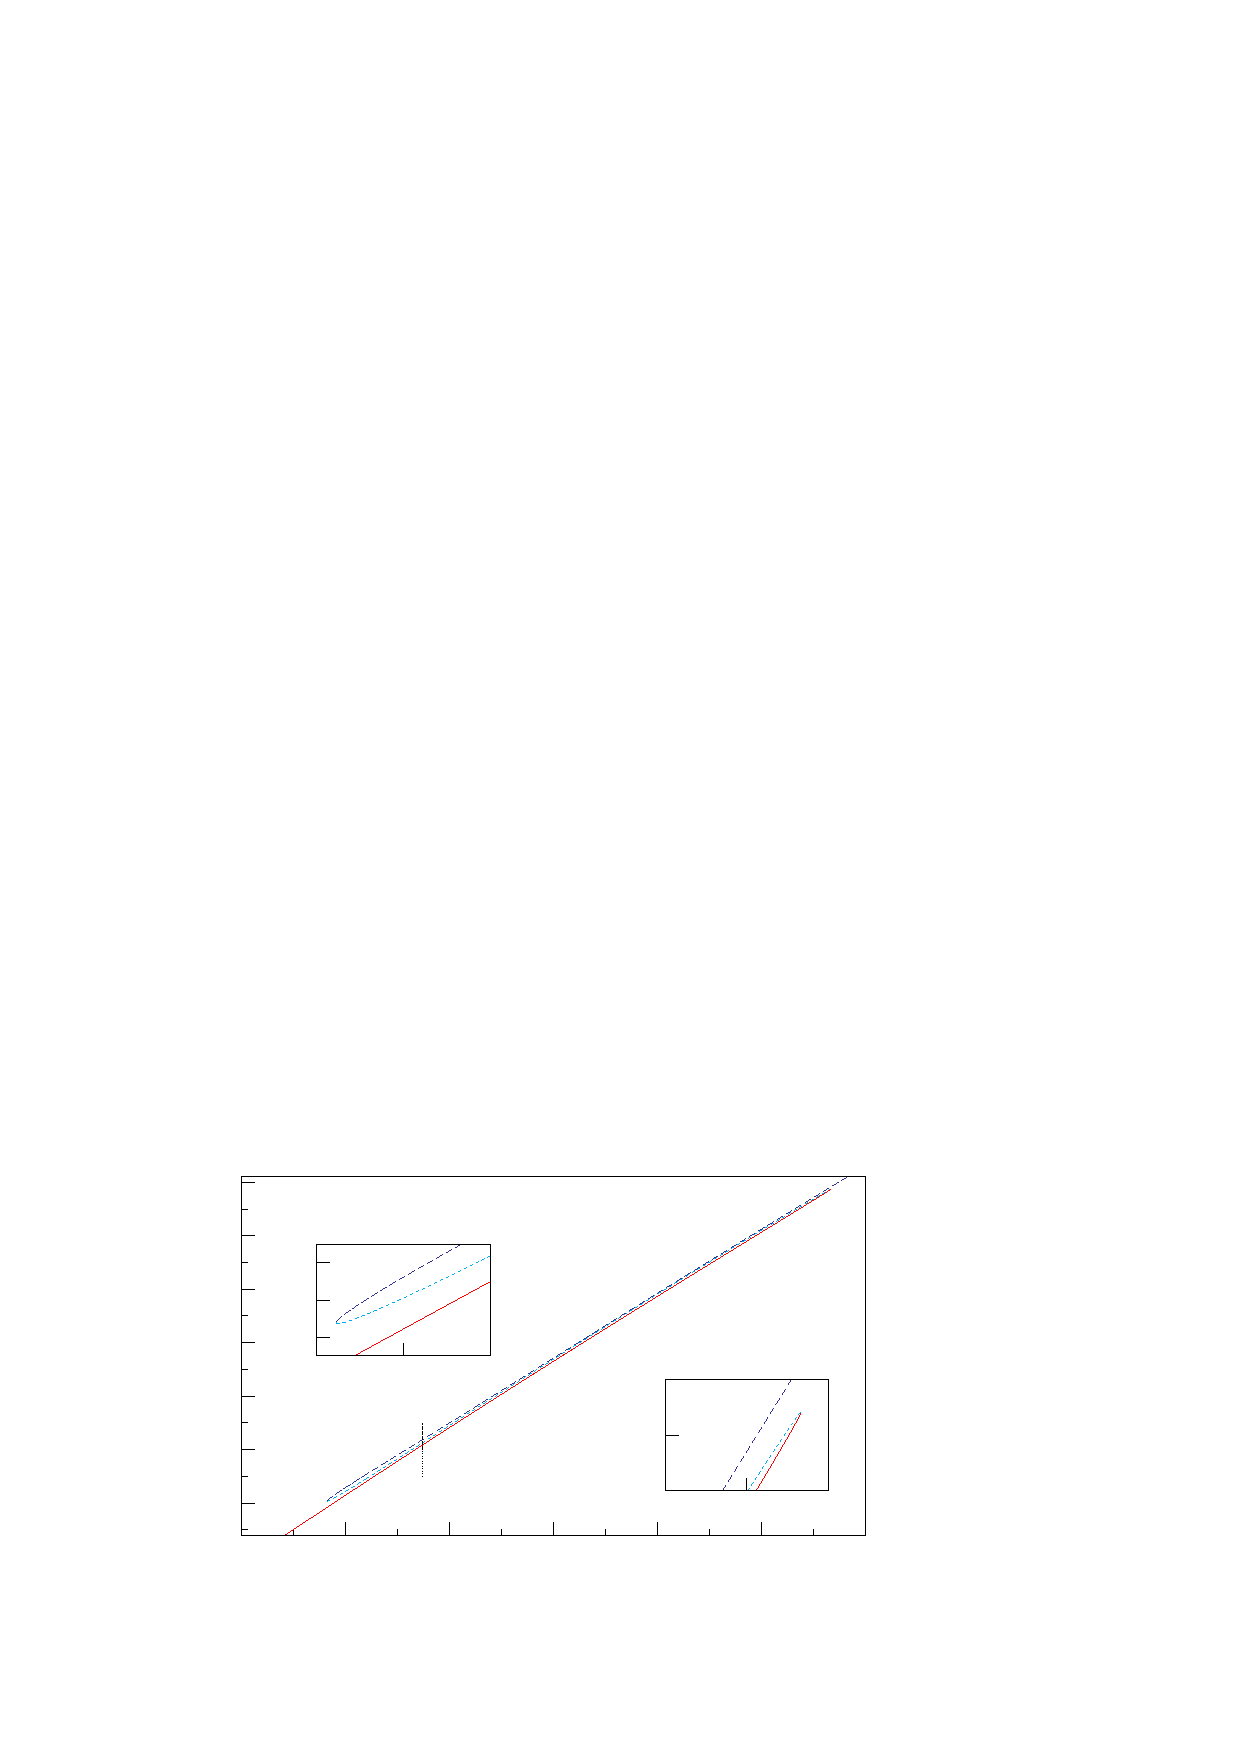
\includegraphics{Images/epslatex/lp_branches}%
\end{picture}%
\begingroup
\setlength{\unitlength}{0.0200bp}%
\begin{picture}(18000,10800)(0,0)%
\put(1925,2420){\makebox(0,0)[r]{\strut{} 23}}%
\put(1925,3704){\makebox(0,0)[r]{\strut{} 24}}%
\put(1925,4987){\makebox(0,0)[r]{\strut{} 25}}%
\put(1925,6271){\makebox(0,0)[r]{\strut{} 26}}%
\put(1925,7554){\makebox(0,0)[r]{\strut{} 27}}%
\put(1925,8838){\makebox(0,0)[r]{\strut{} 28}}%
\put(1925,10122){\makebox(0,0)[r]{\strut{} 29}}%
\put(2200,1100){\makebox(0,0){\strut{} 1.75}}%
\put(4696,1100){\makebox(0,0){\strut{} 1.8}}%
\put(7192,1100){\makebox(0,0){\strut{} 1.85}}%
\put(9688,1100){\makebox(0,0){\strut{} 1.9}}%
\put(12183,1100){\makebox(0,0){\strut{} 1.95}}%
\put(14679,1100){\makebox(0,0){\strut{} 2}}%
\put(17175,1100){\makebox(0,0){\strut{} 2.05}}%
\put(550,5950){\rotatebox{90}{\makebox(0,0){\strut{}$\mathcal{\tilde{D}}$}}}%
\put(9687,275){\makebox(0,0){\strut{}$m$}}%
\put(3725,8185){\makebox(0,0)[r]{\strut{} 23.2}}%
\put(3725,7295){\makebox(0,0)[r]{\strut{} 23.1}}%
\put(3725,6405){\makebox(0,0)[r]{\strut{} 23}}%
\put(8175,5410){\makebox(0,0){\strut{} 1.8}}%
\put(6087,5410){\makebox(0,0){\strut{} 1.795}}%
\put(4000,5410){\makebox(0,0){\strut{} 1.79}}%
\put(12100,5390){\makebox(0,0)[r]{\strut{} 28.9}}%
\put(12100,4055){\makebox(0,0)[r]{\strut{} 28.85}}%
\put(12100,2720){\makebox(0,0)[r]{\strut{} 28.8}}%
\put(16275,2170){\makebox(0,0){\strut{} 2.035}}%
\put(14325,2170){\makebox(0,0){\strut{} 2.03}}%
\put(12375,2170){\makebox(0,0){\strut{} 2.025}}%
\end{picture}%
\endgroup
\endinput

\end{center}
\caption[Branches of bimodals]{\baselineskip=1.0\normalbaselineskip%
Three connected bimodal branches $b_{1}$ (dark blue), $b_{2}$ (light blue) and $b_{3}$ (red) at $\lambda=0.20$ with $\nu={1}\slash{3}$ and $\epsilon=0.1$. From continuation in $m$ the branches $b_{1}$ and $b_{2}$ coalesce at $m=1.791139$, while the $b_{2}$ and $b_{3}$ curves coalesce at $m=2.033325$. The dashed line marks the point at which $b_{2}$ switches from connecting $b_{2}$ and $b_{3}$.}
\label{fig:lp_branches}
\end{figure}
% 
\par % Specifics of one branch
The figure~\ref{fig:lp_branches} shows the continuation of a solution at $m=1.81$, $\lambda=0.20$ in $m$. There are three branches, labelled $b_{1}$, $b_{2}$ and $b_{3}$ connected by two limit points at $lp_{1}=\left(0.2,1.791139\right)$ and $lp_{1}=\left(0.2,2.033325\right)$.  Branch $b_{1}$ can be continued further with $m$ increasing and branch $b_{3}$ be continued in $m$ decreasing. However it is the behaviour of the middle branch $b_{2}$ which is of interest as it connects both branches. 
%
\par
In the neighbourhood of the limit point $lp_{1}$ continuation in $\lambda$ from branch $b_{1}$ reaches a limit point and then heads back on to branch $b_{2}$. Figure~\ref{fig:shell} illustrates the phenomena described: continuation in $\lambda$ (purple) for a range of values of $m$ shows the connection between branches $b_{1}$ (in dark blue) and $b_{2}$ (in light blue). Similarly in the neighbourhood of $lp_{2}$ so the two branches $b_{2}$ and $b_{3}$ (in red) are connected when continuation is performed in $\lambda$. 
%
\begin{figure}[h!tbp]
\begin{center}
%GNUPLOT: LaTeX picture with Postscript
\begin{picture}(0,0)%
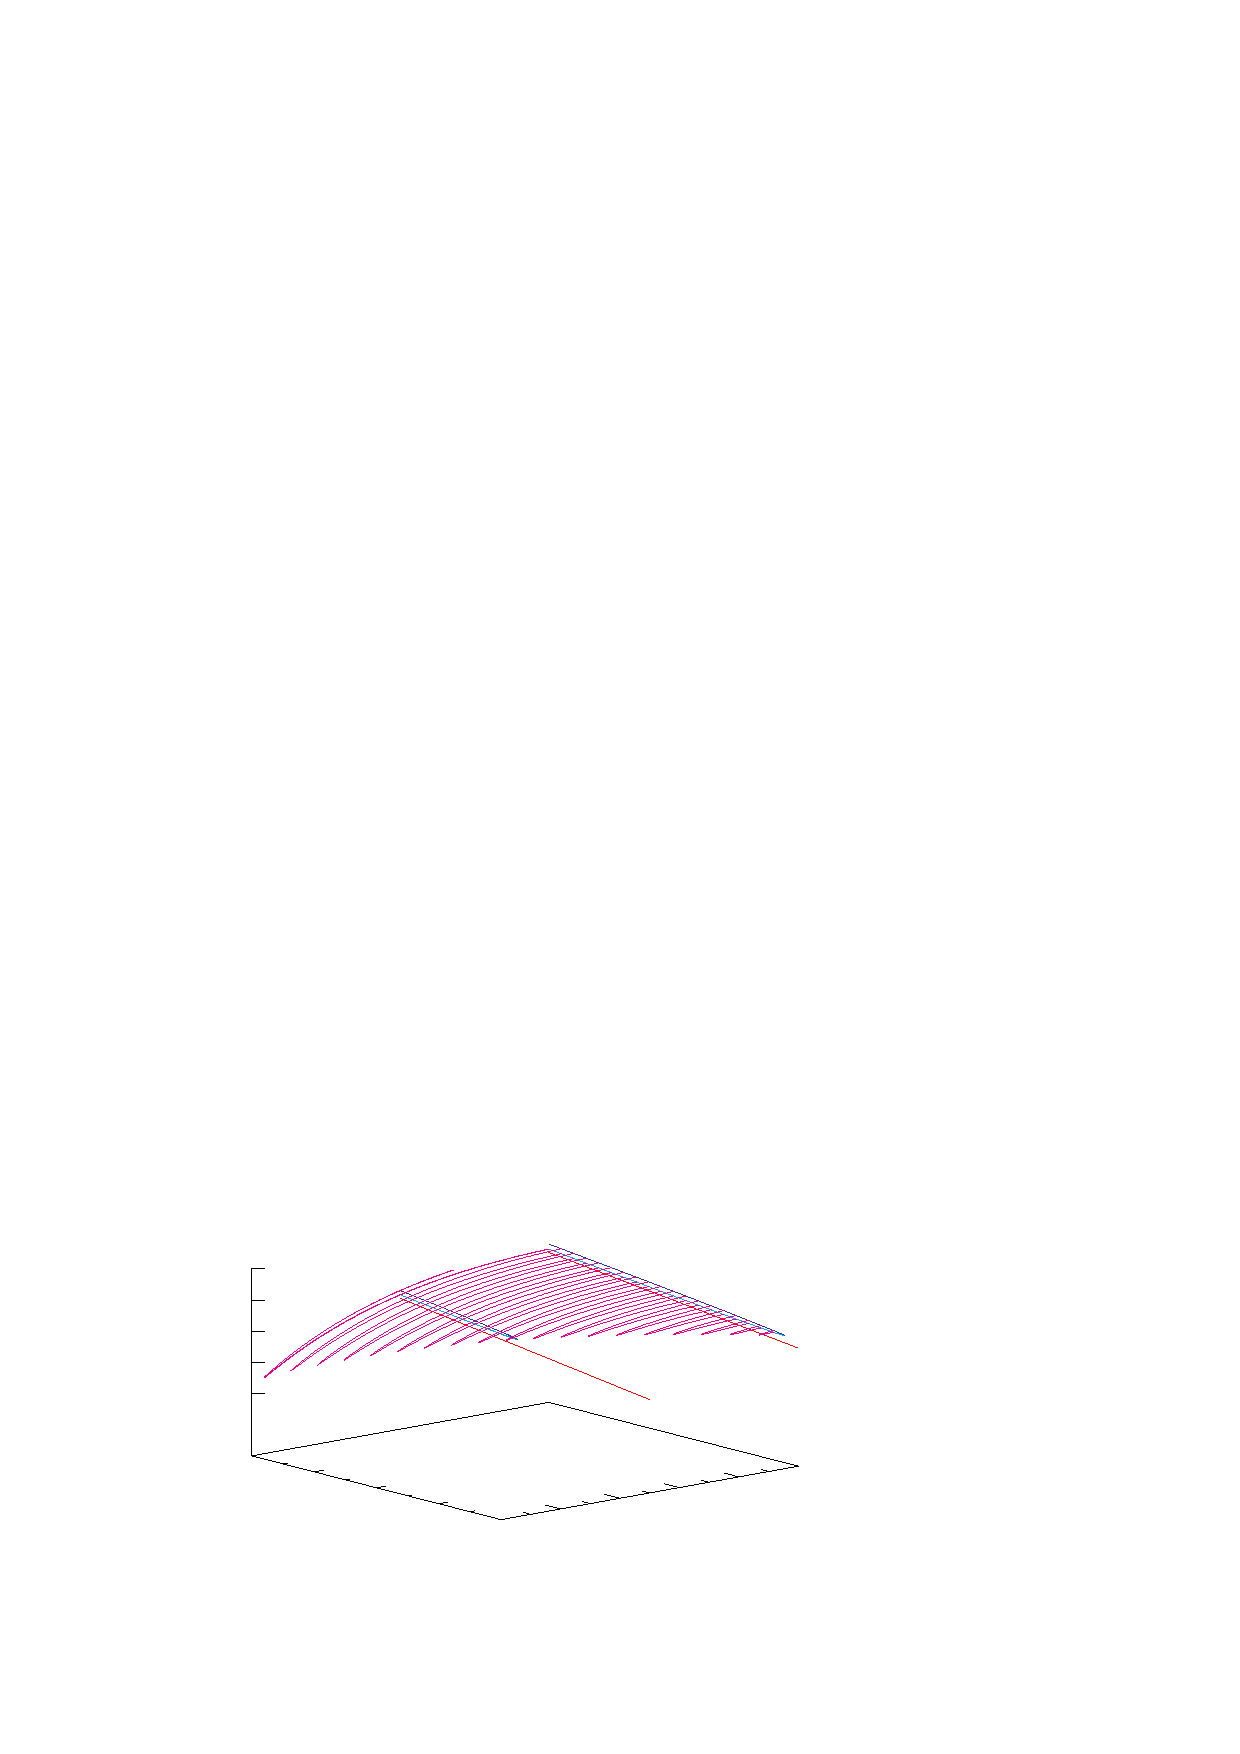
\includegraphics{Images/epslatex/shell}%
\end{picture}%
\begingroup
\setlength{\unitlength}{0.0200bp}%
\begin{picture}(18000,10800)(0,0)%
\put(8762,1852){\makebox(0,0)[l]{\strut{} 0.15}}%
\put(10188,2109){\makebox(0,0)[l]{\strut{} 0.16}}%
\put(11615,2366){\makebox(0,0)[l]{\strut{} 0.17}}%
\put(13042,2623){\makebox(0,0)[l]{\strut{} 0.18}}%
\put(14469,2880){\makebox(0,0)[l]{\strut{} 0.19}}%
\put(15896,3137){\makebox(0,0)[l]{\strut{} 0.2}}%
\put(8216,1948){\makebox(0,0){\strut{} 1.79}}%
\put(6719,2331){\makebox(0,0){\strut{} 1.795}}%
\put(5222,2713){\makebox(0,0){\strut{} 1.8}}%
\put(3726,3096){\makebox(0,0){\strut{} 1.805}}%
\put(2229,3479){\makebox(0,0){\strut{} 1.81}}%
\put(1840,8042){\makebox(0,0)[r]{\strut{} 24}}%
\put(1840,7294){\makebox(0,0)[r]{\strut{} 23.5}}%
\put(1840,6546){\makebox(0,0)[r]{\strut{} 23}}%
\put(1840,5798){\makebox(0,0)[r]{\strut{} 22.5}}%
\put(1840,5051){\makebox(0,0)[r]{\strut{} 22}}%
\put(2439,9164){\makebox(0,0){\strut{}$\tilde{\mathcal{D}}$}}%
\put(13215,1733){\makebox(0,0){\strut{}$\lambda$}}%
\put(3649,2468){\makebox(0,0){\strut{}$m$}}%
\put(2439,9164){\makebox(0,0){\strut{}$\tilde{\mathcal{D}}$}}%
\end{picture}%
\endgroup
\endinput

\end{center}
\caption[Connected branches of bimodals]{\baselineskip=1.0\normalbaselineskip%
Continuation in $m$ and $\lambda$ showing a succession of coalescence curves (purple) connecting the branches $b_{1}$ (dark blue) and $b_{2}$ (light blue) when $\epsilon=0.1$ and $\nu=1\slash{3}$.}
\label{fig:shell}
\end{figure}
%
\par % Limit point switching
Numerical investigation presented in figure~\ref{fig:lambda_many} reveals that when continuation is performed with $\lambda$ decreasing from $\lambda=0.20$, that for $lp_{1}<m<1.837$ the branch $b_{2}$ connects $b_{1}$ (in dark blue) but for $1.837<m<lp_{2}$ the branch $b_{2}$ now connects $b_{3}$ (in red).  The branch $b_{2}$ switches from connecting $b_{1}$ to connecting $b_{3}$. At $m=1.837$ the load-deflection diagrams are minimal, as illustrated by subfigure~\ref{fig:lambda_many_D}.  As shown in subfigure~\ref{fig:lambda_many_T} the truncated arclength is greatest at this point. 
%
\begin{figure}[h!tbp]
\begin{center}
\subfigure[][]{ %GNUPLOT: LaTeX picture with Postscript
\begin{picture}(0,0)%
\includegraphics{Images/epslatex/lambda_many_D}%
\end{picture}%
\begingroup
\setlength{\unitlength}{0.0200bp}%
\begin{picture}(9900,6480)(0,0)%
\put(1925,1650){\makebox(0,0)[r]{\strut{} 12}}%
\put(1925,2126){\makebox(0,0)[r]{\strut{} 14}}%
\put(1925,2601){\makebox(0,0)[r]{\strut{} 16}}%
\put(1925,3077){\makebox(0,0)[r]{\strut{} 18}}%
\put(1925,3552){\makebox(0,0)[r]{\strut{} 20}}%
\put(1925,4028){\makebox(0,0)[r]{\strut{} 22}}%
\put(1925,4503){\makebox(0,0)[r]{\strut{} 24}}%
\put(1925,4979){\makebox(0,0)[r]{\strut{} 26}}%
\put(1925,5454){\makebox(0,0)[r]{\strut{} 28}}%
\put(1925,5930){\makebox(0,0)[r]{\strut{} 30}}%
\put(2200,1100){\makebox(0,0){\strut{} 0.1}}%
\put(3575,1100){\makebox(0,0){\strut{} 0.12}}%
\put(4950,1100){\makebox(0,0){\strut{} 0.14}}%
\put(6325,1100){\makebox(0,0){\strut{} 0.16}}%
\put(7700,1100){\makebox(0,0){\strut{} 0.18}}%
\put(9075,1100){\makebox(0,0){\strut{} 0.2}}%
\put(550,3790){\rotatebox{90}{\makebox(0,0){\strut{}$\tilde{\mathcal{D}}$}}}%
\put(5637,275){\makebox(0,0){\strut{}$\lambda$}}%
\end{picture}%
\endgroup
\endinput
 \label{fig:lambda_many_D} }
\subfigure[][]{ %GNUPLOT: LaTeX picture with Postscript
\begin{picture}(0,0)%
\includegraphics{Images/epslatex/lambda_many_T}%
\end{picture}%
\begingroup
\setlength{\unitlength}{0.0200bp}%
\begin{picture}(9900,6480)(0,0)%
\put(2475,1650){\makebox(0,0)[r]{\strut{} 57}}%
\put(2475,2261){\makebox(0,0)[r]{\strut{} 57.5}}%
\put(2475,2873){\makebox(0,0)[r]{\strut{} 58}}%
\put(2475,3484){\makebox(0,0)[r]{\strut{} 58.5}}%
\put(2475,4096){\makebox(0,0)[r]{\strut{} 59}}%
\put(2475,4707){\makebox(0,0)[r]{\strut{} 59.5}}%
\put(2475,5319){\makebox(0,0)[r]{\strut{} 60}}%
\put(2475,5930){\makebox(0,0)[r]{\strut{} 60.5}}%
\put(2750,1100){\makebox(0,0){\strut{} 0.1}}%
\put(4015,1100){\makebox(0,0){\strut{} 0.12}}%
\put(5280,1100){\makebox(0,0){\strut{} 0.14}}%
\put(6545,1100){\makebox(0,0){\strut{} 0.16}}%
\put(7810,1100){\makebox(0,0){\strut{} 0.18}}%
\put(9075,1100){\makebox(0,0){\strut{} 0.2}}%
\put(550,3790){\rotatebox{90}{\makebox(0,0){\strut{}$\mathcal{T}$}}}%
\put(5912,275){\makebox(0,0){\strut{}$\lambda$}}%
\end{picture}%
\endgroup
\endinput
 \label{fig:lambda_many_T} }
\end{center}
\caption[End shortening and truncation length for bimodals]{\baselineskip=1.0\normalbaselineskip%
Subfigure~\ref{fig:lambda_many_D} shows load deflection diagrams for bimodal configurations for a range of $m$ when continued under $\lambda$. The red curves are those with $m~\ge~1.837$ and thus connect $b_{2}$ to $b_{3}$ whereas the dark blue curves connect $b_{1}$ and $b_{2}$ as $m~\le~1.837$. Subfigure~\ref{fig:lambda_many_T} shows how the truncated arclength increases as the delocalisation increases as $m$ approaches $1.837$ from the left and the right.}  
\label{fig:lambda_many}
\end{figure}
% 
\par % Differing configurations
By the previous coalescence rules, as $b_{1}$ in connected to $b_{2}$ which in turn then connects $b_{3}$, so the two branches $b_{1}$ and $b_{3}$ should be the same. Figure~\ref{fig:xfort} shows the configurations, using the same colour scheme, on the three branches at fixed values of $m$. A number of observations can be made, firstly note that the configurations displayed in subfigures~\ref{fig:xfort.22} and~\ref{fig:xfort.21} and those in subfigures~\ref{fig:xfort.23} and~\ref{fig:xfort.24} are qualitatively similar as the values of $m$ are near the limit points at which they coalesce. Also, it is evident that configurations on branch $b_{1}$ have more quarter turns those on $b_{3}$. It is also clear that on branch $b_{2}$ subfigure~\ref{fig:xfort.21} has the same number of turns as subfigures~\ref{fig:xfort.22} and~\ref{fig:xfort.25} on branch $b_{1}$. Similarly, subfigure~\ref{fig:xfort.23} on branch $b_{2}$ has the same number of turns as subfigures~\ref{fig:xfort.26} and~\ref{fig:xfort.24} on branch $b_{1}$. Thus, the discontinuity the truncation length of the configurations along branch $b_{2}$, as illustrated in subfigure~\ref{fig:lambda_many_T}, is due to an increase the number of quarter turns on the branch of bimodals.
%
\begin{figure}[h!tbp]
\begin{center}
\subfigure[][$b_{1}$, $m=1.80$]{ \input{Images/epslatex/xfort.22.tex} \label{fig:xfort.22} }
\subfigure[][$b_{1}$, $m=2.00$]{ \input{Images/epslatex/xfort.25.tex} \label{fig:xfort.25} }
\subfigure[][$b_{2}$, $m=1.80$]{ \input{Images/epslatex/xfort.21.tex} \label{fig:xfort.21} }
\subfigure[][$b_{2}$, $m=2.00$]{ \input{Images/epslatex/xfort.23.tex} \label{fig:xfort.23} }
\subfigure[][$b_{3}$, $m=1.80$]{ \input{Images/epslatex/xfort.26.tex} \label{fig:xfort.26} }
\subfigure[][$b_{3}$, $m=2.00$]{ \input{Images/epslatex/xfort.24.tex} \label{fig:xfort.24} }
\end{center}
\caption[Bimodal configurations on connected branches]{\baselineskip=1.0\normalbaselineskip%
Bimodal configurations on the connected branches in figure~\ref{fig:lp_branches}.}  
\label{fig:xfort}
\end{figure}
% 
\par % Other branches
Branch $b_{3}$ then approaches $\lambda_{c}^{\left(2\right)}$ and passes beyond it merging with other isolae. The branches $b_{2}$ and $b_{1}$ cannot pass through the codimension-two point  and instead reach limit points.  In order to merge with other branches branches $b_{1}$ and $b_{2}$ must be continued in $m$ onto branch $b_{3}$, as in figure~\ref{fig:lp}. As has been observed, the branch $b_{3}$ appears to have a fewer number quarter turns than branches $b_{2}$ and $b_{1}$ and, as was seen in figure~\ref{fig:bi_lp} in the anisotropic Kirchhoff rod, bimodals with smaller gaps between localisations can be continued further towards the codimension-two point.
%
\par 
While the results presented here hold for other bimodals, without analytical results the numerical evidence provides an insight into one branch in a multiplicity of homoclinic solutions.  A rich bifurcation structure clearly exists, for example, just beyond $lp_{2}$ the branch $b_{1}$ connects, through continuation in $\lambda$, with another distinct branch at $\left(0.2,1.975411\right)$. This new branch possesses limit points both forward and backward in $m$ and its load-deflection diagrams do not resemble figure~\ref{fig:lp_branches}.
%
\par % Spectrum of limit points
The $\left(\lambda,m\right)$ parameter space was explored and collection of limit points discovered. The results are presented in figure~\ref{fig:spectrum}. Again, note the figure may not give an global picture of the bifurcation structure of the bimodals as continuation was performed manually from a single solution. It should be noted that in this figure the only limit points which are expected (from linear analysis) are those which approach the buckling line such as $lp_{1}$ rather than those which are away from the buckling line such as $lp_{2}$. A similar set of results should be expected for solutions with small $\lambda$ to the left of the elliptic region, but pairs of limit points should be expected one approaching the buckling line another in the anti-integrable limit.
% 
\begin{figure}[h!tbp]
\begin{center}
\subfigure[][$m=1.81$]{
%GNUPLOT: LaTeX picture with Postscript
\begin{picture}(0,0)%
\includegraphics{Images/epslatex/R_cusp}%
\end{picture}%
\begingroup
\setlength{\unitlength}{0.0200bp}%
\begin{picture}(9900,6480)(0,0)%
\put(2200,1650){\makebox(0,0)[r]{\strut{} 1}}%
\put(2200,2261){\makebox(0,0)[r]{\strut{} 1.1}}%
\put(2200,2873){\makebox(0,0)[r]{\strut{} 1.2}}%
\put(2200,3484){\makebox(0,0)[r]{\strut{} 1.3}}%
\put(2200,4096){\makebox(0,0)[r]{\strut{} 1.4}}%
\put(2200,4707){\makebox(0,0)[r]{\strut{} 1.5}}%
\put(2200,5319){\makebox(0,0)[r]{\strut{} 1.6}}%
\put(2200,5930){\makebox(0,0)[r]{\strut{} 1.7}}%
\put(3192,1100){\makebox(0,0){\strut{} 0.15}}%
\put(4627,1100){\makebox(0,0){\strut{} 0.2}}%
\put(6062,1100){\makebox(0,0){\strut{} 0.25}}%
\put(7497,1100){\makebox(0,0){\strut{} 0.3}}%
\put(8932,1100){\makebox(0,0){\strut{} 0.35}}%
\put(550,3790){\rotatebox{90}{\makebox(0,0){\strut{}$\tilde{\mathcal{R}}$}}}%
\put(5775,275){\makebox(0,0){\strut{}$\lambda$}}%
\end{picture}%
\endgroup
\endinput

%GNUPLOT: LaTeX picture with Postscript
\begin{picture}(0,0)%
\includegraphics{Images/epslatex/D_cusp}%
\end{picture}%
\begingroup
\setlength{\unitlength}{0.0200bp}%
\begin{picture}(9900,6480)(0,0)%
\put(2475,1650){\makebox(0,0)[r]{\strut{} 21.6}}%
\put(2475,2078){\makebox(0,0)[r]{\strut{} 21.8}}%
\put(2475,2506){\makebox(0,0)[r]{\strut{} 22}}%
\put(2475,2934){\makebox(0,0)[r]{\strut{} 22.2}}%
\put(2475,3362){\makebox(0,0)[r]{\strut{} 22.4}}%
\put(2475,3790){\makebox(0,0)[r]{\strut{} 22.6}}%
\put(2475,4218){\makebox(0,0)[r]{\strut{} 22.8}}%
\put(2475,4646){\makebox(0,0)[r]{\strut{} 23}}%
\put(2475,5074){\makebox(0,0)[r]{\strut{} 23.2}}%
\put(2475,5502){\makebox(0,0)[r]{\strut{} 23.4}}%
\put(2475,5930){\makebox(0,0)[r]{\strut{} 23.6}}%
\put(3438,1100){\makebox(0,0){\strut{} 0.15}}%
\put(4813,1100){\makebox(0,0){\strut{} 0.2}}%
\put(6188,1100){\makebox(0,0){\strut{} 0.25}}%
\put(7563,1100){\makebox(0,0){\strut{} 0.3}}%
\put(8938,1100){\makebox(0,0){\strut{} 0.35}}%
\put(550,3790){\rotatebox{90}{\makebox(0,0){\strut{}$\tilde{\mathcal{D}}$}}}%
\put(5912,275){\makebox(0,0){\strut{}$\lambda$}}%
\end{picture}%
\endgroup
\endinput
 \label{fig:cusp} }
\subfigure[][$m=1.91$]{
%GNUPLOT: LaTeX picture with Postscript
\begin{picture}(0,0)%
\includegraphics{Images/epslatex/R_coalescence}%
\end{picture}%
\begingroup
\setlength{\unitlength}{0.0200bp}%
\begin{picture}(9900,6480)(0,0)%
\put(2475,1650){\makebox(0,0)[r]{\strut{} 0.55}}%
\put(2475,2185){\makebox(0,0)[r]{\strut{} 0.6}}%
\put(2475,2720){\makebox(0,0)[r]{\strut{} 0.65}}%
\put(2475,3255){\makebox(0,0)[r]{\strut{} 0.7}}%
\put(2475,3790){\makebox(0,0)[r]{\strut{} 0.75}}%
\put(2475,4325){\makebox(0,0)[r]{\strut{} 0.8}}%
\put(2475,4860){\makebox(0,0)[r]{\strut{} 0.85}}%
\put(2475,5395){\makebox(0,0)[r]{\strut{} 0.9}}%
\put(2475,5930){\makebox(0,0)[r]{\strut{} 0.95}}%
\put(2750,1100){\makebox(0,0){\strut{} 0.095}}%
\put(3804,1100){\makebox(0,0){\strut{} 0.1}}%
\put(4858,1100){\makebox(0,0){\strut{} 0.105}}%
\put(5913,1100){\makebox(0,0){\strut{} 0.11}}%
\put(6967,1100){\makebox(0,0){\strut{} 0.115}}%
\put(8021,1100){\makebox(0,0){\strut{} 0.12}}%
\put(9075,1100){\makebox(0,0){\strut{} 0.125}}%
\put(550,3790){\rotatebox{90}{\makebox(0,0){\strut{}$\tilde{\mathcal{R}}$}}}%
\put(5912,275){\makebox(0,0){\strut{}$\lambda$}}%
\end{picture}%
\endgroup
\endinput
 
%GNUPLOT: LaTeX picture with Postscript
\begin{picture}(0,0)%
\includegraphics{Images/epslatex/D_coalescence}%
\end{picture}%
\begingroup
\setlength{\unitlength}{0.0200bp}%
\begin{picture}(9900,6480)(0,0)%
\put(1925,1650){\makebox(0,0)[r]{\strut{} 15}}%
\put(1925,2126){\makebox(0,0)[r]{\strut{} 16}}%
\put(1925,2601){\makebox(0,0)[r]{\strut{} 17}}%
\put(1925,3077){\makebox(0,0)[r]{\strut{} 18}}%
\put(1925,3552){\makebox(0,0)[r]{\strut{} 19}}%
\put(1925,4028){\makebox(0,0)[r]{\strut{} 20}}%
\put(1925,4503){\makebox(0,0)[r]{\strut{} 21}}%
\put(1925,4979){\makebox(0,0)[r]{\strut{} 22}}%
\put(1925,5454){\makebox(0,0)[r]{\strut{} 23}}%
\put(1925,5930){\makebox(0,0)[r]{\strut{} 24}}%
\put(2200,1100){\makebox(0,0){\strut{} 0.095}}%
\put(3346,1100){\makebox(0,0){\strut{} 0.1}}%
\put(4492,1100){\makebox(0,0){\strut{} 0.105}}%
\put(5638,1100){\makebox(0,0){\strut{} 0.11}}%
\put(6783,1100){\makebox(0,0){\strut{} 0.115}}%
\put(7929,1100){\makebox(0,0){\strut{} 0.12}}%
\put(9075,1100){\makebox(0,0){\strut{} 0.125}}%
\put(550,3790){\rotatebox{90}{\makebox(0,0){\strut{}$\tilde{\mathcal{D}}$}}}%
\put(5637,275){\makebox(0,0){\strut{}$\lambda$}}%
\end{picture}%
\endgroup
\endinput
 \label{fig:coalescence} }
\subfigure[][$m=2.00$]{
%GNUPLOT: LaTeX picture with Postscript
\begin{picture}(0,0)%
\includegraphics{Images/epslatex/R_dovetail}%
\end{picture}%
\begingroup
\setlength{\unitlength}{0.0200bp}%
\begin{picture}(9900,6480)(0,0)%
\put(2200,1650){\makebox(0,0)[r]{\strut{} 0.8}}%
\put(2200,2126){\makebox(0,0)[r]{\strut{} 0.9}}%
\put(2200,2601){\makebox(0,0)[r]{\strut{} 1}}%
\put(2200,3077){\makebox(0,0)[r]{\strut{} 1.1}}%
\put(2200,3552){\makebox(0,0)[r]{\strut{} 1.2}}%
\put(2200,4028){\makebox(0,0)[r]{\strut{} 1.3}}%
\put(2200,4503){\makebox(0,0)[r]{\strut{} 1.4}}%
\put(2200,4979){\makebox(0,0)[r]{\strut{} 1.5}}%
\put(2200,5454){\makebox(0,0)[r]{\strut{} 1.6}}%
\put(2200,5930){\makebox(0,0)[r]{\strut{} 1.7}}%
\put(2475,1100){\makebox(0,0){\strut{} 0.1}}%
\put(3795,1100){\makebox(0,0){\strut{} 0.15}}%
\put(5115,1100){\makebox(0,0){\strut{} 0.2}}%
\put(6435,1100){\makebox(0,0){\strut{} 0.25}}%
\put(7755,1100){\makebox(0,0){\strut{} 0.3}}%
\put(9075,1100){\makebox(0,0){\strut{} 0.35}}%
\put(550,3790){\rotatebox{90}{\makebox(0,0){\strut{}$\tilde{\mathcal{R}}$}}}%
\put(5775,275){\makebox(0,0){\strut{}$\lambda$}}%
\end{picture}%
\endgroup
\endinput

%GNUPLOT: LaTeX picture with Postscript
\begin{picture}(0,0)%
\includegraphics{Images/epslatex/D_dovetail}%
\end{picture}%
\begingroup
\setlength{\unitlength}{0.0200bp}%
\begin{picture}(9900,6480)(0,0)%
\put(2475,1650){\makebox(0,0)[r]{\strut{} 24.5}}%
\put(2475,2126){\makebox(0,0)[r]{\strut{} 25}}%
\put(2475,2601){\makebox(0,0)[r]{\strut{} 25.5}}%
\put(2475,3077){\makebox(0,0)[r]{\strut{} 26}}%
\put(2475,3552){\makebox(0,0)[r]{\strut{} 26.5}}%
\put(2475,4028){\makebox(0,0)[r]{\strut{} 27}}%
\put(2475,4503){\makebox(0,0)[r]{\strut{} 27.5}}%
\put(2475,4979){\makebox(0,0)[r]{\strut{} 28}}%
\put(2475,5454){\makebox(0,0)[r]{\strut{} 28.5}}%
\put(2475,5930){\makebox(0,0)[r]{\strut{} 29}}%
\put(2750,1100){\makebox(0,0){\strut{} 0.1}}%
\put(4015,1100){\makebox(0,0){\strut{} 0.15}}%
\put(5280,1100){\makebox(0,0){\strut{} 0.2}}%
\put(6545,1100){\makebox(0,0){\strut{} 0.25}}%
\put(7810,1100){\makebox(0,0){\strut{} 0.3}}%
\put(9075,1100){\makebox(0,0){\strut{} 0.35}}%
\put(550,3790){\rotatebox{90}{\makebox(0,0){\strut{}$\tilde{\mathcal{D}}$}}}%
\put(5912,275){\makebox(0,0){\strut{}$\lambda$}}%
\end{picture}%
\endgroup
\endinput
 \label{fig:dovetail} }
\caption[Load-deflections]{\baselineskip=1.0\normalbaselineskip%
A variety of load-deflection diagrams for $\lambda$ showing different classes of bifurcation diagram.}
\label{fig:load_deflections}
\end{center}
\end{figure}
% 
\begin{figure}[h!tbp]
\begin{center}
%GNUPLOT: LaTeX picture with Postscript
\begin{picture}(0,0)%
\includegraphics{Images/epslatex/spectrum}%
\end{picture}%
\begingroup
\setlength{\unitlength}{0.0200bp}%
\begin{picture}(18000,10800)(0,0)%
\put(2475,1650){\makebox(0,0)[r]{\strut{} 1.75}}%
\put(2475,2879){\makebox(0,0)[r]{\strut{} 1.8}}%
\put(2475,4107){\makebox(0,0)[r]{\strut{} 1.85}}%
\put(2475,5336){\makebox(0,0)[r]{\strut{} 1.9}}%
\put(2475,6564){\makebox(0,0)[r]{\strut{} 1.95}}%
\put(2475,7793){\makebox(0,0)[r]{\strut{} 2}}%
\put(2475,9021){\makebox(0,0)[r]{\strut{} 2.05}}%
\put(2475,10250){\makebox(0,0)[r]{\strut{} 2.1}}%
\put(2750,1100){\makebox(0,0){\strut{} 0}}%
\put(5154,1100){\makebox(0,0){\strut{} 0.05}}%
\put(7558,1100){\makebox(0,0){\strut{} 0.1}}%
\put(9963,1100){\makebox(0,0){\strut{} 0.15}}%
\put(12367,1100){\makebox(0,0){\strut{} 0.2}}%
\put(14771,1100){\makebox(0,0){\strut{} 0.25}}%
\put(17175,1100){\makebox(0,0){\strut{} 0.3}}%
\put(550,5950){\rotatebox{90}{\makebox(0,0){\strut{}$m$}}}%
\put(9962,275){\makebox(0,0){\strut{}$\lambda$}}%
\end{picture}%
\endgroup
\endinput
 % ...auto/Magnetic/LP/Data
\end{center}
\caption[Limit points of a bimodal]{\baselineskip=1.0\normalbaselineskip%
A succession of limit points for a set of bimodals against the spectrum of Floquet multipliers when $\epsilon=0.1$ and $\nu=1\slash{3}$. As in figure~\ref{fig:lambda_spectrum} the shaded area is the elliptic regime and the dotted line the codimension-one curve~\eqref{eq:codim_one_curve}.}
\label{fig:spectrum}
\end{figure}
%
%---------------------------------------------
%
% The Rule of three: this is the last part.
%
%---------------------------------------------
%
\chapter{Conclusion} \label{chap:conc}
%
\par % Description of this chapter
The objective of this thesis was to investigate the behaviour of a conducting elastic rod in a magnetic field and a number of original contributions have been made. Firstly, the identification of the static equilibrium equations as a noncanonical Hamiltonian system which for a class of constitutive relations is completely integrable. Secondly, through detailed perturbation analysis it is shown that it is the direct coupling of the magnetic effects and extensibility leads to spatial chaos. Thirdly, the existence of a codimension-two Hamiltonian Hopf-Hopf bifurcation and its role as an organising centre for the nearby dynamics.  %  
%
\par % Discussion - Hamiltonian formulation
Perhaps the most important step in the analysis was recognising that the static equilibrium equations were a noncanonical system as the Hamiltonian structure is emphasised and exploited throughout this thesis. For example, the Hamiltonian structure is necessary in order to prove complete integrability in the unperturbed system, in the reduction to a canonical system, in the Mel'nikov analysis and, by exploiting the codimension of homoclinic solutions in Hamiltonian systems, to produce load-deflection diagrams.
%
\par % Summary - integrability
The equilibrium equations are, like the Kirchhoff equations, Lie-Poisson equations. It is shown that the new Lie-Poisson bracket is produced via Liebniz and semidirect extensions to the Kirchhoff bracket. The bracket extensions are generalised and the equilibrium equations found to sit, as the third member, in a family of rod equations in generalised magnetic fields. Thus, the rod in a uniform magnetic field gives a physical realisation to the abstract `Twisted top'~\cite{Thiffeault01}. Interestingly, the Hamiltonian remains unchanged and effect of the magnetic field is contained within the structure matrix. A new and rather pleasing observation is that the contributions of each generalised force on the rod is a provided by a nontrivial bracket extension. %
% 
\par % Summary - bracket
However, it is the form of the Poisson bracket which presents a major obstacle in the analysis. A complete interpretation of all of the symmetry laws which determine the integrals would allow, through a suitable parameterisation, a reduction to a single degree of freedom system. Such a reduction would then allow the homoclinic orbits to be expressed in closed form, the application of Mel'nikov analysis when extensibility is the perturbation parameter, action-angle variables to be constructed and closed form expressions for the buckling loads. % For Lie-Poisson equations with a symmetry law, using infinitesimal generators on a suitable inner product, conserved quantities can be found~\cite{Simo90}. However, there is no algorithmic procedure which from a conserved quantity associates a symmetry. %
% 
\par % Discussion - structure of the force
The equilibrium equations are shown to be integrable for a class of constitutive relations. Thus, when a rod is ordinarily straight, linearly elastic, isotropic, inextensible and unshearable and a generalised force of the form $\boldsymbol{F}\times\boldsymbol{d}_{3}$, i.e., some field $\boldsymbol{F}$ acts normal to the rod, then the resulting system is integrable. The integrable subfamily of equations is then parameterised by a Lax pair. 
%
\par % Discussion - Hidden conditions of the Lax pair
The Lax pair formulation reveals hidden conditions on the constitutive relations in order for all the members of the family of rod equations to be integrable. For example, the force-free is (super)integrable regardless of isotropy or nonlinear constitutive relations, in contrast to the Kirchhoff rod which requires isotropy in order to be integrable. The rod in a magnetic field now requires the addition conditions of inextensibility, unshearability and linear elasticity along with isotropy in order to be integrable, in contrast to the two previous members. %
% 
\par % Discussion - Casimirs and first integrals in Lax pair
It is interesting to note that in the Lax pair formulation some Casimirs are `promoted' to first integrals (and thus become conditional on the constitutive relations) as a new field is added in going to the next `generation' of the family. For instance, at the second level of the family $\mathsf{n}$ is added as a uniform field and hence $\frac{1}{2}\mathsf{n}\cdot\mathsf{n}$ is a Casimir. In the next perturbation, by the field $\mathsf{B}$, the Casimir is perturbed to $\frac{1}{2}\mathsf{n}\cdot\mathsf{n}+\mathsf{m}\cdot\mathsf{B}$. After one more perturbation, by the field $\mathsf{D}$, this Casimir is turned into the first integral $\frac{1}{2}\mathsf{n}\cdot\mathsf{n}+\mathsf{m}\cdot\mathsf{B}+B\mathsf{D}\cdot\mathsf{d}_3$. By contrast, the Casimir $\mathsf{n}\cdot\mathsf{m}$ at the second level is perturbed directly into the integral $\mathsf{n}\cdot\mathsf{m}+ B \mathsf{B}\cdot\mathsf{d}_3$ at the next level and remains the same one level up. %
% 
\par % future - superintegrable configs
With the exception of the superintegrable force-free rod, each member of the integrable family has an action-angle formaultaion which exists on an odd-dimensional torus. An isotropic, inextensible rod in a uniform magnetic field exists on a five-torus and through analysis of previous members of the integrable family superintegrable configurations can be classified. For example, configurations on one-tori are either straight twisted rods or untwisted rings, on two-tori configurations are helices and on three-tori configurations are (generically) quasi-periodic helices. However the form of minimally superintegrable configurations on a four-torus remains unknown, indeed localised solutions may exist. Similarly, for a rod in a nonuniform magnetic field the configurations which define six-tori would have additional symmetries. The characterisation of all configurations which define even dimensional tori, with the exception of the helix, remains unknown. %
% 
\par % future - Kovalevskaya
It remains an open question as to whether two Kovalevskaya-type integrals exist for the rod in a magnetic field. In this case an integral that as $\lambda \rightarrow 0$ recovers the Kovalevskaya integral would exist. There is numerical evidence which suggests that at the original condition on the bending stiffnesses no such integral exists~\cite{Thiffeault01} but the condition itself may be perturbed. The form of a prospective second integral remains unknown. A Lax pair formulation does exist for a generalised Kovalevskaya top~\cite{Bobenko89} but, unfortunately the extended model generalises a class of external moments rather than forces. In this formulation the second integral is quartic function of the three field variables~\cite[$\left(3.2\right)$]{Kharlamov05}.  One possible approach to finding a new integrable case would be to replicate Kovalevskaya's original method using a symbolic manipulation package to perform Painlev\'e-Nevanlinna analysis and solve the resulting Diophantine equations. This approach would give the condition on the nondimensional parameters such that the system was integrable but would not reveal the form of the two unknown integrals. %
% 
\par % Reduction
The noncanonical equilibrium equations of an isotropic rod in a uniform magnetic field are reduced on the symplectic leaves defined by the Casimirs to an `autonomous' four-dimensional canonical Hamiltonian system with an integral. By specifying an energy level planar projections of the four-dimensional system yield closed curves. It is shown that if the rod is aligned anywhere with the magnetic field it is aligned everywhere with the field. This is the natural result and, as expected, in this unique case the rod is simply a straight twisted rod.  For small values of the rescaled magnetic field the integrable autonomous four-dimensional system is reduced to an integrable nonautonomous two-dimensional system.
%
\par % Summary - Mel'nikov
Mel'nikov's method was then used to show that for an extensible rod the presence of the magnetic field destroys integrability, leads to Smale horsehoes and the transverse intersections of the stable and unstable manifolds of the homoclinic orbit. Through detailed scaling arguments it is shown that it is the \emph{interaction} between extensibility (a material nonlinearity) and magnetic effects (a geometric nonlinearity) which destroys integrability as neither perturbation alters either the integrability or the transversality of the system.   Specifically, to first order (the sum of the two perturbations) the Mel'nikov function is zero but to second order (the product of the two perturbations) and higher the Mel'nikov function has simple zeroes.  This, it is believed is the first example of such a phenomena in rod mechanics.  Consequently a multiplicity of localised configurations exist. The analysis is complemented by Poincar\'e sections on the homoclinic energy level associated with the loss of integrability. %  
%
\par % Discussion : destruction of a new integral
Previous Mel'nikov analysis had shown anisotropy or initial curvature would destroy the twist integral~\eqref{eq:magnetic_lagrange}. Now, for an extensible rod, it is shown that the effect of the magnetic field preserves the twist integral but destroys the new integral~\eqref{eq:int2}. %
%
\par % Discussion : Mel'nikov and analysis
The Mel'nikov analysis only applies for a small $\delta$-perturbation, while multimodal solutions can be found for all non-zero values of $\lambda$. This is because the Mel'nikov analysis provides a first (or second) order approximation on the splitting of the stable and unstable manifolds for the perturbation based on inverting the Hamiltonian and solving for an expansion of the action integral by the Implicit Function Theorem.  The existence of simple zeroes of the Mel'nikov integral then implies the transversality of the intersection of the stable and unstable manifolds. However, Devaney's theorem, which states that a Hamiltonian system with a transverse point will have a multiplicity of multimodal homoclinics, only requires that the intersection of the stable and unstable manifolds be transverse, which is a global phenomenon for hyperbolic homoclinic orbits in Hamiltonian systems since the intersections will occur along on energy level~\cite{Champneys96b}. %
%  
\par % Discussion : other parameters
As mentioned, closed form solutions of homoclinics for a isotropic inextensible rod in a magnetic field are not known. However, it is believed that a Mel'nikov analysis where extensibility is the perturbation for a rod in a uniform magnetic field would destroy integrability. This is supported by numerical evidence, presented in \S\ref{chap:bifurcation}. Furthermore, it is believed that the effect of a magnetic field on a rod with other material properties, such as nonlinear constitutive relations, would also lead to spatial chaos as linear elasticity, like inextensibility, is a necessary condition on the Lax pair formulation. %
% 
\par % Discussion : isotropy, as integrability breaking parameter
If isotropy is broken then numerical evidence, in the form of multimodal configurations, suggests that Mel'nikov analysis will show that the loss of integrability is accompanied by spatial chaos.  For the rod in a magnetic field two integrals~\eqref{eq:magnetic_integrals} are conditional on isotropy. Thus, Arnol'd diffusion will appear on the Poincar\'e hypersections of the homoclinic energy level~\cite{Holmes82b}. However, any analysis would require the homoclinic configuration for an isotropic rod in a magnetic field, which as mentioned, has yet to be constructed.  Attempting to follow the analysis of~\S\ref{subsec:case1} and rescale $\lambda$ and $\rho$ by a new perturbation parameter $\delta$ so that as the magnetic field increases so does the degree of anisotropy, would be, to first order, no different the Mel'nikov analysis performed in~\S\ref{subsec:anisotropy} which shows simple zeroes. Again, numerical evidence supports the claim that an anisotropic rod in a magnetic field is not integrable.
%
\par % Summary - numerics
Localised solutions were then computed using a three parameter shooting method exploiting the reversibilities of the system. Due to the coupling of the spatial and director frame by the magnetic field standard numerical procedures need to be adapted to deal with the periodicity of the trivial solution. Localised solutions were continued with pseudo arclength continuation software using projection boundary conditions which utilises the exponential trichotomies of the system. The bifurcation structure of the localised solutions with respect to the two nondimensional loading parameters was then investigated. Good agreement was found between the buckling values of primary homoclinics computed from continuation and those predicted through analysis of the Floquet multipliers. The bifurcation was classified as a twice generalised Hopf bifurcation; generalised by the Hamiltonian structure and the by the presence of an underlying trivial periodic orbit. The bifurcation may be described as a Hamiltonian-Hopf bifurcation about a periodic orbit or as a Hamiltonian Niemark-Sacker bifurcation. A codimension-two point was then identified which at which a double Hamiltonian-Hopf bifurcations occurred. The codimension-two point determined whether primary homoclinics bifurcate twice, once or not at all.  The bifurcation structure of multimodal configurations was then investigated. The codimension-two point was then found to be an organising centre for the bifurcation set of the primary and multimodal homoclinics. It is believed that this is the first example of a Hamiltonian-Hopf-Hopf bifurcation seen.
% 
\par % Discussion - Periodicity
A complete understanding of the bifurcation is inhibited by the periodicity of the underlying solution. Consequently nonlinear normal form analysis is not performed. Whether the Hamiltonian-Hopf bifurcation at $\lambda_{+}$ or $\lambda_{-}$ is either subcritical or supercritical is an open question.  Furthermore, insight into the bifurcation at the codimension two point remains unknown. For example, if the bifurcation at $\lambda_{c}$ is transcritical or otherwise, or whether the Floquet multipliers split, pass or cross or whether they behave in an altogether different manner are unknown. 
%
\par % Discussion - normal form of Hamiltonian-Hopf-Hopf
If the trivial solution was a straight and untwisted rod then normal form analysis of the bifurcation could be performed through a Lyapunov-Schmidt reduction of the nine-dimensional governing equations by the three Casimirs following~\cite{Meer90}. An analytical condition on the codimension-two point could then be formulated. However, by reducing the governing equations using the Casimirs the symmetry properties would be preserved and hence the normal form would not be generic. Nor would the nondimensional bifurcation parameters $\lambda$ and $m$ be the natural unfolding parameters which independently determine the bifurcations and the distance between the bifurcations. %
% 
\par % future - accumulation
It would be of interest to generalise the coalescence rules for higher order multimodals in the Kirchhoff rod. Furthermore it would be of interest to investigate whether there exists a set accumulation rules for multimodal homoclinics when the underlying orbit is a periodic orbit and if they exist, how they correspond to those when the underlying orbit is a fixed point. 
% 
\par % Discussion : isotropy and normal form
It is natural to ask whether there exists a codimension-two point determined by critical values $\left(\rho_{c},\lambda_{c}\right)$ which delineates between strongly and weakly anisotropic buckling due to the magnetic field. Following from~\cite{Heijden98b} one may expect that the buckling mechanism for a weakly anisotropic rod is a Hamiltonian-Hopf bifurcation about a periodic solution while in the strongly anisotropic case that the rods buckle in a Hamiltonian-Pitchfork bifurcation about a periodic solution.  %
%
\par % future - other forces
Finally, it is straightforward to show, from the classical construction using the Legendre transform of a Lagrangian, that the equilibrium equations of a heavy rod in a gravitational field are Hamiltonian~\cite{Heijden06a}. Whether the equilibrium equations naturally have a Lie-Poisson formulation is an open question. Indeed, whether a Lie-Poisson formulation can include a variety of body forces or if the model presented here is unique, is another open question. %
%
\appendix
% \chapter{The Frenet Frame} \label{chap:frenet}
% %
% An alternative to the director frame is the Frenet frame, which is widely seen as the natural frame for topology and differential geometry. In the Frenet frame a curve is described by a tangent~$\boldsymbol{\tau}$, a unit normal~$\boldsymbol{\nu}$ and a binormal~$\boldsymbol{\beta}$ vectors, which satisfy the following
% %
% \begin{equation}
% \boldsymbol{\tau} = \boldsymbol{d}_{3} \quad \boldsymbol{\nu} = \left| \boldsymbol{\tau}^{\prime} \right|  \quad \mbox{and} \quad \boldsymbol{\beta} = \boldsymbol{\tau}\times\boldsymbol{\nu}, \label{eq:frenet_1}
% \end{equation}
% %
% where $\kappa$ are is curvature defined by
% %
% \begin{align}
% \kappa^{2} & = u_{1}^{2} + u_{2}^{2}.
% \end{align}
% %
% From~\eqref{eq:frenet_1} it follows that
% %
% \begin{align}
% \boldsymbol{\beta}^{\prime} & = - \tau_{s} \boldsymbol{\nu},
% \end{align}
% %
% where $\tau_{s}$ is the geometric torsion of the curve. Finally
% %
% \begin{align}
% \boldsymbol{\nu}^{\prime} & = \tau_{s} \boldsymbol{\beta} - \kappa \boldsymbol{\tau}.
% \end{align}
% %
% Hence the evolution equations are Hamiltonian, having a skew-symmetric structure matrix given by
% %
% \begin{align}
% \left( \begin{array}{c}
% \boldsymbol{\tau} \\
% \boldsymbol{\nu} \\
% \boldsymbol{\beta}
% \end{array} \right)^{\prime} & = 
% \left( \begin{array}{ccc}
% \boldsymbol{0} & -\kappa\mathbb{I}_{3} & \boldsymbol{0} \\
% \kappa\mathbb{I}_{3} & \boldsymbol{0} & \tau_{s}\mathbb{I}_{3} \\
% \boldsymbol{0} & -\tau_{s}\mathbb{I}_{3} & \boldsymbol{0}
% \end{array} \right)
% \left( \begin{array}{c}
% \boldsymbol{\tau} \\
% \boldsymbol{\nu} \\
% \boldsymbol{\beta} 
% \end{array} \right).
% \end{align}
% %
% \par
% The Frenet frame may be related to the director frame by a rotation. Following~\cite[\S 253]{Love44} the rotation angle is given by $\pi\slash 2 - f$, where
% %
% \begin{align}
% \tan f & = -\frac{u_{2}}{u_{1}}. \label{eq:register}
% \end{align}
% %
% The angle $f$ is often called the register. The local internal twist can be defined as $\tau_{i}= f^{\prime}$. The local twist $\tau=u_{3}$ may be expressed as the sum of the torsion of the centreline and the internal twist, that is
% %
% \begin{align}
% \tau & = \tau_{i} + \tau_{s}.
% \end{align}
% %
% The principal advantage of the Frenet frame is that for a helix the forces and moments are both orthogonal to the normal $\boldsymbol{\nu}$ and that the curves can be characterised by having constant torsion and curvature. 
% %
\chapter{Parameterisation} \label{chap:parameterisation}
%
In order to convert any quantities in the spatial frame to the director frame a form of parameterisation is needed that perserves the structure of the equations under the action of the symmetry group ${SO}\left(3\right)$ as required in~\eqref{eq:frame}. There are two principal coordinate charts which are commonly employed: the Euler angles and the Euler parameters.  In this appendix both forms of parameterisation are outlined. The Euler angles are analytically simple and have a distinct physical interpretation, making them amenable to analytical methods, yet have an inherent polar singularity which, coupled with appearance of trigonometric functions precludes them from complex numerical calculation. However, under suitable conditions the singularity may be moved to infinity, c.f.~\eqref{eq:torque_condition}. The Euler parameters are a set of unit quarternions and have little tangible physical meaning. Indeed, with exception of Kehrbaum~\cite{Kehrbaum97b}, there is little analytical work in this formulation relating to rods. The Euler parameters have the property of double covering which removes the singularity and are numerically straightforward to implement\footnote{Goldstein, writing without the knowledge of today's computation power in an earlier edition of his text on classical mechanics alludes to the supposed redundancy of quarternions by dismissively referring to them as ``musty mathematics'' but this quote has been removed from the latest edition~\cite{Goldstein02}.}.
%
\par
There are other forms of parameterisation, most notably the Deprit-Andoyer variables as used in~\cite{Mielke88}. They are well chosen choices for the co-terminal rotations and say no more than the Euler Angles. The Serret-Andoyer equations can be derived either by solving a Hamilton-Jacobi in the Euler angles or constructed geometrically as a series of rotations. 
%
\section{Euler Angles} \label{sec:euler_angles}
%
The Euler angles are defined by three consecutive rotations which convert quantities in the spatial frame to the director frame. For consistency we shall let $\left(x^{\left(0\right)}, y^{\left(0\right)}, z^{\left(0\right)}\right)$ denote components of a vector in the spatial frame $\left\{ \boldsymbol{e}_{1},\boldsymbol{e}_{2},\boldsymbol{e}_{3} \right\}$ and let $\left(x^{\left(3\right)}, y^{\left(3\right)}, z^{\left(3\right)} \right)$ denote components of a 3-tuple written in the director frame $\left\{ \boldsymbol{d}_{1}, \boldsymbol{d}_{2}, \boldsymbol{d}_{3} \right\}$. Components of $3$-tuples in intermediate bases will be denoted with accordingly. There is no standard notation for Euler angle formulations\footnote{There are twelve distinct Euler angle sequences} but following from Heijden~\cite{Heijden00a} and adopting the conventions of the so-called British school of Love, Whittaker and Pars \emph{et al.}, the transformation can be parameterised by the following three rotations:
%They do not form an atlas as they do not give a global description of a system.
\begin{itemize}\addtolength{\itemsep}{-0.4\baselineskip}
\item[(i)] A rotation $R_{1}\left(\phi\right)$ about $z_{0}$ by $\phi$ mapping $x^{\left(0\right)}$ and $y^{\left(0\right)}$ onto $x^{\left(1\right)}$ and $y^{\left(1\right)}$ respectively.
\item[(ii)] A rotation $R_{2}\left(\theta\right)$ about $x_{1}$ by $\theta$ mapping $y^{\left(1\right)}$ and $z^{\left(1\right)}$ onto and $y^{\left(2\right)}$ and $z^{\left(2\right)}$.
\item[(iii)] A rotation $R_{3}\left(\psi\right)$ about $z^{\left(2\right)}$ by $\psi$ mapping $x^{\left(2\right)}$ and $y^{\left(2\right)}$ onto $x^{\left(3\right)}$ and $y^{\left(3\right)}$.
\end{itemize}
%
\begin{figure} 
\begin{center}
\includegraphics[scale=0.75]{Images/EulerAngles_600.ps}
\caption[The Euler angles]{\baselineskip=1.0\normalbaselineskip%
The three consecutive rotations $\phi$, $\theta$ and $\psi$ which produces the Euler angles. \label{fig:angles}}
\end{center}
\end{figure}
% 
Explicitly, the rotation $R_{1}$ acts by
%
\begin{align*}
\left( 
\begin{array}{c}
x^{\left(1\right)} \\
y^{\left(1\right)} \\
z^{\left(1\right)}
\end{array} 
\right)
& = \left( 
\begin{array}{ccc}
\sin\phi & \cos\phi & 0 \\
\cos\phi & -\sin\phi & 0 \\
0 & 0 & 1 
\end{array} 
\right)
\left( 
\begin{array}{c}
x^{\left(0\right)} \\
y^{\left(0\right)} \\
z^{\left(0\right)} 
\end{array} \right),
\end{align*}
%
the second rotation $R_{2}$ is given by
%
\begin{align*}
\left( 
\begin{array}{c}
x^{\left(2\right)} \\
y^{\left(2\right)} \\
z^{\left(2\right)}
\end{array} 
\right)
& = \left( 
\begin{array}{ccc}
1 & 0 & 0 \\
0 & \cos\theta & -\sin\theta \\ 
0 & \sin\theta & \cos\theta 
\end{array} 
\right)
\left( 
\begin{array}{c}
x^{\left(1\right)} \\
y^{\left(1\right)} \\
z^{\left(1\right)} 
\end{array} 
\right)
\end{align*}
%
and the final rotation $R_{3}$ is given by
%
\begin{align*}
\left( 
\begin{array}{c}
x^{\left(3\right)} \\
y^{\left(3\right)} \\
z^{\left(3\right)}
\end{array} 
\right)
= \left( 
\begin{array}{ccc}
-\sin\psi & \cos\psi & 0 \\
\cos\psi & \sin\psi & 0 \\ 
0 & 0 & 1 
\end{array} 
\right)
\left( 
\begin{array}{c}
x^{\left(2\right)} \\
y^{\left(2\right)} \\
z^{\left(2\right)} 
\end{array} 
\right).
\end{align*}
%
Thus, evaluating the rotations consecutively gives the matrix 
%
\begin{align*}
R\left( \theta, \psi, \phi \right) & = R_{1}\left(\phi\right) R_{2}\left(\theta\right) R_{3}\left(\psi\right),
\end{align*}
%
which, by direct calculation yields
%
\begin{align}
R & = 
\left(
\begin{array}{ccc}
\cos\theta\cos\phi\cos\psi-\sin\phi\sin\psi & \cos\theta\cos\phi\sin\psi+\cos\psi\sin\phi & -\sin\theta\cos\phi \\
-\cos\theta\sin\phi\cos\psi-\cos\phi\sin\psi & -\cos\theta\sin\phi\sin\psi+\cos\phi\cos\psi & \sin\theta\sin\phi \\
\sin\theta\cos\psi & \sin\theta\sin\psi & \cos\theta
\end{array}
\right).
\label{eq:euler_matrix}
\end{align}
%
The set of rotations in displayed in figure~\ref{fig:angles}. The parameterisation of the directors is given explicitly by
%
\begin{subequations}
\label{eq:euler_angles}
\begin{align}
\boldsymbol{d}_{1}\left(\theta,\phi,\psi\right) & = 
\left(
\begin{array}{c}
\cos\psi\cos\theta\cos\phi - \sin\psi\sin\phi \\
\cos\psi\cos\theta\sin\phi + \sin\psi\cos\phi \\
-\cos\psi\sin\theta
\end{array}
\right), \label{eq:angles_d1} \\
\boldsymbol{d}_{2}\left(\theta,\phi,\psi\right) & = 
\left(
\begin{array}{c}
-\sin\psi\cos\theta\cos\phi + \sin\psi\cos\phi \\
-\sin\psi\cos\theta\sin\phi + \cos\psi\cos\phi \\
\sin\psi\sin\theta
\end{array}
\right), \label{eq:angles_d2} \\
\boldsymbol{d}_{3}\left(\theta,\phi\right) & = 
\left(
\begin{array}{c}
\sin\theta \cos\phi \\
\sin\theta \sin\phi \\
\cos\theta 
\end{array}
\right).\label{eq:angles_d3}
\end{align}
\end{subequations}
%
Here $\theta$ measures the displacement from an initially straight rod, $\psi$ is the azimuthal angle about a fixed axis and $\phi$ is the twist angle about the centreline of the rod. In the terminology of rigid body mechanics $\theta$ is the nutation angle, $\psi$ is the precession angle and $\phi$ is the spin angle. It is evident from the construction of $R$ that when there is no nutation that spin and precession are no longer independent.
%
\section{Euler Parameters} \label{sec:euler_parameters}
%
If a unit vector in the spatial frame, $\boldsymbol{k}$, is rotated by an angle $\Phi$, then the Euler parameters may be defined as 
%
\begin{equation}
\begin{array}{rl}
q_{j} & = \boldsymbol{k} \cdot \boldsymbol{e}_{j} \sin \left( \Phi \slash 2 \right), \quad j=1,2,3. \\
q_{4} & = \cos \left( \Phi \slash 2 \right),
\end{array}
\label{eq:def_ep}
\end{equation}
%
subject to the normalisation condition
%
\begin{align}
q_{1}^{2} + q_{2}^{2} + q_{3}^{2} + q_{4}^{2} & = 1.
\label{eq:euler_constraint}
\end{align}
%
This is equivalent to making the substitutions
%
\begin{equation*}
q_{1} = \cos \frac{\psi+\phi}{2} \cos \frac{\theta}{2}, \quad q_{2} = \cos \frac{\psi-\phi}{2} \sin \frac{\theta}{2}, \quad q_{3} = \sin \frac{\psi-\phi}{2} \sin \frac{\theta}{2}
\end{equation*}
%
and
% 
\begin{equation*} 
q_{4} = \sin \frac{\psi+\phi}{2} \cos \frac{\theta}{2}
\end{equation*}
% 
into the matrix~\eqref{eq:euler_matrix}. Thus the rotation matrix $R$ is given by
% 
\begin{align}
R & = 
\left(
\begin{array}{ccc}
q_{1}^{2} - q_{2}^{2} - q_{3}^{2} + q_{4}^{2} & 2\left(q_{1}^{}q_{2}^{} - q_{3}^{}q_{4}^{}\right) & 2\left(q_{1}^{}q_{3}^{} + q_{2}^{}q_{4}^{}\right) \\
2\left(q_{1}^{}q_{2}^{} + q_{3}^{}q_{4}^{} \right) & q_{2}^{2} + q_{4}^{2} - q_{1}^{2} - q_{3}^{2} & 2\left(q_{2}^{}q_{3}^{} - q_{1}^{}q_{4}^{} \right) \\
2\left(q_{1}^{}q_{3}^{} - q_{2}^{}q_{4}^{} \right) & 2\left(q_{1}^{}q_{4}^{} - q_{2}^{}q_{3}^{} \right) & q_{3}^{2} + q_{4}^{2} - q_{1}^{2} - q_{2}^{2}
\end{array}
\right).
\end{align}
% 
In terms of Euler parameters the directors are given by 
%
\begin{subequations}
\label{eq:euler_parameters}
\begin{align}
\boldsymbol{d}_{1}^{} & = 
\left(
\begin{array}{c}
q_{1}^{2} - q_{2}^{2} - q_{3}^{2} + q_{4}^{2} \\
2\left(q_{1}^{}q_{2}^{} + q_{3}^{}q_{4}^{} \right) \\
2\left(q_{1}^{}q_{3}^{} - q_{2}^{}q_{4}^{} \right)
\end{array}
\right), \label{eq:parameters_d1} \\
\boldsymbol{d}_{2}^{} & = 
\left(
\begin{array}{c}
2\left(q_{1}^{}q_{2}^{} - q_{3}^{}q_{4}^{} \right) \\
q_{2}^{2} + q_{4}^{2} - q_{1}^{2} - q_{3}^{2} \\
2\left(q_{1}^{}q_{4}^{} - q_{2}^{}q_{3}^{} \right)
\end{array}
\right),\label{eq:parameters_d2} \\
\boldsymbol{d}_{3}^{} & = 
\left(
\begin{array}{c}
2\left(q_{1}^{}q_{3}^{} + q_{2}^{}q_{4}^{} \right) \\
2\left(q_{2}^{}q_{3}^{} - q_{1}^{}q_{4}^{} \right) \\
q_{3}^{2} + q_{4}^{2} - q_{1}^{2} - q_{2}^{2}
\end{array}
\right). \label{eq:parameters_d3}
\end{align}
\end{subequations}
% 
\par
If the quarternion ${q}$ corresponds to the rotation of $\boldsymbol{k}$ by $\Phi$ then $-{q}$ corresponds to the co-terminal rotation of $\boldsymbol{k}$ by $\Phi + 2\,\pi$. Hence $q$ and $-q$ give the same description of a coordinate chart and thus there is a homomorphic two-to-one relationship between representations with the Euler parameters and rotations. The homomorphism manifests itself as the spin-$\frac{1}{2}$ properties since for $q \mapsto q$ then $\Phi \mapsto \Phi + 4\,\pi$. This is because the Euler parameters provide a representation of the group $SU\left(2\right)$, rather than $SO\left(3\right)$.
% 
\begin{rem}
The curious property emerges that the Lie algebra $\mathfrak{su}\left(2\right)$ is isomorphic to the Lie algebra $\mathfrak{so}\left(3\right)$ but the associated Lie groups are not isomorphic. The isomorphism between the Lie algebras is exploited in the construction of the Lax pair and the homomorphism is exploited in the numerical calculations.
\end{rem}
% 
\begin{rem}
From the Euler angles a set of Cayley-Klein parameters $\left(\alpha, \beta, \gamma, \delta\right)$ can be constructed which are related to the Euler parameters through the relationship with the Pauli spin matrices~\cite{Goldstein02}
\begin{align}
\left( \begin{array}{cc}
\alpha & \beta \\
\gamma & \delta 
\end{array} \right) & = 
 i \left( p_{1}\sigma_{1} + p_{2}\sigma_{2} + p_{3}\sigma_{3} \right) + \mathbb{I}_{2} p_{4}.\nonumber
\end{align} 
Where the $\sigma_{i}$ are the Pauli spin matrices are given by
\begin{equation}
\sigma_{1} = \left( 
\begin{array}{cc}
0 & 1 \\
1 & 0
\end{array}
\right), \quad
\sigma_{2} = \left( 
\begin{array}{cc}
0 & -i \\
i & 0
\end{array}
\right) \quad \mbox{and} \quad
\sigma_{3} = \left( 
\begin{array}{cc}
1 & 0 \\
0 &-1
\end{array}
\right). \nonumber
\end{equation}
Each Pauli matrix represents an `observable' describing the spin of a spin-$\frac{1}{2}$ particle. An interesting property of spin-$\frac{1}{2}$ particles is that, as with the Euler parameters, they must be rotated by an angle of $4\pi$ in order to return to their original configuration.
\end{rem}
%
% \par
% Consider a rotation through an angle $\Phi$ about the direction of $\boldsymbol{k}$. Then there exists a rotation matrix $Q=Q\left(\Phi,\boldsymbol{k}\right)$ given by
% %
% \begin{align}
% Q & = \mathbb{I}_{2} \cos\frac{\Phi}{2} + i \boldsymbol{k}\cdot\boldsymbol{\sigma}\sin\frac{\Phi}{2} \nonumber \\
% & = e^{i \theta\slash{2}\boldsymbol{k}\cdot\boldsymbol{\sigma}}.
% \end{align}
% %
% Where the $\sigma_{i}$ are the Pauli spin matrices
% % 
% \begin{equation}
% \sigma_{1} = \left( 
% \begin{array}{cc}
% 0 & 1 \\
% 1 & 0
% \end{array}
% \right), \quad
% \sigma_{2} = \left( 
% \begin{array}{cc}
% 0 & -i \\
% i & 0
% \end{array}
% \right) \quad \mbox{and} \quad
% \sigma_{3} = \left( 
% \begin{array}{cc}
% 1 & 0 \\
% 0 &-1
% \end{array}
% \right). 
% \end{equation}
% %
% Thus $Q$ is a faithful representation of the group $SU\left(2\right)$.
% 
\par
The evolution of the Euler parameters can be derived by substituting the equations~\eqref{eq:euler_parameters} into~\eqref{eq:directors} to give
%
\begin{align}
\left( \begin{array}{c}
{q}_{1} \\
{q}_{2} \\
{q}_{3} \\
{q}_{4} 
\end{array} \right)^{\prime} 
% & = \frac{1}{2} 
% \left( \begin{array}{cccc}
% 0 & u_{3} & -u_{2} & u_{1} \\
% -u_{3} & 0 & u_{1} & u_{2} \\
% u_{2} & -u_{1} & 0 & u_{3} \\
% -u_{1} & -u_{2} & -u_{3} & 0 
% \end{array} \right)
% \left( \begin{array}{c}
% q_{1} \\
% q_{2} \\
% q_{3} \\
% q_{4} 
% \end{array} \right), \label{eq:ep_evolution_1} \\
& = \frac{1}{2} 
\left( \begin{array}{ccc}
p_{4} & -p_{3} & p_{2} \\
p_{3} & p_{4} & -p_{1} \\
-p_{2} & p_{1} & p_{4} \\
-p_{1} & -p_{2} & -p_{3}
\end{array} \right) 
\left( \begin{array}{c}
u_{1} \\
u_{2} \\
u_{3}
\end{array} \right). \label{eq:ep_evolution_2}
\end{align}
%
In one respect the normalisation condition~\eqref{eq:euler_constraint} can be seen as a Casimir as it is independent of any parameters.  However Casimirs can not be recovered from the evolution equation~\eqref{eq:ep_evolution_2} as the matrix is neither square nor skew-symmetric. Instead the normalisation condition can be interpreted as a geometric constraint. The Euler parameters exist on a submanifold (defined by the normalisation condition) on a higher dimensional `inflated' phase space designed to remove singularities~\cite{Dullin96}. Thus, the Euler parameters can be interpreted as being constrained to lie on the surface of a four-dimensional unit hyper-sphere. In the parlance of~\S\ref{chap:poisson} the normalisation condition is a geometric integral but not a Casimir. 
%
\par
The constraint is holonomic, thus by Frobenius's theorem inflating the phase space and adding a constraint does not affect the integrability of the parameterised system~\cite[pg. 624]{Abraham88}.
%
% For four-vectors the Euler parameters $pq = R(p)q$ where
%
% \begin{align}
% qp & = \left( \begin{array}{cccc}
% p_{4} & p_{3} & -p_{2} & p_{1} \\
% -p_{3} & p_{4} & p_{1} & p_{2} \\
% p_{2} & -p_{1} & p_{4} & p_{3} \\
% -p_{1} & -p_{2} & -p_{3} & p_{4} 
% \end{array}\right)
% \end{align}
% 
% The matrix $R\left(p\right)= -p_{1}B_{1} -p_{2}B_{2} - p_{3}B_{3} + p_{4}\mathbb{I}_{4}$. 
\chapter{Numerical Analysis} \label{chap:numerics}
%
This appendix gives an overview of the numerical procedures outlined in chapter~\ref{chap:bifurcation}. The numerical analysis is comprised of two parts: the construction and the continuation of homoclinic solutions. Homoclinic solutions are constructed by using an approximation  about the equilibrium and exploiting the reversibilities of the system~\cite{Champneys93b}. From a given solution there are two principal methods of continuing solutions; projection boundary conditions~\cite{Beyn90a,Beyn90b,Beyn94,Lentini80} and explicit boundary conditions~\cite{Friedman91}. The explicit and projection boundary conditions are mathematically equivalent in that both procedures require a knowledge of the invariant subspace structure near the equilibria by stipulating that the solutions be in the linear subspaces which approximate the stable and unstable manifolds. 
%
\par
In order to construct the homoclinics some preliminary results are necessary. 
%
\section{Preliminaries} \label{sec:preliminaries}
%
Let an even-dimension dynamical system take the form
%
\begin{equation}
x^{\prime} = f_{0} \left( x, \mu \right), \quad x \in \mathbb{R}^{2n}, \quad \mu \in \mathbb{R}^{p} \quad \mbox{with} \quad s \in \left(-\infty,+\infty \right)
\label{eq:vector_field}
\end{equation}
%
\begin{defin} \label{defin:reversibilities}
A dynamical system is reversible if there exists a pair of linear involutions $R_{1}$ and $R_{2}$ such that for each $R_{i}$,
\begin{equation}
R \circ f_{0}\left( x\right)  = - f_{0} \left(R \circ x \right), \quad R^{2} = \mathbb{I}^{2n}, \quad \mathcal{S}  = \mbox{\textnormal{fix}}\left(R\right) \cong \mathbb{R}^{n} \nonumber
\end{equation}
where the linear subspace $\mathcal{S}$ is defined as the symmetric section of the reversibility.
\end{defin}
%
\begin{lem}
Let $x^{*}$ be a fixed point so that $f_{0}\left(x^{*}\right)=0$ and without loss of generality assume $x^{*} = 0$ and that $f_{0}\left(x\right)$ is reversible then the spectrum of the eigenvalues of the linearised vector field $Df_{0}$ will also be reversible. 
\end{lem}
%
\begin{proof}
By the reversibility
\begin{align}
Df_{0}\left(x^{*}\right)\circ R_{i} & = -R_{i} \circ Df_{0}\left(x^{*}\right),\nonumber 
\end{align}
thus
\begin{align}
\left| Df_{0}\left(x^{*}\right) - \lambda\mathbb{I} \right| & = \left| - R_{i}\circ\left( Df_{0}\left(x^{*}\right)\circ R_{i} \right) - \lambda\mathbb{I} \right| =\left| Df_{0}\left(x^{*}\right) + \lambda\mathbb{I} \right|. \nonumber 
\end{align}
Hence all roots of the characteristic polynomial will occur in reversible pairs.
\end{proof}
%
The Stable Manifold Theorem gives an insight into the structure of the invariant subspaces. For a dynamical system with a fixed point at the origin the following subspaces may be constructed
%
\begin{defin}
\label{def:lin_subspace}
The stable, centre and unstable subspaces of a linearised dynamical system are given by
\begin{itemize}\addtolength{\itemsep}{-0.4\baselineskip}
\item[(i)] $\mathcal{E}^{(s)}(0) \, = \, \mbox{\textnormal{Span}}\left\{v_{1}, v_{2}, \ldots , v_{k} \right\}$ where $\Re{\lambda_{1}}, \ldots, \Re{\lambda_{k}} \le 0$.
\item[(ii)] $\mathcal{E}^{(c)}(0) \, = \, \mbox{\textnormal{Span}}\left\{v_{k+1}, v_{k+2}, \ldots , v_{k+l} \right\}$ where $\Re{\lambda_{k+1}}, \ldots, \Re{\lambda_{k+l}} = 0$. 
\item[(iii)] $\mathcal{E}^{(u)}(0) \, = \, \mbox{\textnormal{Span}}\left\{v_{k+l+1}, v_{k+l+2}, \ldots , v_{k+l+m} \right\}$ where $\Re{\lambda_{k+l+1}}, \ldots, \Re{\lambda_{k+l+m}} \ge 0$. 
\end{itemize}
Where $\mathrm{dim}\,\mathcal{E}^{\left(s\right)}=k$, $\mathrm{dim}\,\mathcal{E}^{\left(c\right)}=l$ and $\mathrm{dim}\,\mathcal{E}^{\left(u\right)}=m$. Hence $2n = k + l + m$ and $\mathbb{R}^{2n} \, = \, \mathcal{E}^{(s)}(0) \oplus \mathcal{E}^{(c)}(0) \oplus \mathcal{E}^{(u)}(0)$.
\end{defin}
%
If the system is reversible then $k=m$ and $l$ is even. Likewise, if the system is hyperbolic then $l=0$ and $k=m=n$. The linear subspaces can be related to the flow of the dynamical system by the Centre Manifold Theorem
%
\begin{thm}[The Centre Manifold Theorem] For a nonlinear dynamical system with a fixed point at the origin,
\begin{itemize}\addtolength{\itemsep}{-0.4\baselineskip}
\item[(i)] There exists local stable, centre and unstable manifolds $W^{s}$, $W^{c}$ and $W^{u}$ of dimension $k$, $l$ and $m$ respectively.
\item[(ii)] The local stable, centre and unstable manifolds are tangent to the stable, centre and unstable subspaces of the linearised system at the fixed point. 
\item[(iii)] The stable and unstable manifolds are uniquely defined but the centre manifold need not be.
\end{itemize}
\label{thm:stable_manifold}
\end{thm}
%
Now, consider a perturbation to the vector field~\eqref{eq:vector_field} such that
% 
\begin{align}
{x}^{\prime} & = f_{0}\left({x}\right) + \bar\epsilon f_{1}\left({x},s\right) + \mathcal{O}\left(\bar\epsilon^{2}\right) % \bar\epsilon^{2} f_{2}\left({x},s\right) + \mathcal{O}\left(\bar\epsilon^{3}\right), 
\end{align}
% 
By the Centre Manifold Theorem, the flow of the perturbed vector field can be approximated near the stable and unstable manifolds. Thus for the unstable part
%
\begin{equation}
x_{\bar\epsilon}^{u}\left(s_{0}^{},s_{0}^{}\right) = {x}_{0}^{}\left(0\right) + \bar\epsilon v_{1}^{} + \mathcal{O}\left(\bar\epsilon_{}^{2}\right) %\bar\epsilon^{2} v^{s}_{2} + \mathcal{O}\left(\bar\epsilon^{3}\right) 
\end{equation}
%
which in general is
% 
\begin{align}
{x}_{\bar\epsilon}^{u}\left(s,s_{0}^{}\right) & = {x}_{0}^{}\left(s-s_{0}^{}\right) + \bar\epsilon {x}_{1}^{u}\left(s,s_{0}^{}\right) +\mathcal{O}\left(\bar\epsilon_{}^{2}\right) % \bar\epsilon^{2} {x}_{2}^{s}\left(s,s_{0}\right) + \mathcal{O}\left(\bar\epsilon^{3}\right) 
\end{align}
%
where
% 
\begin{equation}
{x}_{1}^{s}\left(s_{0}^{},s_{0}^{}\right) = v_{1}^{}. %\quad \mbox{and} \quad {x}_{2}^{s}\left(s_{0},s_{0}\right) = v_{2}^{s}.
\end{equation}
% normalised orthogonal real eigenvectors spanning the unstable eigenspace of the linearised vector field
Where $v_{1}$ is in the set of normalised orthogonal real eigenvectors spanning the unstable eigenspace of the linearised vector field. The terms of the expansion can be determined through a succession of variational equations, thus ${x}_{1}^{u}\left(s,s_{0}\right)$ can be found through
%
\begin{align}
\dfrac{ \mathrm{d}}{\mathrm{d}s}{x}_{1}^{u} \left(s,s_{0}^{}\right) & = Df_{0}^{}\left({x}_{0}^{}\left(s-s_{0}^{}\right)\right) {x}_{1}^{s}\left(s,s_{0}^{}\right) + f_{1}^{}\left({x}_{0}^{}\left(s-s_{0}^{}\right),s\right).
\end{align}
% 
Thus, through the Centre Manifold Theorem there are ways of approximating the flow of nonlinear systems near fixed points. Knowledge of the area about an equilibrium can be exploited to give a global description of the dynamics when the system admits homoclinic orbits.
%
\begin{defin}
A homoclinic orbit $\gamma\left(s\right)$ connects the centre-stable and centre-unstable manifolds, that is
\begin{align}
\gamma & \subset W_{-}^{cs} \cap W_{+}^{cs}.
\end{align}
The homoclinic is isolated if at the tangent space at $z\left(s\right)$ the orbit satisfies
\begin{align}
\mathrm{Span} \left\{ z^{\prime}\left(s\right) \right\} & = T_{z\left(s\right)}\gamma\left(s\right) =  T_{z\left(s\right)}W_{-}^{cs} \cap T_{z\left(s\right)}W_{+}^{cs}.
\end{align}
The orbit is said to persist if the intersection is transversal, that is
\begin{align}
T_{z\left(s\right)}W_{-}^{cs} \oplus T_{z\left(s\right)}W_{+}^{cs} & = \mathbb{R}^{2n}.
\end{align}
\end{defin}
% 
It was assumed in~\eqref{eq:vector_field} was that the dynamical system is even-dimensional, which is not restrictive as the family of systems under consideration are Hamiltonian and so by theorem~\ref{thm:reduction} can be reduced to canonical form. However, it is often easier to deal with the full noncanonical systems rather than the reduced systems. The definition of reversibility does not require a Hamiltonian structure but in real world applications most reversible systems in are Hamiltonian and most Hamiltonian systems are reversible~\cite{Lamb98}. Thus the reduced systems Hamiltonian systems are reversible. 
%
\par
For a general noncanonical system about an equilibrium the structure matrix can be decomposed, by Jordan block decomposition, into two (square) submatrices; one containing the nontrivial dynamics, the other the trivial dynamics.  The matrix of the trivial dynamics is the kernel of the linearised system and contains the linearised Casimirs. In reversible the nontrivial dynamics will be captured in an even-dimensional matrix. 
%
% \begin{lem}
% For a linearly elastic system when the (generalised) force and moments are applied axially the nullspace of the Jacobian at a fixed point is spanned by gradients of the Casimirs.
% \end{lem}
%
\section{Shooting for Homoclinic Orbits}\label{sec:shooting}
%
The exact computational of a homoclinic orbit over an infinite domain is impossible. Hence, it is necessary to truncate the arc-length to $s \in \left[0,\mathcal{T} \right]$ for a finite but arbitrarily large $\mathcal{T}$ in order to form an approximation of a homoclinic orbit. Consequently, the truncation produces singular end points and requires the system to be treated as a boundary-value problem which is solved via the shooting method. For reversible dynamical systems, the discrete symmetry can be exploited in order to simplify the calculations and avoid one of the singular end points. The left-hand side conditions are placed in the unstable mainfold of the trivial equilibrium and the right-hand side conditions are in the symmetric section. The boundary-value problem is then solved using a shooting method, where the Newton-Raphson method solves a variational equation with respect to the shooting parameters to find the values which satisfy the reversibility.  The method can be adapted to non-reversible systems and periodic systems~\cite{Bai96b}. 
%
\par
For simplicity a reversible, hyperbolic system is considered. Without loss of generality let ${v}_{1}, {v}_{2}, \ldots {v}_{n}$ be normalised orthogonal real eigenvectors spanning the unstable eigenspace of the linearised vector field. A solution to the governing equation can be approximated by the linearised flow as
%
\begin{align}
x \left(s\right) & = \bar{\varepsilon} {v}_{1} + \mathcal{O}\left(\bar{\varepsilon}^{2}\right) \quad \mbox{with} \quad s \in \left(0,s^{*}\right) \nonumber
\end{align}
%
for $s^{*}$ and $\bar{\varepsilon}$ sufficiently small and where ${v} \in \mbox{ Span} \left\{ {v}_{1}, {v}_{2}, \ldots {v}_{n} \right\}$.  Now considering the truncated system as a boundary-value problem over the unit interval
%
\begin{align}
{x}^{\prime} & = \mathcal{T} f_{0} \left( x, \mu \right), \quad x \in \mathbb{R}^{2n}, \quad  \mu \in \mathbb{R}^{p} \quad \mbox{with} \quad s \in \left[0, 1\right] \label{eq:ge}
\end{align}
%
subject to the boundary conditions
%
\begin{subequations}
\label{eq:bc}
\begin{align}
x \left( 0 \right) & =  \bar{\varepsilon} \left( a_{1}\left(\delta\right){v}_{1} + a_{2}\left(\delta\right){v}_{2} + \ldots + a_{n}\left(\delta\right){v}_{n} \right), \quad v \in \mathbb{R}^{2n}, \label{eq:lhs_numerics} \\
x \left( 1 \right) & \in \mathcal{S}, \label{eq:rhs_numerics}
\end{align}
\end{subequations}
%
where $\mathcal{T}$ is the truncated total arclength and $\mathcal{S} \in \mathbb{R}^{n}$ is defined by the reversibilities of the system. The $a_{i}$ are functions of the shooting parameters $\delta$ and $\bar{\varepsilon}$ is a small perturbation. The basis functions $a_{i}\left(\delta\right)$ are subject to the normalisation constraint
%
\begin{align}
\sum_{i=1}^{n} a_{i}^{2}\left(\delta\right) & = 1. \label{eq:shooting_norm_constraint}
\end{align}
%
In order to construct a well-posed shooting problem there must be $n$ independent shooting parameters $\delta$, as the righthand boundary condition is a subspace of $\mathbb{R}^{n}$. However, the system~\eqref{eq:ge} with boundary conditions~\eqref{eq:bc} subject to the normalisation condition~\eqref{eq:shooting_norm_constraint} is ill-posed: there are more boundary conditions than independent shooting parameters. This is because the shooting parameters need to satisfy $n$ righthand boundary conditions but are formulated in terms of the initial conditions via $n$ basis functions $a_{i}$, however due to the normalisation condition only $n-1$ of the basis functions are independent. Thus, the truncationed length is treated as an additional variable that satisfies the equation
%
\begin{align}
{\mathcal{T}}^{\prime} & = 0. \label{eq:truncation}
\end{align}
%
Hence the boundary value problem for the governing equation~\eqref{eq:ge} satisfying boundary conditions~\eqref{eq:bc}, subject to the normalisation condition~\eqref{eq:shooting_norm_constraint} and with a constant but undetermined length~\eqref{eq:truncation} is now well-posed. Since the vectors $v_{i}$ form a basis to the unstable subspace, the perturbation~\eqref{eq:lhs_numerics} is tangential to the flow at the fixed point and hence is a good approximation for the initial trajectory of a homoclinic orbit.
%
\par
Having constructed a well-posed boundary-value problem it is now necessary to solve the boundary conditions for the shooting parameters. Let the shooting parameters be denoted by ${y} \in \mathbb{R}^{n}$, where
%
\begin{align}
{y} & = \left( \delta_{1}, \delta_{2}, \ldots ,\delta_{n-1}, \mathcal{T} \right). \label{eq:def_shooting_parameters}
\end{align}
%
Hence the left-hand boundary condition~\eqref{eq:lhs_numerics} can be expressed as a function of the shooting parameters
%
\begin{align}
x \left( 0 \right) & = \bar{\varepsilon}\left(\mathcal{T}\right) \left( a_{1}\left({\delta}\right) {v}_{1} + a_{2}\left({\delta}\right){v}_{2} + \ldots + a_{n}\left({\delta}\right){v}_{n} \right). \nonumber
\end{align}
%
The basis functions $a_{i}$ are explicitly dependent on the shooting parameters $\delta$ whereas $\mathcal{T}$ is implicitly dependent on the perturbation $\bar{\varepsilon}$.  A solution $x\left(s\right)$ of the boundary-value problem will satisfy~\eqref{eq:rhs_numerics}, which may be reformulated as the function
%
\begin{align}
{b}\left( x(1) \right) & = 0. \nonumber
\end{align}
%
Suppose that ${w}\left(s;y\right)$ is a solution to the initial-value problem
%
\begin{subequations}
\begin{align}
w^{\prime}\left(s;y\right) & = \mathcal{T} f_{0} \left( w, \mu \right) \quad \mbox{for} \quad w \in \mathbb{R}^{2n}, \quad \mu \in \mathbb{R}^{p}, \quad y \in \mathbb{R}^{n}, \label{eq:init} \\
w\left(0\right) & = \bar{\varepsilon} \left( a_{1}{v}_{1} + a_{2}{v}_{2} + \ldots + a_{n}{v}_{n} \right). \label{eq:init_init_cond}
\end{align} 
\end{subequations}
%
Now define the function
%
\begin{align}
G \left( {y} \right) & =  \left. {b}\left( {w} \left(s;y\right) \right) \right|_{s=1}. \nonumber
\end{align}
%
Given a good initial guess ${y}^{\left(0\right)}$, in order to solve the boundary-value problem it is necessary to generate a sequence of improved guesses $\left\{ {y}^{\left(1\right)}, {y}^{\left(2\right)}, \ldots \right\}$ such that 
%
\begin{align}
\lim_{n \rightarrow \infty} G\left( {y}^{\left(n\right)} \right) & = 0 \nonumber 
\end{align}
%
so that the righthand boundary condition will be satisfied by solutions of the initial-value problem. To generate the successive guesses the Newton-Raphson method is used
%
\begin{align}
{y}^{\left( n+1 \right)} & = {y}^{\left( n \right)} - 
\dfrac{G \left( {y}^{\left(n\right)} \right)}{DG\left( {y}^{\left(n\right)} \right) }, \label{eq:newton_method}
\end{align}
%
where $DG$ is the Jacobian of $G$ with respect to the shooting parameters, explicitly given by
%
\begin{align}
DG \left( {y}^{\left(n\right)} \right)_{i,j} & =  \left. \dfrac{\partial b_{i}\left( w(s;y) \right) }{\partial y_{j}} \right|_{s=1,\,{y}={y}^{\left(n\right)} } \nonumber \\
& = \sum_{k=1}^{2n} \left. \dfrac{\partial b_{i} \left( w_{i}(s;y) \right) }{\partial w_{k}(s;y) } \cdot \dfrac{\partial w_{k}(s;y)}{\partial y_{j}} \right|_{s=1,\,{y}={y}^{\left(n\right)} }. 
\label{eq:Jacobian0}
\end{align}
%
In order to solve the Newton-Raphson equation for a guess $y^{\left(0\right)}$ a variational equation with respect to the shooting parameters is formed. Denoting the derivative of $w$ with respect to the shooting parameters $y$ to be 
%
\begin{align}
z_{k,j} = \dfrac{\partial w_k(s;y)}{\partial y_j}. \label{eq:z}
\end{align}
%
The Jacobian may now be written as 
%
\begin{align}
DG \left( {y}^{\left(n\right)} \right)_{i,j} & = \sum_{k=1}^{2n} 
\left. \dfrac{\partial b_{i} \left( w_{i}(s;y) \right) }{\partial w_{k}(s;y) } 
z_{k,j} \right|_{s=1,\,{y}={y}^{\left(n\right)} }, 
\label{eq:Jacobian1}
\end{align}
%
where $z_{k,j}$ satisfies the auxiliary variational equations
%
\begin{subequations}
\label{eq:vari}
\begin{align}
{z}_{k,j}^{\prime} & = \mathcal{T} \sum_{l=1}^{2n} \dfrac{\partial {f_{0}}_{k}^{}(w(s;y))}{\partial w_{l}^{}(s;y)} z_{l,j}^{} 
\quad j = 1,2, \ldots n-1 \quad \mbox{and} \quad k = 1,2, \ldots 2n, \\
{z}_{k,n}^{\prime} & = \mathcal{T} \sum_{l=1}^{2n} \dfrac{\partial {f_{0}}_{k}^{}(w(s;y))}{\partial w_{l}(s;y)} z_{l,n}^{} + {f_{0}}_{k}^{}( w(s;y) ) 
\quad k = 1,2, \ldots 2n .
\end{align}
\end{subequations}
%
The auxiliary equations~\eqref{eq:vari} are found by differentiating~\eqref{eq:z} with respect to arc-length implicitly and using equation~\eqref{eq:init}. Similarly the auxiliary boundary conditions can be found by differentiating the boundary conditions~\eqref{eq:lhs_numerics} with respect to the shooting parameters
%
\begin{subequations}
\label{eq:vari_init_cond}
\begin{align}
z_{k,j}(0,y) & = \bar{\varepsilon} \sum_{l=1}^{2n} \dfrac{\partial a_{l}( {\delta} )}{\partial \delta_{j}} v_{l,k} 
\quad j = 1,2, \ldots, n-1 \quad \mbox{and} \quad k = 1,2, \ldots, 2n \\
{z}_{k,n}(0,y) & = 0 \quad k = 1,2, \ldots, 2n.
\end{align}
\end{subequations}
%
The coupled equations~\eqref{eq:init} and~\eqref{eq:vari} with initial conditions~\eqref{eq:init_init_cond} and~\eqref{eq:vari_init_cond} constitute a well-posed initial-value problem. The initial-value problem can be integrated up to $s=1$ to find values of values $z_{k,j}( w( 1; y^{\left(p\right)} ) )$ which can then be substituted into the Newton-Raphson equation~\eqref{eq:newton_method} in order to compute the next iterate for the shooting parameters $y^{\left(p+1\right)}$, in turn creating a new initial-value problem. The successive solutions will then produce the correct shooting parameters for the boundary-value problem.
%
\par
To show that this is a well-defined procedure amounts to showing that for a suitable initial guess $y^{\left(0\right)}$ the sequence generated $\left\{ y^{\left(0\right)}, y^{\left(1\right)}, \ldots \right\}$ is a Cauchy sequence. The sequence can be shown to be a Cauchy sequence by a contraction mapping principle~\cite[pg. 675]{Antman95} and proceeding in the same manner as the Fixed Point Theorem for a Banach space.
%
\begin{lem}
The shooting method is well defined, that is the sequence of generated shooting parameters is a Cauchy sequence and converges to a solution.
\end{lem}
%
\begin{proof}
Let $y^{\left(m+1\right)} = F\left(y^{\left(m\right)}\right)$ then, with $\mathrm{d}\left(\cdot,\cdot\right)$ as a distance function
\begin{align}
\mathrm{d} \left( y^{\left(m+1\right)}, y^{\left(m\right)} \right) & = \mathrm{d} \left( F\left(y^{\left(m\right)}\right), F\left(y^{\left(m-1\right)}\right) \right) \nonumber \\
& \le \alpha^{m} \mathrm{d}\left( y^{\left(0\right)}, y^{\left(1\right)} \right) \nonumber 
\end{align}
so
\begin{align}
\mathrm{d}\left( y^{\left(m\right)}, y^{\left(n\right)} \right) & \le \mathrm{d}\left( y^{\left(m\right)},y^{\left(m+1\right)} \right) + \mathrm{d}\left( y^{\left(m+1\right)},y^{\left(m+2\right)} \right) + \ldots + \mathrm{d}\left( y^{\left(n-1\right)}, y^{\left(n\right)} \right) \nonumber \\
& = \left( \alpha^{m} + \alpha^{m+1} + \ldots + \alpha^{n-1} \right) \mathrm{d}\left( y^{\left(0\right)},y^{\left(1\right)}\right) \nonumber \\
& = \frac{\alpha^{m}\left(1-\alpha^{n-m}\right)}{1-\alpha} \mathrm{d}\left( y^{\left(0\right)},y^{\left(1\right)} \right) \nonumber \\
& \le \frac{\alpha^{m}}{1-\alpha} \mathrm{d}\left( y^{\left(0\right)},y^{\left(1\right)}\right)\nonumber 
\end{align}
So as $m \rightarrow \infty$ then ${\alpha^{m}}\slash{1-\alpha} \rightarrow 0$ hence $\mathrm{d}\left( y^{\left(0\right)},y^{\left(1\right)}\right) \rightarrow 0$ as $m\rightarrow \infty$.
\end{proof}
%
\begin{rem}
The method is fine for hyperbolic cases; when the system has a saddle-node, that is $\lambda = \nu \pm i \omega$, the magnitude of the real parts of the eigenvalues are equal whereas for saddle-saddle connections $\lambda = \nu_{1}$, $\nu_{2}$ and since one eigenvalue will be greater than the other the initial conditions need to be weighted accordingly. Rather than shooting from a circle we shoot from a ellipse.
\end{rem}
% 
% \begin{rem}
% When the system has a two-dimensional centre-space then the perturbation needs to be modified since the symmetric section is $\mathcal{S} \in \mathbb{R}^{n}$ but initially the homoclinic solution is in $\mathbb{R}^{n-1}$. In the construction of the variation problem the set of shooting parameters $y$ was the subset of the normalised shooting parameters and the truncated arc-length, c.f.~\eqref{eq:def_shooting_parameters}. Now the set of shooting parameters consists of a subset of normalised shooting parameters, the arclength and a parameter which controls the magnitude of the perturbation. There is a relationship between the truncated arclength and the magnitude of the perturbation. Since solutions can satisfy the symmetric solutions modulo $\left(1+\nu\right)\pi$ then $\mathcal{T}_{i+1}-\mathcal{T}_{i}=\left(1+\nu\right)\pi$. But for each orbit the associated perturbation yields $\varepsilon_{i+1}\slash \varepsilon_{i} \sim k$, where the size of $k$ depends on the problem parameters 
% \end{rem}
%
\section{Continuation of Solutions} \label{sec:continuation_in_general}
%
Having computed a homoclinic solution, numerical continuation software can follow solutions under small changes in the parameters by specifying the correct boundary conditions. %
% 
% Continuation software discretises the solution and then under a slight change of a parameter uses the mesh points as suitable initial guesses for a Newton-Raphson type method to find new points. The solution is then reconstructed using a collocation algorithm. 
% 
As mentioned there are two types of boundary condition commonly employed to follow homoclinic solutions. The explicit boundary conditions require a smooth basis, while the projection boundary conditions require a smooth projection. The explicit boundary conditions require additional free parameters which increase the dimension of the problem but can accommodate a wider variety of connecting orbits.  
%
\subsection{Projection Boundary Conditions} \label{subsec:projection}
%
The projection vectors are the eigenvectors of the transpose of the linearised matrix about an equilibria. For a vector field such as that as described in definition~\ref{def:lin_subspace}, the projections onto the stable, unstable and centre manifolds are given by the three matrices $L_{s}\left( \mu \right)$, $L_{c}\left( \mu \right)$ and $L_{u}\left( \mu \right)$, where
%
\begin{subequations}
\begin{align}
L_{s}\left( \mu \right) \left( x \left(0\right) - x^{*} \right) & = 0, \quad L_{s}\left(\mu\right) \in \mathbb{R}^{k\times 2n}, \nonumber \\
L_{u}\left( \mu \right) \left( x \left(1\right) - x^{*} \right) & = 0, \quad L_{u}\left(\mu\right) \in \mathbb{R}^{m\times 2n}, \nonumber \\
L_{c}\left( \mu \right) \left( x \left(0\right) - x^{*} \right) & = L_{c}\left( \mu \right) \left( x \left(1\right) - x^{*} \right) = 0, \quad L_{c}\left(\mu\right) \in \mathbb{R}^{l\times 2n}. \nonumber 
\end{align}
\end{subequations}
%
The projection matrices satisfy $L_{s}+L_{c}+L_{u}=\mathbb{I}_{2n}$ and there exists constants $\alpha_{s}~<~-\alpha_{c}~<~0~<~\alpha_{c}~<~\alpha_{u}$ and $K > 0 $ such that the projection matrices have exponential trichotomies
%
\begin{equation}
\begin{array}{lll}
\left|| \Phi\left(s,\tau\right) L_{s}\left(\tau\right) \right||  \le K e^{\alpha_{s}\left(s-\tau\right)}, & \quad \left|| \Phi\left(s,\tau\right) L_{c}\left(\tau\right) \right||  \le K e^{\alpha_{c}\left(s-\tau\right)} & \quad s \ge \tau, \nonumber \\
\left|| \Phi\left(s,\tau\right) L_{c}\left(\tau\right) \right||  \le K e^{-\alpha_{c}\left(s-\tau\right)}, & \quad \left|| \Phi\left(s,\tau\right) L_{u}\left(\tau\right) \right||  \le K e^{\alpha_{u}\left(s-\tau\right)} & \quad \tau \ge s. \nonumber 
\end{array}
\end{equation}
%
The existence of the exponential trichotomy means that solutions that start in the image of the stable projection decay exponentially, with an rate of at least $e^{-\alpha_{s}}$ as $s\rightarrow\infty$. A solution in the projection of the centre-space will not decay faster than $e^{-\alpha_{c}s}$ and will not increase faster than $e^{\alpha_{c}s}$. An important property of exponential trichotomies is that under small perturbations the resulting system also has exponential trichotomies. Thus,
%
\begin{lem} \label{lem:roughness}
Let the linearised vector field associated with~\eqref{eq:vector_field} and an orbit $\gamma$, $x^{\prime} = Df_{0}\left( \gamma\left(s\right)\right)x$, have an exponential trichotomy on $\mathbb{R}^{+}$. Then
\begin{equation}
\mathrm{Image}\left( L_{s}\left(\mu\right) \right) = T_{\gamma\left(s\right)}W^{s}\left(0\right)
\quad \mbox{and} \quad \mathrm{Image}\left( L_{s}\left(\mu\right) + L_{c}\left(\mu\right) \right) = T_{\gamma\left(s\right)}W^{cs}\left(0\right).
\end{equation}
\end{lem}
%
\begin{proof}
See~\cite[Lemma 2.1]{Klaus03}.
\end{proof}
% 
An analogous statement holds for projections on $\mathbb{R}^{-}$. Thus the projection conditions are stable under small perturbations and are suitable for continuation of homoclinic solutions. 
%
\subsection{Explicit Boundary Conditions} \label{subsec:explicit}
%
The geometric interpretation of the explicit boundary conditions is that the initial point of the orbit starts in the unstable tangent space of the equilibria and that the end point lies in the stable tangent space of the equilibria. The tangent spaces are spanned by the set of vectors of the linearised flow about an equilibria. The basic assumption is that the problem is generic in the sense that the boundary conditions perturb the homoclinic orbit transversally. As the only system which shall be investigated are reversible, the boundary conditions are
%
\begin{subequations}
\begin{align}
x\left(0\right) & = \bar{\varepsilon}\left( a_{1}v_{1} + a_{2}v_{2} + \ldots + a_{n}v_{n} \right), \\
x\left(1\right) & \in \mathcal{S}.
\end{align}
\end{subequations}
% 
As in~\S\ref{sec:shooting} the normalised basis functions $a_{i}$ are parameterised by $n-1$ free parameters $\delta$ and $v_{i} \in \mathbb{R}^{2n}$ are vectors in the linearised subspace. As there are $3n$ boundary conditions for a $2n$-dimensional problem with $n-1$ free parameters, so once again it is necessary to allow $\mathcal{T}$ to be a free parameter in order for the system to be well-defined. Essentially using the explicit boundary conditions allows for an `adaptive' shooting procedure to be performed. 
%
\par
Introducing the basis functions $a_{i}$ and increasing the number of continuation parameters of the problem is computationally expensive in comparison with the projection boundary conditions. Another drawback was that it was found that when approaching critical values the shooting parameters change dramatically, increasing computational speed and accuracy. Numerically the problems encountered as critical values are approached are similar to the existence of an boundary layer in singular perturbation problems. However, the explicit boundary conditions seem to provide a better approximation of the invariant subspaces as when using the explicit boundary conditions solutions can be continued closer to the bifurcation point than those continued using projection boundary conditions.
%
\newpage
\baselineskip=1.0\normalbaselineskip
\pagestyle{fancyplain}
\addcontentsline{toc}{chapter}{Bibliography}
\bibliographystyle{amsplain}
\bibliography{Bibliography1}   
%
% \pagestyle{plain}
% \addcontentsline{toc}{chapter}{Index}
% \printindex
%
\end{document}